\documentclass[a4paper, 9pt]{scrartcl}\usepackage[]{graphicx}\usepackage[]{xcolor}
% maxwidth is the original width if it is less than linewidth
% otherwise use linewidth (to make sure the graphics do not exceed the margin)
\makeatletter
\def\maxwidth{ %
  \ifdim\Gin@nat@width>\linewidth
    \linewidth
  \else
    \Gin@nat@width
  \fi
}
\makeatother

\definecolor{fgcolor}{rgb}{0.345, 0.345, 0.345}
\newcommand{\hlnum}[1]{\textcolor[rgb]{0.686,0.059,0.569}{#1}}%
\newcommand{\hlstr}[1]{\textcolor[rgb]{0.192,0.494,0.8}{#1}}%
\newcommand{\hlcom}[1]{\textcolor[rgb]{0.678,0.584,0.686}{\textit{#1}}}%
\newcommand{\hlopt}[1]{\textcolor[rgb]{0,0,0}{#1}}%
\newcommand{\hlstd}[1]{\textcolor[rgb]{0.345,0.345,0.345}{#1}}%
\newcommand{\hlkwa}[1]{\textcolor[rgb]{0.161,0.373,0.58}{\textbf{#1}}}%
\newcommand{\hlkwb}[1]{\textcolor[rgb]{0.69,0.353,0.396}{#1}}%
\newcommand{\hlkwc}[1]{\textcolor[rgb]{0.333,0.667,0.333}{#1}}%
\newcommand{\hlkwd}[1]{\textcolor[rgb]{0.737,0.353,0.396}{\textbf{#1}}}%
\let\hlipl\hlkwb

\usepackage{framed}
\makeatletter
\newenvironment{kframe}{%
 \def\at@end@of@kframe{}%
 \ifinner\ifhmode%
  \def\at@end@of@kframe{\end{minipage}}%
  \begin{minipage}{\columnwidth}%
 \fi\fi%
 \def\FrameCommand##1{\hskip\@totalleftmargin \hskip-\fboxsep
 \colorbox{shadecolor}{##1}\hskip-\fboxsep
     % There is no \\@totalrightmargin, so:
     \hskip-\linewidth \hskip-\@totalleftmargin \hskip\columnwidth}%
 \MakeFramed {\advance\hsize-\width
   \@totalleftmargin\z@ \linewidth\hsize
   \@setminipage}}%
 {\par\unskip\endMakeFramed%
 \at@end@of@kframe}
\makeatother

\definecolor{shadecolor}{rgb}{.97, .97, .97}
\definecolor{messagecolor}{rgb}{0, 0, 0}
\definecolor{warningcolor}{rgb}{1, 0, 1}
\definecolor{errorcolor}{rgb}{1, 0, 0}
\newenvironment{knitrout}{}{} % an empty environment to be redefined in TeX

\usepackage{alltt}
\usepackage[ngerman]{babel}

% -----------------------------------------------------------------------

% -----------------------------------------------------------------------
%% ------------------------------------------------------------
%% by J.Kruppa on Friday, February 11, 2022 (11:31)
%% \def\mainDir{\Sexpr{exam_path}}
\def\source{/Users/jokruppa/source/tex}
\usepackage[margin=2cm, includefoot]{geometry}
\setlength{\parindent}{0cm}
\usepackage{booktabs}
\usepackage{amsmath}
\usepackage{scalerel,amssymb}
\usepackage{setspace}
\def\csquare{{\Large $\boxtimes$}}
\def\msquare{{\Large $\square$}}
\usepackage[normalem]{ulem}
\usepackage{array}
\usepackage{xcolor}
\usepackage{float}
\usepackage{currfile}
\usepackage{tikz}
\usepackage[nomessages]{fp}

%% beamer defs
\def\lecture{Klausurfragen der Bio Data Science}

%% exam defs
\def\examtitle{\lecture}
\def\exammodule{
\vspace{-1.75cm}  
\begin{graybox}{}
\vspace{2Ex}
\textbf{\large Name:} \rule[0ex]{16.75em}{.4pt}
\hfill \textnormal{\textit{Nicht bestanden:}} \msquare \\[2.5Ex]
\textbf{\large Vorname:} \rule[0ex]{15em}{.4pt} \\[2.5Ex]
\textbf{\large Matrikelnummer:} \rule[0ex]{10.8em}{.4pt}
\hfill Endnote: \rule[0ex]{7em}{.4pt} 
\end{graybox}
\vspace{3Ex}
\phantom{text}
}
\def\examsemester{Sommersemester \& Wintersemester}
\def\examdate{\today}
%% ------------------------------------------------------------
\definecolor{darkblue}{rgb}{0,0,.5}
\definecolor{darkpurple}{rgb}{0.4117, 0.2, 0.4117}
\definecolor{uni}{rgb}{0,0.3137,0.6078}
\definecolor{gray}{gray}{0.7}

\usepackage{tcolorbox}
\definecolor{logo1}{RGB}{0, 158, 227}
\definecolor{gray5}{RGB}{247, 247, 247}
\definecolor{gray2}{RGB}{102, 102, 102}

\newtcolorbox{graybox}[1]{
  colback=gray5,%%red!5!white,
  colframe=gray2,%%red!75!black,
  fonttitle=\bfseries\Large,
  %%valign=center,
  fontupper=\large,
  before skip=10pt plus 2pt,
  after skip=20pt plus 4pt,
  title=#1}

\newtcolorbox{takehomebox}[1]{
  colback=gray5,%%red!5!white,
  colframe=logo1,%%red!75!black,
  fonttitle=\bfseries\Large,
  %%valign=center,
  fontupper=\large,
  before skip=10pt plus 2pt,
  after skip=10pt plus 2pt,
  title=#1}

\def\Rlogo{
\includegraphics[width = 0.5cm]{\string~/Documents/GitHub/exam/img/Rlogo}\;}

\usepackage[scaled=.90]{helvet} 
\usepackage{fancyhdr}
\usepackage{lastpage}
\usepackage{hyperref}
\hypersetup{
    colorlinks=true,       % false: boxed links; true: colored links
    linkcolor=black,          % color of internal links 
    urlcolor=magenta           % color of external links
}
\renewcommand{\familydefault}{\sfdefault}

\title{
\large \exammodule \\[5Ex]
\Huge \examtitle \\[2Ex] 
\Large Hochschule Osnabr{\"u}ck
}
\author{Pr{\"u}fer: Prof. Dr. Jochen Kruppa \\
Fakult{\"a}t f{\"u}r Agrarwissenschaften und Landschaftsarchitektur \\ 
j.kruppa@hs-osnabrueck.de}
\date{Version vom \examdate}

%% ------------------------------------------------------------
%% by J.Kruppa on Tuesday, September 23, 2014 (12:50)
%% Header
\renewcommand{\headrulewidth}{0pt}
\renewcommand{\footrulewidth}{0pt}
\pagestyle{fancy}

\fancyhf{}
\fancyhead[L]{}
\fancyhead[R]{}
\fancyfoot[R]{\thepage}
\fancyfoot[L]{\footnotesize \examtitle}

\fancypagestyle{empty}{
 \fancyhf{}
 \fancyhead[L]{}
 \fancyhead[R]{}
 \fancyfoot[R]{\thepage}
 \fancyfoot[L]{\footnotesize \examtitle}
}

\usepackage{arevtext,arevmath}

\newcommand\Tstrut{\rule{0pt}{2.6ex}}         % = `top' strut
\newcommand\Bstrut{\rule[-0.9ex]{0pt}{0pt}}   % = `bottom' strut
\def\strut{\Tstrut\Bstrut}

% -----------------------------------------------------------------------
\IfFileExists{upquote.sty}{\usepackage{upquote}}{}
\begin{document}
\date{Wintersemester 2024/25 
\vfill
\begin{center}

\includegraphics[width = 1.9cm]{avatare/Alex}\hspace{-8mm}

\includegraphics[width = 1.9cm]{avatare/Jessica}\hspace{-8mm}

\includegraphics[width = 1.9cm]{avatare/Jonas}\hspace{-8mm}

\includegraphics[width = 1.9cm]{avatare/Mark}\hspace{-8mm}

\includegraphics[width = 1.9cm]{avatare/Nilufar}\hspace{-8mm}

\includegraphics[width = 1.9cm]{avatare/Paula}\hspace{-8mm}

\includegraphics[width = 1.9cm]{avatare/Steffen}\hspace{-8mm}

\includegraphics[width = 1.9cm]{avatare/Tina}\hspace{-8mm}

\includegraphics[width = 1.9cm]{avatare/Yuki}\\
\small
\vspace{1.5Ex}
\textit{"`The test of a student is not how much she or he knows,\\ but how much the student wants to know."'\\ --- Alice W. Rollins}
\end{center}}
% -----------------------------------------------------------------------
\maketitle
\fancypagestyle{empty}{
  \fancyfoot[L]{\tiny $\square\!\square\!\square\!\blacksquare\!\square\!\square\!\square\!\square\!\square\!\square\!\square\!\square\!\blacksquare\!\square\!\square\!\square\!\square\!\square\!\blacksquare\!\square$}
}
\thispagestyle{empty}
\clearpage
% -----------------------------------------------------------------------
\begin{minipage}[c]{0.125\textwidth}

\includegraphics[width = 1.9cm]{avatare/Alex}
\end{minipage}
\begin{minipage}[c]{0.875\textwidth}
\textit{Alex studiert im 3. Semester und wiederholt das Modul, da er im ersten Jahr andere Prioritäten für sich gesetzt hat. Das musste sein, da er sich ziemlich im Abitur verausgabt hat. Darüber hinaus war die WG auch eher auf Party angelegt. Alex hofft jetzt über Pünktlichkeit wieder in die Bahn zu kommen. Dafür steht er jetzt immer um 5 Uhr auf! Freunde von ihm beschreiben ihn eher als extrovertiert. Er kennt Paula noch aus der Schulzeit und er überlegt, ob nicht beide Mal nach Mallorca sollten.} 
\end{minipage}\\[2.75Ex]
% -----------------------------------------------------------------------
\begin{minipage}[c]{0.875\textwidth}
\textit{Nach zwei Semestern Studium an der Universität Osnabrück war es dann Jessica doch viel zu theoretisch. Etwas angewandtes sollte es sein, wo sie auch eine Fähigkeit lernt, die frau nutzen kann. Deshalb hat sich Jessica an der Hochschule eingeschrieben. Hoffentlich lernt sie etwas nützliches, wo andere für Geld geben würden. Wer nützlich ist, ist wertvoll. Ihr Traum ist ja eine Hundeschule aufzumachen. Die großen Parties hat sie immer gemieden. Sie ist lieber mit ihrer Hündin im Teuteburgerwald.}
\end{minipage}
\begin{minipage}[c]{0.125\textwidth}

\includegraphics[width = 1.9cm]{avatare/Jessica}
\end{minipage}\\[2.75Ex]
% -----------------------------------------------------------------------
\begin{minipage}[c]{0.125\textwidth}

\includegraphics[width = 1.9cm]{avatare/Jonas}
\end{minipage}
\begin{minipage}[c]{0.875\textwidth}
\textit{Das ist jetzt der letzte Versuch mit einem Studium. Wenn es nicht klappt dann überlegt Jonas das \href{https://www.ihk.de/osnabrueck/aus-und-weiterbildung/ausbildung/ausbildungsbetriebe/projekt-neustart-1087206}{Programm der IHK zu Ausbildungsvermittlung} zu nutzen. Aber eine Runde gibt er sich noch. Struktur ist eigentlich das Wichtigste und diesmal hat er sich alle Altklausuren der Fachschaft besorgt. Dann ist er auch noch gleich der Fachschaft beigetreten um mehr Informationen abzugreifen. Und er versucht nicht seine Zeit mit Alex zu verdaddeln oder in der Fachschaft bei einem Bier oder so...}
\end{minipage}\\[2.75Ex]
% -----------------------------------------------------------------------
\begin{minipage}[c]{0.875\textwidth}
\textit{Nächstes Semester geht es nach Kanada davon hat er schon auf der Berufsschule geträumt. Deshalb konzentriert er sich sehr auf die Prüfungen. Ein Schiff ist im Hafen sicher, aber dafür ist es nicht gebaut worden. Das \href{https://www.hs-osnabrueck.de/wir/fakultaeten/aul/international/}{International Faculty Office} der Fakultät Agrarwissenschaften und Landschaftsarchitektur hat super geholfen, aber es waren einiges an Unterlagen. Jetzt hofft er, dass Tina dann doch noch mitkommt. Aber sonst macht er das eben alleine. Obwohl das eher nicht so seine Art ist. Vielleicht sollte er sich mal einen Tipp bei Tina holen, sie wirkt sehr entschlossen.} 
\end{minipage}
\begin{minipage}[c]{0.125\textwidth}

\includegraphics[width = 1.9cm]{avatare/Mark}
\end{minipage}\\[2.75Ex]
% -----------------------------------------------------------------------
\begin{minipage}[c]{0.125\textwidth}

\includegraphics[width = 1.9cm]{avatare/Nilufar}
\end{minipage}
\begin{minipage}[c]{0.875\textwidth}
\textit{Nach der Ausbildung wollte Nilufar eigentlich gleich anfangen zu arbeiten, aber nach einem Praktikum und der Probezeit stellte sie fest, dass es ohne einen Hochschulabschluss schwer wird Führungsverantwortung zu übernehmen. Mit Menschen kann sie schon immer und dann auch eigene Projekte mit anderen verwirklichen, dass ist doch was. Mit dem notwendigen Abschluss sollte der Start um so einfacher sein. Dann ist sie keine Befehlsempfängerin mehr sondern gibt die Marschrichtung vor. Schon jetzt koordiniert Nilufar das Studium von anderen.}
\end{minipage}\\[2.75Ex]
% -----------------------------------------------------------------------
\begin{minipage}[c]{0.875\textwidth}
\textit{Paula möchte die Welt zu einem besseren Ort machen. Wenn da nicht die anderen Mitmenschen wären. Paula muss das Modul nochmal wiederholen, da es dann am Ende des Semesters zu viel für sie wurde. Eine Lerngruppe hätte geholfen, aber das ist dann gar nicht so einfach eine zu finden. Zwar kennt sie schon Nilufar, aber Nilufar ist ihr manchmal zu forsch. Ihr schwant aber, dass alleine das Studium sehr schwer werden wird. Das Abitur war schon so ein Lernhorror, das möchte sie nicht nochmal. Alex sieht sie da als Vorbild.}
\end{minipage}
\begin{minipage}[c]{0.125\textwidth}

\includegraphics[width = 1.9cm]{avatare/Paula}
\end{minipage}\\[2.75Ex]
% -----------------------------------------------------------------------
\begin{minipage}[c]{0.125\textwidth}

\includegraphics[width = 1.9cm]{avatare/Steffen}
\end{minipage}
\begin{minipage}[c]{0.875\textwidth}
\textit{Sommer, Sonne, Natur. Das ist es was Steffen mag. Raus in die Komune und die Natur genießen. Leider hat Steffen noch andere Bedürfnisse, die ein Einkommen benötigen. Da Studierte mehr verdienen, würde dann in Teilzeit auch mehr rausspringen. Wenn er dann privat was anbauen kann, dann spart er gleich doppelt. Leider sind viele seiner Kommilitonen total verkrampfte Karrieristen. Es geht nur ums Äußere. Dabei verliert sich Steffen gerne im Prozess. Das hat auch seinen Schulabschluss etwas verzögert. Steffen lässt sich eben Zeit.}
\end{minipage}\\[2.75Ex]
% -----------------------------------------------------------------------
\begin{minipage}[c]{0.875\textwidth}
\textit{Wille  war es, die es Tina hierher gebracht hat und Wille wird es sein, die Tina dann auch zum Abschluß treibt. Nach einem Rückschlag muss Tina jetzt einige Module wiederholen, damit sie dann auch fertig wird. Ab und zu ist sie schwach gewesen und das hat dann Zeit gekostet. Das Tina es dann manchmal übertreibt, weiß sie nur zu gut, aber irgendwie muss die Kontrolle ja erhalten bleiben? Insbesondere, wenn sie mal wieder die Nacht durchgefeiert hat, verachtet Tina sich. Dann baut Nilufar sie dann bei einem Tee wieder auf.}
\end{minipage}
\begin{minipage}[c]{0.125\textwidth}

\includegraphics[width = 1.9cm]{avatare/Tina}
\end{minipage}\\[2.75Ex]
% -----------------------------------------------------------------------
\begin{minipage}[c]{0.125\textwidth}

\includegraphics[width = 1.9cm]{avatare/Yuki}
\end{minipage}
\begin{minipage}[c]{0.875\textwidth}
\textit{Für Yuki war es nicht einfach. Teilweise war die Krankheit sehr hinderlich, dann war es Yuki selber. Dann muss man auch wieder auf die Beine kommen und es dauert eben seine Zeit. Aber immerhin hat Yuki es jetzt den Abschluss gekriegt und hat einen Studienplatz. Jetzt heißt es in den Rhythmus kommen und schauen, was noch so passiert. Immerhin hat Yuki schon eine kleine Gruppe gefunden, in der Yuki dann Hilfe findet. Ist aber auch sehr unübersichtlich so ein Studium. Steffen ist immer super entspannt.}
\end{minipage}
\clearpage
% -----------------------------------------------------------------------


\begin{graybox}{Erlaubte Hilfsmittel}
  \vspace{1Ex}
  \begin{itemize}
  \item Normaler Taschenrechner ohne Möglichkeit der Kommunikation mit anderen
    Geräten! Ausdrücklich kein Handy!
  \item Eine DIN A4-Seite als beidseitig, selbstgeschriebene,
    handschriftliche Formelsammlung. Keine digitalen Ausdrucke! 
  \item \textbf{\textcolor{red}{Die Verwendung eines roten Farbstiftes ist nicht gestattet! Korrekturfarbe!}}
  \item \textit{You can answer the questions in English without any consequences.}  
  \end{itemize}
\end{graybox}
\vfill

\begin{graybox}{Endnote}
  \vspace{1Ex}
  \begin{itemize}
  \item[] \rule[0ex]{3em}{.4pt}\, von 20\, Punkten sind aus den Multiple
    Choice Aufgaben erreicht.
  \item[] \rule[0ex]{3em}{.4pt}\, von 69 Punkten sind aus den Rechen- und
    Textaufgaben erreicht. 
  \item[] \rule[0ex]{3em}{.4pt}\, von 89 Punkten in Summe.
  \item[] Es wird folgender Notenschlüssel angewendet.   
  \end{itemize}
  \vspace{1ex}
\begin{center}
  \begin{tabular}[c]{cc}
    \toprule
    \textbf{Punkte}	&	\textbf{Note}	\\
    \midrule
    85.0 - 89.0	&	1,0	\\
    80.5 - 84.5	&	1,3	\\
    76.5 - 80.0	&	1,7	\\
    72.0 - 76.0	&	2,0	\\
    67.5 - 71.5	&	2,3	\\
    63.0 - 67.0	&	2,7	\\
    58.5 - 62.5	&	3,0	\\
    54.5 - 58.0	&	3,3	\\
    50.0 - 54.0	&	3,7	\\
    44.5 - 49.5	&	4,0	\\
    \bottomrule
  \end{tabular}
\end{center}
  \vspace{1ex}
\begin{itemize}
\item[] Es ergibt sich eine Endnote von \rule[0ex]{4em}{.4pt}.
\end{itemize}
  \vspace{1Ex}
\end{graybox}

% -----------------------------------------------------------------------
\newpage
% -----------------------------------------------------------------------

\begin{graybox}{Multiple Choice Aufgaben}
  \begin{itemize}
  \item Pro Multipe Choice Frage ist \emph{genau} eine Antwort richtig.
  \item \textbf{Übertragen Sie Ihre Kreuze in die Tabelle auf
      dieser Seite.}
  \end{itemize}

\begin{center}
  \large
  \begin{tabular}{|l|c|c|c|c|c?c|}
    \hline
    & \textbf{A} & \textbf{B} & \textbf{C} & \textbf{D} & \textbf{E} & $\boldsymbol{\checkmark}$\strut\\
    \hline
    \textbf{Aufgabe 1} &   &   &   &   &   & \strut\\
    \hline
    \textbf{Aufgabe 2} &   &   &   &   &   & \strut\\
    \hline
    \textbf{Aufgabe 3} &   &   &   &   &   & \strut\\
    \hline
    \textbf{Aufgabe 4} &   &   &   &   &   & \strut\\
    \hline
    \textbf{Aufgabe 5} &   &   &   &   &   & \strut\\
    \hline
    \textbf{Aufgabe 6} &   &   &   &   &   & \strut\\
    \hline
    \textbf{Aufgabe 7} &   &   &   &   &   & \strut\\
    \hline
    \textbf{Aufgabe 8} &   &   &   &   &   & \strut\\
    \hline
    \textbf{Aufgabe 9} &   &   &   &   &   & \strut\\
    \hline
    \textbf{Aufgabe 10} &   &   &   &   &   & \strut\\
    \hline
  \end{tabular}
\end{center}

\begin{itemize}
\item Es sind \rule[0ex]{2em}{.4pt}\, von 20 Punkten erreicht worden.
\end{itemize}
\end{graybox}

\vfill

\begin{graybox}{Rechen- und Textaufgaben}
  \begin{center}
    \large
    \begin{tabular}{|l|c|c|c|c|c|c|c|}
      \hline
      \textbf{Aufgabe} & \textbf{11} & \textbf{12} & \textbf{13} & \textbf{14} & \textbf{15} & \textbf{16} & \textbf{17} \strut\\
      \hline
      \textbf{Punkte} & 
      \hspace{1Ex}\Large\textcolor{gray!70}{10}\hspace{1Ex}  & 
      \hspace{1Ex}\Large\textcolor{gray!70}{10}\hspace{1Ex}  & 
      \hspace{1Ex}\Large\textcolor{gray!70}{10}\hspace{1Ex}  & 
      \hspace{1Ex}\Large\textcolor{gray!70}{10}\hspace{1Ex}  & 
      \hspace{1Ex}\Large\textcolor{gray!70}{9}\hspace{1Ex}  & 
      \hspace{1Ex}\Large\textcolor{gray!70}{10}\hspace{1Ex}  & 
      \hspace{1Ex}\Large\textcolor{gray!70}{10}\hspace{1Ex} \strut\\
      \hline
  \end{tabular}
\end{center}
\begin{itemize}
\item Es sind \rule[0ex]{2em}{.4pt}\, von 69 Punkten erreicht worden.
\end{itemize}
\end{graybox}

% -----------------------------------------------------------------------
\clearpage
% -----------------------------------------------------------------------
\begin{graybox}{Multiple Choice Aufgaben}
Die Multiple Choice Aufgaben \textcolor{red}{unterliegen dem Zufall}. Die Reihenfolge der Antworten ist zufällig. Die Fragen und Antworten sind semantisch zufällig und haben somit \textcolor{red}{verschiedene Textvarianten}. Insbesondere die reinen Textaufgaben haben verschiedene Textvarianten. Die Semeantik mag sich unterscheiden, die Inhalte sind aber gleich.
\end{graybox}
\section*{ANOVA}

\section{Aufgabe \hfill (2 Punkte)}





Nach der Berechnung einer einfaktoriellen ANOVA ergibt sich ein $\eta^2 = 0.52$. Welche Aussage ist richtig?



\begin{enumerate}
\item [\textbf{A} \msquare] Das $\eta^2$ beschreibt den Anteil der Varianz, der von den Behandlungsbedingungen erkl{"a}rt wird. Das $\eta^2$ ist damit mit dem $R^2$ aus der linearen Regression zu vergleichen.
\item [\textbf{B} \msquare] Die Berechnung von $\eta^2$ ist ein Wert f{"u}r die Interaktion.
\item [\textbf{C} \msquare] Das $\eta^2$ ist die Korrelation der ANOVA. Mit der Ausnahme, dass 0 der beste Wert ist.
\item [\textbf{D} \msquare] Das $\eta^2$ ist ein Wert f{"u}r die G{"u}te der ANOVA. Je kleiner desto besser. Ein $\eta^2$ von 0 bedeutet ein perfektes Modell mit keiner Abweichung. Die Varianz ist null.
\item [\textbf{E} \msquare] Das $\eta^2$ beschreibt den Anteil der Varianz, der von den Behandlungsbedingungen nicht erkl{"a}rt wird. Somit der Rest an nicht erkl{"a}rbarer Varianz.
\end{enumerate} 

\section{Aufgabe \hfill (2 Punkte)}



Sie führen ein Feldexperiment durch um das Gewicht von Maiss zu
steigern. Die Pflanzen wachsen unter einer Kontrolle und zwei verschiedenen
Behandlungsbedingungen. Nach der Berechnung einer einfaktoriellen ANOVA
ergibt sich ein $\eta^2 = 0.22$. Welche Aussage ist richtig?



\begin{enumerate}
\item [\textbf{A} \msquare] Es werden 22\% der Varianz durch den Versuch erklärt. Das $\eta^2$ beschreibt den Anteil der Varianz, der durch Fehler in der Versuchsdurchführung entsteht.
\item [\textbf{B} \msquare] Das $\eta^2$ beschreibt den Anteil der Varianz, der von den Umweltbedingungen erklärt wird. Daher werden 22\% der Varianz durch die Umweltbedingungen erklärt. Der Anteil der Varianz durch die Behandlungsgruppen ist dann 78\%.
\item [\textbf{C} \msquare] Es werden 78\% der Varianz durch die Behandlung erklärt. Das $\eta^2$ beschreibt den Anteil der Varianz, der von den unterschiedlichen Behandlungsbedingungen nicht erklärt wird.
\item [\textbf{D} \msquare] Mit dem $\eta^2$ lässt sich auf die Qualität der Randomisierung und damit der Strukturgleichheit zwischen der Grundgesamtheit und der Stichprobe schließen. Es gilt dabei die Regel, dass ein $\eta^2$-Wert von 1 zu bevorzugen ist.
\item [\textbf{E} \msquare] Es werden 22\% der Varianz durch die Behandlung erklärt. Das $\eta^2$ beschreibt den Anteil der Varianz, der von den unterschiedlichen Behandlungsbedingungen erklärt wird.
\end{enumerate} 

\section{Aufgabe \hfill (2 Punkte)}



Die einfaktorielle ANOVA ist ein Standardverfahren in der agrawissenschaftlichen Forschung wenn es um den Vergleich von Behandlungsgruppen geht. Welche der folgenden Aussage zu der Berechnung der Teststatistik der einfaktoriellen ANOVA ist richtig?



\begin{enumerate}
\item [\textbf{A} \msquare] Die ANOVA berechnet die F-Statistik indem die MS des Fehlers durch die MS der Behandlung geteilt werden. Wenn die F-Statistik sich der 0 ann{"a}hert kann die Nullhypothese abgelehnt werden.
\item [\textbf{B} \msquare] Die ANOVA berechnet die F-Statistik indem die MS des Fehlers durch die MS der Behandlung geteilt werden. Wenn die F-Statistik sich der 1 ann{"a}hert kann die Nullhypothese nicht abgelehnt werden.
\item [\textbf{C} \msquare] Die ANOVA berechnet die T-Statistik indem den Mittelwertsunterschied der Gruppen simultan durch die Standardabweichung der Gruppen teilt. Wenn die T-Statistik h{"o}her als 1.96 ist, kann die Nullhypothese abgelehnt werden.
\item [\textbf{D} \msquare] Wenn die F-Statistik kleiner als der kritische Wert ist kann die Nullhypothese nicht abgelehnt werden. Die F-Statistik ist der Quotient der MS der Behandlung durch die MS des Fehlers.
\item [\textbf{E} \msquare] Wenn die F-Statistik höher ist als der kritische Wert kann die Nullhypothese nicht abgelehnt werden. Die F-Statistik ist die Differenz der MS der Behandlung durch die MS des Fehlers.
\end{enumerate} 

\section{Aufgabe \hfill (2 Punkte)}




Viele statistische Verfahren nutzen eine Teststatistik um eine Aussage über den Zusammenhang zwischen der Grundgesamthat und der Stichprobe abzubilden. Ein statistisches Testwerkzeug ist hierbei die ANOVA. Die ANOVA rechnet dabei...



\begin{enumerate}
\item [\textbf{A} \msquare] ... den Unterschied zwischen der F-Statistik anhand der Varianz der Gruppen. Wenn die F-Statistik exakt 0 ist, kann die Nullhypothese abgelehnt werden.
\item [\textbf{B} \msquare] ... den Unterschied zwischen der Varianz über alle Behandlungsgruppen oder der Varianz aus verschiedenen Behandlungsguppen. Wenn die ANOVA signifikant ist, muss sich zwischen einem der beiden Varianzquellen entschieden werden.
\item [\textbf{C} \msquare] ... den Unterschied zwischen zwei paarweisen Mittelwerten aus verschiedenen Behandlungsguppen. Wenn die signifikant ist, ist daher bekannt welcher Vergleich konkret unterschiedlich ist.
\item [\textbf{D} \msquare] ... den Unterschied zwischen der Varianz ausgelöst durch alle Behandlungsgruppen und der Varianz aus globalen Behandlungsguppen der Kontrollen. Wenn die ANOVA nicht signifikant ist, muss ein Posthoc-Test ausgeschlossen werden.
\item [\textbf{E} \msquare] ... den Unterschied zwischen der globalen Varianz und der Varianz aus verschiedenen Behandlungsguppen. Wenn die ANOVA signifikant ist, ist nicht bekannt welcher Vergleich konkret unterschiedlich ist.
\end{enumerate} 

\section{Aufgabe \hfill (2 Punkte)}



In einer Studie zur Bewertung der Wirkung von Vitamin D auf das Zahnwachstum bei Kanarienvögel entstand folgende Abbildung. Der Versuch wurde an 81 Tieren durchgeführt, wobei jedes Tier eine von  drei Vitamin-C-Dosen (0.5, 1 und 1.5 mg/Tag) über eine von zwei Verabreichungsmethoden erhielt. Welche Aussage ist im Bezug auf eine zweifaktorielle ANOVA richtig?



{\centering 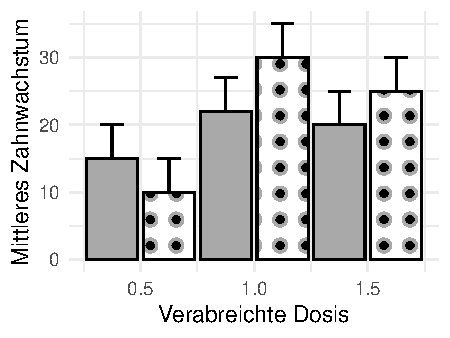
\includegraphics[width=\maxwidth]{img/mc-anova-02-a-1} 

}







\begin{enumerate}
\item [\textbf{A} \msquare] Keine Korrelation liegt vor $(p \geq 0.05)$.
\item [\textbf{B} \msquare] Eine mittlere bis starke Interaktion liegt vor $(p \leq 0.05)$
\item [\textbf{C} \msquare] Das Bestimmtheitsmaß $R^2$ ist groß.
\item [\textbf{D} \msquare] Die Koeffizienten sind negativ $(\beta_0 < 0; \beta_1 < 0)$.
\item [\textbf{E} \msquare] Keine Interaktion liegt vor $(p \leq 0.05)$.
\end{enumerate} 
\section*{Deskriptive Statistik \& Explorative Datenanalyse}

\section{Aufgabe \hfill (2 Punkte)}




Wie lautet der Mittelwert und Standardabweichung von $y$ mit 14, 16, 7, 10 und 9.



\begin{enumerate}
\item [\textbf{A} \msquare] Sie erhalten 11.2 +/- 1.85
\item [\textbf{B} \msquare] Es ergibt sich 10.2 +/- 6.85
\item [\textbf{C} \msquare] Es berechnet sich 12.2 +/- 13.7
\item [\textbf{D} \msquare] Es berechnet sich 11.2 +/- 13.7
\item [\textbf{E} \msquare] Sie erhalten 11.2 +/- 3.7
\end{enumerate} 

\section{Aufgabe \hfill (2 Punkte)}




Berechnen Sie den Median, das $1^{st}$ Quartile sowie das $3^{rd}$ Quartile von $y$ mit 11, 13, 23, 14, 11, 5, 18, 7, 3, 6 und 51.




\begin{enumerate}
\item [\textbf{A} \msquare] Es ergibt sich 11 +/- 6
\item [\textbf{B} \msquare] Sie erhalten 11 [4; 16]
\item [\textbf{C} \msquare] Es berechnet sich 12 [7; 17]
\item [\textbf{D} \msquare] Es ergibt sich 11 [6; 18]
\item [\textbf{E} \msquare] Es ergibt sich 15 +/- 6
\end{enumerate} 

\section{Aufgabe \hfill (2 Punkte)}



Die empfohlene Mindestanzahl an Beobachtungen für die Visualisierung mit einem Boxplot sind...



\begin{enumerate}
\item [\textbf{A} \msquare] Wir brauchen fünf oder mehr Beobachtungen.
\item [\textbf{B} \msquare] 1 Beobachtung.
\item [\textbf{C} \msquare] Die untere Grenze liegt bei einer Beobachtung.
\item [\textbf{D} \msquare] Die opimale Anzahl ist größer als hundert Beobachtungen, wobei es gerne sehr viel mehr sein können.
\item [\textbf{E} \msquare] 2-5 Beobachtungen.
\end{enumerate}

\section{Aufgabe \hfill (2 Punkte)}



Um die Standardabweichung zu berechnen müssen wir folgende Rechenoperationen durchführen.



\begin{enumerate}
\item [\textbf{A} \msquare] Wir berechnen erst den Mittelwert und dann die absoluten Abstände zu dem Mittelwert. Diese quadratischen Abstände summieren wir auf und teilen am Ende durch die Fallzahl.
\item [\textbf{B} \msquare] Den Mittelwert berechnen und die Abstände quadrieren. Die Summe mit der Fallzahl multiplizieren.
\item [\textbf{C} \msquare] Wir berechnen erst den Mittelwert und dann die quadratischen Abstände zu dem Mittelwert. Diese quadratischen Abstände summieren wir auf und teilen am Ende durch die Fallzahl. Als letzten Schritt ziehen wir die quadratische Wurzel.
\item [\textbf{D} \msquare] Den Mittelwert berechen, dann die absoluten Abstände zum Mittelwert aufsummieren
\item [\textbf{E} \msquare] Als erstes berechnen wir den Mittelwert. Dann bilden wir die Summe der quadratischen Abstände zu dem Mittelwert. Abschließend teilen wir durch die Fallzahl.
\end{enumerate} 

\section{Aufgabe \hfill (2 Punkte)}



Nachdem Sie eine ANOVA und die paarweisen t-Tests über das \Rlogo Paket \{emmeans\} durchgeführt haben, müssen Sie Ihre Daten nochmal zur Überprüfung visualisieren. Sie entscheiden sich für den Boxplot. Welche statistischen Maßzahlen stellt der Boxplot dar?

 



\begin{enumerate}
\item [\textbf{A} \msquare] Der Boxplot stellt den Median und die Quartile dar.
\item [\textbf{B} \msquare] Der Boxplot stellt den Median und die Streuung dar.
\item [\textbf{C} \msquare] Durch die Abbildung des Boxplot erhalten wir die Informationen über die Mittelwerte und die Varianz.
\item [\textbf{D} \msquare] Der Boxplot stellt die Mittelwerte und die Standardabweichung dar.
\item [\textbf{E} \msquare] Den Mittelwert und die Varianz.
\end{enumerate}

\section{Aufgabe \hfill (2 Punkte)}



In Ihrer Abschlussarbeit zuLauch finden Sie aufeinmal seltsame Daten. Jedenfalls kommt Ihnen das so vor. Daher berechnen Sie den Mittelwert und den Median. Der Mittelwert $\bar{y}$ und der Median $\tilde{y}$ unterscheiden sich. Welche Aussage ist richtig?



\begin{enumerate}
\item [\textbf{A} \msquare] Der Mittelwert und der Median sollten gleich sein, wenn Outlier in den Daten vorliegen. 
\item [\textbf{B} \msquare] Der Mittelwert und der Median sollten gleich sein, wenn keine Outlier in den Daten vorliegen. 
\item [\textbf{C} \msquare] Da sich der Mittelwert und der Median nicht unterscheiden, liegen vermutlich keine Outlier in den Daten vor. Wir verweden den Datensatz so wie er ist.
\item [\textbf{D} \msquare] Wenn sich der Mittelwert und der Median unterscheiden, liegen vermutlich keine Outlier in den Daten vor.
\item [\textbf{E} \msquare] Da sich der Mittelwert und der Median unterscheiden, ist der Datensatz nicht zu verwenden. Mittelwert und Median müssen gleich sein.
\end{enumerate}

\section{Aufgabe \hfill (2 Punkte)}



Ihre Betreuung der Abschlussarbeit fragt überraschend in der letzten Besprechung, ob Ihre Messwerte einer Normalverteilung genügen. Sonst könnten Sie ja gar nicht einen t-Test rechnen. Da Ihnen die Zeit wegrennt, entscheiden Sie sich für eine schnelle Visualisierung im Anhang. Welche Visualisierung nutzen Sie und welche Regel kommt zur Abschätzung einer Normalverteilung zur Anwendung?



\begin{enumerate}
\item [\textbf{A} \msquare] In einer explorativen Datanalyse nutzen wir den Violinplot. Dabei sollte der Bauch am Rand liegen. Dann können wir von einer Normalverteilung ausgehen.
\item [\textbf{B} \msquare] In einer explorativen Datanalyse nutzen wir den Boxplot. Dabei sollte der Median als dicke Linie in der Mitte der Box liegen. Dann können wir von einer Normalverteilung ausgehen.
\item [\textbf{C} \msquare] Nach dem Einlesen der Daten nutzen wir einen Boxplot um zu schauen, ob alle Boxen über alle Behandlungen in etwa gleich groß sind. Damit ist dann auch das IQR in allen Behandlungen in etwa gleich.
\item [\textbf{D} \msquare] Einen Barplot. Die Mittelwerte müssen alle auf einer Höhe liegen. Die Fehlerbalken haben hier keine Informationen.
\item [\textbf{E} \msquare] Einen Violinplot. Der Bauch der Violine muss hierbei einen höhren Wert annehmen als der Steg der Violine. Dann kann die Annahme einer Normalverteilung angenommen werden.
\end{enumerate}

\section{Aufgabe \hfill (2 Punkte)}




In der Statistik müssen wir häufig überprüfen, ob unser Outcome einer bestimmten Verteilung folgt. Meistens überprüfen wir, ob eine
Normalverteilung vorliegt. Folgende drei Abbildungen eigenen sich im Besonderen für die Überprüfung einer Verteilungsannahme an eine Variable.





\begin{enumerate}
\item [\textbf{A} \msquare] Histogramm, Scatterplot, Boxplot
\item [\textbf{B} \msquare] Violinplot, Scatterplot, Barplot
\item [\textbf{C} \msquare] Densityplot, Boxplot, Violinplot
\item [\textbf{D} \msquare] Barplot, Mosaicplot, Violinplot
\item [\textbf{E} \msquare] Histogramm, Densityplot, Dotplot
\end{enumerate} 

\section{Aufgabe \hfill (2 Punkte)}



Sie haben $n = 194$ Pflanzen geerntet und wollen sich nun die Verteilung der Pflanzen einmal in einem Histogramm anschauen. Welche Verteilung ist dargestellt?



{\centering 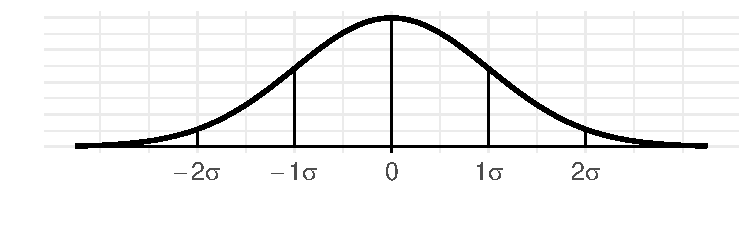
\includegraphics[width=\maxwidth]{img/mc-distribution-02-a-1} 

}







\begin{enumerate}
\item [\textbf{A} \msquare] Es handelt sich um eine Binomial-Verteilung.
\item [\textbf{B} \msquare] Wir haben eine Gammaverteilung vorliegen.
\item [\textbf{C} \msquare] Eine multivariate Normalverteilung.
\item [\textbf{D} \msquare] Es handelt sich um eine Normalverteilung.
\item [\textbf{E} \msquare] Dem Histogramm entnehmen wir eine Possion-Verteilung.
\end{enumerate} 
\section*{Lineare Regression \& Korrelation}

\section{Aufgabe \hfill (2 Punkte)}



Sie haben das Modell $Y \sim X$ vorliegen und wollen nun ein kausales Modell rechnen. Welche Aussage ist richtig?



\begin{enumerate}
\item [\textbf{A} \msquare] Wenn ein kausales Modell gerechnet werden soll, dann muss zum einen ein Traingsdatensatz sowie ein Testdatensatz definiert werden. Dabei ist der Trainingsdatensatz meist 1/10 und der Testdatensatz 1/3 der Fallzahl groß. Der Testdatensatz dient zur Validierung.
\item [\textbf{B} \msquare] Wenn ein kausales Modell gerechnet werden soll dann kann dies auf dem gesamten Datensatz geschehen. Das Ziel ist es einen Zusammenhang von $X$ auf $Y$ zu modellieren. Wie wirken sich die Einflussvariablen $X$ auf den gemessenen Endpunkt $Y$ aus?
\item [\textbf{C} \msquare] Es wird ein Trainingsdatensatz zum Modellieren des Trainingsmodells benötigt. Der Testdatensatz dient rein zur Visualisierung. Dies gilt vor allem für ein kausales Modell.
\item [\textbf{D} \msquare] Wenn ein kausales Modell gerechnet werden soll, dann muss zum einen ein Traingsdatensatz sowie ein Testdatensatz definiert werden. Dabei ist der Trainingsdatensatz meist 2/3 und der Testdatensatz 1/3 der Fallzahl groß. Der Testdatensatz dient zur Validierung.
\item [\textbf{E} \msquare] Ein kausales Modell schliesst grundsätzlich lineare Modell aus. Es muss ein Graph gefunden werden, der alle Punkte beinhaltet. Erst dann kann das $R^2$ berechnet werden.
\end{enumerate}

\section{Aufgabe \hfill (2 Punkte)}



Sie rechnen in eine linearen Regression und erhalten folgenden QQ Plot um die Annahme der normalverteilten Residuen zu überprüfen. Welche Aussage ist richtig?



{\centering 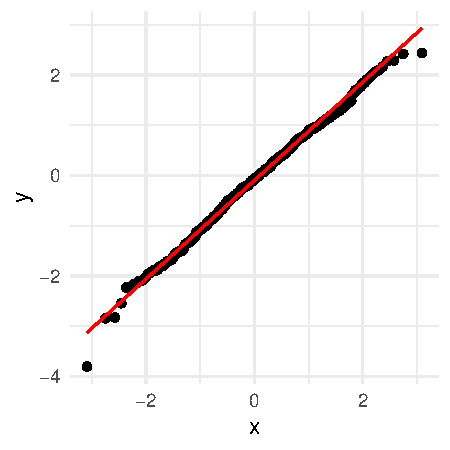
\includegraphics[width=\maxwidth]{img/mc-regression-05-a-1} 

}







\begin{enumerate}
\item [\textbf{A} \msquare] Wir betrachten die Gerade, die durch die einzelnen Punkte laufen sollte. Wenn die 95\% der Punkte von der Geraden getroffen werden, dann gehen wir von normalverteilten Residuen aus.
\item [\textbf{B} \msquare] Wir betrachten die Gerade und dabei insbesondere die beiden Enden der Gerade in dem IQR, also dem ersten und dritten Quartile. Hier sollten die Punkte auf der Geraden liegen, dann ist die Annahme an die Normalverteilung der Residuen erfüllt.
\item [\textbf{C} \msquare] Wir betrachten insbesondere die beiden Enden der Gerade. Der Rest ist mehr oder minder egal, dann ist die Annahme an die Normalverteilung der Residuen erfüllt.
\item [\textbf{D} \msquare] Wir betrachten die Gerade und dabei insbesondere die beiden Enden der Gerade. Hier sollten die Punkte auf der Geraden liegen, dann ist die Annahme an die Normalverteilung der Residuen erfüllt.
\item [\textbf{E} \msquare] Wir betrachten die Gerade. Wenn die Punkte einigermaßen gleichmäßig um die Gerade verteilt liegen, dann gehen wir von normalverteilten Residuen aus. Dies ist hier nicht der Fall. Wir haben keine normalverteilten Residuen vorliegen.
\end{enumerate}

\section{Aufgabe \hfill (2 Punkte)}



Nach einer Regressions sollten die Residuen (\texttt{.resid}) gleichmäßig um die Gerade verortet sein. Was bei einer simplen Regression noch relativ einfach visuell in einem Scatterplot zu überprüfen ist. Für komplexere Modell liefert der Residual Plot die notwendigen Informationen. Welche Aussage ist richtig?



{\centering 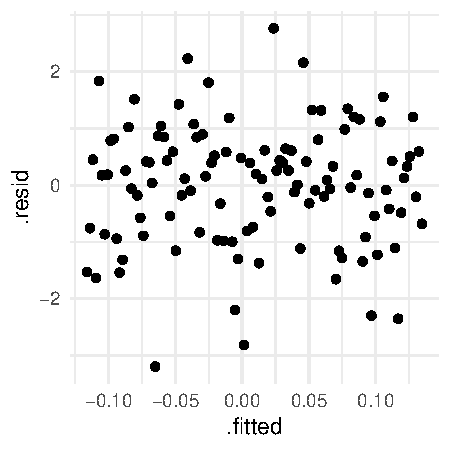
\includegraphics[width=\maxwidth]{img/mc-regression-06-a-1} 

}







\begin{enumerate}
\item [\textbf{A} \msquare] Die Punkte müssen gleichmäßig in dem negativen Bereich liegen. Dies ist hier klar nicht der Fall. Einzelne Ausreißer können beobachtet werden. Die Analyse ist gescheitert.
\item [\textbf{B} \msquare] Die Annahme der normalverteilten Residuen ist nicht erfüllt. Vereinzelte Punkte liegen oberhalb bzw. unterhalb der Geraden um die 0 Linie weiter entfernt. Ein klares Muster ist zu erkennen.
\item [\textbf{C} \msquare] Wenn wir die Nulllinie betrachten so liegen die Punkte nicht gleichmäßig über und unter der Nulllinie. Unser Modell erfüllt nicht die Annahme von normalverteilten Residuen mit einem Mittelwert von 0 und einer Streuung von $s^2$.
\item [\textbf{D} \msquare] Die Annahme der normalverteilten Residuen ist erfüllt. Die Punkte liegen zum überwiegenden Teil auf der Diagonalen. Damit ist das Modell erfolgreich geschätzt worden.
\item [\textbf{E} \msquare] Wenn die Punkte gleichmäßig in dem positiven wie auch negativen Bereich ohne ein klares Muster liegen, dann hat unsere Modellierung geklappt. Wir können mit dem Modell weitermachen.
\end{enumerate}

\section{Aufgabe \hfill (2 Punkte)}




In den Humanwissenschaften wird der Korrelationskoeffizienten $\rho$ sehr häufig verwendet. Daher ist es auch wichtig für andere Forschende den Korrelationskoeffizienten $\rho$ zu verstehen. Welche Aussazu zu dem Korrelationskoeffizienten $\rho$ ist richtig?




\begin{enumerate}
\item [\textbf{A} \msquare] Korrelationskoeffizienten $\rho$ liegt zwischen 0 und 1. Darüber hinaus ist der Korrelationskoeffizienten $\rho$ einheitslos und kann als Standardisierung verstanden werden.
\item [\textbf{B} \msquare] Der Korrelationskoeffizienten $\rho$ zeigt keinen Zusammenhang zwischen zwei Variablen $x$ und $y$ bei einem Wert von 0. Einen negativen Zusammenhang Richtung -1 und somit auch einen positiven Zusammenhang Richtung 1. Je größer die Zahl allgemein, desto stärker der Effekt.
\item [\textbf{C} \msquare] Der Korrelationskoeffizienten $\rho$ liegt zwischen -1 und 1. Darüber hinaus ist der Korrelationskoeffizienten $\rho$ als standardisierte Steigung zu verstehen, wenn eine Standardisierung durchgeführt wurde. Diese Adjustierung nach Fischer muss am Anschluß der Berechnung der Korrelation durchgeführt werden.
\item [\textbf{D} \msquare] Der Korrelationskoeffizienten $\rho$ liegt zwischen -1 und 1. Darüber hinaus ist der Korrelationskoeffizienten $\rho$ einheitslos und kann als standardisierte Steigung verstanden werden.
\item [\textbf{E} \msquare] Der Korrelationskoeffizienten $\rho$ wird wie das $\eta^2$ aus der ANOVA interpretiert. Der Korrelationskoeffizienten $\rho$ beschreibt den Anteil an erklärter Varianz durch die Regression. Dabei gibt er jedoch eine Richtung an und kann auch negativ werden.
\end{enumerate}

\section{Aufgabe \hfill (2 Punkte)}



In einer lineren Regression kann es vorkommen, dass der Effekt repräsentiert durch den $\beta$ Koeffizienten nicht so richtig von der Größenordnung zu dem p-Wert passen will. So liefert eine Untersuchung des Einflusses von der $PO_2$-Konzentration in [$\mu g$] im Wasser auf das Wachstum in [$kg$] an Spitzkohl folgende Effekte und p-Werte: $2e-04$ als p-Wert und einen $\beta_{PO_2}$ Koeffizienten von $1.1\times 10^{-5}$. Welche Aussage ist richtig?




\begin{enumerate}
\item [\textbf{A} \msquare] Die Einheit der $PO_2$-Konzentration ist zu klein gewählt. Dadurch sehen wir den sehr kleinen $p$-Wert. Der $p$-Wert und die Einheit von der $PO_2$-Konzentration hängen antiproportional zusammen.
\item [\textbf{B} \msquare] Die Einheit der $PO_2$-Konzentration ist zu klein gewählt. Die Erhöhung der $PO_2$-Konzentration um 1 Einheit führt nur zu einem sehr winzigen Anstieg von $\beta_{PO_2}$ im Gewicht der Wasserlinsen. Die Einheit [$\mu g$] muss besser gewählt werden.
\item [\textbf{C} \msquare] Die Fallzahl ist zu klein angesetzt. Je kleiner die Fallzahl ist, desto höher ist die Teststatsitik und damit auch der $p$-Wert kleiner. Wir brauchen also mehr Fallzahl um den geringen Effekt noch signifikant zu krigen.
\item [\textbf{D} \msquare] Wenn der Effekt $\beta_{PO_2}$ winzig ist, dann kann es an einer falsch gewählten Einheit liegen. Der Anstieg von einer Einheit in $X$ führt ja zu einer Änderung von $\beta_{PO_2}$ in $x$. Wir müssen daher die Einheit von $y$ entsprechend anpassen.
\item [\textbf{E} \msquare] Manchmal ist die Einheit der Einflussvariable $X$ zu groß gewählt, so dass der Ansteig von 1 Einheit in $X$ zu einer zu großen Änderung in $y$ führt. Daher kann der Effekt $\beta_{PO_2}$ sehr klein wirken, da der p-Wert wird auf einer einheitslosen Teststatistik bestimmt wird.
\end{enumerate}

\section{Aufgabe \hfill (2 Punkte)}



Nachdem Sie Ihr Experiment abgeschlossen haben, stehen Sie vor der Frage wie Sie Ihre Daten modellieren sollen. In der Beispielauswertung von Ihrem Betreuenden finden Sie die Funktion \texttt{lm()} in \Rlogo. Welche Aussage ist richtig?





\begin{enumerate}
\item [\textbf{A} \msquare] Ist die Einflussvariable $X$ numerisch so werden die Gruppenmittelwerte geschätzt und eine anschließende ANOVA sowie multipler Gruppenvergleich mit \{emmeans\} ist möglich.
\item [\textbf{B} \msquare] Neben der klassichen Verwendung der Funktion \texttt{lm()} in der linearen Regression kann auch ein Gruppenvergleich gerechnet werden. Dafür müssen aber alle Faktoren aus den Daten entfernt und numerishc umgewandelt werden. Dann kann das R Paket \{emmeans\} genutzt werden um die Korrelation zu berechnen. Eine Adjustierung ist dann nicht mehr notwendig.
\item [\textbf{C} \msquare] Die Funktion \texttt{lm()} in \Rlogo ist der erste Schritt für einen Gruppenvergleich. Danach kann eine ANOVA oder aber ein multipler Vergleich in \{emmeans\} gerechnet werden. In der Funktion  \texttt{lm()} werden die Gruppenmittelwerte bestimmt.
\item [\textbf{D} \msquare] Die Funktion \texttt{lm()} in \Rlogo ist der letzte Schritt für einen Gruppenvergleich. Vorher kann eine ANOVA oder aber ein multipler Vergleich in \{emmeans\} gerechnet werden. In der Funktion  \texttt{lm()} werden die Gruppenvarianzen bestimmt.
\item [\textbf{E} \msquare] Die Funktion \texttt{lm()} in \Rlogo wird klassischerweise für die nicht-lineare Regression genutzt. Ist die Einflussvariable $X$ numerisch so werden die Gruppenmittelwerte geschätzt.
\end{enumerate}

\section{Aufgabe \hfill (2 Punkte)}



In Ihrer Abschlussarbeit haben Sie neben den klassischen normalverteilten Endpunkte, wie Trockgewicht und Wuchshöhe noch den Infektionsstatus und Zähldaten erhoben. Um diese nicht normalverteilten Endpunkte auszuwerten nutzen Sie das \textit{generalisierte lineare Modell (GLM)}. Welche Aussage ist richtig?




\begin{enumerate}
\item [\textbf{A} \msquare] Dank dem \textit{generalisierten linearen Modell (GLM)} können auch andere Verteilungsfamilien als die Normalverteilung mit einer linearen Regression modelliert werden.
\item [\textbf{B} \msquare] Dank dem \textit{generalisierten linearen Modell (GLM)} können auch andere Verteilungsfamilien -- außer die Normalverteilung -- mit einer linearen Regression modelliert werden. Dafür werden alle Verteilungen in eine Normalverteilung überführt und anschließend standardisiert.
\item [\textbf{C} \msquare] Das GLM ist eine allgemeine Erweiterung der linearen Regression auf die Normalverteilung.
\item [\textbf{D} \msquare] Das \textit{generalisierte lineare Modell (GLM)} erlaubt auch weitere Verteilungsgruppen für das $X$ bzw. die Einflussvariablen in einer linearen Regression zu wählen.
\item [\textbf{E} \msquare] Das GLM erlaubt auch nicht normalverteilte Residuen in der Schätzung der Regressionsgrade.
\end{enumerate}
\section*{Vermischte Themen}  

\section{Aufgabe \hfill (2 Punkte)}

Die Randomisierung von Beobachtungen zu den Versuchseinheiten
ist bedeutend in der Versuchsplanung. Welche der folgenden Aussagen ist richtig?



\begin{enumerate}
\item [\textbf{A} \msquare] Strukturgleichheit ist durch Randomisierung gegeben. Leider hilft die Randomisierung noch nicht um von der Stichprobe auf die Grundgesamtheit zu schließen. Deshalb wurde das Falsifikationsprinzip entwickelt.
\item [\textbf{B} \msquare] Randomisierung sorgt für Strukturgleichheit und erlaubt erst von der Stichprobe auf die Grundgesamtheit zurückzuschliessen.
\item [\textbf{C} \msquare] Randomisierung erlaubt erst die Varianzen zu schätzen. Ohne eine Randomisierung ist die Berechnung von Mittelwerten und Varianzen nicht möglich. Dadurch lässt sich erst ein Experiment auswerten.
\item [\textbf{D} \msquare] Randomisierung ist die direkte Folge von Strukturgleichheit. Die Strukturgleichheit erlaubt es erst von der Stichprobe auf die Grundgesamtheit zurückzuschliessen.
\item [\textbf{E} \msquare] Randomisierung erlaubt erst die Mittelwerte zu schätzen. Ohne Randomisierung keine Mittelwerte. Ohne Mittelwerte keine Varianz und somit auch kein statistischer Test.
\end{enumerate}

\section{Aufgabe \hfill (2 Punkte)}



Wenn Sie einen Datensatz erstellen, dann ist es ratsam die Spalten und die Einträge in englischer Sprache zu verfassen, wenn Sie später die Daten in \Rlogo auswerten wollen. Welcher Aussage ist richtig?



\begin{enumerate}
\item [\textbf{A} \msquare] Programmiersprachen haben Probleme mit Umlauten und Sonderzeichen der deutschen Sprache. Daher ist die Nutzung in Deutsch in den AGBs von \Rlogo untersagt.
\item [\textbf{B} \msquare] Alle Funktionen und auch Anwendungen sind in \Rlogo in englischer Sprache. Die Nutzung von deutschen Wörtern ist nicht schick und das ist zu vermeiden.
\item [\textbf{C} \msquare] Im Allgemeinen haben Programmiersprachen Probleme mit Umlauten und Sonderzeichen, die in der deutschen Sprache vorkommen. Eine Nutzung der englischen Sprache umgeht dieses Problem auf einfache Art.
\item [\textbf{D} \msquare] Es gibt keinen Grund nicht auch deutsche Wörter zu verwenden. Es ist ein Stilmittel.
\item [\textbf{E} \msquare] Die Spracherkennung von \Rlogo ist nicht in der Lage Deutsch zu verstehen.
\end{enumerate}

\section{Aufgabe \hfill (2 Punkte)}



Bei der explorativen Datenanalyse (EDA) in \Rlogo gibt es eine richtige Abfolge von Prozessschritten, auch 	extit{Circle of life} genannt. Wie lautet die richtige Reihenfolge für die Erstellung einer EDA?



\begin{enumerate}
\item [\textbf{A} \msquare] Wir lesen die Daten ein und mutieren die Daten. Dabei ist wichtig, dass wir nicht das Paket \texttt{tidyverse} nutzen, da dieses Paket veraltet ist. über die Funktion \texttt{library(tidyverse)} entfernen wir das Paket von der Analyse.
\item [\textbf{B} \msquare] Wir transformieren die Spalten über \texttt{mutate()} in ein \texttt{tibble} und können dann über \text{ggplot()} uns die Abbildungen erstellen lassen. Dabei beachten wir das wir keine Faktoren in den Daten haben.
\item [\textbf{C} \msquare] Für eine explorativen Datenanalyse (EDA) in \Rlogo müssen wir als erstes die Daten über \texttt{read\_excel()} einlesen. Danach müssen wir schauen, dass wir die Spalten richtig über \texttt{mutate()} transformiert haben. Insbesondere müssen Variablen mit Kategorien in einen Faktor umgewandelt werden. Am Ende nutzen wir die Funktion \text{ggplot()} für die eigentlich EDA.
\item [\textbf{D} \msquare] Wir lesen die Daten über eine generische Funktion \texttt{read()} ein und müssen dann die Funktion \texttt{ggplot()} nur noch installieren. Dann haben wir die Abbildungen als \texttt{*.png} vorliegen.
\item [\textbf{E} \msquare] Die Funktionsreihenfolge ist wie folgt: \texttt{read\_excel()} ->  \texttt{mutate()} -> \text{ggplot()}. Dabei ist bei der Transformation der Daten darauf zu achten, dass keine Faktoren erstellt werden.
\end{enumerate}

\section{Aufgabe \hfill (2 Punkte)}



Sie haben das abstrakte Modell $Y \sim X$ mit $X$ als Faktor mit zwei Leveln vorliegen. Welche Aussage über $n_1 < n_2$ ist richtig?



\begin{enumerate}
\item [\textbf{A} \msquare] Es liegt Varianzhetrogenität vor.
\item [\textbf{B} \msquare] Es handelt sich um abhängige Beobachtungen.
\item [\textbf{C} \msquare] Es handelt sich um ein balanciertes Design.
\item [\textbf{D} \msquare] Es handelt sich um ein unbalanciertes Design.
\item [\textbf{E} \msquare] Es liegt Varianzhomogenität vor.
\end{enumerate}

\section{Aufgabe \hfill (2 Punkte)}



In einem Zuchtexperiment messen wir die Ferkel verschiedener Sauen. Die Ferkel einer Muttersau sind daher im statistischen Sinne...



\begin{enumerate}
\item [\textbf{A} \msquare] Untereinander abhängig, wenn die Mütter ebenfalls miteinander verwandt sind. Erst die Abhängigkeit 2. Grades wird in der Statistik modelliert.
\item [\textbf{B} \msquare] Untereinander unabhängig. Die Ferkel sind eigenständig und benötigen keine zusätzliche Behandlung.
\item [\textbf{C} \msquare] Die Ferkel stammen vom gleichen Muttertier und haben vermutlich eine ähnlichere Varianzstruktur als die Ferkel von anderen Sauen. Die Ferkel sind untereinander über die Mutter abhängig.
\item [\textbf{D} \msquare] Untereinander unabhängig. Sollten die Mütter verwandt sein, so ist die Varianzstruktur ähnlich und muss modelliert werden.
\item [\textbf{E} \msquare] Untereinander stark korreliert. Die Ferkel sind von einer Mutter und sommit miteinander korreliert. Dies wird in der Statistik jedoch meist nicht modelliert.
\end{enumerate}

\section{Aufgabe \hfill (2 Punkte)}



In einer Studie wollen Sie den Effektschätzer Odds ratio berechnen. Sie finden in Ihrem Experiment zur Behandlung von Klaueninfektionen bei Rinder in 4 Tieren Erkrankung der Klauen vor. 7 Tiere sind gesund. Welche Aussage ist richtig?



\begin{enumerate}
\item [\textbf{A} \msquare] Der Anteil der Kranken wird berechnet. Da es sich um ein Anteil handelt ergibt sich ein Odds ratio von 0.36.
\item [\textbf{B} \msquare] Es ergibt sich ein Odds ratio von 0.36, da es sich um eine Chancenverhältnis handelt.
\item [\textbf{C} \msquare] Da es sich um ein Chancenverhältnis handelt ergibt sich ein Odds ratio von 2.75.
\item [\textbf{D} \msquare] Der Anteil der Gesunden wird berechnet. Da es sich um ein Anteil handelt ergibt sich ein Odds ratio von 0.36.
\item [\textbf{E} \msquare] Da es sich um ein Chancenverhältnis handelt ergibt sich ein Odds ratio von 0.57.
\end{enumerate}

\section{Aufgabe \hfill (2 Punkte)}



In der Bio Data Science wird häufig mit sehr großen Datensätzen gerechnet. Historisch ergibt sich nun ein Problem bei der Auswertung der Daten und deren Bewertung hinsichtlich der Signifikanz. Welche Aussage ist richtig?





\begin{enumerate}
\item [\textbf{A} \msquare] Aktuell werden zu grosse Datensätze für die gänigige Statistik gemessen. Daher wendet man maschinelle Lernverfahren für kausale Modelle an. Hier ist die Relevanz gleich Signifikanz.
\item [\textbf{B} \msquare] Relevanz und Signifikanz haben nichts miteinander zu tun. Daher gibt es auch keinen Zusammenhang zwischen hoher Fahlzahl (n > 10000) und einem signifikanten Test. Ein Effekt ist immer relevant und somit signifikant.
\item [\textbf{C} \msquare] Aktuell werden immer größere Datensätze erhoben. Eine erhöhte Fallzahl führt automatisch auch zu mehr signifikanten Ergebnissen, selbst wenn die eigentlichen Effekte nicht relevant sind.
\item [\textbf{D} \msquare] Mehr Fallzahl in Datensätzen bedeutet mehr signifikante Ergebnisse, da in mehr Daten auch mehr Informationen beinhaltet sind. Deshalb lohnen sich riesige Datensätze, die durch die vielen signifikanten Ergebnisse auch eine Menge an relevanten Erkenntnissen liefern.
\item [\textbf{E} \msquare] Big Data ist ein Problem der parametrischen Statistik. Parameter lassen sich nur auf kleinen Datensätzen berechnen, da es sich sonst nicht mehr um eine Stichprobe im engen Sinne der Statistik handelt.
\end{enumerate}
\section*{Multiple Gruppenvergleiche}    

\section{Aufgabe \hfill (2 Punkte)}



Sie haben folgende unadjustierten p-Werte gegeben: 0.02, 0.01, 0.03 und 0.42. Sie adjustieren die p-Werte nach
Bonferroni. Welche Aussage ist richtig?



\begin{enumerate}
\item [\textbf{A} \msquare] Nach der Bonferroni-Adjustierung ergeben sich die adjustierten p-Werte von 0.005, 0.0025, 0.0075 und 0.105. Die adjustierten p-Werte werden zu einem $\alpha$-Niveau von 5\% verglichen.
\item [\textbf{B} \msquare] Nach der Bonferroni-Adjustierung ergeben sich die adjustierten p-Werte von 0.08, 0.04, 0.12 und 1.68. Die adjustierten p-Werte werden zu einem $\alpha$-Niveau von 5\% verglichen.
\item [\textbf{C} \msquare] Nach der Bonferroni-Adjustierung ergeben sich die adjustierten p-Werte von 0.005, 0.0025, 0.0075 und 0.105. Die adjustierten p-Werte werden zu einem $\alpha$-Niveau von 1.25\% verglichen.
\item [\textbf{D} \msquare] Nach der Bonferroni-Adjustierung ergeben sich die adjustierten p-Werte von 0.08, 0.04, 0.12 und 1. Die adjustierten p-Werte werden zu einem $\alpha$-Niveau von 5\% verglichen.
\item [\textbf{E} \msquare] Nach der Bonferroni-Adjustierung ergeben sich die adjustierten p-Werte von 0.08, 0.04, 0.12 und 1. Die adjustierten p-Werte werden zu einem $\alpha$-Niveau von 1.25\% verglichen.
\end{enumerate}

\section{Aufgabe \hfill (2 Punkte)}



Sie rechnen einen PostHoc-Test. Nun sollen Sie ein \textit{CLD} erstellen. Was bedeutet dieser Fachbegriff und welche folgende Beschreibung der Interpretation ist korrekt?



\begin{enumerate}
\item [\textbf{A} \msquare] Compact letter detection. Gleichheit in den Behandlungen wird durch den gleichen Buchstaben oder Symbol dargestellt.
\item [\textbf{B} \msquare] Compact letter display. Gleichheit in den Behandlungen wird durch den gleichen Buchstaben oder Symbol dargestellt. Teilweise ist die Interpretation des CLD herausfordernd, da wir ja nach dem Unterschied suchen.
\item [\textbf{C} \msquare] Compact line display. Gleichheit in den Behandlungen wird durch den gleichen Buchstaben oder Symbol dargestellt. Früher wurden keine Buchstaben sondern eine durchgezogene Linie verwendet. Bei mehr als drei Gruppen funktioniert die Linie aber graphisch nicht mehr.
\item [\textbf{D} \msquare] Compact letter display. Gleiche Buchstaben bedeuten, dass sich die Behandlungen unterscheiden. Daher ist das CLD sehr unintuitiv. Es wäre besser, wenn gleiche Buchstaben Gleichheit anzeigen würden. Dies ist aber leider in der statistischen Testtheorie nicht möglich.
\item [\textbf{E} \msquare] Compact letter display. Gleiche Buchstaben zeigen Gleichheit in den Behandlungen. Die Interpretation ist deshalb sehr intuitiv und einfach. Darüber hinaus ist damit das CLD auch auf einer Linie mit der Testtheorie, da wir ja auch dort die Gültigkeit der Nullhypothese nachweisen. Wir suchen ja Gleichheit.
\end{enumerate}

\section{Aufgabe \hfill (2 Punkte)}




Der multiple Vergleich als Posthoc-Test nach einer ANOVA ist in den Agrarwissenschaften heutzutage Standard. Welches R Paket wird häufig für den multiplen Vergleich genutzt? Welche Beschreibung der Eigenschaften ist korrekt?



\begin{enumerate}
\item [\textbf{A} \msquare] Das R Paket \{lm\}. Das Paket \{lm\} erstellt selbstständig Konfidenzintervalle und entsprechende p-Werte. Da wir in dem Paket nicht adjustieren müssen, ist es bei Anwendern sehr beliebt.
\item [\textbf{B} \msquare] Das R Paket \{emmeans\} erlaubt die Durchführung eines multiplen Gruppenvergleichs. Aus einem emmeans Objekt lässt sich leider kein CLD erstellen. Dennoch ist das Paket einfach zu bedienen und wird deshalb genutzt. Die Interpretation der statistischen Auswertung wird über einen Barplot abgebildet.
\item [\textbf{C} \msquare] Da Sie für Ihre Bachelorarbeit einen Barplot mit CLD brauchen nutzen Sie das R Paket \{emmeans\} welches Ihnen schnell die notwenidigen Informationen liefert um einen Barplot zu erstelen. Die Berechnung eines CLD ist hierbei auch einfach.
\item [\textbf{D} \msquare] Das R Paket \{ggplot\}. Wir erhalten hier sofort eine Visualisierung der Daten. Anhand der Visualisierung lässt sich eine explorative Datenanalyse durchführen, die gleichwertig zu einem Posthoc-Test ist.
\item [\textbf{E} \msquare] Das R Paket \{hmisc\} erlaubt die Durchführung eines multiplen Gruppenvergleichs aus verschiedenen Modellen heraus. Aus einem hmisc Objekt lässt sich recht einfach das CLD erstellen und so über Barplots eine schnelle Interpration der statistischen Auswertung durchführen.
\end{enumerate}

\section{Aufgabe \hfill (2 Punkte)}



Bei einem multiplen Vergleich oder Posthoc Test kann es zu einer Besonderheit beim statistischen Testen kommen. Wie nennt man diese Besonderheit beim statistischen Testen und wie kann man mit ihr umgehen?



\begin{enumerate}
\item [\textbf{A} \msquare] Beim multiplen Testen kann es zu einer $\beta$-Inflation kommen. Das globale Signifikanzniveau liegt nicht mehr bei $20\%$. Daher müssen die p-Werte entsprechend adjustiert werden. Hierfür gibt es verschiedene Verfahren, wobei das Verfahren zur Adjustierung der p-Werte nach Bonferroni das bekanneste Verfahren ist.
\item [\textbf{B} \msquare] Beim multiplen Testen kann es zu einer $\alpha$-Inflation kommen. Das globale Signifikanzniveau liegt nicht mehr bei $5\%$ sondern sehr viel höher. Daher müssen die p-Werte entsprechend adjustiert werden. Hierfür gibt es verschiedene Verfahren, wobei das Verfahren zur Adjustierung der p-Werte nach Bonferroni das bekanneste Verfahren ist.
\item [\textbf{C} \msquare] Das globale Signifikanzniveau liegt nicht mehr bei $5\%$ sondern sehr viel niedriger, bei ca. $1\%$. Es kommt zu einer $\alpha$-Hyperinflation. Dagegen kann mit der Adjustierung der p-Werte nach Bonferroni vorgegangen werden.
\item [\textbf{D} \msquare] Die Adjustierung der p-Werte nach Bonferroni erlaubt es gegen die $\beta$-Inflation vorzugehen, die häufig beim multiplen Testen auftritt. Das globale Powerniveau liegt nicht mehr bei $80\%$ sondern sehr viel niedriger.
\item [\textbf{E} \msquare] Beim multiplen Testen kann es zu einer $\alpha$-Inflation kommen. Das globale Signifikanzniveau liegt nicht mehr bei $5\%$ sondern weit darunter. Daher müssen die p-Werte entsprechend adjustiert werden. Hierfür gibt es verschiedene Verfahren, wobei das Verfahren zur Adjustierung der p-Werte nach Welch das bekanneste Verfahren ist.
\end{enumerate}

\section{Aufgabe \hfill (2 Punkte)}




In Ihrer Bachelorarbeit werten Sie einen einfaktoriellen Versuch aus. Dafür rechnen Sie in \Rlogo zunächst eine ANOVA und schließen dann dann einen multiplen vergleich mit t-Tests an. Welche Aussage über die Effekte in Ihrem versuch ist richtig?



\begin{enumerate}
\item [\textbf{A} \msquare] Wenn ein multipler Test gerechnet wird, dann muss der Effekt $\Delta$ adjustiert werden im Gegensatz zu den p-Werten.
\item [\textbf{B} \msquare] Wenn ein multipler Test gerechnet wird, dann muss der Effekt $\Delta$ nach Bonferroni adjustiert werden. Dafür wird der Effekt mit der Anzahl an Vergleichen $k$ multipliziert. Dies geschiet analog zu den p-Werten.
\item [\textbf{C} \msquare] Beim multiplen Testen kann es zu einer $\Delta$-Deflation kommen. Das globale Relevanzniveau liegt nicht mehr bei $5\%$ sondern weit darunter. Daher müssen die $\Delta$-Werte entsprechend adjustiert werden. Hierfür gibt es verschiedene Verfahren, wobei das Verfahren zur Adjustierung der $\Delta$-Werte nach Bonferroni das bekanneste Verfahren ist. Die $\Delta$-Werte werden durch die Anzahl an Vergleichen geteilt.
\item [\textbf{D} \msquare] Beim multiplen Testen muss der Effekt, wie der Mittelwertsunterschied $\Delta$ aus einem t-Test, nicht adjusiert werden.
\item [\textbf{E} \msquare] Wenn ein multipler Test gerechnet wird, dann muss der Effekt $\Delta$ nicht adjustiert werden. Bei einem Effekt im multiplen Testen handelt es sich um eine Wahrscheinlichkeit für das Auftreten der Nullhypothese.
\end{enumerate}
\section*{Statistische Testtheorie}  

\section{Aufgabe \hfill (2 Punkte)}




Welche Aussage zum mathematische Ausdruck $Pr(D|H_0)$ ist richtig?



\begin{enumerate}
\item [\textbf{A} \msquare] Die Wahrscheinlichkeit der Daten unter der Nullhypothese in der Grundgesamtheit.
\item [\textbf{B} \msquare] Die Wahrscheinlichkeit für die Nullhypothese, wenn die Daten wahr sind.
\item [\textbf{C} \msquare] $Pr(D|H_0)$ stellt die Wahrscheinlichkeit die Teststatistik $T$ zu beobachten dar, wenn die Nullhypothese falsch ist.
\item [\textbf{D} \msquare] $Pr(D|H_0)$ ist die Wahrscheinlichkeit die Daten $D$ zu beobachten, wenn die Nullhypothese wahr ist.
\item [\textbf{E} \msquare] Die Inverse der Wahrscheinlichkeit unter der die Nullhypothese nicht mehr die Alternativehypothese überdeckt.
\end{enumerate}

\section{Aufgabe \hfill (2 Punkte)}



Die Testtheorie hat einen philosophischen Unterbau. Eins der Prinzipien ist das Falsifikationsprinzip. Das Falsifikationsprinzip besagt,



\begin{enumerate}
\item [\textbf{A} \msquare] ... dass Modelle meist falsch sind und selten richtig.
\item [\textbf{B} \msquare] ... dass ein schlechtes Modell durch das Falsifikationsprinzip durch ein weniger schlechtes Modell ersetzt wird.
\item [\textbf{C} \msquare] ... dass Annahmen an statistische Modelle meist falsch sind.
\item [\textbf{D} \msquare] ... dass ein minderwertes Modell durch ein minderwertiges Modell ersetzt wird. Es gilt das Verifikationsprinzip nach Karl Popper.
\item [\textbf{E} \msquare] ... dass in der Wissenschaft immer etwas falsch sein muss. Sonst gebe es keinen Fortschritt.
\end{enumerate}

\section{Aufgabe \hfill (2 Punkte)}



Das Signifikanzniveau $\alpha$ wird auch Fehler 1. Art genannt und liegt bei 5\%. Warum wurde der Grenzwert von 5\% als Signifikanzschwelle gewählt?



\begin{enumerate}
\item [\textbf{A} \msquare] Der Begründer der modernen Statistik, R. Fischer, hat die Grenze simuliert und berechnet. Dadurch ergibt sich dieser optimale Cut-Off.
\item [\textbf{B} \msquare] Da Wissenschaftler eine Schwelle für die statistische Testentscheidung benötigen wurde $\alpha$ historisch gewählt. Damit ist $\alpha = 5\%$ eine Kulturkonstante.
\item [\textbf{C} \msquare] Im Rahmen eines langen Disputs zwischen Neyman und Fischer wurde $\alpha = 5\%$ festgelegt. Leider werden die Randbedingungen und Voraussetzungen an statistsiche Modelle heute immer wieder ignoriert.
\item [\textbf{D} \msquare] Auf einer Statistikkonferenz in Genf im Jahre 1942 wurde dieser Cut-Off nach langen Diskussionen festgelegt. Bis heute ist der Cut Off aber umstritten, da wegen dem 2. Weltkrieg viele Wissenschaftler nicht teilnehmen konnten.
\item [\textbf{E} \msquare] Der Wert ergab sich aus einer Auswertung von 1042 wissenschaftlichen Veröffentlichungen zwischen 1914 und 1948. Der Wert $5\%$ wurde in $28\%$ der Veröffentlichungen genutzt. Daher legte man sich auf diese Zahl fest.
\end{enumerate}

\section{Aufgabe \hfill (2 Punkte)}

Betrachten wir die Teststatistik aus einem abstrakteren Blickwinkel. Beim
statistischen Testen wird das \textit{"`signal"'} mit dem
\textit{"`noise"'} aus den Daten $D$ zu einer Teststatistik $T_D$ verrechnet. Welche der Formel
berechnet korrekt die Teststatistik $T_D$?



\begin{enumerate}
\item [\textbf{A} \msquare] Es gilt $T_D = \cfrac{signal}{noise^2}$
\item [\textbf{B} \msquare] Es gilt $T_D = signal \cdot noise$
\item [\textbf{C} \msquare] Es gilt $T_D = \cfrac{noise}{signal}$
\item [\textbf{D} \msquare] Es gilt $T_D = \cfrac{signal}{noise}$
\item [\textbf{E} \msquare] Es gilt $T_D = (signal \cdot noise)^2$
\end{enumerate}

%% ------------------------------------------------------------

\section{Aufgabe \hfill (2 Punkte)}



In der Theorie zur statistischen Testentscheidung kann folgende Aussage
in welche richtige Analogie gesetzt werden?

\begin{center}
\textit{$H_0$ ablehnen obwohl die $H_0$ gilt}
\end{center}



\begin{enumerate}
\item [\textbf{A} \msquare] In die Analogie eines Feuerwehrautos: \textit{Car without noise}.
\item [\textbf{B} \msquare] In die Analogie eines Rauchmelders: \textit{Alarm without fire police}, dem $\alpha$-Fehler.
\item [\textbf{C} \msquare] \textit{Alarm without fire}, dem $\alpha$-Fehler in der Analogie eines Rauchmelders.
\item [\textbf{D} \msquare] In die Analogie eines Rauchmelders: \textit{Alarm with fire}.
\item [\textbf{E} \msquare] Dem $\beta$-Fehler mit der Analogie eines Rauchmelders: \textit{Fire without alarm}.
\end{enumerate}

\section{Aufgabe \hfill (2 Punkte)}



Sie sollen in Ihrer Abschlussarbeit die Relevanz und die Signifikanz in einer statistischen Maßzahl vereinen. Welche Aussage ist richtig?



\begin{enumerate}
\item [\textbf{A} \msquare] Das $\Delta$. Durch die Effektstärke haben wir einen Wert für die Relevanz, die vom Anwender bewertet werden muss. Da $\Delta$ antiproportional zum p-Wert ist, bedeutet auch ein hohes $\Delta$ ein sehr kleinen p-Wert.
\item [\textbf{B} \msquare] Das OR. Als Chancenverhältnis gibt es das Verhältnis von Relevanz und Signifikanz wieder.
\item [\textbf{C} \msquare] Einem Konfidenzintervall. Das Konfidenzinterval bringt durch eine Visualisierung und drei Intervallgrenzen die Möglichkeit mit, eine Relevanzschwelle neben der Signifikanzschwelle und der $\alpha$-Schwelle zu definieren.
\item [\textbf{D} \msquare] Über das Konfidenzintervall. Das Konfidenzinterval beitet eine Entscheidung über die Signifikanz und zusätzlich kann über die Visualizierung des Konfidenzintervals eine Relevanzschwelle definiert werden.
\item [\textbf{E} \msquare] Über das Konfidenzintervall. Das Konfidenzinterval inkludiert eine Entscheidung über die Relevanz und zusätzlich kann über die Visualizierung des Konfidenzintervals eine Signifikanzschwelle vom Forschenden definiert werden.
\end{enumerate}

\section{Aufgabe \hfill (2 Punkte)}



Welche Aussage über den $p$-Wert und dem Signifikanzniveau $\alpha$ gleich 5\% ist richtig?



\begin{enumerate}
\item [\textbf{A} \msquare] Wir machen ein Aussage über die Flächen und zwischen den Kurve der Teststatistiken der Hypothesen $H_0$ und $H_A$, wenn die $H_0$ gilt. Dabei werden Wahrscheinlichkeiten vergleichen, die durch die Flächen unter der Kurve repräsentiert werden.
\item [\textbf{B} \msquare] Wir vergleichen mit dem $p$-Wert und dem Signifikanzniveau $\alpha$ absolute Werte auf einem Zahlenstrahl und damit den Unterschied der Teststatistiken, wenn die $H_0$ gilt.
\item [\textbf{C} \msquare] Wir schauen, ob der $p$-Wert kleiner ist als das Signifikanzniveau $\alpha$ und vergleichen somit Wahrscheinlichkeiten. Die Wahrscheinlichkeiten werden als Flächen unter der Kurve der Teststaistik dargestellt, wenn die $H_0$ gilt.
\item [\textbf{D} \msquare] Wir machen eine Aussage über die indivduelle Wahrscheinlichkeit des Eintretens der Nullhypothese $H_0$. Der $p$-Wert wird mit dem Signifikanzniveau verglichen und bewertet.
\item [\textbf{E} \msquare] Wir schauen, ob der $p$-Wert größer ist als das Signifikanzniveau $\alpha$ und vergleichen somit Wahrscheinlichkeiten. Die Wahrscheinlichkeiten werden als Flächen unter der Kurve der Teststaistik dargestellt, wenn die $H_A$ gilt.
\end{enumerate}

\section{Aufgabe \hfill (2 Punkte)}



Um die Testtheorie besser zu verstehen, mag es manchmal sinnvoll sein ein Beispiel aus dem Alltag zu wählen. Die Ergebnisse der Analyse durch einen statistischen Test können auch in grobe Analogie zur Wettervorhersage gebracht werden. Welche Aussage trifft am ehesten zu?



\begin{enumerate}
\item [\textbf{A} \msquare] In der Analogie der Regenwahrscheinlichkeit in einem bestimmten Gebiet: ein statistischer Test gibt die Wahrscheinlichkeit für ein Ereignis in einem Experiment mit den Daten $D$ wieder und lässt sich kaum verallgemeinern.
\item [\textbf{B} \msquare] In der Analogie der Maximaltemperatur: Was ist der maximale Unterschied zwischen zwei Gruppen. Wir erhalten hier eine Aussage über die Spannweite und den maximalen Effekt.
\item [\textbf{C} \msquare] In der Analogie der Wahrscheinlichkeit für Regen: ein statistischer Test erlaubt die Wahrscheinlichkeit für ein Ereignis abzuschätzen. Die Stärke des Effektes können wir nicht bestimmen.
\item [\textbf{D} \msquare] In der Analogie des Niederschlags oder Regenmenge: ein statistischer Test gibt die Stärke eines Effektes wieder. Zum Beispiel, wie hoch ist der Mittelwertsunterschied.
\item [\textbf{E} \msquare] In der Analogie der Sonnenscheindauer: Wie lange kann mit einem entsprechenden Effekt gerechnet werden? Die Wahrscheinlichkeit für den Effekt gibt der statistische Test wieder.
\end{enumerate}

\section{Aufgabe \hfill (2 Punkte)}



In Ihrer Forschungsarbeit wollen Sie eine Aussage über die untersuchte Population treffen. Dazu nutzen Sie eine ANOVA als statistischen Test. Erhalten Sie eine valide Aussage aus einem statistischen Test?



\begin{enumerate}
\item [\textbf{A} \msquare] Nein, wir erhalten eine Aussage. Müssen aber das Individuum im Kontext der Population adjustieren.
\item [\textbf{B} \msquare] Nein, es ist nicht möglich die untersuchte Population mit einem t-Test auszuwerten. Wir erhalten dann leider keine Aussage zur Population.
\item [\textbf{C} \msquare] Ja, es ist möglich die untersuchte Population mit einem t-Test auszuwerten. Wir erhalten dann eine Aussage zur Population.
\item [\textbf{D} \msquare] Ja, wir erhalten nur eine Aussage zu zwei Individuen. Ein statistischer Test liefert Informationen zu einem Individuum im Vergleich zu einem anderen Individuum.
\item [\textbf{E} \msquare] Nein, wir können die untersuchte Population nicht mit einem t-Test auswerten. Wir erhalten keine Aussage zur Population. Wir können aber den Effekt als Quelle der Relevanz nutzen.
\end{enumerate}

\section{Aufgabe \hfill (2 Punkte)}



In der statistischen Testtheorie gibt es den Begriff \textit{Power}. Was sagt der statistische Begriff \textit{Power} aus?



\begin{enumerate}
\item [\textbf{A} \msquare] Es gilt $\alpha + \beta = 1$ und somit liegt $\beta$ meist bei 95\%.
\item [\textbf{B} \msquare] Die Power ist nicht in der aktuellen Testthorie mehr vertreten. Wir rechnen nur noch mit dem Fehler 1. Art.
\item [\textbf{C} \msquare] Alle statistischen Tests sind so konstruiert, dass die $H_A$ mit 80\% \textit{bewiesen wird}. Die Power ist $1-\beta$ mit $\beta$ gleich 20\% gesetzt.
\item [\textbf{D} \msquare] Alle statistischen Tests sind so konstruiert, dass die $H_A$ mit 20\% \textit{bewiesen wird}. Die Power ist $1-\beta$ mit $\beta$ gleich 80\% gesetzt.
\item [\textbf{E} \msquare] Die Power wird berechnet und ist keine Eigenschaft des Tests. Die Power wird auf $80\%$ gesetzt und beschreibt mit welcher Wahrscheinlichkeit $H_0$ \textit{bewiesen wird}
\end{enumerate}

\section{Aufgabe \hfill (2 Punkte)}



Welche Aussage über den Effekt eines statistischen Tests ist richtig?



\begin{enumerate}
\item [\textbf{A} \msquare] Der Effekt eines statistischen Tests beschreibt die biologisch interpretierbare Ausgabe eines Tests. Moderen Algorithmen liefern keine Effekte mehr sondern nur noch bedingte Wahrscheinlichkeiten. Der Effekt spielt in der modernen Statistik keine Rollen mehr.
\item [\textbf{B} \msquare] Der Effekt eines statistischen Tests beschreibt die biologisch interpretierbare Ausgabe eines Tests. Zum Beispiel den mittleren Unterschied zwischen zwei Gruppen aus einem t-Test. Damit ist der Effekt direkt mit dem Begriff der Relevanz verbunden. Die Entscheidung über die Relevanz trifft der Forschende unabhängig von der Signifikanz eines statistischen Tests.
\item [\textbf{C} \msquare] Der Effekt eines statistischen Tests beschreibt die biologisch interpretierbare Ausgabe eines Tests. Damit ist der Effekt direkt mit dem Begriff der Signifikanz verbunden. Die Entscheidung über die Signifikanz trifft der Forschende unabhängig von der Relevanz eines statistsichen Tests.
\item [\textbf{D} \msquare] Durch den Effekt erfahren wir die statistische interpretierbare Ausgabe eines statistischen Tests. Zum Beispiel das $\eta^2$ aus einer ANOVA. Damit können wir die Signifikanz direkt mit dem Effekt verbinden. Am Ende muss der Forschende aber entscheiden, ob der Effekt entsprechend seinen Erwartungen als bedeutet zu bewerten ist.
\item [\textbf{E} \msquare] Der Effekt eines statistischen Tests beschreibt die mathematisch interpretierbare Ausgabe eines Tests. Damit ist der Effekt direkt mit dem Begriff der Signifikanz verbunden. Die Entscheidung über die Signifikanz trifft der Forschende unabhängig von der Relevanz eines statistsichen Tests.
\end{enumerate}

\section{Aufgabe \hfill (2 Punkte)}



Welche Aussage über die Entscheidung anhand des p-Wertes gegen die
Nullhypothese ist richtig?



\begin{enumerate}
\item [\textbf{A} \msquare] Ist $Pr(D|H_0)$ kleiner als das Signifikanzniveau $\alpha$ gleich $5\%$ dann wird die Nullhypothese $H_0$ abgelehnt.
\item [\textbf{B} \msquare] Ist $T_{D}$ h{"o}her als der kritische Wert $T_{\alpha = 5\%}$ dann wird die Nullhypothese $H_0$ abgelehnt.
\item [\textbf{C} \msquare] Ist in dem 95\%-Konfidenzintervall nicht die Null enthalten dann wird die Nullhypothese $H_0$ abgelehnt.
\item [\textbf{D} \msquare] Anhand des p-Wertes lässt sich wie folgt eine Entscheidung treffen. Liegt der Wert in dem Signifikanzniveauintervall $\alpha$ dann kann die Nullhypothese abgelehnt werden.
\item [\textbf{E} \msquare] Anhand des p-Wertes lässt sich wie folgt eine Entscheidung treffen. Liegt der Wert über oder gleich dem Signifikanzniveau $\alpha$ dann kann die Nullhypothese abgelehnt werden.
\end{enumerate}

\section{Aufgabe \hfill (2 Punkte)}



Wenn Sie im Allgemeinen einen statistischen Test rechnen, dann kommen Sie um eine statistische Hypothese $H$ nicht herum. Welche Aussage über statistische Hypothesen ist richtig?



\begin{enumerate}
\item [\textbf{A} \msquare] Mit der Nullhypothese $H_0$ und der Alternativehypothese $H_A$ oder $H_1$ gibt es zwei Hypothesen.
\item [\textbf{B} \msquare] Es gibt - bedingt durch das das Falsifikationsprinzip - ein Set von $k$ Nullhypothesen, die iterative gegen $k-1$ Alternativhypothesen getestet werden.
\item [\textbf{C} \msquare] Die Hypothesen $H_0$ und $H_A$ sind rein prosarischer Natur und bilden keinen mathematischen Hintergrund ab. In der Statistik wird die wissenschaftliche Fragestellung getestet. Daher stehen auch die verständlichen Hypothesen im Mittelpunkt der biologischen Interpretation.
\item [\textbf{D} \msquare] Mit der Nullhypothese $H_A$ und der Alternativehypothese $H_0$ gibt es zwei Hypothesen, die aber selten genutzt werden.
\item [\textbf{E} \msquare] Es gibt ein Hypothesenset bestehend aus $k$ Hypothesen. Meistens wird die Nullhypothese $H_0$ und die Alternativhypothese $H_A$ verwendet. Wegen des Falsifikationsprinzips ist es wichtig, die bekannte falsche und unbekannte richtige Hypothese mit in das Set zu nehmen.
\end{enumerate}
\section*{Statistische Tests für Gruppenvergleiche} 

\section{Aufgabe \hfill (2 Punkte)}



Welche Aussage über den t-Test im Allgmeinen ist richtig? Berücksichtigen Sie den Welch t-Test wie auch den Student t-Test!



\begin{enumerate}
\item [\textbf{A} \msquare] Der t-Test vergleicht zwei Gruppen indem die Mittelwerte miteinander verglichen werden.
\item [\textbf{B} \msquare] Der t-Test testet generell zu einem erhöhten $\alpha$-Niveau von 20\%.
\item [\textbf{C} \msquare] Der t-Test vergleicht die Mittelwerte von zwei Gruppen unter der strikten Annahme von Varianzhomogenität. Sollte keine Varianzhomogenität vorliegen, so gibt es keine Möglichkeit den t-Test in einer Variante anzuwenden.
\item [\textbf{D} \msquare] Der t-Test vergleicht zwei oder mehr Gruppen indem die Mittelwerte miteinander verglichen werden.
\item [\textbf{E} \msquare] Der t-Test vergleicht die Varianzen von mindestens zwei oder mehr Gruppen
\end{enumerate}

\section{Aufgabe \hfill (2 Punkte)}



Ein Versuch wurde in 13 Parzellen pro Gruppe durchgeführt. Die folgende Abbildung enthält die Daten aus diesem Versuch zur Bewertung der Wirkung des Mikronährstoff Eisen auf den Ertrag in t/ha von Weizen im Vergleich zu einer Kontrolle.  Welche Aussage ist richtig, wenn Sie einen t-Test rechnen?



{\centering 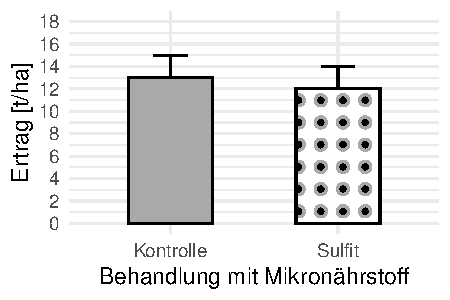
\includegraphics[width=\maxwidth]{img/mc-testing-ttest-02-1} 

}







\begin{enumerate}
\item [\textbf{A} \msquare] Es liegt ein signifikanter Unterschied vor. Der Effekt liegt bei -0.7.
\item [\textbf{B} \msquare] Nach Betrachtung des Barplots liegt kein signifikanter Unterschied vor. Der Effekt kann nicht bei einem t-Test aus Barplots bestimmt werden.
\item [\textbf{C} \msquare] Der Test deutet auf ein signifikanten Unterschied hin. Der Effekt liegt vermutlich bei -7.
\item [\textbf{D} \msquare] Die Barplots deuten auf keinen signifikanten Unterschied. Der Effekt liegt vermutlich bei -7 unter einer groben Abschätzung.
\item [\textbf{E} \msquare] Der Effekt und die Signifikanz lassen sich nicht aus Barplots abschätzen. Höchtens der Effekt als relativer Unterschied zwischen der Höhe der Barplots. Standard ist der mediane Unterschied aus Boxplots.
\end{enumerate}

\section{Aufgabe \hfill (2 Punkte)}




Welche Aussage über den gepaarten t-Test für verbundene Stichproben ist richtig?



\begin{enumerate}
\item [\textbf{A} \msquare] Abhängige Beobachtungen müssen gesondert in einem gepaarten t-Test modelliert werden. Wenn wiederholt an dem gleichen Tier oder Pflanze gemessen wird, dann bilden wir den Quotienten zwischen den beiden Zeitpunkten. Auf den Quotienten rechnen wir den gepaarten t-Test.
\item [\textbf{B} \msquare] Beim gepaarten t-Test kombinieren wir die Vorteile des Student t-Test für Varianzhomogenität mit den Vorteilen des Welch t-Test für Varianzheterogenität. Wir bilden dafür die Differenz der Einzelbeobachtungen.
\item [\textbf{C} \msquare] Abhängige Beobachtungen müssen gesondert in einem gepaarten t-Test modelliert werden. Wenn wiederholt an dem gleichen Tier oder Pflanze gemessen wird, dann bilden wir die Differenz zwischen den beiden Zeitpunkten. Auf den Differenzen rechnen wir den gepaarten t-Test.
\item [\textbf{D} \msquare] Der gepaarte t-Test wird gerechnet, wenn die Beobachtungen abhängig voneinander sind. Wir messen jede Beobachtung nur einmal und berechnen dann die Differenz zu dem Mittel der anderen Beobachtungen.
\item [\textbf{E} \msquare] Wenn die Beobachtungen unabhängig voneinander sind, rechnen wir einen gepaarten t-Test. Messen wir wiederholt an dem gleichen Tier oder Pflanze dann bilden wir das Produkt zwischen den zwei Messpunkten.
\end{enumerate}

\section{Aufgabe \hfill (2 Punkte)}



In Ihrer Abschlussarbeit passen die Ergebnisse einer ANOVA und eines multiplen Vergleiches nicht zusammen. Nach einem Experiment mit vier Maissorten ergibt eine ANOVA ($p = 0.049$). Sie führen anschließend die paarweisen t-Tests für alle Vergleiche durch. Nach der Adjustierung für multiples Testen ist kein p-Wert unter der $\alpha$-Schwelle. Sie schauen sich auch die rohen, unadjustierten p-Werte an und finden hier als niedrigsten p-Wert $p_{3-2} = 0.052$. Welche Aussage ist richtig?




\begin{enumerate}
\item [\textbf{A} \msquare] Die adjustierten p-Werte deuten in die richtige Richtung. Zusammen mit den nicht signifikanten rohen p-Werten ist von einem Fehler in der ANOVA auszugehen.
\item [\textbf{B} \msquare] Das ist kein Wunder. Die ANOVA testet auf der gesamten Fallzahl und die paarweisen t-Tests verlieren immer eine oder mehr Gruppen als Fallzahl. Mit steigender Fallzahl sind mehr signifikante Unterschiede zu erwarten. Die p-Werte unterscheiden sich numerisch auch kaum.
\item [\textbf{C} \msquare] Der Fehler liegt in den t-Tests. Wenn eine ANOVA signifikant ist, dann muss zwangsweise auch ein t-Test signifikant sein.
\item [\textbf{D} \msquare] Es gibt einen Fehler in der Varianzstruktur. Daher kann die ANOVA nicht richtig sein und paarweise t-Tests liefern das richtige Ergebnis.
\item [\textbf{E} \msquare] Hier kommt der Effekt der stiegenden Fallzahl auf die Anzahl an signifikante Ergebnisse zu tragen. Da die ANOVA auf weniger Fallzahl testet als die paarweisen t-Tests, kann die ANOVA schwerer einen signifikanten Unterscheid nachweisen.
\end{enumerate}
    
% -----------------------------------------------------------------------
\clearpage
% -----------------------------------------------------------------------
\part{Deskriptive Statistik \& Explorative Datenanalyse}
% -----------------------------------------------------------------------

\section{Aufgabe \hfill (8 Punkte)}

\textit{Geben Sie grundsätzlich Formeln und Rechenweg zur Lösung der Teilaufgaben mit an!} \\[1Ex]
 

 
%% --------------------------------------------------------------------
\begin{minipage}[t]{0.5\textwidth}

\includegraphics[width = 1.3cm]{/Users/kruppajo/work/GitHub/exam/avatare/Jonas.png}
\end{minipage}
\begin{minipage}[t]{0.5\textwidth}
\hfill
\href{https://youtu.be/t0WYa_LVc5o}{
\includegraphics[width = 2cm]{img/youtube}}
\end{minipage}
\vspace{-3ex}
%% --------------------------------------------------------------------



\paragraph{Zerforschen des Barplots}

Jonas steht vor einem ersten Problem, denn wenn es nach seiner Betreuerin geht, soll er in einem einer Klimakammer Erdbeeren auswertet. Soweit eigentlich alles passend. Besser wäre was anderes gewesen. Am Ende dann doch besser Stricken. Wunderbar. Eine echte Ablenkung für Jonas. Das heißt erstmal überlegen für Jonas. Aus den Boxen wummert Iron Maiden und sein Mund ist verklebt von Snickers. 'Herrlich', denkt Jonas. Die Behandlung werden verschiedene Genotypen ($AA$, $AB$ und $BB$) sein. In seiner Exceldatei wird er den Endpunkt ($Y$) \textit{Ertrag} als \textit{yield} aufnehmen. Vorab soll Jonas aber eimal die folgenden Barplots seiner Betreuerin nachbauen, damit er den \Rlogo Code schonmal für später vorliegen hat. Damit geht das Problem schon los. Wenn die Erschöpfung nicht wäre, ja dann wäre wohl vieles möglich für Jonas! Aber so..



{\centering 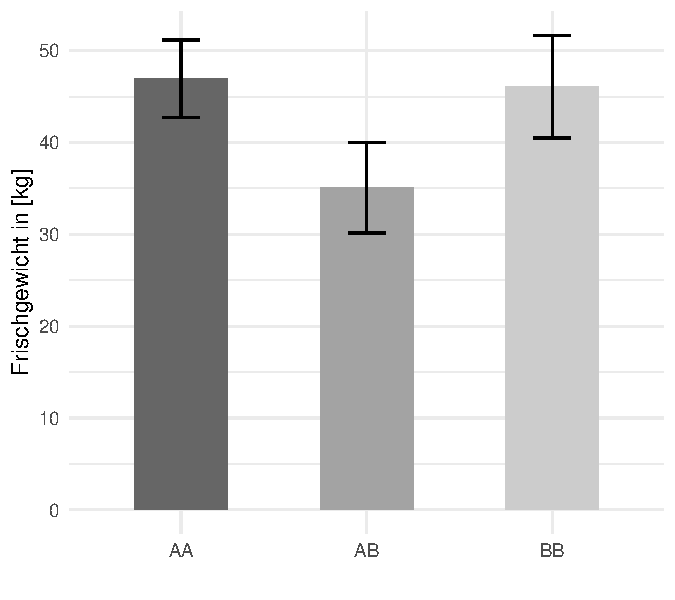
\includegraphics[width=\maxwidth]{img/barplot-02-1} 

}




Leider kennt sich Jonas mit der Erstellung von Barplots in \Rlogo nicht aus. Deshalb braucht er bei der Visualisierung Ihre Hilfe!

\begin{enumerate}
\item Formulieren Sie die wissenschaftliche Fragestellung! \textbf{(1 Punkt)}
\item Erstellen Sie eine Tabelle mit den statistischen Maßzahlen der drei Barplots! \textit{Beachten Sie die korrekte Darstellungsform der statistischen Maßzahlen!} \textbf{(3 Punkte)}
\item Erstellen Sie einen beispielhaften Datensatz im \Rlogo üblichen Format, aus dem die drei Barplots \textit{möglicherweise} erstellt wurden! \textbf{(2 Punkte)}
\item Kann Jonas einen Unterschied zwischen den Behandlungen erwarten? Begründen Sie Ihre Antwort! \textbf{(2 Punkte)}
\end{enumerate} 
\clearpage
% -----------------------------------------------------------------------

\section{Aufgabe \hfill (8 Punkte)}

\textit{Geben Sie grundsätzlich Formeln und Rechenweg zur Lösung der Teilaufgaben mit an!} \\[1Ex]
 

 
%% --------------------------------------------------------------------
\begin{minipage}[t]{0.5\textwidth}

\includegraphics[width = 1.3cm]{/Users/kruppajo/work/GitHub/exam/avatare/Jessica.png}
\end{minipage}
\begin{minipage}[t]{0.5\textwidth}
\hfill
\href{https://youtu.be/vXnLttRL_VI}{
\includegraphics[width = 2cm]{img/youtube}}
\end{minipage}
\vspace{-3ex}
%% --------------------------------------------------------------------



\paragraph{Visualisierung des Barplots}


Jessica steht vor einem ersten Problem, denn wenn es nach ihrem Betreuer geht, soll sie in einem einem Gewächshausexperiment Erbsen auswertet. Soweit eigentlich alles passend. Besser wäre was anderes gewesen. Warhammer. Ein wunderbares Hobby um sich drin zu verlieren und Abstand zu bekommen. Jessica denkt gerne über Warhammer nach. Die Behandlung waren verschiedene Lüftungssysteme und Folientunnel ($ctrl$, $storm$ und $tornado$). In ihrer Exceldatei hat sie den Outcome ($Y$) \textit{Frischegewicht} als \textit{freshmatter} aufgenommen. Nun soll Jessica die Daten eimal als Barplots in einer Präsentation visualisieren, damit ihrem Betreuer wieder klar wird, was sie eigentlich nochmal gemacht hat und was für ein Ergbnis in einem statistischen Test zu erwarten wäre. Wäre da nicht noch etwas. Wenn der Mangel nicht wäre, ja dann wäre wohl vieles möglich für Jessica! Aber so.. Aber egal. Einfach mal raus um Rad zu fahren. Ohne Ziel und Uhr. Das ist was für Jessica.

\begin{table}[!h]
\centering
\begin{tabular}{cc}
\toprule
treatment & freshmatter\\
\midrule
storm & 30.6\\
tornado & 35.0\\
ctrl & 34.4\\
tornado & 33.9\\
tornado & 37.6\\
\addlinespace
storm & 27.6\\
tornado & 35.4\\
ctrl & 30.6\\
storm & 22.4\\
ctrl & 27.3\\
\addlinespace
ctrl & 25.4\\
storm & 20.0\\
ctrl & 32.3\\
\bottomrule
\end{tabular}
\end{table}



Leider kennt sich Jessica mit der Erstellung von Barplots nicht aus. Deshalb braucht sie bei der Visualisierung Ihre Hilfe!

\begin{enumerate}
\item Formulieren Sie die wissenschaftliche Fragestellung! \textbf{(1 Punkt)}
\item Zeichnen Sie in \textit{einer} Abbildung die Barplots für die Behandlung von Erbsen! Beschriften Sie die Achsen entsprechend!\textbf{(4 Punkte)}
\item Beschriften Sie \textit{einen} Barplot mit den gängigen statistischen Maßzahlen! \textbf{(2 Punkte)}
\item Wenn Jessica \textit{keinen Effekt} zwischen den Behandlungen von Erbsen erwarten würde, wie sehen dann die Barplots aus? \textit{Antworten Sie mit einer Skizze der Barplots!}
  \textbf{(1 Punkt)}
\end{enumerate} 
\clearpage
% -----------------------------------------------------------------------

\section{Aufgabe \hfill (9 Punkte)}

\textit{Geben Sie grundsätzlich Formeln und Rechenweg zur Lösung der Teilaufgaben mit an!} \\[1Ex]
 

 
%% --------------------------------------------------------------------
\begin{minipage}[t]{0.5\textwidth}

\includegraphics[width = 1.3cm]{/Users/kruppajo/work/GitHub/exam/avatare/Mark.png}
\end{minipage}
\begin{minipage}[t]{0.5\textwidth}
\hfill
\href{https://youtu.be/Xf0yE-o7bEU}{
\includegraphics[width = 2cm]{img/youtube}}
\end{minipage}
\vspace{-3ex}
%% --------------------------------------------------------------------



\paragraph{Zerforschen des Boxplots}

Boxplots sind bedeutend in der Darstellung von wissenschaftlichen Ergebnissen. Leider hat sich Mark nicht gemerkt, welche statistischen Maßzahlen für einen Boxplot erhoben werden müssen. Besser wäre was anderes gewesen. Geocaching. Ein wunderbares Hobby um sich drin zu verlieren und Abstand zu bekommen. Mark denkt gerne über Geocaching nach. Das ist in soweit doof, da nach seiner Betreuerin erstmal ein Boxplot nachgebaut werden soll, bevor es mit seinem Projektbericht losgeht. Dann hat er schonmal den \Rlogo Code vorliegen und nachher geht dann alles schneller. Na dann mal los. Mark schafft sich die nötige Stimmung. Mark streichelt liebevoll der Hamster. Der Kopf ist in seinem Schloß vergraben um den Klang von Andrea Berg zu dämpfen. In der Behandlung für Erdbeeren werden verschiedene Düngestufen ($ctrl$, $low$ und $high$) sein. Erfasst wird als Endpunkt ($Y$) \textit{Proteingehalt}. Mark soll dann \textit{protein} in seiner Exceldatei eintragen. Aber nur in passender Atmospäre! Hm, lecker Marzipankugeln und dazu dann im Hintergrund Columbo laufen lassen.



{\centering 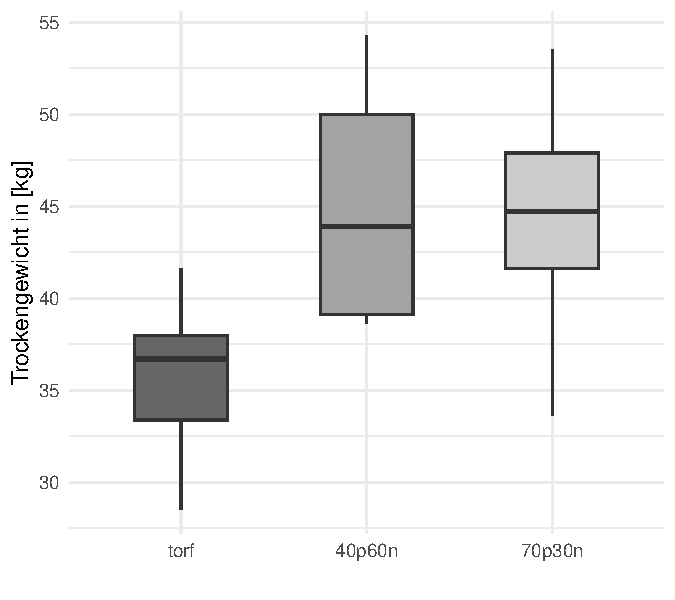
\includegraphics[width=\maxwidth]{img/boxplot-02-zer-1} 

}




Leider kennt sich Mark mit der Erstellung von Boxplots in \Rlogo nicht aus. Deshalb braucht er bei der Visualisierung Ihre Hilfe!

\begin{enumerate}
\item Erstellen Sie eine Tabelle mit den statistischen Maßzahlen aus der obigen Abbildung der drei Boxplots! \textit{Beachten Sie die korrekte Darstellungsform der statistischen Maßzahlen!} \textbf{(3 Punkte)}
\item Beschriften Sie \textit{einen} der Boxplots mit den gängigen statistischen Maßzahlen! \textbf{(2 Punkte)}
\item Erstellen Sie einen beispielhaften Datensatz, aus dem die drei Boxplots \textit{möglicherweise} erstellt wurden, im \Rlogo üblichen Format! \textbf{(2 Punkte)}
\item Kann Mark einen Unterschied zwischen den Behandlungen erwarten? Begründen Sie Ihre Antwort! \textbf{(2 Punkte)}
\end{enumerate} 
\clearpage
% -----------------------------------------------------------------------

\section{Aufgabe \hfill (9 Punkte)}

\textit{Geben Sie grundsätzlich Formeln und Rechenweg zur Lösung der Teilaufgaben mit an!} \\[1Ex]
 

 
%% --------------------------------------------------------------------
\begin{minipage}[t]{0.5\textwidth}

\includegraphics[width = 1.3cm]{/Users/kruppajo/work/GitHub/exam/avatare/Jonas.png}
\end{minipage}
\begin{minipage}[t]{0.5\textwidth}
\hfill
\href{https://youtu.be/0xc0jIPeiyw}{
\includegraphics[width = 2cm]{img/youtube}}
\end{minipage}
\vspace{-3ex}
%% --------------------------------------------------------------------



\paragraph{Visualisierung des Boxplots}

Jonas steht vor einem ersten Problem, denn wenn es nach seinem Betreuer geht, soll er in einem einem Freilandversuch Kartoffeln auswertet. Soweit eigentlich alles passend. Besser wäre was anderes gewesen. Jonas liebt Stricken. Darin kann er sich wirklich verlieren und immer wieder neu begeistern. Die Behandlung waren verschiedene Lüftungssystemen und Folientunneln ($ctrl$ und $tornado$). In seiner Exceldatei hat er den Messwert ($Y$) \textit{Frischegewicht} als \textit{freshmatter} aufgenommen. Nun soll Jonas die Daten eimal als Boxplots in einer Präsentation visualisieren, damit seinem Betreuer wieder klar wird, was er eigentlich nochmal gemacht hat und was für ein Ergbnis in einem statistischen Test zu erwarten wäre. Anhand von Boxplots lässt sich eine Aussage über die Varianzhomogenität über die Behandlungsgruppen treffen. Wäre da nicht noch etwas. Eine echte Herausforderung für ihn war schon immer die Erschöpfung gewesen. Ein leidiges Lied. Aber egal. Um zu Schwimmen geht Jonas dann später nochmal raus. Echte Entspannung.

\begin{table}[!h]
\centering
\begin{tabular}{cc}
\toprule
treatment & drymatter\\
\midrule
ctrl & 47.0\\
ctrl & 50.6\\
tornado & 35.1\\
ctrl & 48.2\\
tornado & 30.5\\
\addlinespace
ctrl & 72.0\\
tornado & 34.5\\
ctrl & 36.1\\
ctrl & 40.0\\
tornado & 32.0\\
\addlinespace
tornado & 40.8\\
tornado & 30.7\\
tornado & 31.9\\
ctrl & 39.4\\
ctrl & 53.6\\
\addlinespace
ctrl & 54.3\\
\bottomrule
\end{tabular}
\end{table}



Leider kennt sich Jonas mit der Erstellung von Boxplots nicht aus. Deshalb braucht er bei der Visualisierung Ihre Hilfe!

\begin{enumerate}
\item Zeichnen Sie in \textit{einer} Abbildung die beiden Boxplots für die zwei Behandlungen von Kartoffeln! Beschriften Sie die Achsen entsprechend! \textbf{(5 Punkte)} 
\item Wie ist Ihr Vorgehen, wenn Sie eine \textit{gerade} Anzahl an
  Beobachtungen pro Gruppe haben? \textbf{(1 Punkt)}
\item Beschriften Sie \textit{einen} der beiden Boxplots mit den gängigen
  statistischen Maßzahlen! \textbf{(2 Punkte)}
\item Wenn Sie \textit{keinen Effekt} zwischen den Behandlungen von
  Kartoffeln erwarten würden, wie sehen dann die beiden Boxplots aus?
  \textit{Antworten Sie mit einer Skizze der Boxplots!}
  \textbf{(1 Punkt)}
\end{enumerate} 
\clearpage
% -----------------------------------------------------------------------

\section{Aufgabe \hfill (8 Punkte)}

\textit{Geben Sie grundsätzlich Formeln und Rechenweg zur Lösung der Teilaufgaben mit an!} \\[1Ex]
 

 
%% --------------------------------------------------------------------
\begin{minipage}[t]{0.5\textwidth}

\includegraphics[width = 1.3cm]{/Users/kruppajo/work/GitHub/exam/avatare/Jonas.png}
\end{minipage}
\begin{minipage}[t]{0.5\textwidth}
\hfill
\href{https://youtu.be/aXvxGC4YLqk}{
\includegraphics[width = 2cm]{img/youtube}}
\end{minipage}
\vspace{-3ex}
%% --------------------------------------------------------------------



\paragraph{Visualisierung des Histogramm für kategoriale Daten}

'Hm...', Snickers und Iron Maiden. Das ist und bleibt die beste Kombination zum Nachdenken für Jonas. Jonas betrachtet die folgenden Daten nach einem Feldexperiment mit Lauch. In dem Experiment wurden die Knötchen gezählt. Nach der Meinung seinem Betreuer muss als erstes geschaut werden, wie diese verteilt sind. Also welcher statistischen Verteilung die Knötchen folgen. Dazu soll Jonas ein Histogramm verwenden. Dann hätte man auch einen guten Überblick über den Endpunkt ($Y$). Es wäre einfacher, wenn da nicht noch was wäre. Wenn die Erschöpfung nicht wäre, ja dann wäre wohl vieles möglich für Jonas! Aber so.. Wenn Iron Maiden ertönt, dann sucht das Meerschweinchen schleunigst Schutz unter dem Sofa. Jonas schüttelt den Kopf.

\begin{center}
Die Knötchen: 4, 6, 6, 4, 2, 1, 0, 7, 3, 8, 3, 3, 5, 2, 5, 5, 7, 3, 2, 4, 3, 7, 1, 3, 7, 5, 1, 6, 7, 7, 6, 3, 9
\end{center}

Leider kennt sich Jonas mit der Erstellung von Histogrammen überhaupt nicht aus. Deshalb braucht er bei der Erstellung Ihre Hilfe!

\begin{enumerate}
\item Zeichen Sie ein Histogramm um die Verteilung der Daten zu visualisieren! (\textbf{3 Punkte})
\item Beschriften Sie die Achsen der Abbildung! (\textbf{2 Punkte})
\item Ergänzen Sie die absoluten und relativen Häufigkeiten in der
  Abbildung! \textbf{(1 Punkt)}
\item Berechnen Sie aus den Daten die \textit{Wahrscheinlichkeit}
  mehr als die Anzahl 6 zu beobachten! \textbf{(1
    Punkt)}
\item Berechnen Sie aus den Daten die \textit{Chance} mehr
  als die Anzahl 6 zu beobachten! \textbf{(1 Punkt)}
\end{enumerate}

 
\clearpage
% -----------------------------------------------------------------------

\section{Aufgabe \hfill (8 Punkte)}

\textit{Geben Sie grundsätzlich Formeln und Rechenweg zur Lösung der Teilaufgaben mit an!} \\[1Ex]
 

 
%% --------------------------------------------------------------------
\begin{minipage}[t]{0.5\textwidth}

\includegraphics[width = 1.3cm]{/Users/kruppajo/work/GitHub/exam/avatare/Tina.png}
\end{minipage}
\begin{minipage}[t]{0.5\textwidth}
\hfill
\href{https://youtu.be/ORHSPTCdfeY}{
\includegraphics[width = 2cm]{img/youtube}}
\end{minipage}
\vspace{-3ex}
%% --------------------------------------------------------------------



\paragraph{Visualisierung des Histogramm für kontinuierliche Daten}

In einem Gespräch mit ihrer Betreuerin wird Tina gebeten seine Daten aus einem Kreuzungsexperiment mit Schweinen in einem Histogramm darzustellen. Aus den Boxen wummert Tocotronic und ihr Mund ist verklebt von Katjes. 'Herrlich', denkt Tina. In ihrem Experiment hat er die mittlere Anzahl an weißen Blutkörperchen erst fotographiert und dann ausgezählt. Laut ihrer Betreuerin soll das Histogramm helfen, die Verteilung der die mittlere Anzahl an weißen Blutkörperchen zu bestimmen.  Es wäre einfacher, wenn da nicht noch was wäre. Wenn die Wut nicht wäre, ja dann wäre wohl vieles möglich für Tina! Aber so.. Wenn Tocotronic ertönt, dann sucht die Spinne schleunigst Schutz unter dem Sofa. Tina schüttelt den Kopf.

\begin{center}
Die mittlere Anzahl an weißen Blutkörperchen: 8, 12, 11.5, 12.5, 11.5, 11.3, 8.9, 12.6, 3.9, 13.9, 13.4, 9.7, 6.6, 12.4, 11.1, 12.9, 5.9, 10.3, 7, 10, 10.4, 6.5
\end{center}

Leider kennt sich Tina mit der Erstellung von Histogrammen überhaupt nicht aus. Deshalb braucht sie bei der Erstellung Ihre Hilfe!

\begin{enumerate}
\item Zeichen Sie ein Histogramm um die Verteilung der Daten zu visualisieren! (\textbf{3 Punkte})
 \item Erläutern Sie Ihr Vorgehen um ein Histogramm für kontinuierliche Daten zu zeichnen!  (\textbf{2 Punkte})
\item Beschriften Sie die Achsen der Abbildung! (\textbf{2 Punkte})
\item Ergänzen Sie die relativen Häufigkeiten in der Abbildung! \textbf{(1 Punkt)}  
\end{enumerate}

 
\clearpage
% -----------------------------------------------------------------------

\section{Aufgabe \hfill (10 Punkte)}

\textit{Geben Sie grundsätzlich Formeln und Rechenweg zur Lösung der Teilaufgaben mit an!} \\[1Ex]
 

 
%% --------------------------------------------------------------------
\begin{minipage}[t]{0.5\textwidth}

\includegraphics[width = 1.3cm]{/Users/kruppajo/work/GitHub/exam/avatare/Mark.png}
\end{minipage}
\begin{minipage}[t]{0.5\textwidth}
\hfill
\href{https://youtu.be/VAqiUdV4WQ0}{
\includegraphics[width = 2cm]{img/youtube}}
\end{minipage}
\vspace{-3ex}
%% --------------------------------------------------------------------




\paragraph{Visualisierung des Scatterplots}

Mark liest laut: 'Wenn zwei kontinuierliche Variablen vorliegen, können diese in einer exploartiven Datenanalyse...'. Mark stoppt. Mark schmeißt noch eine Handvoll Marzipankugeln in seinen Rachen. Im Hintergrund klirrt leise der Spiegel zum Sound von Andrea Berg. Was waren noch gleich kontinuierliche Variablen? In seiner Hausarbeit hatte er ein Freilandversuch im Teuteburgerwald durchgeführt. Dabei ging es um den Zusammenhang zwischen Chlorophyllgehalt (SPAD-502Plus) [SPAD] und durchschnittlichen Anteil an Ton [\%/l] im groben Kontext von Erbsen. Nun stellt sich die Frage für ihn, ob es überhaupt einen Zusammenhang zwischen den gemessenen Variablen gibt. Dafür war eine explorative Datenanalyse gut! Wenn die Unsicherheit nicht wäre, ja dann wäre wohl vieles möglich für Mark! Aber so.. Dann was anderes. Wenn Columbo läuft, dann ist der Hamster nicht mehr da. Aber jetzt braucht er mal Entspannung!

\begin{table}[!h]
\centering
\begin{tabular}{cc}
\toprule
Chlorophyllgehalt (SPAD-502Plus) [SPAD] & Durchschnittlichen Anteil an Ton [\%/l]\\
\midrule
18.1 & 31.6\\
10.8 & 18.8\\
12.3 & 20.5\\
12.3 & 23.5\\
19.0 & 25.1\\
\addlinespace
13.6 & 24.2\\
17.9 & 26.6\\
13.0 & 21.3\\
10.2 & 17.6\\
17.2 & 24.9\\
\addlinespace
15.0 & 26.6\\
\bottomrule
\end{tabular}
\end{table}



Leider kennt sich Mark mit der Erstellung einer explorativen Datenanalyse für kontinuierliche Daten überhaupt nicht aus. Deshalb braucht er bei der Erstellung Ihre Hilfe!

\begin{enumerate}
\item Erstellen Sie eine Visualisierung für die Datentabelle. Beschriften Sie
  die Achsen entsprechend! \textbf{(4 Punkte)}
\item Schätzen Sie eine Gerade durch die Punkte! \textbf{(1 Punkt)}
\item Beschriften Sie die Gerade mit den gängigen statistischen Maßzahlen! Geben Sie die numerischen Zahlenwerte mit an! \textbf{(3 Punkte)}
\item Wenn \textit{kein} Effekt von $x$ auf $y$ vorhanden wäre, wie würde die Gerade verlaufen und welche Werte würden die statistischen Maßzahlen annehmen? \textbf{(2 Punkt)}
\end{enumerate} 
\clearpage
% -----------------------------------------------------------------------

\section{Aufgabe \hfill (10 Punkte)}

\textit{Geben Sie grundsätzlich Formeln und Rechenweg zur Lösung der Teilaufgaben mit an!} \\[1Ex]
 

 
%% --------------------------------------------------------------------
\begin{minipage}[t]{0.5\textwidth}

\includegraphics[width = 1.3cm]{/Users/kruppajo/work/GitHub/exam/avatare/Yuki.png}
\end{minipage}
\begin{minipage}[t]{0.5\textwidth}
\hfill
\href{https://youtu.be/t_1KL77mfmg}{
\includegraphics[width = 2cm]{img/youtube}}
\end{minipage}
\vspace{-3ex}
%% --------------------------------------------------------------------



\paragraph{Visualisierung des Mosaicplots}

Irgendwie komisch, wenn sie Matrix anmacht, dann ist das Minischwein eigentlich sofort vor dem Bildschirm und starrt hinein. Aber Ablenkung hilft nur begrenzt. 'Uff!', denkt sich Yuki. Jetzt hat sie doch tatsächlich zwei kategoriale Variablen in ihrer Hausarbeit gemessen. Zum einen die Behandlung Klimakontrolle [ja/nein] und zum anderen die Messung Fettgehalt erreicht [ja/nein] im Kontext von Zandern. Hierfür hat sie ein Stallexperiment im Emsland durchgeführt. Jetzt möchte Yuki die Daten einmal in einer explorativen Datenanalyse darstellen. Danach kann sie dann über den passenden statistischen Test nachdenken. Dabei unterstützt ihre Betreuerin diesen Ansatz bevor es in der Datenanalyse weiter geht. So schön wie so gut. Wenn die Faulheit nicht wäre, ja dann wäre wohl vieles möglich für Yuki! Aber so..



\vspace{1Ex}

\begin{center}
\begin{minipage}[t]{0.45\textwidth}
%\small
\begin{center}

\begin{tabular}{p{2.5cm}p{2.5cm}p{2.5cm}p{2.5cm}}
\toprule
Fettgehalt erreicht & Klimakontrolle\\
\midrule
nein & ja\\
nein & ja\\
nein & ja\\
ja & ja\\
nein & ja\\
\addlinespace
nein & nein\\
ja & nein\\
nein & ja\\
ja & nein\\
nein & ja\\
\addlinespace
ja & nein\\
ja & nein\\
ja & nein\\
nein & ja\\
nein & ja\\
\bottomrule
\end{tabular}


\end{center}
\end{minipage}
\begin{minipage}[t]{0.45\textwidth}
%\small
\begin{center}

\begin{tabular}{p{2.5cm}p{2.5cm}p{2.5cm}p{2.5cm}}
\toprule
Fettgehalt erreicht & Klimakontrolle\\
\midrule
ja & nein\\
ja & nein\\
nein & ja\\
nein & ja\\
ja & nein\\
\addlinespace
ja & nein\\
nein & nein\\
nein & ja\\
ja & nein\\
ja & nein\\
\addlinespace
nein & nein\\
nein & ja\\
nein & ja\\
ja & ja\\
ja & ja\\
\bottomrule
\end{tabular}


\end{center}
\end{minipage}
\end{center}

\vspace{2Ex}

Leider kennt sich Yuki mit der Erstellung einer explorativen Datenanalyse für kategoriale Daten überhaupt nicht aus. Deshalb braucht sie bei der Erstellung Ihre Hilfe!

\begin{enumerate}
\item Stellen Sie den Zusammenhang zwischen den beiden kategorialen Variablen in einer zusammenfassenden Tabelle dar! \textbf{(3 Punkte)}
\item Visualisieren Sie den Zusammenhang zwischen den beiden kategorialen Variablen! \textbf{(3 Punkte)}
\item Berechnen Sie die Verhältnisse in der Visualisierung! Welche Annahme haben Sie getroffen? \textbf{(2 Punkte)}
\item Wenn \textit{ein} Effekt von der Behandlung vorliegen würde, wie würde die Tabelle und die Visualisierung aussehen? \textbf{(2 Punkt)}
\end{enumerate} 
\clearpage
% -----------------------------------------------------------------------

\section{Aufgabe \hfill (10 Punkte)}

\textit{Geben Sie grundsätzlich Formeln und Rechenweg zur Lösung der Teilaufgaben mit an!} \\[1Ex]
 

 
%% --------------------------------------------------------------------
\begin{minipage}[t]{0.5\textwidth}

\includegraphics[width = 1.3cm]{/Users/kruppajo/work/GitHub/exam/avatare/Jessica.png}\hspace{-4mm}
\includegraphics[width = 1.3cm]{/Users/kruppajo/work/GitHub/exam/avatare/Nilufar.png}
\end{minipage}
\begin{minipage}[t]{0.5\textwidth}
\hfill
\href{https://youtu.be/Op-gjzASH9I}{
\includegraphics[width = 2cm]{img/youtube}}
\end{minipage}
%% --------------------------------------------------------------------



\paragraph{Visualisierung von Verteilungen}

'Was soll das denn jetzt schon wieder sein? Drei Boxplot, die auf der Seite liegen?', entfährt es Nilufar und schaut dabei Jessica an. 'Keine Ahnung. Es ist bestimmt wieder so ein Lernziel mit der Verteilung und so.', meint Jessica sichtlich genervt und mampft noch ein paar Schokobons. 'Du weißt doch wie es heißt, \textit{Frei ist, wer missfallen kann.}\footnote{Oschmann, A. (2024) Mädchen stärken: Stärken fördern, Selbstwert erhöhen und liebevoll durch Krisen begleiten. Goldegg Verlag}', merkt Nilufar nickend an. Die beiden schauen angestrengt auf die drei Boxplots. Das Ziel ist es zu verstehen, wie eine Verteilung anhand eines Boxplots bewertet werden kann. Jessica und der Mangel machen die Sache nicht einfacher.



{\centering 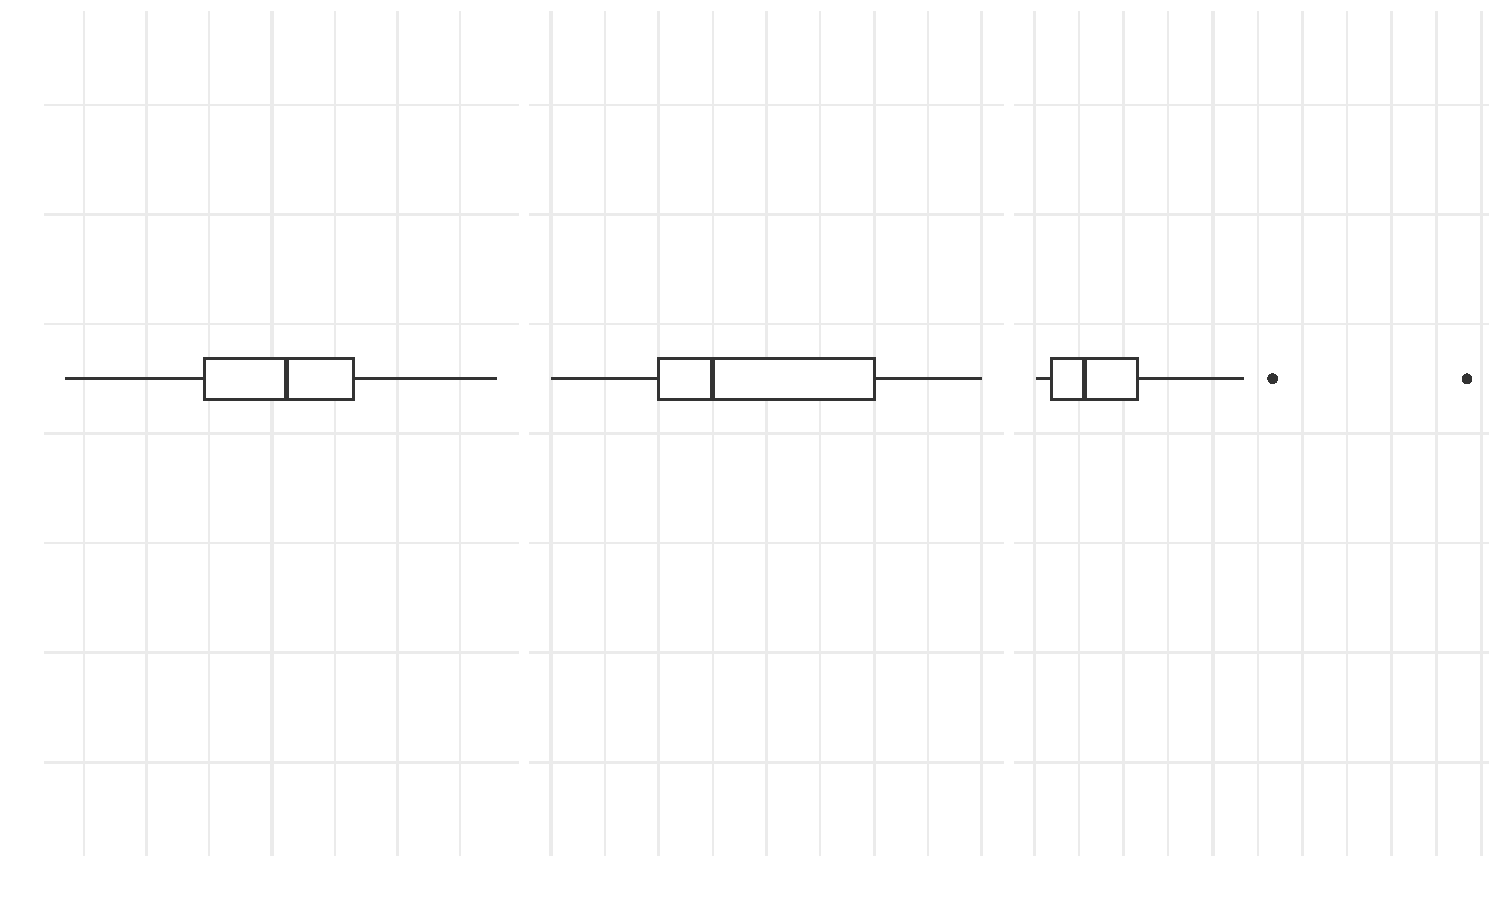
\includegraphics[width=\maxwidth]{img/desc-stat-11-1} 

}




Jetzt brauchen Nilufar und Jessica Ihre Hilfe bei der Abschätzung einer Verteilung anhand von Boxplots um ihre Arbeit dann in diesem Semester noch abschließen zu können.

\begin{enumerate}
\item Zeichnen Sie über die Boxplots die entsprechende zugehörige Verteilung! \textbf{(3 Punkte)} 
\item Zeichnen Sie unter die Boxplots die entsprechende zugehörige Beobachtungen als Stiche! \textbf{(3 Punkte)}
\item Wie viel Prozent der Beobachtungen fallen in das IQR? Ergänzen Sie die Abbildung entsprechend um den Bereich! \textbf{(2 Punkte)}
\item Wie viel Prozent der Beobachtungen fallen in $\bar{y} \pm 1s$ und $\bar{y} \pm 2s$  unter der Annahme einer Normalverteilung? \textbf{(2 Punkte)}
\end{enumerate} 
\clearpage
% -----------------------------------------------------------------------

\section{Aufgabe \hfill (10 Punkte)}

\textit{Geben Sie grundsätzlich Formeln und Rechenweg zur Lösung der Teilaufgaben mit an!} \\[1Ex]
 

 
%% --------------------------------------------------------------------
\begin{minipage}[t]{0.5\textwidth}

\includegraphics[width = 1.3cm]{/Users/kruppajo/work/GitHub/exam/avatare/Alex.png}\hspace{-4mm}
\includegraphics[width = 1.3cm]{/Users/kruppajo/work/GitHub/exam/avatare/Paula.png}
\end{minipage}
\begin{minipage}[t]{0.5\textwidth}
\hfill
\href{https://youtu.be/ZrJhn2wPbq4}{
\includegraphics[width = 2cm]{img/youtube}}
\end{minipage}
%% --------------------------------------------------------------------



\paragraph{Visualisierung der Normalverteilung}

'Jetzt haben wir schon überall geschaut und ich finde die verdammte die Ratte nicht. Wo ist die den normalerweise? Und wenn du jetzt einen blöden Witz über die Aufgabe und normal machst, dann gehe ich.', faucht Paula Alex an. 'Ui, alles gut. Vielleicht ein paar Gummibärchen zur Entspannung?', entgegnet Alex. Manchmal macht der Perfektionismus Paula zu einem anderen Menschen, der sie nicht sein will. Da rennt dann auch die Ratte vor ihr weg. Jetzt sollen die beiden diese Aufgabe zur Normalverteilung lösen. Es geht um verschiedene Normalverteilungen udn zu verstehen, wie die Parameter der Normalverteilung funktionieren. Anscheinend hängen Normalverteilungen vom Mittelwert $\bar{y}$ und der Standardabweichung $s$ ab.\\



Jetzt brauchen Paula und Alex Ihre Hilfe bei der Abschätzung einer Verteilung um ihre Arbeit dann in diesem Semester noch abschließen zu können.

\begin{enumerate}
\item Skizzieren Sie zwei Normalverteilungen mit $\bar{y}_1 \neq \bar{y}_2$ und $s_1 \neq s_2$! \textbf{(3 Punkte)}
\item Beschriften Sie die Normalverteilungen mit den statistischen Maßzahlen! \textbf{(2 Punkte)}
\item Liegt Varianzhomogenität oder Varianzheterogenität vor? Begründen Sie Ihre Antwort! \textbf{(2 Punkte)}
\item In welchen Bereich fallen 68\% bzw. 95\% der Beobachtungen in einer Normalverteilung? Ergänzen Sie die Bereiche in \underline{einer} Normalverteilung! \textbf{(2 Punkte)}
\item Ergänzen Sie unter \underline{einer} der Normalverteilungen den entsprechenden Boxplot! \textbf{(1 Punkt)}
\end{enumerate}

 
\clearpage
% -----------------------------------------------------------------------

\section{Aufgabe \hfill (10 Punkte)}

\textit{Geben Sie grundsätzlich Formeln und Rechenweg zur Lösung der Teilaufgaben mit an!} \\[1Ex]
 

 
%% --------------------------------------------------------------------
\begin{minipage}[t]{0.5\textwidth}

\includegraphics[width = 1.3cm]{/Users/kruppajo/work/GitHub/exam/avatare/Jessica.png}\hspace{-4mm}\includegraphics[width = 1.3cm]{/Users/kruppajo/work/GitHub/exam/avatare/Paula.png}
\end{minipage}
\begin{minipage}[t]{0.5\textwidth}
\hfill
\href{https://youtu.be/MiD42k4l5Ag}{\includegraphics[width = 2cm]{img/youtube}}
\end{minipage}
%% --------------------------------------------------------------------



\paragraph{Visualisierung der Normalverteilung und der Poissonverteilung}

'Wer hat sich denn sowas ausgedacht? Verteilungen?', entfährt es Paula und schaut dabei Jessica an. In ihrer Hand zerdrückt sie Schokobons von Jessica. 'Wir sollen eine Normalverteilung mit einem Mittelwert von $\bar{y}_1 = 2$ und einer Standardabweichung von $s_1 = 1$ zeichnen. Sowie eine weitere Normalverteilung mit einem Mittelwert von $\bar{y}_2 = 0$ und einer Standardabweichung von $s_2 = 1$. Keine Ahnung wie das geht. Darunter sollen dann noch eine Poissonverteilung mit einem Mittelwert von $\lambda_1 = 2$ sowie einer weiteren Poissonverteilung mit einem Mittelwert von $\lambda_2 = 20$ gezeichnet werden.', meint Jessica sichtlich eingeschüchtert und rettet noch ein paar Schokobons in seinem Mund. Paula und der Perfektionismus machen die Suche nach der Lösung nicht einfacher. Im Hintergrund spielt viel zu laut David Bowie, die diesmal Paula ausgewählt hat und die Ratte schon in die Küche vertrieben hat, wo es den Biomüll mampft.\\




{\centering \includegraphics[width=\maxwidth]{img/histogram-01-1} 

}




Jetzt brauchen Paula und Jessica Ihre Hilfe bei der Abschätzung einer Verteilung um ihre Arbeit dann in diesem Semester noch abschließen zu können.


\begin{enumerate}
\item Skizzieren Sie die zwei Normalverteilungen und zwei Poissonverteilungen! \textbf{(4 Punkte)}
\item Achten Sie auf die entsprechende Skalierung in den jeweiligen Abbildungen! \textbf{(2 Punkte)}
\item Ergänzen Sie unter \underline{einer} Normalverteilung den entsprechenden Boxplot! \textbf{(1 Punkt)}
\item Ergänzen Sie unter \underline{einer} Poissonverteilung den entsprechenden Boxplot! \textbf{(1 Punkt)}
\item Geben Sie ein Beispiel für ein Outcome $y$, welches einer Normalverteilung folgt! \textbf{(1 Punkt)}
\item Geben Sie ein Beispiel für ein Outcome $y$, welches einer Poissonverteilung folgt! \textbf{(1 Punkt)}
\end{enumerate} 
\clearpage
% -----------------------------------------------------------------------
\part{Statistisches Testen \& statistische Testtheorie}
% -----------------------------------------------------------------------  

\section{Aufgabe \hfill (9 Punkte)}


 
%% --------------------------------------------------------------------
\begin{minipage}[t]{0.5\textwidth}
\includegraphics[width = 1.3cm]{/Users/kruppajo/work/GitHub/exam/avatare/Mark.png}\hspace{-4mm}\includegraphics[width = 1.3cm]{/Users/kruppajo/work/GitHub/exam/avatare/Yuki.png}
\end{minipage}
\begin{minipage}[t]{0.5\textwidth}
\hfill
\href{https://youtu.be/aHVYuFKTqZs}{\includegraphics[width = 2cm]{img/youtube}}
\end{minipage}
%% --------------------------------------------------------------------



\paragraph{Grundgesamtheit und experimentelle Stichprobe}

'Schnapspraline?', räuspert sich das Känguruh und schaukelt in der Wippe. Mark und Yuki schauen erschrocken auf. 'Ähm, das ist hier eine Klausuraufgabe...', merkt Mark mit leicht schrägen Blick an. 'Ich mache hier ein Praktikum und schreibe Teile der Aufgaben.', gähnt das Känguruh. 'Also, ich glaube das ist so nicht gedacht. Und das sind die Schnapspralinen für den Geburtstag meiner Oma!', ruft Yuki. 'Pillepalle! Meins, deins, das sind doch alles bürgerliche Kategorien!', entgegnet das Känguruh und liest von einem zerknitterten Stück Papier ab: 'Was ist der Unterschied zwischen dem Einen und dem Anderen. Steht alles unten in den Fragen. Einfach selber lesen...'.

\vspace{1ex}

Leider kennen sich Mark und Yuki mit der Grundgesamtheit und der Stuchprobe überhaupt nicht aus. Daher sind Sie gefragt!

\begin{enumerate}
\item Nennen Sie das statistische Verfahren und zwei konkrete Beispiele zur Durchführung um von einer Grundgesamtheit auf eine Stichprobe zu gelangen! \textbf{(3 Punkte)}
\item Erklären Sie den Zusammenhang zwischen Stichprobe und Grundgesamtheit an einem Schaubild! Beschriften Sie das Schaubild entsprechend!
  \textit{Nutzen Sie hierfür als Veranschaulichung die Körpergröße von Männern oder Frauen aus den Gummibärchendaten!}  \textbf{(3 Punkte)}
\item Erweitern Sie das Schaubild um die Entstehung von $Pr(D|H_0)$! \textit{Nutzen Sie hierfür als Veranschaulichung zusätzlich die Gruppierungsvariable "`Modul"' aus den Gummibärchendaten!}  \textbf{(3 Punkte)}
\end{enumerate} 
\clearpage
% -----------------------------------------------------------------------

\section{Aufgabe \hfill (9 Punkte)}


 
%% --------------------------------------------------------------------
\begin{minipage}[t]{0.5\textwidth}
\includegraphics[width = 1.3cm]{/Users/kruppajo/work/GitHub/exam/avatare/Nilufar.png}\hspace{-4mm}\includegraphics[width = 1.3cm]{/Users/kruppajo/work/GitHub/exam/avatare/Paula.png}
\end{minipage}
\begin{minipage}[t]{0.5\textwidth}
\hfill
\href{https://youtu.be/Ric8ne39DtI}{\includegraphics[width = 2cm]{img/youtube}}
\end{minipage}
%% --------------------------------------------------------------------



\paragraph{Das Nullritual - Die statistische Testtheorie}

'Fechten ist der beste Sport, den es gibt.', meint Paula. Nilufar entgegnet, ' Ich empfehle ja immer allen Kicken.' Die beiden sind im Zoo und diskutieren, ob Pinguine Knie haben. Eigentlich wollten beide nochmal die statistische Testheorie durchgehen, sind dann aber auf abenteuerlichen Wege im Zoo gelandet. Paula starrt wie hypnotisiert auf einen strullenden Elefanten und stopt die Zeit.\footnote{Yang, P. J., et al. (2014). Duration of urination does not change with body size. Proceedings of the National Academy of Sciences, 111(33), 11932-11937.} 'Du bist so peinlich.', entfährt es Nilufar.

\vspace{1ex}

Leider kennen sich Paula und Nilufar mit statistischen Testtheorie, auch Null-Ritual genannt, überhaupt nicht aus. Geschweige denn mit der Visualisierung als Kreuztabelle.  

\begin{enumerate}
\item Tragen Sie folgende statistische Fachbegriffe zur statistischen Testtheorie korrekt eine selbst erstellte Kreuztabelle ein! \textbf{(3 Punkte)}
  \begin{center}
  \begin{tabular}{cccc}
  20\% & Testentscheidung & 5\% & Richtige Entscheidung \\
  \end{tabular}
  \end{center}
\item Ergänzen Sie Ihre erstellte Kreuztabelle um vier weitere, passende Fachbegriffe zur statistischen Testtheorie! \textbf{(2 Punkte)}
\end{enumerate}

Die Entscheidungsfindung durch einen statistischen Test kann auch durch die Analogie zu einem Feuermelder abgebildet werden. Dabei symbolisiert der Feuermelder den statistischen Test und es soll getestet werden, ob ein Feuer ausgebrochen ist.

\begin{enumerate}
  \setcounter{enumi}{2}    
\item In der Analogie des Feuermelders, wie lautet der $\alpha$-Fehler? \textbf{(1 Punkt)}
\item In der Analogie des Feuermelders, wie lautet der $\beta$-Fehler? \textbf{(1 Punkt)}
\item Wenn der Feuermelder einmal pro Tag messen würde, wie oft würde der Feuermelder mit einem $\alpha$ von 5\% in einem Jahr Alarm schlagen? Begründen Sie Ihre Antwort! \textbf{(2 Punkte)}
\end{enumerate}



 
\clearpage
% -----------------------------------------------------------------------

\section{Aufgabe \hfill (9 Punkte)}

\textit{Geben Sie grundsätzlich Formeln und Rechenweg zur Lösung der Teilaufgaben mit an!} \\[1Ex]


 
%% --------------------------------------------------------------------
\begin{minipage}[t]{0.5\textwidth}
\includegraphics[width = 1.3cm]{/Users/kruppajo/work/GitHub/exam/avatare/Nilufar.png}\hspace{-4mm}\includegraphics[width = 1.3cm]{/Users/kruppajo/work/GitHub/exam/avatare/Yuki.png}
\end{minipage}
\begin{minipage}[t]{0.5\textwidth}
\hfill
\href{https://youtu.be/32JjH1eyuTU}{\includegraphics[width = 2cm]{img/youtube}}
\end{minipage}
%% --------------------------------------------------------------------



\paragraph{Visualisierung der Teststatistik $\boldsymbol{T_D}$ und dem p-Wert}

'Kannst du mir nochmal an einer Visualisierung erklären, wie der Zusammenhang zwischen der Teststatistik aus den Daten $T_D$ und dem p-Wert ist? Ich habe hier zig Fachbegriffe, kriege die abr nicht zusammen...', fragt Yuki nachdrücklich  Nilufar. Das hilft aber nur bedingt, denn Nilufar hat wenig geschlafen und träumt zu den Klängen von London Grammar. Yuki hatte den ganzen Abend mit Nilufar über die Faulheit diskutiert und nun sind beide voll neben der Spur. So wird es nichts mit der Klausur. Yuki mampft noch ein paar Reese's Peanut Butter Cups und nickt ein. Jetzt brauchen die beiden gesondert Hilfe!

\vspace{1ex}

Leider kennen sich Yuki und Nilufar mit der Visualisierung der Teststatistik $T_D$ und dem p-Wert überhaupt nicht aus und brauchen dahr Ihre Hilfe!

\vspace{1ex}

\textit{Beachten Sie, dass im Folgenden \underline{keine numerisch korrekte Darstellung} verlangt wird! Es gilt Erkennbarkeit vor Genauigkeit!}

\begin{enumerate}
\item Ergänzen Sie eine beschriftete $x$-Achse! \textbf{(1 Punkt)}
\item Ergänzen Sie "`$\bar{y}_1 = \bar{y}_2$"'! \textbf{(1 Punkt)} 
\item Ergänzen Sie "`$A = 0.95$"'! \textbf{(1 Punkt)}
\item Zeichnen Sie $T_{\alpha=5\%}$ in die Abbildung! \textbf{(1 Punkt)} 
\item Zeichnen Sie das Signifikanzniveau $\alpha$ in die Abbildung! Begründen Sie Ihre Antwort! \textbf{(2 Punkte)} 
\item Zeichnen Sie $-T_{D}$ in die Abbildung! \textbf{(1 Punkt)}
\item Zeichnen Sie einen signifikant p-Wert in die Abbildung! Begründen Sie Ihre Antwort! \textbf{(2 Punkte)}   
\end{enumerate}



{\centering \includegraphics[width=\maxwidth]{img/statistisches-testen-3-1} 

}


 
\clearpage
% -----------------------------------------------------------------------

\section{Aufgabe \hfill (10 Punkte)}


 
%% --------------------------------------------------------------------
\begin{minipage}[t]{0.5\textwidth}
\includegraphics[width = 1.3cm]{/Users/kruppajo/work/GitHub/exam/avatare/Jonas.png}\hspace{-4mm}\includegraphics[width = 1.3cm]{/Users/kruppajo/work/GitHub/exam/avatare/Tina.png}
\end{minipage}
\begin{minipage}[t]{0.5\textwidth}
\hfill
\href{https://youtu.be/CN_O4fYPbhs}{\includegraphics[width = 2cm]{img/youtube}}
\end{minipage}
%% --------------------------------------------------------------------



\paragraph{Visualisierung des 95\% Konfidenzintervalls}

'So, was haben wir gemacht? Wir haben einen t-test für den Vergleich der Mittelwerte gerechnet.', meint Jonas. Tina schaut fragend. 'Hatten wir nicht alles zu einer Kontrolle verglichen? Das war doch so!', ruft Tina laut aus. 'Wir haben doch als Messwert \textit{Energieverbrauch der Klimakammer} erhoben.', stellt Jonas fest. Jetzt haben beide das Problem, die möglichen 95\% Konfidenzintervalle zu interpretieren.

\vspace{1ex}

Leider kennen sich Jonas und Tina mit der Visualisierung des 95\% Konfidenzintervall überhaupt nicht aus. 

\begin{enumerate}
\item Beschriften Sie die untenstehende Abbildung mit der Signifikanzschwelle! Begründen Sie Ihre Antwort! \textbf{(2 Punkte)}
\item Ergänzen Sie eine \textit{in den Kontext passende} Relevanzschwelle! Begründen Sie Ihre Antwort! \textbf{(2 Punkte)} 
\item Skizieren Sie in die untenstehende Abbildung sechs einzelne Konfidenzintervalle (a-f) mit den
  jeweiligen Eigenschaften! \textbf{(6 Punkte)}
  \begin{itemize}
  \item[(a)] Ein 95\% Konfidenzintervall mit h{"o}herer Varianz $s_p$ in der Stichprobe als der Rest der 95\% Konfidenzintervalle 	
  \item[(b)] Ein nicht signifikantes, nicht relevantes 95\% Konfidenzintervall 	
  \item[(c)] Ein signifikantes, relevantes 95\% Konfidenzintervall 	
  \item[(d)] Ein signifikantes, relevantes 99\% Konfidenzintervall. 
  \item[(e)] Ein 95\% Konfidenzintervall mit niedriger Varianz $s_p$ in der Stichprobe als der Rest 95\% der Konfidenzintervalle
  \item[(f)] Ein signifikantes, nicht relevantes 95\% Konfidenzintervall
  \end{itemize}
\end{enumerate}

\begin{center}
  \includegraphics[height = 10cm]{/Users/kruppajo/work/GitHub/exam/question/img/statistisches-testen-04}
\end{center}


 
\clearpage
% -----------------------------------------------------------------------

\section{Aufgabe \hfill (10 Punkte)}

\textit{Geben Sie grundsätzlich Formeln und Rechenweg zur Lösung der Teilaufgaben mit an!} \\[1Ex]


 
%% --------------------------------------------------------------------
\begin{minipage}[t]{0.5\textwidth}
\includegraphics[width = 1.3cm]{/Users/kruppajo/work/GitHub/exam/avatare/Nilufar.png}\hspace{-4mm}\includegraphics[width = 1.3cm]{/Users/kruppajo/work/GitHub/exam/avatare/Steffen.png}
\end{minipage}
\begin{minipage}[t]{0.5\textwidth}
\hfill
\href{https://youtu.be/FgZmpnEWDag}{\includegraphics[width = 2cm]{img/youtube}}
\end{minipage}
%% --------------------------------------------------------------------



\paragraph{Zusammenhang zwischen dem Effekt, der Streuung sowie der Fallzahl}

An einem heißen Juliabend haben sich Nilufar und Steffen zum Lernen verabredet. Eine große Kanne Eistee und Berge von Takis Blue Heat schmelzen in der Sonne  und warten darauf gegessen zu werden. Nilufar liest laut vor:\begin{quote}
                 \textit{
                 Beim statistischen Testen gibt es einen Zusammenhang zwischen dem Effekt, der Streuung sowie der Fallzahl. Gegeben sei die Formel für den Student t-Test auf den die folgenden Überlegungen basieren sollen. Welche Auswirkung hat die Änderungen der jeweiligen statistischen Maßzahl des Effekts $\Delta$, der Streuung $s$ und der Fallzahl $n$ auf die Teststistik $T_{D}$, den p-Wert $Pr(D|H_0)$ sowie dem Konfidenzintervall $KI_{1-\alpha}$?
                 }
                 \end{quote}Steffen hebt die Augenbraue. 'Ich bleibe dabei. Wir sollten erstmal Harry Potter schauen, bis es kühler ist. Den Film habe ich doch extra mitgebracht!' Nilufar ist der Idee nicht abgeneigt und auch das Huhn kommt auf die Terasse um dabei zu sein.

\vspace{1ex}

Leider kennen sich Nilufar und Steffen mit dem Zusammenhang zwischen dem Effekt, der Streuung sowie der Fallzahl überhaupt nicht aus. 


\begin{enumerate}
\item Visualisieren Sie den Zusammenhang zwischen der Teststatiatik $T_{D}$ und dem p-Wert $Pr(D|H_0)$ für sich verändernde $T_{D}$-Werte!\textit{Geben Sie dafür ein numerisches Beispiel in dem Sie drei $T_{D}$-Werte und deren Einfluss auf den p-Wert vergleichen!} \textbf{(3 Punkte)}  
\item  Füllen Sie die untenstehende Tabelle aus in dem Sie die Änderung der statistischen Maßzahlen auf die Teststatistik, den p-Wert sowie das Konfidenzintervall in \textit{einem} Wort oder Symbol beschreiben! \textbf{(4 Punkte)}
\begin{center}
  \large
  \begin{tabular}[c]{l|c|c|c|l|c|c|c}
    & $T_{D}$ & $Pr(D|H_0)$ & $KI_{1-\alpha}$ & & $T_{D}$ & $Pr(D|H_0)$ & $KI_{1-\alpha}$\strut\\ 
    \hline
    \textbf{$\Delta\; \uparrow$} & \hspace{1.8cm} & \hspace{1.8cm}  & \hspace{1.8cm} & \textbf{
                                                          $\Delta\; \downarrow$} &
                                                                          \hspace{1.8cm} & \hspace{1.8cm}  & \hspace{1.8cm}\strut\\
    \hline
        \textbf{$s\; \uparrow$} & \hspace{1.8cm} & \hspace{1.8cm}  & \hspace{1.8cm} & \textbf{
                                                          $s\; \downarrow$} &
                                                                          \hspace{1.8cm}
                                                & \hspace{1.8cm}  & \hspace{1.8cm}\strut\\
    \hline
        \textbf{$n\; \uparrow$} & \hspace{1.8cm} & \hspace{1.8cm}  & \hspace{1.8cm} & \textbf{
                                                          $n\; \downarrow$} &
                                                                          \hspace{1.8cm}
                                                & \hspace{1.8cm}  & \hspace{1.8cm}\strut\\
    \hline
  \end{tabular}
\end{center}
\item Visualisieren Sie ein 95\%-iges Konfidenzintervall im Vergleich zu einem 99\%-igen Konfidenzintervall! Begründen Sie Ihre Visualisierung anhand der Formel des Konfidenzintervalls des t-Tests mathematisch! \textbf{(3 Punkte)} 
\end{enumerate} 
\clearpage
% -----------------------------------------------------------------------
\part{Der Student t-Test, Welch t-Test \& gepaarter t-Test}
% -----------------------------------------------------------------------

\section{Aufgabe \hfill (9 Punkte)}

\textit{Geben Sie grundsätzlich Formeln und Rechenweg zur Lösung der Teilaufgaben mit an!} \\[1Ex]
 

 
%% --------------------------------------------------------------------
\begin{minipage}[t]{0.5\textwidth}
\includegraphics[width = 1.3cm]{/Users/kruppajo/work/GitHub/exam/avatare/Nilufar.png}
\end{minipage}
\begin{minipage}[t]{0.5\textwidth}
\hfill
\href{https://youtu.be/eejS2uG4o-M}{\includegraphics[width = 2cm]{img/youtube}}
\end{minipage}
\vspace{-3ex}
%% --------------------------------------------------------------------



\paragraph{Berechnung des Student t-Test \underline{oder} Welch t-Test}

Nilufar ist im Wendland für einen Pilotexperiment mit sehr geringer Fallzahl $(n_1 = n_2 = 3)$ mit Fleischrindern. Allein diese Tatsache ist für sie eine Erzählung wert. Eine echte Herausforderung für sie war schon immer die Erwartung gewesen. Ein leidiges Lied.  Für ihre Abschlussarbeit musste sie ein Stallexperiment mit Fleischrindern durchführen und das sollte laut ihrem Betreuer an diesem Ort besonders gut gelingen, da man hier gut neue technische Anlagen und Behandlungen fernab der Bevölkerung testen könne. Zeugen gibt es hier jedenfalls keine. Gar keine.  Alleine sein hilft jetzt aber nur bedingt, denn ihre Behandlung Flüssignahrung ($ctrl$ und $flOw$) und der Messwert Fettgehalt [\%/kg] sollen mit einem t-Test ausgewertet werden. Immerhin weiß sie, dass ihr Messwert einer Normalverteilung folgt. Hm..., was entspannendes wäre gut. Um zu Kicken geht Nilufar dann später nochmal raus. Echte Entspannung.

\begin{table}[!h]
\centering
\begin{tabular}{cc}
\toprule
treatment & weight\\
\midrule
ctrl & 16.4\\
dose & 26.6\\
ctrl & 11.0\\
dose & 15.3\\
dose & 27.6\\
\addlinespace
ctrl & 16.1\\
\bottomrule
\end{tabular}
\end{table}



Leider kennt sich Nilufar mit der Berechnung eines t-Tests überhaupt nicht aus. Deshalb braucht sie bei der Berechnung Ihre Hilfe!

\begin{enumerate}
  \item Formulieren Sie die wissenschaftliche Fragestellung! \textbf{(1 Punkt)}
  \item Bestimmen Sie die Teststatistik $T_{D}$ eines Student t-Tests! \textbf{(3 Punkte)}
  \item Treffen Sie mit $T_{\alpha = 5\%} = 2.04$ eine Aussage zur Nullhypothese! Begründen Sie Ihre Antwort! \textbf{(2 Punkte)}
  \item Berechnen Sie den Effekt des Student t-Tests! \textbf{(1 Punkt)}
  \item Formulieren Sie eine Antwort an Nilufar über das Ergebnis Ihrer statistischen Analyse! \textbf{(2 Punkte)}
\end{enumerate} 
\clearpage
% -----------------------------------------------------------------------

\section{Aufgabe \hfill (12 Punkte)}

\textit{Geben Sie grundsätzlich Formeln und Rechenweg zur Lösung der Teilaufgaben mit an!} \\[1Ex]
 

 
%% --------------------------------------------------------------------
\begin{minipage}[t]{0.5\textwidth}
\includegraphics[width = 1.3cm]{/Users/kruppajo/work/GitHub/exam/avatare/Paula.png}
\end{minipage}
\begin{minipage}[t]{0.5\textwidth}
\hfill
\href{https://youtu.be/Cq_rF_z4xOk}{\includegraphics[width = 2cm]{img/youtube}}
\end{minipage}
\vspace{-3ex}
%% --------------------------------------------------------------------



\paragraph{Berechnung des Student t-Test}

'Der t-Test testet ein normalverteiltes Outcome ($Y$).', liest Paula laut. Das hilft jetzt auch nur bedingt weiter. Wenn der Perfektionismus nicht wäre, ja dann wäre wohl vieles möglich für Paula! Aber so.. Laut ihrer Betreuerin ist zwar ihr Messwert Fettgehalt [\%/kg] normalverteilt, aber wie rechnet sie jetzt einen t-Test? Für ihrer Hausarbeit musste sie ein Stallexperiment mit Zandern im Wendland durchführen. Als wäre das nicht schon anstrengend genug gewesen. Jetzt soll sie auch noch testen, ob die Behandlung Bestandsdichte ($Verordnung$ und $Gesteigert$) ein signifikantes Ergebnis liefert. Hm..., was entspannendes wäre gut. Auf seinem Second Screen läuft Jagd auf roter Oktober und Paula schaufelt Smarties. Nicht effizient, aber gut.

\begin{table}[!h]
\centering
\begin{tabular}{cc}
\toprule
Bestandsdichte & Fettgehalt\\
\midrule
Verordnung & 32.3\\
Gesteigert & 60.8\\
Gesteigert & 27.2\\
Gesteigert & 36.3\\
Verordnung & 36.5\\
\addlinespace
Verordnung & 34.8\\
Gesteigert & 51.1\\
Verordnung & 29.7\\
Verordnung & 25.3\\
Verordnung & 22.0\\
\addlinespace
Gesteigert & 47.0\\
Gesteigert & 44.7\\
Verordnung & 19.4\\
Gesteigert & 37.4\\
Verordnung & 36.1\\
\addlinespace
Gesteigert & 55.9\\
Verordnung & 32.9\\
Verordnung & 20.5\\
Gesteigert & 40.0\\
Verordnung & 12.3\\
\addlinespace
Gesteigert & 48.8\\
Gesteigert & 56.4\\
\bottomrule
\end{tabular}
\end{table}



Leider kennt sich Paula mit der Berechnung eines t-Tests überhaupt nicht aus. Deshalb braucht sie bei der Berechnung Ihre Hilfe!

\begin{enumerate}
  \item Formulieren Sie die wissenschaftliche Fragestellung! \textbf{(1 Punkt)}
  \item Formulieren Sie das statistische Hypothesenpaar! \textbf{(1 Punkt)}
  \item Bestimmen Sie die Teststatistik $T_{D}$ eines Student t-Tests! \textbf{(3 Punkte)}
\item Treffen Sie mit $T_{\alpha = 5\%} = 2.68$ eine Aussage zur Nullhypothese! Begründen Sie Ihre Antwort! \textbf{(2 Punkte)}
\item Berechnen Sie den Effekt des Student t-Tests! \textbf{(1 Punkt)}
\item Wenn Sie \textit{keinen} Unterschied zwischen den Behandlungsgruppen erwarten würden, wie groß wäre dann der Effekt? Begründen Sie Ihre Antwort! \textbf{(2 Punkte)}
\item Formulieren Sie eine Antwort an Paula über das Ergebnis Ihrer statistischen Analyse! \textbf{(2 Punkte)}
\end{enumerate} 
\clearpage
% -----------------------------------------------------------------------

\section{Aufgabe \hfill (12 Punkte)}

\textit{Geben Sie grundsätzlich Formeln und Rechenweg zur Lösung der Teilaufgaben mit an!} \\[1Ex]
 

 
%% --------------------------------------------------------------------
\begin{minipage}[t]{0.5\textwidth}
\includegraphics[width = 1.3cm]{/Users/kruppajo/work/GitHub/exam/avatare/Mark.png}
\end{minipage}
\begin{minipage}[t]{0.5\textwidth}
\hfill
\href{https://youtu.be/TbSEOMCQYl4}{\includegraphics[width = 2cm]{img/youtube}}
\end{minipage}
\vspace{-3ex}
%% --------------------------------------------------------------------



\paragraph{Berechnung des Welch t-Test}


Das Emsland, unendliche Weiten. Wir schreiben das Jahr 2024. Dies sind die Abenteuer von Mark, der mit seiner 1 Mann starken Besatzung 12 Wochen lang unterwegs ist, um neue Welten zu erforschen, neues Leben und neue Zivilisationen. 'Oder nennen wir es Ödnis und Verzweiflung', denkt Mark. Für seiner Hausarbeit ist Mark ins Nichts gezogen. Mark und die Unsicherheit, eine unendliche Geschichte mit kniffeligen Wendungen. Was macht er nun? Mark hat einen Leistungssteigerungsversuch mit Hühnern durchgeführt. Die Behandlung Ernährungszusatz ($ctrl$ und $fedX$) wurde an Hühnern getestet. Gemessen hat er dann als ein normalverteiltes Outcome ($Y$) Gewichtszuwachs in der 1LW. Jetzt soll er seiner Betreuerin nach testen, ob die Behandlung Ernährungszusatz ($ctrl$ und $fedX$) ein signifikantes Ergebnis liefert. Hm..., was entspannendes wäre gut. 'Hm...', Marzipankugeln und Andrea Berg. Das ist und bleibt die beste Kombination zum Nachdenken für Mark.

\begin{table}[!h]
\centering
\begin{tabular}{cc}
\toprule
Ernährungszusatz & Gewichtszuwachs\\
\midrule
ctrl & 24.0\\
ctrl & 22.7\\
ctrl & 23.3\\
fedX & 24.9\\
fedX & 34.7\\
\addlinespace
fedX & 15.7\\
fedX & 29.8\\
ctrl & 29.9\\
fedX & 46.4\\
ctrl & 20.3\\
\addlinespace
ctrl & 20.9\\
fedX & 28.0\\
fedX & 26.0\\
fedX & 42.5\\
fedX & 10.9\\
\addlinespace
fedX & 7.3\\
ctrl & 31.0\\
ctrl & 25.4\\
fedX & 20.7\\
\bottomrule
\end{tabular}
\end{table}



Leider kennt sich Mark mit der Berechnung eines t-Tests überhaupt nicht aus. Deshalb braucht er bei der Berechnung Ihre Hilfe!

\begin{enumerate}
  \item Formulieren Sie die wissenschaftliche Fragestellung! \textbf{(1 Punkt)}
  \item Formulieren Sie das statistische Hypothesenpaar! \textbf{(1 Punkt)}
  \item Bestimmen Sie die Teststatistik $T_{D}$ eines  Welch t-Tests! \textbf{(3 Punkte)}
  \item Treffen Sie mit $T_{\alpha = 5\%} = 1.96$ eine Aussage zur Nullhypothese! Begründen Sie Ihre Antwort! \textbf{(2 Punkte)}
\item Berechnen Sie das 95\% Konfidenzintervall. Welche Annahmen haben Sie getroffen? \textbf{(2 Punkte)}
\item Nennen Sie den statistischen Grund, warum Sie sich zwischen einem Student t-Test und einem Welch t-Test entscheiden müssen! \textbf{(1 Punkt)}
\item Formulieren Sie eine Antwort an Mark über das Ergebnis Ihrer statistischen Analyse! \textbf{(2 Punkte)}
\end{enumerate} 
\clearpage
% -----------------------------------------------------------------------

\section{Aufgabe \hfill (11 Punkte)}

\textit{Geben Sie grundsätzlich Formeln und Rechenweg zur Lösung der Teilaufgaben mit an!} \\[1Ex]
 

 
%% --------------------------------------------------------------------
\begin{minipage}[t]{0.5\textwidth}
\includegraphics[width = 1.3cm]{/Users/kruppajo/work/GitHub/exam/avatare/Jessica.png}\hspace{-4mm}\includegraphics[width = 1.3cm]{/Users/kruppajo/work/GitHub/exam/avatare/Paula.png}
\end{minipage}
\begin{minipage}[t]{0.5\textwidth}
\hfill
\href{https://youtu.be/QR90zyn0Iz8}{\includegraphics[width = 2cm]{img/youtube}}
\end{minipage}
%% --------------------------------------------------------------------



\paragraph{Berechnung des gepaarten t-Test}

Jessica und Paula haben sich dazu entschieden zusammenzuarbeiten. Das sollte alles etwas einfacher machen. Jeder hat zwar ein getrenntes Themenfeld aber den Hauptversuch machen beide gemeinsam. Das hat sich schonmal als gut Idee soweit herausgestellt. In einer Abschlussarbeit sollen beide herausfinden, ob es einen Zusammenhang zwischen Ausgeizen ($ctrl$ und $28d$) und Chlorophyllgehalt (SPAD-502Plus) [SPAD] gibt. Die Besonderheit ist hierbei, dass die Messungen an der gleichen Beobachtung stattfinden. Beide messen also zweimal an den gleichen Erdbeeren. Hier muss dann wohl auf einen normalverteilten Messwert ($Y$) ein gepaarter t-Test gerechnet werden. Jessica schaut etwas flehentlich zu Paula. Eine echte Herausforderung für sie war schon immer der Mangel gewesen. Ein leidiges Lied.. Steffen denkt derweil angestrengt an White Lies und wippt leicht mit dem Fuß.

\begin{table}[!h]
\centering
\begin{tabular}{ccc}
\toprule
ID & treatment & freshmatter\\
\midrule
1 & ctrl & 42.3\\
3 & 28d & 7.3\\
7 & 28d & 23.7\\
8 & ctrl & 44.6\\
6 & 28d & 22.5\\
\addlinespace
7 & ctrl & 22.1\\
2 & 28d & 22.9\\
9 & ctrl & 14.3\\
3 & ctrl & 41.8\\
4 & 28d & 16.8\\
\addlinespace
5 & 28d & 26.1\\
4 & ctrl & 45.7\\
5 & ctrl & 28.2\\
8 & 28d & 21.0\\
2 & ctrl & 48.2\\
\addlinespace
6 & ctrl & 17.7\\
1 & 28d & 42.0\\
\bottomrule
\end{tabular}
\end{table}



Leider kennen sich Jessica und Paula mit der Berechnung eines gepaarten t-Tests überhaupt nicht aus. Deshalb brauchen sie beide bei der Berechnung Ihre Hilfe!

\begin{enumerate}
  \item Formulieren Sie die wissenschaftliche Fragestellung! \textbf{(1 Punkt)}
  \item Formulieren Sie das statistische Hypothesenpaar! \textbf{(1 Punkt)}
  \item Bestimmen Sie die Teststatistik $T_{D}$ eines gepaarten t-Tests! \textbf{(3 Punkte)}
  \item Treffen Sie mit $T_{\alpha = 5\%} = 1.96$ eine Aussage zur Nullhypothese! Begründen Sie Ihre Antwort! \textbf{(2 Punkte)}
\item Schätzen Sie den $p$-Wert des gepaarten t-Tests ab! Begründen Sie Ihre Antwort mit einer Skizze! \textbf{(2 Punkte)}
\item Formulieren Sie eine Antwort an Jessica über das Ergebnis Ihrer statistischen Analyse! \textbf{(2 Punkte)}
\end{enumerate}


 
\clearpage
% -----------------------------------------------------------------------

\section{Aufgabe \hfill (10 Punkte)}

\textit{Geben Sie grundsätzlich Formeln und Rechenweg zur Lösung der Teilaufgaben mit an!} \\[1Ex]
 

 
%% --------------------------------------------------------------------
\begin{minipage}[t]{0.5\textwidth}
\includegraphics[width = 1.3cm]{/Users/kruppajo/work/GitHub/exam/avatare/Jessica.png}\hspace{-4mm}\includegraphics[width = 1.3cm]{/Users/kruppajo/work/GitHub/exam/avatare/Jonas.png}\hspace{-4mm}\includegraphics[width = 1.3cm]{/Users/kruppajo/work/GitHub/exam/avatare/Nilufar.png}
\end{minipage}
\begin{minipage}[t]{0.5\textwidth}
\hfill
\href{https://youtu.be/exDo7AyHl4Q}{\includegraphics[width = 2cm]{img/youtube}}
\end{minipage}
%% --------------------------------------------------------------------



\paragraph{Interpretation des t-Tests in \Rlogo - die Teststatistik und der p-Wert}


'Wir waren im Wendland um Lauch in einem Versuch in einer Klimakammer zu messen.', Jessica legt das Dokument auf den Tisch und schaut Jonas und Nilufar fragend an. Beide schauen fragend zurück. Gäbe es die Erwartung nicht, dann wäre es für Nilufar irgendwie einfacher hier zu helfen. Echt unangenehm. Die beiden sind zu Jessica gekommen, da sie sich nicht mit \Rlogo auskennen und daher Hilfe bei der Interpretation des t-Tests brauchen. Im Hintergrund wummert David Bowie und leere Schokobons Packungen stappeln sich auf dem Boden. 'Kein Problem', sagt Jessica und streichelt langsam die Hündin. 'Aber worum es in dem Versuch geht, lässt sich nur aus dem Text in seiner Hand erahnen.' merkt sie an. Vielleicht hilft da ja die Ausgabe des t-Tests in R weiter. Draußen geht blutrot die Sonne unter.

\begin{knitrout}
\definecolor{shadecolor}{rgb}{0.969, 0.969, 0.969}\color{fgcolor}\begin{kframe}
\begin{verbatim}
## 
## 	Two Sample t-test
## 
## data:  Chlorophyllgehalt by Bewässerungstypen
## t = -2.4871, df = 16, p-value = 0.02429
## alternative hypothesis: true  is not equal to [condensed]
## 95 percent confidence interval:
##  -27.808376  -2.216624
## sample estimates:
##  mean in group low mean in group high 
##            28.1500            43.1625
\end{verbatim}
\end{kframe}
\end{knitrout}

Helfen Sie Jessica bei der Interpretation des t-Tests! Sonst geht es auch für Jonas und Nilufar nicht weiter.
  
\begin{enumerate}
  \item Formulieren Sie die wissenschaftliche Fragestellung! \textbf{(1 Punkt)}
  \item Formulieren Sie das statistische Hypothesenpaar! \textbf{(1 Punkt)}
\item Liegt ein signifikanter Unterschied zwischen den Gruppen vor? Begründen Sie Ihre Antwort! \textbf{(2 Punkte)}
\item Skizzieren Sie eine Abbildung in der Sie $T_{D}$, $Pr(D|H_0)$, $A=0.95$, sowie $T_{\alpha=5\%} = |2.12|$ einzeichnen! \textbf{(4 Punkte)}
\item Beschriften Sie die Abbildung! \textbf{(1 Punkt)}  
\item Berechnen Sie den Effekt des t-Tests! \textbf{(1 Punkt)}
\end{enumerate} 
\clearpage
% -----------------------------------------------------------------------

\section{Aufgabe \hfill (10 Punkte)}

\textit{Geben Sie grundsätzlich Formeln und Rechenweg zur Lösung der Teilaufgaben mit an!} \\[1Ex]
 

 
%% --------------------------------------------------------------------
\begin{minipage}[t]{0.5\textwidth}
\includegraphics[width = 1.3cm]{/Users/kruppajo/work/GitHub/exam/avatare/Mark.png}\hspace{-4mm}\includegraphics[width = 1.3cm]{/Users/kruppajo/work/GitHub/exam/avatare/Steffen.png}\hspace{-4mm}\includegraphics[width = 1.3cm]{/Users/kruppajo/work/GitHub/exam/avatare/Yuki.png}
\end{minipage}
\begin{minipage}[t]{0.5\textwidth}
\hfill
\href{https://youtu.be/wJqsNV1hOW8}{\includegraphics[width = 2cm]{img/youtube}}
\end{minipage}
%% --------------------------------------------------------------------



\paragraph{Interpretation des t-Tests in \Rlogo - das 95\% Konfidenzintervall}


Almería. Spanien. Sonne und Strand. Steffen und Mark haben ihren gemeinsamen Auslandsaufenthalt sichtlich genossen. Dann hatte sich auch noch angeboten ihre Abschlussarbeit gemeinsam in Almería durchzuführen. Es hätte sogar noch bessser funktionieret, wenn Yuki nicht die Faulheit ein paar Mal im Weg gestanden hätte und Mark nicht das Problem gehabt hätte der Perfektionismus zu händeln. Nun müssen jetzt alle Daten in \Rlogo ausgewertet werden, da \Rlogo international der Standard in der Datenauswertung ist und die Betreuer in Spanien nur \Rlogo können. Während beide Yuki Oliven mit Reese's Peanut Butter Cups füttern, hoffen Steffen und Mark mehr Informationen von Yuki über die seltsame \Rlogo Ausgabe des t-Tests. Immerhin erinnern beide sich an die Behandlung Bestandsdichte ($Verordnung$ und $Gesteigert$) und das es um Fleischrindern ging. Im Hintergrund wummert London Grammar und Fotos zeigen Yuki mit dem Hobby Orchideen.

\begin{knitrout}
\definecolor{shadecolor}{rgb}{0.969, 0.969, 0.969}\color{fgcolor}\begin{kframe}
\begin{verbatim}
## 
## 	Two Sample t-test
## 
## data:  Schlachtgewicht by Bestandsdichte
## t = -2.5785, df = 17, p-value = 0.01953
## alternative hypothesis: true  is not equal to [condensed]
## 95 percent confidence interval:
##  -17.604428  -1.760017
## sample estimates:
## mean in group Verordnung mean in group Gesteigert 
##                 34.04000                 43.72222
\end{verbatim}
\end{kframe}
\end{knitrout}

Helfen Sie Yuki bei der Interpretation des t-Tests! Sonst geht es auch für Steffen und Mark nicht weiter.

\begin{enumerate}
  \item Formulieren Sie die wissenschaftliche Fragestellung! \textbf{(1 Punkt)}
  \item Formulieren Sie das statistische Hypothesenpaar! \textbf{(1 Punkt)}
\item Liegt ein signifikanter Unterschied zwischen den Gruppen vor? Begründen Sie Ihre Antwort! \textbf{(2 Punkte)}
\item Skizieren Sie das sich ergebende 95\% Konifidenzintervall! \textbf{(2 Punkte)}
\item Beschriften Sie die Abbildung und das 95\% Konfidenzintervall entsprechend! \textbf{(2 Punkte)}  
\item Interpretieren Sie den Effekt des 95\% Konifidenzintervalls! \textbf{(2 Punkte)}
\end{enumerate} 
\clearpage
% -----------------------------------------------------------------------

\section{Aufgabe \hfill (9 Punkte)}

\textit{Geben Sie grundsätzlich Formeln und Rechenweg zur Lösung der Teilaufgaben mit an!} \\[1Ex]
 

 
%% --------------------------------------------------------------------
\begin{minipage}[t]{0.5\textwidth}
\includegraphics[width = 1.3cm]{/Users/kruppajo/work/GitHub/exam/avatare/Alex.png}\hspace{-4mm}\includegraphics[width = 1.3cm]{/Users/kruppajo/work/GitHub/exam/avatare/Steffen.png}\hspace{-4mm}\includegraphics[width = 1.3cm]{/Users/kruppajo/work/GitHub/exam/avatare/Tina.png}
\end{minipage}
\begin{minipage}[t]{0.5\textwidth}
\hfill
\href{https://youtu.be/w62HJlbN28U}{\includegraphics[width = 2cm]{img/youtube}}
\end{minipage}
%% --------------------------------------------------------------------



\paragraph{Interpretation des t-Tests in \Rlogo - die Visualisierung}

'Mit dem R Paket \texttt{\{emmeans\}} können wir gleich die Gruppenvergleiche rechnen und uns das \textit{compact letter displac}' ausgeben lassen!', verkündet Steffen sichtlich stolz. Ein paar Mal hat sie schon die Romantik gehindert weiterzumachen. 'Nach Meinung des Betreuers soll es aber nur erstmal ein t-Test sein. Und die Ausgabe ist schon wirr genug.', merkt Alex an. Alex und Tina sind bei Steffen um sich in \Rlogo helfen zu lassen. Im Hintergrund wummert Taylor Swift. Tina streichelt zur Beruhigung die Schlange von Steffen. Die beiden waren 2 Monate in der Uckermark um einen Versuch mit Erdbeeren in einem Feldexperiment durchzuführen. Ziel war es das Outcome ($Y$) Frischegewicht [kg/ha] zu bestimmen. Steffen überlegt, ob er die beiden nicht noch auf den Film \textit{Harry Potter} einlädt oder dann doch lieber raus geht um zu Ringen? Vielleicht will ja Tina mit. Besser als der Film.

\begin{knitrout}
\definecolor{shadecolor}{rgb}{0.969, 0.969, 0.969}\color{fgcolor}\begin{kframe}
\begin{verbatim}
## 
## 	Two Sample t-test
## 
## data:  Frischegewicht by Substrattypen
## t = 2.2758, df = 16, p-value = 0.03696
## alternative hypothesis: true  is not equal to [condensed]
## 95 percent confidence interval:
##   0.5984699 16.8765301
## sample estimates:
##   mean in group torf mean in group 70p30n 
##              40.3875              31.6500
\end{verbatim}
\end{kframe}
\end{knitrout}

Helfen Sie Steffen bei der Interpretation des t-Tests! Sonst geht es auch für Alex und Tina nicht weiter.
  
\begin{enumerate}
  \item Formulieren Sie die wissenschaftliche Fragestellung! \textbf{(1 Punkt)}
  \item Formulieren Sie das statistische Hypothesenpaar! \textbf{(1 Punkt)}
\item Liegt ein signifikanter Unterschied zwischen den Gruppen vor? Begründen Sie Ihre Antwort! \textbf{(2 Punkte)}
\item Skizieren Sie die sich ergebenden Boxplot! Welche Annahmen an die Daten haben Sie getroffen? Begründen Sie Ihre
  Antwort! \textbf{(2 Punkte)} 
\item Skizieren Sie die sich ergebenden Barplots! \textbf{(2 Punkte)}
\item Berechnen Sie den Effekt des t-Tests! \textbf{(1 Punkt)}
\end{enumerate}
 
\clearpage
% -----------------------------------------------------------------------

\section{Aufgabe \hfill (10 Punkte)}

\textit{Geben Sie grundsätzlich Formeln und Rechenweg zur Lösung der Teilaufgaben mit an!} \\[1Ex]
 

 
%% --------------------------------------------------------------------
\begin{minipage}[t]{0.5\textwidth}
\includegraphics[width = 1.3cm]{/Users/kruppajo/work/GitHub/exam/avatare/Jessica.png}\hspace{-4mm}\includegraphics[width = 1.3cm]{/Users/kruppajo/work/GitHub/exam/avatare/Nilufar.png}
\end{minipage}
\begin{minipage}[t]{0.5\textwidth}
\hfill
\href{https://youtu.be/kHmfEmU6lrk}{\includegraphics[width = 2cm]{img/youtube}}
\end{minipage}
%% --------------------------------------------------------------------



\paragraph{Interpretation des gepaarten t-Tests in \Rlogo}

Es gibt ja immer die Möglichkeit sich Hilfe zu holen. Das geht natürlich auch immer in einer Abschlussarbeit. Deshalb arbeiten Jessica und Nilufar gemeinsam an einer Abschlussarbeit. Das macht dann auch die Analyse ihres Hauptversuches einfacher. Zwar hat jeder von ihnen noch ein Subthema, aber auch da kann man sich ja helfen. Das hilft dann teilweise nur bedingt. Eine echte Herausforderung für sie war schon immer der Mangel gewesen. Ein leidiges Lied. In dem Hauptversuch wurde Folgendes von den beiden gemacht. Jessica und Nilufar haben sich Kartoffeln angeschaut. Dabei geht um Zusammenhang zwischen Ausgeizen ($ctrl$ und $28d$) und Proteingehalt [g/kg]. Jetzt sollen beide einen gepaarten t-Test rechnen. Leider kennen sich beide nicht sehr gut in \Rlogo aus. Aber wenigtens haben beide eine Menge an Schokobons und in der Wohnung wummert David Bowie.

\begin{knitrout}
\definecolor{shadecolor}{rgb}{0.969, 0.969, 0.969}\color{fgcolor}\begin{kframe}
\begin{verbatim}
## 
## 	Paired t-test
## 
## data:  Proteingehalt by Ausgeizen
## t = -0.68803, df = 8, p-value = 0.5109
## alternative hypothesis: true  is not equal to [condensed]
## 95 percent confidence interval:
##  -13.828462   7.472906
## sample estimates:
## mean difference 
##       -3.177778
\end{verbatim}
\end{kframe}
\end{knitrout}

Jetzt brauchen Jessica und Nilufar Ihre Hilfe bei der Berechnung eines gepaarten t-Tests in \Rlogo um ihre Arbeit dann in diesem Semester noch abschließen zu können.

\begin{enumerate}
  \item Formulieren Sie die wissenschaftliche Fragestellung! \textbf{(1 Punkt)}
  \item Formulieren Sie das statistische Hypothesenpaar! \textbf{(1 Punkt)}
\item Liegt ein signifikanter Unterschied zwischen den Gruppen vor?
  Begründen Sie Ihre Antwort! \textbf{(2 Punkte)}
\item Skizzieren Sie das sich ergebende 95\% Konfidenzintervall! \textbf{(2 Punkte)}
\item Interpretieren Sie den Effekt des gepaarten t-Tests! \textbf{(2 Punkte)}
\item Skizzieren Sie den sich ergebenden Boxplot der Differenzen! Welche Annahmen an die Daten haben Sie getroffen? Begründen Sie Ihre Antwort! \textbf{(2 Punkte)} 
\end{enumerate}
 
\clearpage
% -----------------------------------------------------------------------
\part{Die einfaktorielle \& zweifaktorielle ANOVA}
% -----------------------------------------------------------------------

\section{Aufgabe \hfill (11 Punkte)}

\textit{Geben Sie grundsätzlich Formeln und Rechenweg zur Lösung der Teilaufgaben mit an!} \\[1Ex]
 

 
%% --------------------------------------------------------------------
\begin{minipage}[t]{0.5\textwidth}
\includegraphics[width = 1.3cm]{/Users/kruppajo/work/GitHub/exam/avatare/Nilufar.png}\hspace{-4mm}\includegraphics[width = 1.3cm]{/Users/kruppajo/work/GitHub/exam/avatare/Yuki.png}
\end{minipage}
\begin{minipage}[t]{0.5\textwidth}
\hfill
\href{https://youtu.be/kHmfEmU6lrk}{\includegraphics[width = 2cm]{img/youtube}}
\end{minipage}
%% --------------------------------------------------------------------



\paragraph{Visualisierung der einfaktoriellen ANOVA}

Nilufar und Yuki schauen sich etwas entnervt an. Gemeinsam schreiben die beiden ihre Abschlussarbeit und sollen nun als erstes einmal die Daten visualisieren damit abgeschätzt werden kann, ob überhaupt signifikante Ergebnisse zu erwarten sind. Die beiden waren im Wendland um ein Stallexperiment mit Hühnern durchzuführen. Dabei haben Nilufar und Yuki den Messwert Protein/Fettrate [\%/kg] unter der Behandung Elterlinie ($Standard$, $Yray$ und $Xray$) ermittelt. Kennengelernt haben sich die beiden auf einem Konzert von London Grammar. Später wird noch Matrix geguckt. Yuki befürwortet das!

\begin{knitrout}
\definecolor{shadecolor}{rgb}{0.969, 0.969, 0.969}\color{fgcolor}\begin{table}[!h]
\centering
\begin{tabular}{cc}
\toprule
Elterlinie & Protein/Fettrate\\
\midrule
Yray & 40\\
Yray & 39\\
Yray & 41\\
Yray & 40\\
Yray & 40\\
\addlinespace
Standard & 46\\
Xray & 36\\
Standard & 44\\
Xray & 35\\
Xray & 35\\
\addlinespace
Standard & 43\\
Xray & 35\\
Standard & 48\\
Yray & 40\\
Standard & 44\\
\addlinespace
Xray & 36\\
Xray & 35\\
Standard & 40\\
Xray & 36\\
Standard & 47\\
\bottomrule
\end{tabular}
\end{table}

\end{knitrout}

Leider kennen sich Nilufar und Yuki mit Darstellung einer einfaktoriellen ANOVA überhaupt nicht aus. 

\begin{enumerate}
\item Erstellen  Sie  eine  Visualisierung  der  Datentabelle! Beschriften  Sie  die  Abbildung! \textbf{(2 Punkte)}
\item Benennen Sie die Visualisierung mit dem korrekten, statistischen Fachbegriff! \textbf{(1 Punkt)}
\item Zeichnen Sie folgende statistischen Maßzahlen passend ein! 
  \begin{itemize}
  \item Globale Mittelwert: $\beta_0$ \textbf{(1 Punkt)}
  \item Mittelwerte der einzelnen Behandlungsstufen: $\bar{y}_{0.5}$, $\bar{y}_{1.5}$ und $\bar{y}_{2.5}$ \textbf{(1 Punkt)}
  \item Mittelwertsdifferenz der einzelnen Behandlungsstufen: $\beta_{0.5}$, $\beta_{1.5}$ und $\beta_{2.5}$ \textbf{(1 Punkt)}
  \item Residuen oder Fehler: $\epsilon$ \textbf{(1 Punkt)}
  \end{itemize}
\item Liegt ein \textit{vermutlicher} signifikanter Unterschied vor? Begründen Sie Ihre Antwort! \textbf{(2 Punkte)}
\item Schätzen Sie die Effekte der Behandlungsstufen! \textbf{(2 Punkte)}
\end{enumerate}
 
\clearpage
% -----------------------------------------------------------------------

\section{Aufgabe \hfill (9 Punkte)}

\textit{Geben Sie grundsätzlich Formeln und Rechenweg zur Lösung der Teilaufgaben mit an!} \\[1Ex]
 

 
%% --------------------------------------------------------------------
\begin{minipage}[t]{0.5\textwidth}
\includegraphics[width = 1.3cm]{/Users/kruppajo/work/GitHub/exam/avatare/Jonas.png}\hspace{-4mm}\includegraphics[width = 1.3cm]{/Users/kruppajo/work/GitHub/exam/avatare/Tina.png}
\end{minipage}
\begin{minipage}[t]{0.5\textwidth}
\hfill
\href{https://youtu.be/IhecxMcCENY}{\includegraphics[width = 2cm]{img/youtube}}
\end{minipage}
%% --------------------------------------------------------------------



\paragraph{Ergebnistabelle der einfaktoriellen ANOVA}

Tina und Jonas schauen sich etwas entnervt an. Gemeinsam schreiben die beiden ihre Abschlussarbeit und sollen nun als erstes einmal die Daten mit eine einfaktoriellen ANOVA auswerten damit abgeschätzt werden kann, ob überhaupt signifikante Ergebnisse in den multipen Gruppenvergleichen zu erwarten sind. Da hilft das Meerschweinchen von Jonas auch nur bedingt. Die beiden waren im Wendland um ein Feldexperiment mit Maiss durchzuführen. Dabei haben Tina und Jonas den Messwert Chlorophyllgehalt (SPAD-502Plus) [SPAD] unter der Behandung Genotypen ($AA$, $AB$ und $BB$) ermittelt. Nachher wollen sich beide noch mit dem Hobby Stricken von Jonas beschäftigen. Kennt Tina noch nicht, klingt aber interessant.



\vspace{1ex}

Leider kennen sich Tina und Jonas mit Berechnung einer einfaktoriellen ANOVA überhaupt nicht aus. Deshalb brauchen beide bei der Erstellung Ihre Hilfe, das Meerschweinchen reicht als Hilfe nicht aus! 

\begin{enumerate}
  \item Formulieren Sie die wissenschaftliche Fragestellung! \textbf{(1 Punkt)}
  \item Formulieren Sie das statistische Hypothesenpaar! \textbf{(1 Punkt)}
\item Füllen Sie die unterstehende einfaktorielle ANOVA Ergebnistabelle aus! \textbf{(3 Punkte)}
\end{enumerate}

\vspace{1Ex}

\begin{center}
  \Large
  \begin{tabular}{lccccp{3cm}}
\toprule
     & \textbf{Df} & \textbf{Sum Sq} & \textbf{Mean Sq} & \textbf{F value} & \textbf{Pr(>F)} \strut\\
    \midrule
   \textbf{Genotypen}  & 2 & 469.32 &  &  &  \strut\\
   \textbf{error}  & 17 & 420.48 &  &  &  \strut\\
   \textbf{Total}  & 19 &  &  &  &  \strut\\
\bottomrule
  \end{tabular}
\end{center}

\vspace{1Ex}

\begin{enumerate}
  \setcounter{enumi}{3}
\item Schätzen Sie den p-Wert der Tabelle mit $F_{\alpha = 5\%} = 3.59$ ab. Begründen Sie Ihre Antwort! \textbf{(2 Punkte)}
\item Berechen Sie den Effektschätzer $\eta^2$. Was sagt Ihnen der Wert von $\eta^2$ aus? \textbf{(2 Punkte)}
\end{enumerate}



 
\clearpage
% -----------------------------------------------------------------------

\section{Aufgabe \hfill (12 Punkte)}

\textit{Geben Sie grundsätzlich Formeln und Rechenweg zur Lösung der Teilaufgaben mit an!} \\[1Ex]
 

 
%% --------------------------------------------------------------------
\begin{minipage}[t]{0.5\textwidth}
\includegraphics[width = 1.3cm]{/Users/kruppajo/work/GitHub/exam/avatare/Jessica.png}\hspace{-4mm}\includegraphics[width = 1.3cm]{/Users/kruppajo/work/GitHub/exam/avatare/Steffen.png}
\end{minipage}
\begin{minipage}[t]{0.5\textwidth}
\hfill
\href{https://youtu.be/49hvImMwVyE}{\includegraphics[width = 2cm]{img/youtube}}
\end{minipage}
%% --------------------------------------------------------------------



\paragraph{Die einfaktoriellen ANOVA und der Student t-Test}

Steffen und Jessica schauen sich etwas entnervt an. Gemeinsam schreiben die beiden ihre Abschlussarbeit und sollen nun als erstes einmal die Daten mit eine einfaktoriellen ANOVA auswerten damit abgeschätzt werden kann, ob überhaupt signifikante Ergebnisse in den multipen Gruppenvergleichen zu erwarten sind. Deshalb erstmal Schokobons mampfen, die Jessica mitgebracht hat. Nun möchte erstmal ihre Betreuung der Arbeit eine ANOVA Tabelle sehen. Was immer da auch drin zu erkennen sein mag. Steffen schaut Jessica sehen erstmla gar nichts. Die beiden waren im Wendland um ein Stallexperiment mit Milchvieh durchzuführen. Dabei haben Steffen und Jessica den Messwert Schlachtgewicht [kg] unter der Behandung Lüftungssystem ($keins$, $storm$, $tornado$ und $thunder$) ermittelt. Später wollen die beiden dann noch raus um Rad zu fahren.



\vspace{1ex}

Leider kennen sich Steffen und Jessica mit Berechnung einer einfaktoriellen ANOVA überhaupt nicht aus. Deshalb brauchen beide bei der Erstellung Ihre Hilfe! 

\begin{enumerate}
  \item Formulieren Sie die wissenschaftliche Fragestellung! \textbf{(1 Punkt)}
  \item Formulieren Sie das statistische Hypothesenpaar! \textbf{(1 Punkt)}
\item Füllen Sie die unterstehende einfaktorielle ANOVA Ergebnistabelle aus! \textbf{(3 Punkte)}
\end{enumerate}

\vspace{1Ex}

\begin{center}
  \Large
  \begin{tabular}{lccccp{3cm}}
\toprule
     & \textbf{Df} & \textbf{Sum Sq} & \textbf{Mean Sq} & \textbf{F value} & \textbf{Pr(>F)} \strut\\
    \midrule
   \textbf{Lüftungssystem}  & 3 & 613.11 &  &  &  \strut\\
   \textbf{Error}  & 17 & 450.7 &  &  &  \strut\\
\bottomrule
  \end{tabular}
\end{center}

\vspace{1Ex}

\begin{enumerate}
  \setcounter{enumi}{3}
\item Schätzen Sie den p-Wert der Tabelle mit $F_{\alpha = 5\%} = 3.2$ ab. Begründen Sie Ihre Antwort! \textbf{(2 Punkte)}
\item Was bedeutet ein signifikantes Ergebnis in einer einfaktoriellen ANOVA? \textbf{(1 Punkt)}
\item Berechnen Sie \textit{einen} Student t-Test für den \textit{vermutlich} signifikantesten Gruppenvergleich anhand der untenstehenden Tabelle mit $T_{\alpha = 5\%} = 2.03$. Begründen Sie Ihre Auswahl! \textbf{(3 Punkte)}
\end{enumerate}


\begin{knitrout}
\definecolor{shadecolor}{rgb}{0.969, 0.969, 0.969}\color{fgcolor}\begin{table}[!h]
\centering\begingroup\fontsize{11}{13}\selectfont

\begin{tabular}{cccc}
\toprule
\textbf{Lüftungssystem} & \textbf{Fallzahl (n)} & \textbf{Mittelwert} & \textbf{Standardabweichung}\\
\midrule
keins & 5 & 17.4 & 5.55\\
storm & 5 & 8.2 & 4.60\\
tornado & 6 & 16.5 & 5.79\\
thunder & 5 & 4.6 & 4.34\\
\bottomrule
\end{tabular}
\endgroup{}
\end{table}

\end{knitrout}


\begin{enumerate}
  \setcounter{enumi}{6}
\item Gegebenen der ANOVA Tabelle war das Ergebnis des Student t-Tests zu erwarten? Begründen Sie Ihre Antwort! \textbf{(2 Punkte)}
\end{enumerate}

 
\clearpage
% -----------------------------------------------------------------------

\section{Aufgabe \hfill (9 Punkte)}

\textit{Geben Sie grundsätzlich Formeln und Rechenweg zur Lösung der Teilaufgaben mit an!} \\[1Ex]
 

 
%% --------------------------------------------------------------------
\begin{minipage}[t]{0.5\textwidth}
\includegraphics[width = 1.3cm]{/Users/kruppajo/work/GitHub/exam/avatare/Yuki.png}
\end{minipage}
\begin{minipage}[t]{0.5\textwidth}
\hfill
\href{https://youtu.be/aXvxGC4YLqk}{\includegraphics[width = 2cm]{img/youtube}}
\end{minipage}
\vspace{-3Ex}
%% --------------------------------------------------------------------



\paragraph{Die einfaktorielle ANOVA in \Rlogo}

Yuki schaut sich fragend in der Bibliothek um. Yuki hatte gehofft, dass jemand hier sein würde, den er kennt und sich mit \Rlogo auskennt. Wird aber enttäuscht. Yuki war im Wendland um ein Feldexperiment mit Brokkoli durchzuführen. Nun möchte sein Betreuer seinem Projektbericht erstmal eine ANOVA sehen und die Ergebnisse präsentiert bekommen. Dabei ging es herauszufinden, ob es einen Zusammenhang zwischen der Behandlung Genotypen ($AA$, $AB$ und $BB$) und dem Messwert Trockengewicht [kg/ha] gibt. Und eigentlich wollte Yuki doch noch zum Sport! Um zu Boldern geht Yuki dann später nochmal raus. Echte Entspannung.

\begin{knitrout}
\definecolor{shadecolor}{rgb}{0.969, 0.969, 0.969}\color{fgcolor}\begin{kframe}
\begin{verbatim}
## Analysis of Variance Table
## 
## Response: Trockengewicht
##           Df  Sum Sq Mean Sq F value Pr(>F)
## Genotypen  2  72.025  36.012  3.0829  0.067
## Residuals 21 245.308  11.681
\end{verbatim}
\end{kframe}
\end{knitrout}

\vspace{1ex}

Leider kennen sich Yuki mit Berechnung einer einfaktoriellen ANOVA überhaupt nicht aus. Deshalb braucht er bei der Erstellung Ihre Hilfe! 

\begin{enumerate}
  \item Formulieren Sie die wissenschaftliche Fragestellung! \textbf{(1 Punkt)}
  \item Formulieren Sie das statistische Hypothesenpaar! \textbf{(1 Punkt)}
\item Interpretieren Sie das Ergebnis der einfaktoriellen ANOVA! \textbf{(2 Punkte)} 
\item Berechnen Sie den Effektschätzer $\eta^2$. Was sagt Ihnen der Wert von $\eta^2$ aus? \textbf{(2 Punkte)}
\item Skizzieren Sie eine Abbildung, der dem obigen Ergebnis der
  einfaktoriellen ANOVA näherungsweise entspricht! \textbf{(3 Punkte)}
\end{enumerate}

 
\clearpage
% -----------------------------------------------------------------------

\section{Aufgabe \hfill (12 Punkte)}

\textit{Geben Sie grundsätzlich Formeln und Rechenweg zur Lösung der Teilaufgaben mit an!} \\[1Ex]
 

 
%% --------------------------------------------------------------------
\begin{minipage}[t]{0.5\textwidth}
\includegraphics[width = 1.3cm]{/Users/kruppajo/work/GitHub/exam/avatare/Jessica.png}
\end{minipage}
\begin{minipage}[t]{0.5\textwidth}
\hfill
\href{https://youtu.be/8Pb2sKUIMyk}{\includegraphics[width = 2cm]{img/youtube}}
\end{minipage}
\vspace{-3Ex}
%% --------------------------------------------------------------------



\paragraph{Ergebnistabelle der zweifaktoriellen ANOVA}

In einen Versuch in einer Klimakammer wurden Lauch mit dem Behandlung Genotypen ($AA$, $AB$ und $BB$) sowie der Behandlung Düngestufen ($ctrl$, und $high$) untersucht. Es wurde als Messwert Trockengewicht [kg/ha] bestimmt. Jessica ahnte schon, dass es komplexer wird, als sie mit ihrem Projektbericht angefangen hat. Das es jetzt aber so kompliziert wird, hätte sie jetzt aber auch nicht gedacht. Jessica kratzt sich am Kopf. Jessica mampft aus Frust noch eine Handvoll Schokobons. Eventuell muss sie dann doch nochmal Hilfe in der statistischen Beratung holen. Jetzt versucht sie es aber erstmal selber. Und eigentlich wollte Jessica doch noch ihrem Hobby nachgehen! Warhammer. Ein wunderbares Hobby um sich drin zu verlieren und Abstand zu bekommen. Jessica denkt gerne über Warhammer nach.



\vspace{1ex}

Leider kennen sich Jessica mit Berechnung einer zweifaktoriellen ANOVA überhaupt nicht aus. Deshalb braucht sie bei der Erstellung Ihre Hilfe! 

\begin{enumerate}
  \item Formulieren Sie die wissenschaftliche Fragestellung! \textbf{(1 Punkt)}
  \item Formulieren Sie das statistische Hypothesenpaar! \textbf{(1 Punkt)}
\item Füllen Sie die unterstehende einfaktorielle ANOVA Ergebnistabelle aus! \textbf{(3 Punkte)}
\end{enumerate}

\vspace{1Ex}

\begin{center}
  \Large
  \begin{tabular}{lccccc}
  \toprule
     & \textbf{Df} & \textbf{Sum Sq} & \textbf{Mean Sq} & \textbf{F value} & \textbf{Pr(>F)} \strut\\
    \midrule
   \textbf{Genotypen}  & 3 & 130.33 &  &  &  \strut\\
    \textbf{Düngestufen}  & 1 & 3.75 &  &  &  \strut\\
    \textbf{Genotypen:Düngestufen}  & 3 & 69.98 &  &  &  \strut\\
   \textbf{Error}  & 18 & 214.25 &  &  &  \strut\\
\bottomrule
  \end{tabular}
\end{center}

\vspace{1Ex}

\begin{enumerate}
  \setcounter{enumi}{3}
\item Schätzen Sie den p-Wert der Tabelle ab. Begründen Sie Ihre
  Antwort! \textbf{(3 Punkte)}
\end{enumerate}
  
\begin{center}
    \Large
\begin{tabular}{lc}
  \toprule
     & $\boldsymbol{F_{\alpha = 5\%}}$ \\
\midrule
  \textbf{Genotypen} & $4.26$ \\
  \textbf{Düngestufen} & $3.40$ \\
  \textbf{Genotypen:Düngestufen} & $5.23$ \\
  \bottomrule
  \end{tabular}
\end{center}

\begin{enumerate}
  \setcounter{enumi}{4}
\item Was bedeutet ein signifikantes Ergebnis in einer zweifaktoriellen ANOVA? \textbf{(2 Punkte)}
\item Was sagt der Term \textit{Genotypen:Düngestufen} aus? Interpretieren Sie das Ergebnis! \textbf{(2 Punkte)}
\end{enumerate}
 
\clearpage
% -----------------------------------------------------------------------

\section{Aufgabe \hfill (10 Punkte)}

\textit{Geben Sie grundsätzlich Formeln und Rechenweg zur Lösung der Teilaufgaben mit an!} \\[1Ex]
 

 
%% --------------------------------------------------------------------
\begin{minipage}[t]{0.5\textwidth}
\includegraphics[width = 1.3cm]{/Users/kruppajo/work/GitHub/exam/avatare/Alex.png}
\end{minipage}
\begin{minipage}[t]{0.5\textwidth}
\hfill
\href{https://youtu.be/rWTyHXXlYjY}{\includegraphics[width = 2cm]{img/youtube}}
\end{minipage}
\vspace{-3Ex}
%% --------------------------------------------------------------------



\paragraph{Die zweifaktorielle ANOVA in \Rlogo}

In ein Freilandversuch wurden Spargel mit der Behandlung Lichtstufen ($none$, $200lm$, $400lm$ und $600lm$) sowie der Behandlung Lüftungssystemen und Folientunneln ($ctrl$, und $tornado$) untersucht. Es wurde als Messwert Proteingehalt [g/kg] bestimmt. Jetzt starrt Alex mit auf die \Rlogo Ausgabe einer zweifaktoriellen ANOVA. Leider starrt seine Betreuerin in der gleichen Art Alex zurück an. Das wird ein langer Nachmmittag, denkt er sich und kreuselt seinen Mund. 'Und was machen wir jetzt?' entfährt es ihm überrascht entnervt. Immerhin war geht es ja um der Projektbericht. Alex hätte doch nichts mit Spargel machen sollen. Spargel -- was soll das auch bedeutendes sein? Eigentlich wollte Alex nachher noch einen Film schauen. Das Verrückte ist, dass die Katze Alien wirklich liebt. Das ist Alex sehr recht, denn er braucht Entspannung.

\begin{knitrout}
\definecolor{shadecolor}{rgb}{0.969, 0.969, 0.969}\color{fgcolor}\begin{kframe}
\begin{verbatim}
## Analysis of Variance Table
## 
## Response: Proteingehalt
##                              Df Sum Sq Mean Sq F value    Pr(>F)
## Lichtstufen                   2 364.67 182.337  21.723 1.589e-05
## Lüftungssystemen              1  97.97  97.974  11.672 0.0030772
## Lichtstufen:Lüftungssystemen  2 248.00 124.001  14.773 0.0001597
## Residuals                    18 151.09   8.394
\end{verbatim}
\end{kframe}
\end{knitrout}

\vspace{1ex}

Leider kennt sich Alex mit Berechnung einer zweifaktoriellen ANOVA überhaupt nicht aus. Deshalb braucht er bei der Erstellung Ihre Hilfe! 

\begin{enumerate}
  \item Formulieren Sie die wissenschaftliche Fragestellung! \textbf{(1 Punkt)}
  \item Formulieren Sie das statistische Hypothesenpaar! \textbf{(1 Punkt)}
\item Interpretieren Sie das Ergebnis der einfaktoriellen ANOVA! \textbf{(3 Punkte)} 
\item Zeichnen Sie eine Abbildung, der dem obigen Ergebnis der
  zweifaktoriellen ANOVA näherungsweise entspricht! \textbf{(5 Punkte)}
\end{enumerate}
 
\clearpage
% -----------------------------------------------------------------------

\section{Aufgabe \hfill (12 Punkte)}

\textit{Geben Sie grundsätzlich Formeln und Rechenweg zur Lösung der Teilaufgaben mit an!} \\[1Ex]
 

 
%% --------------------------------------------------------------------
\begin{minipage}[t]{0.5\textwidth}
\includegraphics[width = 1.3cm]{/Users/kruppajo/work/GitHub/exam/avatare/Paula.png}
\end{minipage}
\begin{minipage}[t]{0.5\textwidth}
\hfill
\href{https://youtu.be/FjjJXkFJfIY}{\includegraphics[width = 2cm]{img/youtube}}
\end{minipage}
\vspace{-3Ex}
%% --------------------------------------------------------------------



\paragraph{Zusammenhang zwischen der ANOVA und dem t-Test}

Paula schaut konzentriert auf die Formeln der ANOVA und des t-Tests. In ihrem Experiment wurde als Messwert Proteingehalt [g/kg] bestimmt. Eine echte Herausforderung für sie war schon immer der Perfektionismus gewesen. Ein leidiges Lied. Dann wäre es nicht noch komplizierter. In ein Gewächshausexperiment wurden Maiss mit der Behandlung Bewässerungstypen ($ctrl$, $low$, $mid$ und $high$) sowie der Behandlung Genotypen ($AA$, und $BB$) untersucht. Beide Verfahren müssen etwas miteinander zu tun haben und ihr Betreuer möchte das jetzt auch noch verstehen. Im Hintergrund läuft leise Jagd auf roter Oktober auf ihrem Second Screen. Immerhin hat sie die beiden Formeln vorliegen.

\begin{graybox}{Gegebene Formeln}
\begin{center}
  \begin{tabular}{cc}
    $F_{D} = \cfrac{MS_{treatment}}{MS_{error}}$ & $T_{D} = \cfrac{\bar{y}_1 - \bar{y}_2}{s_p \cdot \sqrt{2/n_g}}$\\
  \end{tabular}
\end{center}
\end{graybox}

Leider kennen sich Paula mit dem Zusammenhang zwischen der ANOVA und dem t-Test nicht aus. Deshalb braucht sie bei der Erstellung Ihre Hilfe! 

\begin{enumerate}
\item Welche statistische Maßzahl testet der t-Test, welche die ANOVA? Begründen Sie Ihre Antwort! \textbf{(2 Punkte)}
\item Erklären Sie den Zusammenhang zwischen der $F_{D}$ Statistik und $T_{D}$ Statistik! \textbf{(2 Punkte)}
\item Visualisieren Sie in einer 2x2 Tafel den Zusammenhang von $MS_{treatment}$ und $MS_{error}$! \textbf{(2 Punkte)}
\item Beschriften Sie die erstellte 2x2 Tafel mit \underline{signifikant} und \underline{nicht signifikant}! Begründen Sie Ihre Antwort! \textbf{(2 Punkte)}
\item Nennen Sie das numerische Minimum der F-Statistik $F_D$! Begründen Sie Ihre Antwort! \textbf{(2 Punkte)}
\item Wenn die F-Statistik $F_D$ minimal ist, welche Aussage erhalten Sie über die Nullhypothese? Begründen Sie Ihre Antwort! \textbf{(2 Punkte)}
\end{enumerate}

 
\clearpage
% -----------------------------------------------------------------------

\section{Aufgabe \hfill (11 Punkte)}

\textit{Geben Sie grundsätzlich Formeln und Rechenweg zur Lösung der Teilaufgaben mit an!} \\[1Ex]
 

 
%% --------------------------------------------------------------------
\begin{minipage}[t]{0.5\textwidth}
\includegraphics[width = 1.3cm]{/Users/kruppajo/work/GitHub/exam/avatare/Tina.png}
\end{minipage}
\begin{minipage}[t]{0.5\textwidth}
\hfill
\href{https://youtu.be/2qG1Dws0MJo}{\includegraphics[width = 2cm]{img/youtube}}
\end{minipage}
\vspace{-3Ex}
%% --------------------------------------------------------------------



\paragraph{Interaktion in der zweifaktoriellen ANOVA}

In ein Feldexperiment wurden Spargel mit der Behandlung Bewässerungstypen ($ctrl$, $low$, $mid$ und $high$) sowie der Behandlung Lichtstufen ($none$, und $600lm$) untersucht. Es wurde als Messwert Frischegewicht [kg/ha] bestimmt. Jetzt starrt Tina mit auf die \Rlogo Ausgabe einer zweifaktoriellen ANOVA. Leider starrt ihr Betreuer in der gleichen Art Tina zurück an. Es liegt anscheinend eine signifikante Interaktion vor? 'Das wird ein langer Nachmmittag.', denkt sie sich und kreuselt ihren Mund. 'Und was machen wir jetzt?' entfährt es ihr überrascht entnervt. Immerhin war geht es ja um ihre Hausarbeit. Tina hätte doch nichts mit Spargel machen sollen. Spargel -- was soll das auch bedeutendes sein? Eigentlich wollte Tina nachher noch einen Film schauen. Wenn Indiana Jones läuft, dann ist die Spinne nicht mehr da. Aber jetzt braucht sie mal Entspannung!

\vspace{1ex}

Leider kennen sich Tina und ihr Betreuer mit der zweifaktoriellen ANOVA überhaupt nicht aus. Geschweige denn mit der Interpretation einer Interaktion. Deshalb braucht sie bei der Erstellung Ihre Hilfe, sonst wird es heute Abend mit seinem Hobby Astronomie nichts mehr! 

\begin{enumerate}
\item Visualisieren Sie folgende mögliche Interaktionen zwischen den Behandlungen! Beschriften Sie die Abbildung! \textbf{(4 Punkte)}
\begin{enumerate}
\item \underline{Keine} Interaktion liegt vor.
\item Eine \underline{schwache} Interaktion liegt vor. 
\item Eine \underline{starke} Interaktion liegt vor. 
\end{enumerate}
\item Erklären Sie den Unterschied zwischen den verschiedenen Interaktionen! \textbf{(2 Punkte)}
\item Welche statistische Maßzahl betrachten Sie für die Bewertung der Interaktion? \textbf{(1 Punkt)}
\item Skizzieren Sie die notwendigen Funktionen in \Rlogo für eine Post-hoc Analyse! \textbf{(2 Punkte)} 
\item Wenn eine signifikante Interaktion in den Daten vorliegt, wie ist dann das weitere Vorgehen? Berücksichtigen Sie auch die Funktion \texttt{emmeans()}! \textbf{(2 Punkte)}
\end{enumerate}

 
\clearpage
% -----------------------------------------------------------------------

\section{Aufgabe \hfill (11 Punkte)}

\textit{Geben Sie grundsätzlich Formeln und Rechenweg zur Lösung der Teilaufgaben mit an!} \\[1Ex]
 

 
%% --------------------------------------------------------------------
\begin{minipage}[t]{0.5\textwidth}
\includegraphics[width = 1.3cm]{/Users/kruppajo/work/GitHub/exam/avatare/Yuki.png}
\end{minipage}
\begin{minipage}[t]{0.5\textwidth}
\hfill
\href{https://youtu.be/M9Uhm67ndxM}{\includegraphics[width = 2cm]{img/youtube}}
\end{minipage}
\vspace{-3Ex}
%% --------------------------------------------------------------------



\paragraph{Zusammenhang zwischen der ANOVA und dem Post-hoc-Test}

'Mit der einfaktoriellen ANOVA lassen sich flott die Gruppen in einer Behandlungen vergleichen, wenn wir normalverteilte Daten und Varianzhomogenität vorliegen haben!', seine Betreuerin scheint die einfaktoriellen ANOVA zu verstehen. Warum jetzt er jetzt nochmal alles wiederkäuen muss, wird Yuki echt nicht so klar. Wenn es doch so klar ist? 'Wir haben jetzt bei der ANOVA einen p-Wert mit 0.052 raus sowie eine F-Statistik $F_D$ mit 1.61 berechnet. Nach den Boxplots müsste sich eigentlich ein Unterschied zwischen $Yray$ und $ctrl$ ergeben. Der Unterschied ist in \texttt{\{emmeans\}} auch signifikant mit einem p-Wert von 0.045. Wie kann das sein?', fragt Yuki etwas provokant und dreht London Grammar leiser. Yuki war im Wendland und hatte dort ein Kreuzungsexperiment mit Puten durchgeführt. Die Komune wo er untergekommen war, war cool gewesen. Dort gab es selbstgemachte Reese's Peanut Butter Cups aus Vollkorn! Nur jetzt muss eben das Experiment fertig ausgewertet werden. Yuki hatte eine Behandlungen Elterlinie ($ctrl$, $Standard$, $Yray$ und $Xray$) auf Puten angewendet. Gemessen wurde der Messwert ($Y$) Protein/Fettrate [\%/kg]. Dabei wurden die Daten $D$ erhoben. Jetzt muss das hier zu einem Ende kommen! Yuki hat schon genug Probleme. Wenn die Faulheit nicht wäre, dann wäre es einfacher.

\begin{graybox}{Gegebene Formeln}
\begin{center}
  \begin{tabular}{ccc}
    $MS_{treatment} = \cfrac{SS_{treatment}}{df_{treatment}}$ &
    $MS_{error} = \cfrac{SS_{error}}{df_{error}}$ &
    $F_{D} = \cfrac{MS_{treatment}}{MS_{error}}$ \\
  \end{tabular}
\end{center}
\end{graybox}

Leider kennen sich Yuki und seine Betreuerin mit der Interpretation einer ANOVA überhaupt nicht aus. Deshalb braucht er bei der Erstellung Ihre Hilfe und die Zeit wird knapp. 

\begin{enumerate}
  \item Formulieren Sie die wissenschaftliche Fragestellung! \textbf{(1 Punkt)}
  \item Formulieren Sie das statistische Hypothesenpaar! \textbf{(1 Punkt)}
\item Was bedeutet eine signifkante ANOVA für die beobachteten Daten $D$? \textbf{(1 Punkt)}
\item Visualisieren Sie den Unterschied zwischen Varianzhomogenität und Varianzheterogenität anhand der Daten $D$! Beschriften Sie die Abbildung! \textbf{(2 Punkte)} 
\item Visualisieren Sie für die Daten $D$ die Verletzung der Annahme der Varianzhomogenität der ANOVA unter zu Hilfenahme von Boxplots! Beschriften Sie die Abbildung! \textbf{(2 Punkte)}
\item Welche Auswirkung hat die Verletzung der Annahme der Varianzhomogenität für die Teststatistik $F_D$ der ANOVA? Begründen Sie Ihre Antwort! \textbf{(2 Punkte)}
\item Erklären Sie abschließend die Diskrepanz zwischen den Ergebnis der ANOVA und dem paarweisen Gruppenvergleich in \texttt{\{emmeans\}}! \textbf{(2 Punkte)}
\end{enumerate}

 
\clearpage
% -----------------------------------------------------------------------
\part{Multiple Gruppenvergleiche}
% ----------------------------------------------------------------------- 

\section{Aufgabe \hfill (12 Punkte)}

\textit{Geben Sie grundsätzlich Formeln und Rechenweg zur Lösung der Teilaufgaben mit an!} \\[1Ex]
 

 
%% --------------------------------------------------------------------
\begin{minipage}[t]{0.5\textwidth}
\includegraphics[width = 1.3cm]{/Users/kruppajo/work/GitHub/exam/avatare/Jonas.png}\hspace{-4mm}\includegraphics[width = 1.3cm]{/Users/kruppajo/work/GitHub/exam/avatare/Yuki.png}
\end{minipage}
\begin{minipage}[t]{0.5\textwidth}
\hfill
\href{https://youtu.be/kHmfEmU6lrk}{\includegraphics[width = 2cm]{img/youtube}}
\end{minipage}
%% --------------------------------------------------------------------



\paragraph{Adjustierung multipler Vergleiche}

Jonas und Yuki untersuchen gemeinsam in ihrer Abschlussarbeit den Messwert Frischegewicht [kg/ha] in Lauch. Es ist einiges schiefgelaufen, wie es immer so passiert. Hauptsächlich waren es Katzen, auch wenn man erstmal bei dem Messwert nicht unbedingt an Katzen denken würde. Aber das ist eine andere Geschichte. Jetzt wollen Jonas und Yuki ihre Ergebnisse nochmal mit einer Studie von Meyer et al. (2021) vergleichen und schauen, ob was ähnliches rauskommt. Angeschaut wurde sich als Behandlung Bewässerungstypen ($none$, $ctrl$, $low$, $mid$ und $high$). Es ergab sich dann die folgende Tabelle der rohen p-Werte für die Vergleiche zu Meyer et al. (2021).

\begin{knitrout}
\definecolor{shadecolor}{rgb}{0.969, 0.969, 0.969}\color{fgcolor}\begin{table}[!h]
\centering\begingroup\fontsize{10}{12}\selectfont

\begin{tabular}{ccc}
\toprule
\textbf{Rohen p-Werte} & \textbf{Adjustierte p-Werte} & \textbf{Nullhypothese ablehnen?}\\
\midrule
0.0020 &  & \\
0.0700 &  & \\
0.0120 &  & \\
0.2300 &  & \\
0.0012 &  & \\
\bottomrule
\end{tabular}
\endgroup{}
\end{table}

\end{knitrout}

Leider kennen sich Jonas und Yuki mit der Adjustierung von $p$-Werten und dem Signifikanzniveau $\alpha$ überhaupt nicht aus. Deshalb brauchen die beiden bei der Erstellung Ihre Hilfe!

\begin{enumerate}
  \item Formulieren Sie die wissenschaftliche Fragestellung! \textbf{(1 Punkt)}
  \item Formulieren Sie die statistischen Hypothesen! \textbf{(1 Punkt)}
\item Füllen Sie die Spalte \textit{Adjustierte p-Werte} nach der Bonferoni-Methode aus! \textbf{(2 Punkte)}
\item Entscheiden Sie, ob nach der Adjustierung die Nullhypothese abgelehnt werden kann! Begründen Sie Ihre Antwort! \textbf{(2 Punkte)}
\item Wie ist Ihr Vorgehen, wenn Sie anstatt der $p$-Werte das Signifikanzniveau $\alpha$ adjustieren? \textbf{(2 Punkte)}
\item Erklären Sie warum die $p$-Werte oder das Signifikanzniveau $\alpha$ bei multiplen Vergleichen adjustiert werden müssen! \textbf{(2 Punkte)}
\item Würden Sie die Adjustierung der $p$-Werte oder die Adjustierung des Signifikanzniveaus $\alpha$ vorziehen? Begründen Sie Ihre Antwort! \textbf{(2 Punkte)}
\end{enumerate}


 
\clearpage
% ----------------------------------------------------------------------- 

\section{Aufgabe \hfill (10 Punkte)}

\textit{Geben Sie grundsätzlich Formeln und Rechenweg zur Lösung der Teilaufgaben mit an!} \\[1Ex]
 

 
%% --------------------------------------------------------------------
\begin{minipage}[t]{0.5\textwidth}
\includegraphics[width = 1.3cm]{/Users/kruppajo/work/GitHub/exam/avatare/Jessica.png}
\end{minipage}
\begin{minipage}[t]{0.5\textwidth}
\hfill
\href{https://youtu.be/xq29O8qDrg0}{\includegraphics[width = 2cm]{img/youtube}}
\end{minipage}
\vspace{-3ex}
%% --------------------------------------------------------------------



\paragraph{Visualisierung des Compact Letter Displays (CLD)}

Jessica sitzt schon etwas länger bei ihrer Betreuerin. So langsam macht Jessica sich Gedanken, ob sie nicht doch mal anmerken sollte, dass sie von CLD noch nie was gehört hat. Aber noch kann gelauscht werden, ein Ende ist erstmal nicht in Sicht! Jessica hatte in ihrem Projektbericht ein Feldexperiment durchgeführt. Deshalb sitzt sie hier. Also eigentlich nein, deshalb nicht. Jessica will fertig werden. Hat sie sich doch mit Düngestufen ($ctrl$, $low$, $mid$ und $high$) und Frischegewicht [kg/ha] schon eine Menge angeschaut. Jessica beugt sich leicht nach vorne. Nein, doch keine Pause. Weiter warten auf eine Lücke im Fluss...

\begin{knitrout}
\definecolor{shadecolor}{rgb}{0.969, 0.969, 0.969}\color{fgcolor}\begin{table}[!h]
\centering\begingroup\fontsize{10}{12}\selectfont

\begin{tabular}{cc}
\toprule
\textbf{Behandlung} & \textbf{Compact letter display}\\
\midrule
ctrl & a\\
low & b\\
mid & a\\
high & a\\
\bottomrule
\end{tabular}
\endgroup{}
\end{table}

\end{knitrout}

Leider kennen sich Jessica mit dem \textit{Compact letter display (CLD)} überhaupt nicht aus. Deshalb braucht sie bei der Erstellung Ihre Hilfe!

\begin{enumerate}
  \item Formulieren Sie die wissenschaftliche Fragestellung! \textbf{(1 Punkt)}
  \item Formulieren Sie die statistischen Hypothesen! \textbf{(1 Punkt)}
\item Zeichnen Sie die sich anhand des \textit{Compact letter display (CLD)} ergebenden Barplots! \textbf{(2 Punkte)}
\item Ergänzen Sie das \textit{Compact letter display (CLD)} zu den Barplots! \textbf{(1 Punkt)}
\item Erklären Sie \textit{einen} Vorteil und \textit{einen} Nachteil des \textit{Compact letter display (CLD)}! \textbf{(2 Punkte)}
\item Erstellen Sie eine Matrix mit den paarweisen $p$-Werten eines Student t-Tests, die sich näherungsweise aus dem \textit{Compact letter display (CLD)} ergeben würde! Begründen Sie Ihre Antwort! \textbf{(3 Punkte)}
\end{enumerate}

 
\clearpage
% ----------------------------------------------------------------------- 

\section{Aufgabe \hfill (12 Punkte)}

\textit{Geben Sie grundsätzlich Formeln und Rechenweg zur Lösung der Teilaufgaben mit an!} \\[1Ex]
 

 
%% --------------------------------------------------------------------
\begin{minipage}[t]{0.5\textwidth}
\includegraphics[width = 1.3cm]{/Users/kruppajo/work/GitHub/exam/avatare/Steffen.png}
\end{minipage}
\begin{minipage}[t]{0.5\textwidth}
\hfill
\href{https://youtu.be/RagTFFKFbFg}{\includegraphics[width = 2cm]{img/caution}}
\end{minipage}
\vspace{-3ex}
%% --------------------------------------------------------------------



\paragraph{Berechnung des Compact Letter Displays (CLD) anhand von t-Tests}

Steffen hatte in seine Abschlussarbeit ein Stallexperiment durchgeführt. Soweit so gut. Dabei hat er sich mit Fleischrindern beschäftigt. Angeblich der neueste heiße Kram... aber das ist wiederum was anderes. So richtig mitgenommen hat Steffen das Thema dann doch nicht. Hat er sich doch mit Ernährungszusatz ($ctrl$, $fedX$, $proteinX$ und $getIt$) und Schlachtgewicht [kg] schon eine Menge an Daten angeschaut. Nach seine Betreuerin soll er nun ein CLD bestimmen. Weder weiß er was ein CLD ist, noch war sein erster Gedanke mit Köln und die LGBTQ Community richtig... Als erstes solle er die Gruppen nach absteigender Effektstärke sortieren. Was immer das jetzt bringen soll.

\begin{knitrout}
\definecolor{shadecolor}{rgb}{0.969, 0.969, 0.969}\color{fgcolor}\begin{table}[!h]
\centering\begingroup\fontsize{10}{12}\selectfont

\begin{tabular}{cccc}
\toprule
\textbf{Ernährungszusatz} & \textbf{Fallzahl (n)} & \textbf{Mittelwert} & \textbf{Standardabweichung}\\
\midrule
ctrl & 9 & 5.59 & 3.22\\
fedX & 8 & 5.92 & 1.09\\
proteinX & 8 & 5.04 & 0.87\\
getIt & 8 & 5.72 & 2.00\\
\bottomrule
\end{tabular}
\endgroup{}
\end{table}

\end{knitrout}

Leider kennen sich Steffen mit dem \textit{Compact letter display (CLD)} überhaupt nicht aus. Deshalb braucht er bei der Erstellung Ihre Hilfe!

\begin{enumerate}
  \item Formulieren Sie die wissenschaftliche Fragestellung! \textbf{(1 Punkt)}
  \item Formulieren Sie die statistischen Hypothesen! \textbf{(1 Punkt)}
\item Zeichnen Sie die sich ergebenden Barplots! \textbf{(1 Punkt)}
\item Berechnen Sie die Matrix der $p$-Werte anhand von Student t-Tests! \textbf{(4 Punkte)}
\item Ergänzen Sie das \textit{Compact letter display (CLD)} zu den gezeichneten Barplots! Begründen Sie Ihre Antwort! \textbf{(4 Punkte)}
\item Interpretieren Sie das \textit{Compact letter display (CLD)} für Steffen und Yuki! \textbf{(1 Punkt)} 
\end{enumerate}

 
\clearpage
% -----------------------------------------------------------------------

\section{Aufgabe \hfill (10 Punkte)}

\textit{Geben Sie grundsätzlich Formeln und Rechenweg zur Lösung der Teilaufgaben mit an!} \\[1Ex]
 

 
%% --------------------------------------------------------------------
\begin{minipage}[t]{0.5\textwidth}
\includegraphics[width = 1.3cm]{/Users/kruppajo/work/GitHub/exam/avatare/Mark.png}
\end{minipage}
\begin{minipage}[t]{0.5\textwidth}
\hfill
\href{https://youtu.be/RagTFFKFbFg}{\includegraphics[width = 2cm]{img/youtube}}
\end{minipage}
\vspace{-3ex}
%% --------------------------------------------------------------------



\paragraph{Berechnung des Compact Letter Displays (CLD) anhand der Matrix der p-Werte}

'Oh, nee!', ruft Mark aus und rollt entnervt mit seinen Augen. Mark hatte seine gesamte Analyse in SPSS gerechnet. Das war ja auch alles in Ordnung. Abbilungen haben geklappt und auch die statistischen Tests gingen dann irgendwie doch. Aber das CLD nicht. Mark findet einfach keine Möglichkeit ein CLD in SPSS zu erhalten. Aber seine Betreuerin möchte unbedingt ein CLD. Sonst wird es mit der Abgabe nichts. Dabei hatte er schon wirklich eine Menge gemacht! Mark hatte sich zwei Variablen mit Bewässerungstypen ($ctrl$, $low$, $mid$ und $high$) und Frischegewicht [kg/ha] in ein Gewächshausexperiment mit Maiss angeschaut. Wo kriegt er jetzt ein CLD her? Dann eben per Hand aus der Matrix der $p$-Wert. Mark stöhnt...

\begin{knitrout}
\definecolor{shadecolor}{rgb}{0.969, 0.969, 0.969}\color{fgcolor}\begin{table}[!h]
\centering\begingroup\fontsize{10}{12}\selectfont

\begin{tabular}{>{}lcccc}
\toprule
\textbf{ } & \textbf{ctrl} & \textbf{low} & \textbf{mid} & \textbf{high}\\
\midrule
\textbf{ctrl} & 1.0000000 & 0.0066727 & 0.6831850 & 0.3225004\\
\textbf{low} & 0.0066727 & 1.0000000 & 0.0018799 & 0.0010204\\
\textbf{mid} & 0.6831850 & 0.0018799 & 1.0000000 & 0.5122003\\
\textbf{high} & 0.3225004 & 0.0010204 & 0.5122003 & 1.0000000\\
\bottomrule
\end{tabular}
\endgroup{}
\end{table}

\end{knitrout}

Leider kennen sich Mark mit dem \textit{Compact letter display (CLD)} überhaupt nicht aus. Deshalb braucht er bei der Erstellung Ihre Hilfe!

\begin{enumerate}
  \item Formulieren Sie die wissenschaftliche Fragestellung! \textbf{(1 Punkt)}
  \item Formulieren Sie die statistischen Hypothesen! \textbf{(1 Punkt)}
\item Zeichnen Sie die sich anhand der Matrix der $p$-Werte ergebenden Barplots! \textbf{(2 Punkte)}
\item Ergänzen Sie das \textit{Compact letter display (CLD)}! Begründen Sie Ihre Antwort! \textbf{(4 Punkte)}
\item Interpretieren Sie das \textit{Compact letter display (CLD)} für Mark und Yuki! \textbf{(2 Punkte)} 
\end{enumerate}

 
\clearpage
% -----------------------------------------------------------------------
\part{Der Chi-Quadrat-Test \& Der diagnostische Test}
% -----------------------------------------------------------------------

\section{Aufgabe \hfill (10 Punkte)}

\textit{Geben Sie grundsätzlich Formeln und Rechenweg zur Lösung der Teilaufgaben mit an!} \\[1Ex]
 

 
%% --------------------------------------------------------------------
\begin{minipage}[t]{0.5\textwidth}
\includegraphics[width = 1.3cm]{/Users/kruppajo/work/GitHub/exam/avatare/Tina.png}
\end{minipage}
\begin{minipage}[t]{0.5\textwidth}
\hfill
\href{https://youtu.be/-Kva5wc5Elw}{\includegraphics[width = 2cm]{img/youtube}}
\end{minipage}
\vspace{-3Ex}
%% --------------------------------------------------------------------



\paragraph{Den Chi-Quadrat-Test berechnen}

Am Ende war es für Tina in ihrem Projektbericht dann doch kein normalverteiltes Outcome. Das was jetzt etwas doof, da er sich auf eine ANOVA gefreut hatte. Dann noch schnell Tocotronic auf das Ohr und los gehts. Prinzipiell ginge das auch irgendwie, aber nun möchte ihre Betreuerin gerne einen $\mathcal{X}^2$-Test auf einer $2x2$-Kreuztabelle berechnet bekommen. Tina hatte sich in einen Leistungssteigerungsversuch $n = 114$ Beobachtungen von Zandern angeschaut. Dabei hat sie als Behandlung \textit{Klimakontrolle [ja/nein]} bestimmt und zum anderen die Variable \textit{Schlachtgewicht im Zielbereich [ja/nein]} ermittelt. Jetzt muss Tina mal schauen, wie sie das jetzt rechnet. Eigentlich wollte Tina nachher noch zum Sport. Einfach mal raus um zu Boxen. Ohne Ziel und Uhr. Das ist was für Tina.

\vspace{5Ex}

\begin{center}
  \huge
  \begin{tabular}{c|l|l|c}
     & \phantom{\textbf{Erkrankt (ja)}} & \phantom{\textbf{Erkrankt (ja)}} & \phantom{\textbf{Erkrankt (ja)}} \strut\\
    \hline
    \phantom{\textbf{Pestizid (ja)}} & 38  & 11  &     \strut\\
    \hline
    \phantom{\textbf{Pestizid (ja)}} & 27  & 38  &      \strut\\
    \hline
     \phantom{100} & \phantom{100}  & \phantom{100}  &  \phantom{100}  \strut\\
  \end{tabular}
\end{center}

\vspace{5Ex}

Leider kennt sich Tina mit der Berechnung eines $\mathcal{X}^2$-Test für kategoriale Daten überhaupt nicht aus. Deshalb braucht sie bei der Erstellung Ihre Hilfe!

\begin{enumerate}
\item Formulieren Sie die wissenschaftliche Fragestellung! \textbf{(1 Punkt)}
\item Ergänzen Sie die Tabelle um die fehlenden Informationen! \textbf{(1 Punkt)} 
\item Visualisieren Sie den Zusammenhang zwischen den beiden kategorialen Variablen! \textbf{(2 Punkte)}
\item Berechnen Sie die Teststatistik eines Chi-Quadrat-Test! \textbf{(2 Punkte)}
\item Treffen Sie eine Entscheidung im Bezug zu der Nullhypothese gegeben
  einem $\mathcal{X}^2_{\alpha = 5\%} = 3.83$! Begründen Sie Ihre Antwort!
  \textbf{(2 Punkte)}
\item Skizzieren Sie in einer Abbildung die $\mathcal{X}^2$-Verteilung, wenn die $H_0$ wahr ist! Ergänzen Sie  $\mathcal{X}^2_{\alpha = 5\%}$ und $\mathcal{X}^2_{D}$ in der Abbildung! \textit{Beachten Sie folgenden Informationen zur $\mathcal{X}^2$-Verteilung. Die $\mathcal{X}^2$-Verteilung hat ein Maxima bei $\mathcal{X}^2 = 4$ sowie ein Minima bei $\mathcal{X}^2 = 8$.} \textbf{(2 Punkte)}
\end{enumerate} 
\clearpage
% -----------------------------------------------------------------------

\section{Aufgabe \hfill (10 Punkte)}

\textit{Geben Sie grundsätzlich Formeln und Rechenweg zur Lösung der Teilaufgaben mit an!} \\[1Ex]
 

 
%% --------------------------------------------------------------------
\begin{minipage}[t]{0.5\textwidth}
\includegraphics[width = 1.3cm]{/Users/kruppajo/work/GitHub/exam/avatare/Jonas.png}
\end{minipage}
\begin{minipage}[t]{0.5\textwidth}
\hfill
\href{https://youtu.be/-Kva5wc5Elw}{\includegraphics[width = 2cm]{img/caution}}
\end{minipage}
\vspace{-3Ex}
%% --------------------------------------------------------------------



\paragraph{Den Chi-Quadrat-Test in einem Fragebogen}

Jonas hatte sich gleich von Beginn an in seinem Projektbericht für eine Umfrage im Marketing interessiert. Jetzt geht es um den Haupt- und Nebenerwerb von Erlebnishöfen in Norddeutschland. Viele Höfe haben angefangen auch Großkatzen zu halten, damit mehr Kunden auf die Höfe kommen. Für den Verband der Großkatzenbesitzer e.V. möchte er nun einen Fragebogen zur Zukunftsfähigkeit Schritt für Schritt auswerten. Dabei teilt er zuerst die Antwortenden in die beiden Gruppen 'Höfe mit Großkatzen [ja]' und 'Höfe mit Großkatzen [nein]' ein. Daraufhin möchte er für folgende Frage \textit{f3verband} einmal auswerten, ob es einen Unterschied zwischen den beiden Höfen mit oder ohne Großkatzen gibt. \begin{center}\textit{Halten Sie die Verbandsarbeit für die Verbreitung von Großkatzen im ländlichen Raum für sinnvoll?}\end{center}Jonas krazt sich an seinem Kopf. Wie soll man eine Tabelle mit so vielen Zahlen sinnvoll auswerten? Schnell noch ein paar Snickers einwerfen und los gehts!

\vspace{5Ex}

\begin{center}
  \Large
  \begin{tabular}{c|l|l|l|l|l|c}
\textit{f3verband}     & \textbf{trifft gar} & \textbf{trifft} & \textbf{weder} & \textbf{trifft} & \textbf{trifft} & \\
 \phantom{\textbf{Pestizid}}    & \textbf{nicht zu} & \textbf{nicht zu} & \textbf{noch} & \textbf{zu} & \textbf{voll zu} & \\
    \hline
   \textbf{ja}  & 14  & 23  &  11  & 8  & 4  &   \strut\\[4Ex]
    \hline
    \textbf{nein} & 12  & 29  & 13  & 10  & 1  &      \strut\\[4Ex]
    \hline
     \phantom{\textbf{Pestizid}} & \phantom{\textbf{trifft gar}}  & \phantom{\textbf{trifft gar}}  &  \phantom{\textbf{trifft gar}} &  \phantom{\textbf{trifft gar}} &  \phantom{\textbf{trifft gar}} &  \phantom{100} \strut\\
  \end{tabular}
\end{center}

\vspace{5Ex}

Leider kennt sich Jonas mit der Berechnung eines $\mathcal{X}^2$-Test auf einer Frage in einem Fragebogen überhaupt nicht aus. Deshalb braucht er bei der Erstellung Ihre Hilfe!

\begin{enumerate}
\item Formulieren Sie die wissenschaftliche Fragestellung! \textbf{(1 Punkt)}
\item Ergänzen Sie die Tabelle um die fehlenden Informationen! \textbf{(1 Punkt)} 
\item Berechnen Sie die Teststatistik $\mathcal{X}^2_{D}$ eines Chi-Quadrat-Test! \textit{Ignorieren Sie Zellbelegungen kleiner gleich fünf in der Berechnung von $\mathcal{X}^2_{D}$!} \textbf{(2 Punkte)}
\item Treffen Sie eine Entscheidung im Bezug zu der Nullhypothese gegeben
  einem $\mathcal{X}^2_{\alpha = 5\%} = 18.21$! Begründen Sie Ihre Antwort!
  \textbf{(2 Punkte)}
\item Visualisieren Sie die 2x5 Kreuztabelle \textit{ohne} die Berücksichtigung der Antwortkategorie 'weder noch'! \textbf{(2 Punkte)}
\item Berechnen Sie den Effektschätzer $Cramers\; V$ auf der 2x5 Kreuztabelle! \textbf{(1 Punkt)}
\item Interpretieren Sie den berechneten Effektschätzer $Cramers\; V$ unter Berücksichtigung der Fragestellung! \textbf{(1 Punkt)}
\end{enumerate} 
\clearpage
% -----------------------------------------------------------------------

\section{Aufgabe \hfill (10 Punkte)}

\textit{Geben Sie grundsätzlich Formeln und Rechenweg zur Lösung der Teilaufgaben mit an!} \\[1Ex]
 

 
%% --------------------------------------------------------------------
\begin{minipage}[t]{0.5\textwidth}
\includegraphics[width = 1.3cm]{/Users/kruppajo/work/GitHub/exam/avatare/Tina.png}
\end{minipage}
\begin{minipage}[t]{0.5\textwidth}
\hfill
\href{https://youtu.be/-Kva5wc5Elw}{\includegraphics[width = 2cm]{img/caution}}
\end{minipage}
\vspace{-3Ex}
%% --------------------------------------------------------------------



\paragraph{Den Chi-Quadrat-Test mit Effektmaß berechnen}

'Der $\mathcal{X}^2$-Test auf einer $2x2$-Kreuztabelle berechnet.', liest Tina in ihrer Mitschrift. So richtig helfen tut ihr das jetzt eherlichweise dann doch nicht. Dann noch schnell Tocotronic auf das Ohr und los gehts. Tina hatte sich in ein Feldexperiment $n = 184$ Beobachtungen von Spargel angeschaut. Dabei hat er als Behandlung \textit{Mechanische Bearbeitung [ja/nein]} bestimmt und zum anderen die Variable \textit{Chlorophyllgehalt unter Zielwert [ja/nein]} ermittelt. Am Ende möchte dann ihre Betreuerin gerne einen $\mathcal{X}^2$-Test auf einer $2x2$-Kreuztabelle berechnet bekommen. Eigentlich wollte Tina nachher noch zum Sport. Um zu Boxen geht Tina dann später nochmal raus. Echte Entspannung.

\vspace{5Ex}

\begin{center}
  \huge
  \begin{tabular}{c|l|l|c}
     & \phantom{\textbf{Erkrankt (ja)}} & \phantom{\textbf{Erkrankt (ja)}} & \phantom{\textbf{Erkrankt (ja)}} \strut\\
    \hline
    \phantom{\textbf{Pestizid (ja)}} & 56  & 41  &     \strut\\
    \hline
    \phantom{\textbf{Pestizid (ja)}} & 43  & 44  &      \strut\\
    \hline
     \phantom{100} & \phantom{100}  & \phantom{100}  &  \phantom{100}  \strut\\
  \end{tabular}
\end{center}

\vspace{5Ex}

Leider kennt sich Tina mit der Berechnung eines $\mathcal{X}^2$-Test für kategoriale Daten überhaupt nicht aus. Deshalb braucht sie bei der Erstellung Ihre Hilfe!

\begin{enumerate}
\item Formulieren Sie die wissenschaftliche Fragestellung! \textbf{(1 Punkt)}
\item Ergänzen Sie die Tabelle um die fehlenden Informationen! \textbf{(1 Punkt)} 
\item Berechnen Sie die Teststatistik eines Chi-Quadrat-Test! \textbf{(2 Punkte)}
\item Treffen Sie eine Entscheidung im Bezug zu der Nullhypothese gegeben
  einem $\mathcal{X}^2_{\alpha = 5\%} = 4.56$! Begründen Sie Ihre Antwort!
  \textbf{(2 Punkte)}
\item Berechnen Sie den Effektschätzer $Cramers\; V$ auf der 2x2 Kreuztabelle! \textbf{(1 Punkt)}
\item Welchen Wertebereich kann der Effektschätzer $Cramers\; V$ annehmen? Wann liegt kein Effekt und wann ein starker Effekt vor? \textbf{(2 Punkte)}
\item Interpretieren Sie den berechneten Effektschätzer $Cramers\; V$ unter Berücksichtigung der Fragestellung! \textbf{(1 Punkt)}
\end{enumerate} 
\clearpage
% -----------------------------------------------------------------------

\section{Aufgabe \hfill (10 Punkte)}

\textit{Geben Sie grundsätzlich Formeln und Rechenweg zur Lösung der Teilaufgaben mit an!} \\[1Ex]
 

 
%% --------------------------------------------------------------------
\begin{minipage}[t]{0.5\textwidth}
\includegraphics[width = 1.3cm]{/Users/kruppajo/work/GitHub/exam/avatare/Mark.png}
\end{minipage}
\begin{minipage}[t]{0.5\textwidth}
\hfill
\href{https://youtu.be/jakM7fHyZfU}{\includegraphics[width = 2cm]{img/youtube}}
\end{minipage}
\vspace{-3Ex}
%% --------------------------------------------------------------------



\paragraph{Der Chi-Quadrat-Test konzeptionell verstehen}

Mark hat sich ein Herz gefasst und war für seiner Abschlussarbeit in die Niederlande gegangen. Das war eine super Zeit in der er viel gelernt hat. Klar gab es auch die ein oder andere Besonderheit, aber das gehört hier eher nicht hin. Dann noch schnell Marzipankugeln zur Stärkung und los gehts. Mark ist schon eine ganze Zeit im Büro, da sein Betreuer möchte, dass er jetzt auf seinen Daten mit $n = 110$ Beobachtungen von Fleischrindern einen $\mathcal{X}^2$-Test rechnet. Das ginge, da er als Behandlung \textit{Automatische Fütterung [ja/nein]} bestimmt und zum anderen die Variable \textit{Gewichtszuwachs erreicht [ja/nein]} ermittelt hat. Wie genau, das ist jetzt eine andere Frage. Am Ende des Tages möchte er dann noch sein Hobby Geocaching genießen. Das muss auch mal sein!

\vspace{5Ex}

\begin{center}
  \huge
  \begin{tabular}{c|c|c|c}
     & \phantom{\textbf{Erkrankt (ja)}} & \phantom{\textbf{Erkrankt (ja)}} & \phantom{\textbf{Erkrankt (ja)}} \strut\\
    \hline
   \phantom{\textbf{Pestizid (ja)}} & \phantom{100}  & \phantom{100}  &   59  \strut\\
    \hline
    \phantom{\textbf{Pestizid (ja)}} & \phantom{100}  & \phantom{100}  &   51   \strut\\
    \hline
     &  69 &  41 &  110  \strut\\
  \end{tabular}
\end{center}

\vspace{5Ex}

Leider kennt sich Mark mit der Berechnung eines $\mathcal{X}^2$-Test für kategoriale Daten überhaupt nicht aus. Deshalb braucht er bei der Erstellung Ihre Hilfe!

\begin{enumerate}
  \item Formulieren Sie die wissenschaftliche Fragestellung! \textbf{(1 Punkt)}
\item Ergänzen Sie die Tabelle um die fehlenden Informationen! \textbf{(1 Punkt)} 
\item Ergänzen Sie die Felder innerhalb der $2x2$ Kreuztabelle, so dass \textit{kein} signifikanter Effekt zu erwarten wäre! \textbf{(2 Punkte)}
\item Begründen Sie Ihr Vorgehen an der Formel des Chi-Quadrat-Tests. Erklären Sie Ihr Vorgehen an einem Beispiel! \textbf{(2 Punkte)}
\item Visualisieren Sie den Zusammenhang zwischen den beiden kategorialen Variablen! \textbf{(2 Punkte)}
\item Was ist die Mindestanzahl an Beobachtungen je Zelle? Wenn in einer der Zellen weniger Beobachtungen auftreten, welchen Test können Sie anstatt des Standard Chi-Quadrat-Tests anwenden? \textbf{(2 Punkte)}
\end{enumerate} 
\clearpage
% -----------------------------------------------------------------------

\section{Aufgabe \hfill (10 Punkte)}

\textit{Geben Sie grundsätzlich Formeln und Rechenweg zur Lösung der Teilaufgaben mit an!} \\[1Ex]
 

 
%% --------------------------------------------------------------------
\begin{minipage}[t]{0.5\textwidth}
\includegraphics[width = 1.3cm]{/Users/kruppajo/work/GitHub/exam/avatare/Paula.png}
\end{minipage}
\begin{minipage}[t]{0.5\textwidth}
\hfill
\href{https://youtu.be/ghArbetOr_E}{\includegraphics[width = 2cm]{img/youtube}}
\end{minipage}
\vspace{-3Ex}
%% --------------------------------------------------------------------



\paragraph{Der Chi-Quadrat-Test in \Rlogo}


Paula hat sich ein Herz gefasst und war für ihrem Projektbericht in die Niederlande gegangen. Das war eine super Zeit in der sie viel gelernt hat. Klar gab es auch die ein oder andere Besonderheit, aber das gehört hier eher nicht hin. Dann noch schnell Jagd auf roter Oktober starten und los gehts mit der Kraft von Smarties. Paula ist schon eine ganze Zeit im Büro, da ihr Betreuer möchte, dass sie jetzt auf ihren Daten mit $n = 110$ Beobachtungen von Zandern einen $\mathcal{X}^2$-Test rechnet. Das ginge, da sie als Behandlung \textit{Außenklimakontakt [ja/nein]} bestimmt und zum anderen die Variable \textit{Fettgehalt erreicht [ja/nein]} ermittelt hat. Wie genau, das ist jetzt eine andere Frage. Nach ihrem Experiment erhielt sie folgende $2x2$ Kreuztabelle aus ihren erhobenen Daten.

\begin{knitrout}
\definecolor{shadecolor}{rgb}{0.969, 0.969, 0.969}\color{fgcolor}\begin{kframe}
\begin{verbatim}
##                    Außenklimakontakt
## Fettgehalt erreicht ja nein
##                ja   17    5
##                nein  4   12
\end{verbatim}
\end{kframe}
\end{knitrout}

Dann rechnete Paula den Fisher-Exakt-Test auf der $2x2$-Kreuztabelle in \Rlogo und erhielt folgende \Rlogo Ausgabe der Funktion \texttt{fisher.test()}.

\begin{knitrout}
\definecolor{shadecolor}{rgb}{0.969, 0.969, 0.969}\color{fgcolor}\begin{kframe}
\begin{verbatim}
## 
## 	Fisher's Exact Test for Count Data
## 
## data:  Fettgehalt erreicht
## p-value = 0.002568
## alternative hypothesis: true odds ratio is not equal to 1
## 95 percent confidence interval:
##   1.85845 61.14631
## sample estimates:
## odds ratio 
##   9.451509
\end{verbatim}
\end{kframe}
\end{knitrout}

Leider kennt sich Paula mit der Berechnung eines $\mathcal{X}^2$-Test für kategoriale Daten überhaupt nicht aus. Deshalb braucht sie bei der Erstellung Ihre Hilfe!

\begin{enumerate}
\item Formulieren Sie die wissenschaftliche Fragestellung! \textbf{(1 Punkt)}
\item Visualisieren Sie den Zusammenhang zwischen den beiden kategorialen Variablen! \textbf{(2 Punkte)}
\item Liegt ein signifikanter Unterschied zwischen den Gruppen vor? Begründen Sie Ihre Antwort! \textbf{(2 Punkte)}
\item Skizzieren Sie das sich ergebende 95\% Konfidenzintervall! \textbf{(2 Punkte)}
\item Beschriften Sie die Abbildung des 95\% Konfidenzintervalls! \textbf{(1 Punkt)} 
\item Interpretieren Sie das \textit{Odds ratio} im Kontext der wissenschaftlichen Fragestellung! \textbf{(2 Punkte)} 
\end{enumerate}
 
\clearpage
% -----------------------------------------------------------------------

\section{Aufgabe \hfill (11 Punkte)}

\textit{Geben Sie grundsätzlich Formeln und Rechenweg zur Lösung der Teilaufgaben mit an!} \\[1Ex]
 

 
%% --------------------------------------------------------------------
\begin{minipage}[t]{0.5\textwidth}
\includegraphics[width = 1.3cm]{/Users/kruppajo/work/GitHub/exam/avatare/Nilufar.png}\hspace{-4mm}\includegraphics[width = 1.3cm]{/Users/kruppajo/work/GitHub/exam/avatare/Tina.png}
\end{minipage}
\begin{minipage}[t]{0.5\textwidth}
\hfill
\href{https://youtu.be/VQlNl8hvRII}{\includegraphics[width = 2cm]{img/youtube}}
\end{minipage}
%% --------------------------------------------------------------------



\paragraph{Den diagnostische Test am Doppelbaum berechnen}

Tina liest laut vor. 'Die Prävalenz von Klauenseuche bei Zandern wird mit 4\% angenommen. In 80\% der Fälle ist ein Test positiv, wenn das Tier erkrankt ist. In 8.5\% der Fälle ist ein Test positiv, wenn das Tier \underline{nicht} erkrankt ist und somit gesund ist. Wir führen einen Test auf Tuberkulose an 1000 Zandern mit einem diagnostischen Test durch.' Nilufar klappt die Kinnlade runter. In der Stille duddelt Tocotronic. Tina schaut kompetent und schmeißt sich mit offenen Mund Takis Blue Heat an den Kopf vorbei.

\begin{center}
  \includegraphics[width=17cm]{/Users/kruppajo/work/GitHub/exam/question/img/diag-doppelbaum}
\end{center}

Leider kennen sich Tina und Nilufar mit dem diagnostischen Testen überhaupt nicht aus. Deshalb brauchen beide bei der Erstellung Ihre Hilfe! 
    
\begin{enumerate}
\item Beschriften Sie die Äste des Doppelbaumes, mit denen Ihnen bekannten Informationen! \textbf{(2 Punkte)}
\item Beschriften Sie den Doppelbaum! \textbf{(2 Punkte)}
\item Füllen Sie freien Felder des Doppelbaums aus! \textbf{(4 Punkte)}
\item Berechnen Sie die Wahrscheinlichkeit $Pr(K^+|T^+)$! \textbf{(2 Punkte)}
\item Was sagt Ihnen die Wahrscheinlichkeit $Pr(K^+|T^+)$ aus? \textbf{(1 Punkt)}
\end{enumerate}






 
\clearpage
% -----------------------------------------------------------------------

\section{Aufgabe \hfill (11 Punkte)}

\textit{Geben Sie grundsätzlich Formeln und Rechenweg zur Lösung der Teilaufgaben mit an!} \\[1Ex]
 

 
%% --------------------------------------------------------------------
\begin{minipage}[t]{0.5\textwidth}
\includegraphics[width = 1.3cm]{/Users/kruppajo/work/GitHub/exam/avatare/Alex.png}\hspace{-4mm}\includegraphics[width = 1.3cm]{/Users/kruppajo/work/GitHub/exam/avatare/Yuki.png}
\end{minipage}
\begin{minipage}[t]{0.5\textwidth}
\hfill
\href{https://youtu.be/_7s44pbOc00}{\includegraphics[width = 2cm]{img/youtube}}
\end{minipage}
%% --------------------------------------------------------------------



\paragraph{Der diagnostische Test und statistische Maßzahlen}

'Was ist denn das?', entfährt es Alex. 'Hm... ich glaube es handelt sich um einen Doppelbaum, den wir beim diagnostischen Testen brauchen.', meint Yuki und dreht Alien auf dem Second Screen etwas leiser. Was jetzt beide von einem diagnostischen Test haben, ist ihnen auch nicht klar. Es ist ja schon alles komplex genug und die Gefälligkeit von Alex macht es heute auch nicht mehr einfacher. 'Es geht um Mehltau an Lauch.', stellt Yuki fest. Eigentlich wollte Yuki eher los um zu Boldern. Das wird aber wohl nichts mehr.

\begin{tikzpicture}
  \node (image) at (0,0) {
    \includegraphics[width=\textwidth]{/Users/kruppajo/work/GitHub/exam/question/img/diag-doppelbaum}
  };
  \node[] at (-4.8,0) {\huge 180};
  \node[] at (-1.7,0) {\huge 60};
  \node[] at (1.7,0) {\huge 750};
  \node[] at (4.75,0) {\huge 1450};
\end{tikzpicture}

Leider kennen sich Alex und Yuki mit dem diagnostischen Testen überhaupt nicht aus. Deshalb brauchen beide bei der Erstellung Ihre Hilfe! 
  
\begin{enumerate}
\item Beschriften Sie den Doppelbaum! \textbf{(2 Punkte)}
\item Füllen Sie freien Felder des Doppelbaums aus! \textbf{(4 Punkte)}
\item Berechnen Sie die Wahrscheinlichkeit $Pr(K^+|T^+)$! \textbf{(2 Punkte)}
\item Berechnen Sie die Prävalenz für Klauenseuche! \textbf{(1 Punkt)}
\item Berechnen Sie die Sensifität und Spezifität des diagnostischen Tests! Erstellen Sie dafür zunächst eine 2x2 Kreuztabelle! \textbf{(2 Punkte)}
\end{enumerate}

 





 
\clearpage
% -----------------------------------------------------------------------
\part{Lineare Regression \& Korrelation}
% -----------------------------------------------------------------------

\section{Aufgabe \hfill (10 Punkte)}

\textit{Geben Sie grundsätzlich Formeln und Rechenweg zur Lösung der Teilaufgaben mit an!} \\[1Ex]
 

 
%% --------------------------------------------------------------------
\begin{minipage}[t]{0.5\textwidth}
\includegraphics[width = 1.3cm]{/Users/kruppajo/work/GitHub/exam/avatare/Jonas.png}\hspace{-4mm}\includegraphics[width = 1.3cm]{/Users/kruppajo/work/GitHub/exam/avatare/Tina.png}
\end{minipage}
\begin{minipage}[t]{0.5\textwidth}
\hfill
\href{https://youtu.be/kHmfEmU6lrk}{\includegraphics[width = 2cm]{img/youtube}}
\end{minipage}
%% --------------------------------------------------------------------



\paragraph{Visualisierung der linearen Regression}

'Hä? Hatten wir das als Aufgabe nicht schon mal, das wir aus kontinuierlichen Daten eine Abbildung bauen sollten?', fragt Jonas. Tina schaut fragend zurück. 'Kann mich wie immer an nichts erinnern. Können wir trotzdem jetzt erstmal die Daten auswerten? Columbo?', antwortet Tina leicht angespannt. Die beiden hatten ein Freilandversuch im Oldenburger Land mit Kartoffeln durchgeführt. Dabei wurden die beiden folgenden Variablen gemessen: durchschnittlichen Anteil an Ton [\%/l] und Proteingehalt [g/kg]. Jetzt haben die beiden eigentlich alles zusammen. \textit{Eigentlich...}

\begin{table}[!h]
\centering
\begin{tabular}{cc}
\toprule
Durchschnittlichen Anteil an Ton [\%/l] & Proteingehalt [g/kg]\\
\midrule
12.7 & 8.2\\
19.9 & 20.1\\
14.5 & 13.8\\
11.4 & 10.4\\
22.0 & 19.6\\
\addlinespace
14.4 & 13.5\\
10.4 & 8.9\\
16.8 & 15.4\\
8.3 & 8.0\\
11.8 & 12.7\\
\addlinespace
16.0 & 17.0\\
11.3 & 14.4\\
\bottomrule
\end{tabular}
\end{table}



Leider kennen sich Jonas und Tina mit der linearen Regression für kontinuierliche Daten überhaupt nicht aus. Deshalb brauchen beide bei der Erstellung Ihre Hilfe!

\begin{enumerate}
\item Formulieren Sie die wissenschaftliche Fragestellung! \textbf{(1 Punkt)}
\item Erstellen  Sie  eine  Visualisierung  für  die  Datentabelle.  Beschriften  Sie  die  Achsen! \textbf{(2 Punkte)}
\item Schätzen Sie die Regressionsgleichung aus der obigen Abbildung ab! \textbf{(2 Punkte)}
\item Beschriften Sie die Grade mit den statistischen Maßzahlen der linearen Regressionsgleichung! \textbf{(2 Punkte)}
\item Liegt ein Zusammenhang zwischen $x$ und $y$ vor? Begründen Sie Ihre Antwort! \textbf{(2 Punkte)}
\item Wenn kein Zusammenhang zu beobachten wäre, wie würde die Grade aussehen? \textit{Antworten Sie mit einer Skizze der Geraden!} \textbf{(1 Punkt)}
\end{enumerate} 
\clearpage
% -----------------------------------------------------------------------

\section{Aufgabe \hfill (12 Punkte)}

\textit{Geben Sie grundsätzlich Formeln und Rechenweg zur Lösung der Teilaufgaben mit an!} \\[1Ex]
 

 
%% --------------------------------------------------------------------
\begin{minipage}[t]{0.5\textwidth}
\includegraphics[width = 1.3cm]{/Users/kruppajo/work/GitHub/exam/avatare/Jonas.png}\hspace{-4mm}\includegraphics[width = 1.3cm]{/Users/kruppajo/work/GitHub/exam/avatare/Nilufar.png}
\end{minipage}
\begin{minipage}[t]{0.5\textwidth}
\hfill
\href{https://youtu.be/lJp8rFmMnrs}{\includegraphics[width = 2cm]{img/youtube}}
\end{minipage}
%% --------------------------------------------------------------------



\paragraph{Interpretation der Ergebnisse einer linearen Regression}


'Ich glaube du bringst da was durcheinander. Wir nutzen zwar auch für die ANOVA die Funktion \texttt{lm()} aber hier wollen wir, glaube ich, eine Gerade durch die Punkte zeichnen.', merkt Nilufar an. 'Ich sehe keine Punkte... ich sehe nur zwei Zeilen einer Tabelle und ich glaube du hast gerade was gelöscht.', antwortet Jonas sichtlich übernächtigt. 'Wir müssen die Koeffizienten der linearen Regression ja auch erst interpretieren!', spricht Nilufar sehr deutlich und langsam. Die beiden hatten einen Leistungssteigerungsversuch in der Uckermark mit Zandern durchgeführt. Dabei wurden die beiden folgenden Variablen gemessen: durchschnittliche Tagestemperatur [C/d] und Schlachtgewicht [kg]. Jetzt wollen sie erstmal schauen, ob es einen Zusammenhang gibt und das soll mit der \Rlogo Ausgabe möglich sein.

\begin{table}[!h]
\centering\begingroup\fontsize{12}{14}\selectfont

\begin{tabular}{ccccc}
\toprule
term & estimate & std.error & t statistic & p-value\\
\midrule
(Intercept) & 6.66 & 2.34 &  & \\
Durchschnittliche Tagestemperatur & 1.53 & 0.23 &  & \\
\bottomrule
\end{tabular}
\endgroup{}
\end{table}



Leider kennen sich Nilufar und Jonas mit der linearen Regression für kontinuierliche Daten in \Rlogo überhaupt nicht aus. Deshalb brauchen beide bei der Erstellung Ihre Hilfe!

\begin{enumerate}
\item Formulieren Sie die wissenschaftliche Fragestellung! \textbf{(1 Punkt)}
\item Erstellen  Sie  eine  Visualisierung  der \texttt{lm()}-Ausgabe.  Beschriften  Sie  die  Achsen! \textbf{(2 Punkte)}
\item Beschriften Sie die Visualisierung mit den statistischen Maßzahlen der der \texttt{lm()}-Ausgabe! \textbf{(2 Punkte)}
\item Formulieren Sie die Regressionsgleichung! \textbf{(1 Punkt)}
\item Ergänzen Sie die t Statistik in der \texttt{lm()}-Ausgabe! \textbf{(2 Punkte)}
\item Ergänzen Sie den $p$-Wert in der \texttt{lm()}-Ausgabe mit $T_{\alpha = 5\%} = 1.96$!  \textbf{(2 Punkte)}
\item Interpretieren Sie den $p$-Wert im Kontext der wissenschaftlichen Fragestellung! \textbf{(1 Punkt)}  
\item Wie groß ist der Effekt im Kontext der wissenschaftlichen Fragestellung? \textbf{(1 Punkt)}
\end{enumerate} 
\clearpage
% -----------------------------------------------------------------------

\section{Aufgabe \hfill (11 Punkte)}

\textit{Geben Sie grundsätzlich Formeln und Rechenweg zur Lösung der Teilaufgaben mit an!} \\[1Ex]
 

 
%% --------------------------------------------------------------------
\begin{minipage}[t]{0.5\textwidth}
\includegraphics[width = 1.3cm]{/Users/kruppajo/work/GitHub/exam/avatare/Jessica.png}\hspace{-4mm}\includegraphics[width = 1.3cm]{/Users/kruppajo/work/GitHub/exam/avatare/Mark.png}
\end{minipage}
\begin{minipage}[t]{0.5\textwidth}
\hfill
\href{https://youtu.be/tNNzcndrpSk}{\includegraphics[width = 2cm]{img/youtube}}
\end{minipage}
%% --------------------------------------------------------------------



\paragraph{Interpretation der Ergebnisse einer linearen Regression in \Rlogo}


'Wichtig ist es, dass wir jetzt eine Gerade durch die Punkte zeichnen!', ruft Jessica. 'Ich sehe nur Kauderwelsch und keine Punkte. Wie soll ich da denn jetzt eine Gerade durchzeichnen? Und warum überhaupt? War das unsere Fragestellung?', fragt Mark. Jessica atmet schwer ein und starrt auf die \Rlogo Ausgabe der Funktion \texttt{lm()}. Die beiden hatten einen Leistungssteigerungsversuch im Oldenburger Land mit Hühnern durchgeführt. Dabei wurden die beiden folgenden Variablen gemessen: durchschnittliche Tagestemperatur [C/d] und Fettgehalt [\%/kg]. Jetzt will die Betreuung von den beiden die Interpretierung der Daten in Form einer linearen Regression gerechnet bekommen. Das haben beide in \Rlogo gemacht, aber wie soll das jetzt gehen? Das mit der Interpretation?

\begin{knitrout}
\definecolor{shadecolor}{rgb}{0.969, 0.969, 0.969}\color{fgcolor}\begin{kframe}
\begin{verbatim}
## 
## Call:
## Fettgehalt ~ Durchschnittliche_Tagestemperatur
## 
## Residuals:
##      Min       1Q   Median       3Q      Max 
## -2.86975 -0.44820  0.04785  0.78723  2.77377 
## 
## Coefficients:
##                                   Estimate Std. Error t value Pr(>|t|)
## (Intercept)                        -0.4135     1.7992  -0.230     0.82
## Durchschnittliche_Tagestemperatur   1.3306     0.1783   7.463 9.75e-09
## 
## Residual standard error: 1.279 on 35 degrees of freedom
## Multiple R-squared:  0.6141,	Adjusted R-squared:  0.6031 
## F-statistic: 55.69 on 1 and 35 DF,  p-value: 9.753e-09
\end{verbatim}
\end{kframe}
\end{knitrout}

Leider kennen sich Jessica und Mark mit der linearen Regression für kontinuierliche Daten in \Rlogo überhaupt nicht aus. Deshalb brauchen beide bei der Erstellung Ihre Hilfe!


\begin{enumerate}
\item Formulieren Sie die wissenschaftliche Fragestellung! \textbf{(1 Punkt)}
\item Wie groß ist der Effekt im Kontext der wissenschaftlichen Fragestellung? \textbf{(2 Punkte)} 
\item Interpretieren Sie die $p$-Werte im Kontext der wissenschaftlichen Fragestellung! \textbf{(2 Punkte)}
\item Visualisieren Sie die Verteilung der Residuen! \textbf{(2 Punkte)} 
\item Ist die Annahme der Normalverteilung erfüllt? Begründen Sie die Antwort! \textbf{(2 Punkte)}
\item Erklären Sie \textit{kurz} den Begriff \texttt{R-squared}! Was sagt Ihnen der Wert aus? \textbf{(2 Punkte)}
\end{enumerate}
 
\clearpage
% -----------------------------------------------------------------------

\section{Aufgabe \hfill (10 Punkte)}

\textit{Geben Sie grundsätzlich Formeln und Rechenweg zur Lösung der Teilaufgaben mit an!} \\[1Ex]
 

 
%% --------------------------------------------------------------------
\begin{minipage}[t]{0.5\textwidth}
\includegraphics[width = 1.3cm]{/Users/kruppajo/work/GitHub/exam/avatare/Yuki.png}
\end{minipage}
\begin{minipage}[t]{0.5\textwidth}
\hfill
\href{https://youtu.be/C9skfFRTHhI}{\includegraphics[width = 2cm]{img/youtube}}
\end{minipage}
\vspace{-3ex}
%% --------------------------------------------------------------------



\paragraph{Interpretation der Ergebnisse einer Korrelationsanalyse in \Rlogo}

'Hä? Was ist denn das? Das wird ja immer wilder! Hatten wir als Aufgabe eine Korrelation zu berechnen? Wir bauen aus kontinuierlichen Daten eine Abbildung und interpretieren diese dann?', fragt sich Yuki laut. 'Keine Ahnung... das ist jetzt jedenfalls keine Abbildung von irgendwas sondern eine \Rlogo Ausgabe mit ganz wilden Bezeichnungen...', denkt er. Aber das hilft jetzt auch nicht. Irgendwie komisch, wenn er Matrix anmacht, dann ist das Minischwein eigentlich sofort vor dem Bildschirm und starrt hinein. Yuki hatte einen Versuch in einer Klimakammer in der Uckermark mit Spargel durchgeführt. Dabei wurden die beiden folgenden Variablen gemessen: durchschnittlicher Niederschlag [ml/w] und Trockengewicht [kg/ha]. Jetzt hat er eigentlich alles zusammen. \textit{Eigentlich...}, denn mit der \Rlogo Ausgabe hat Yuki jetzt ein Problem. Yuki und die Faulheit, eine unendliche Geschichte mit kniffeligen Wendungen. 


\begin{knitrout}
\definecolor{shadecolor}{rgb}{0.969, 0.969, 0.969}\color{fgcolor}\begin{kframe}
\begin{verbatim}
## 
## 	Pearson's correlation
## 
## data:  Durchschnittlicher Niederschlag and Trockengewicht
## t = 6.7147, df = 8, p-value = 0.0001504
## alternative hypothesis: true correlation is not equal to 0
## 95 percent confidence interval:
##  0.6955371 0.9816197
## sample estimates:
##       cor 
## 0.9215781
\end{verbatim}
\end{kframe}
\end{knitrout}

Leider kennt sich Yuki mit der Korrelationsanalyse in \Rlogo überhaupt nicht aus. Deshalb braucht er bei der Erstellung Ihre Hilfe!

\begin{enumerate}
  \item Formulieren Sie die wissenschaftliche Fragestellung! \textbf{(1 Punkt)}
  \item Formulieren Sie das statistische Hypothesenpaar! \textbf{(1 Punkt)}
\item Erstellen Sie eine Visualisierung für den Korrelationskoeffizienten! Beschriften Sie die Abbildung! \textbf{(2 Punkte)}
\item Nennen Sie die zwei Eigenschaften des Korrelationskoeffizienten! \textbf{(2 Punkte)}
\item Interpretieren Sie den Korrelationskoefizienten hinsichtlich des
  Effekts und der Signifikanz! Begründen Sie Ihre Antwort! \textbf{(2 Punkte)}
\item Visualisieren Sie das 95\% Konfidenzintervall! Beschriften Sie die Abbildung! \textbf{(2 Punkte)} 
\end{enumerate} 
\clearpage
% -----------------------------------------------------------------------

\section{Aufgabe \hfill (12 Punkte)}

\textit{Geben Sie grundsätzlich Formeln und Rechenweg zur Lösung der Teilaufgaben mit an!} \\[1Ex]
 

 
%% --------------------------------------------------------------------
\begin{minipage}[t]{0.5\textwidth}
\includegraphics[width = 1.3cm]{/Users/kruppajo/work/GitHub/exam/avatare/Yuki.png}
\end{minipage}
\begin{minipage}[t]{0.5\textwidth}
\hfill
\href{https://youtu.be/fB6nF4dxodA}{\includegraphics[width = 2cm]{img/youtube}}
\end{minipage}
\vspace{-3ex}
%% --------------------------------------------------------------------



\paragraph{Visualisierung der Korrelation und des Bestimmtheitsmaßes}

'Hm..., drei leere Abbildungen. Was soll ich da jetzt machen?', fragt sich Yuki. Yuki kennt sich nur begrenzt bis gar nicht mit der linearen Regresion und Korrelation aus. Dafür mit etwas anderem. Yuki liebt Orchideen. Darin kann sie sich wirklich verlieren und immer wieder neu begeistern. Aber das hilft hier auch nur so halb, die Aufgabe zu lösen und mehr über den Korrelationskoeffizienten zu erfahren.
\vspace{2Ex}



{\centering \includegraphics[width=\maxwidth]{img/correlation-01-1} 

}




\paragraph{Visualisierung der Korrelation und des Bestimmtheitsmaßes}

\vspace{2Ex}

Leider kennt sich Yuki mit der Korrelationsanalyse und der linearen Regression überhaupt nicht aus. Deshalb braucht sie bei der Auswertung Ihre Hilfe!

\begin{enumerate}
\item Zeichnen Sie für die $\rho$-Werte eine Gerade in die entsprechende Abbildung! \textbf{(3 Punkte)}
\item Zeichnen Sie für die $R^2$-Werte die entsprechende Punktewolke um die Gerade! \textbf{(3 Punkte)}
\item Nennen Sie die zwei Eigenschaften des Korrelationskoeffizienten! \textbf{(2 Punkte)}
\item Interpretieren Sie die $R^2$-Werte für die jeweilige Gerade! \textbf{(2 Punkte)}
\item Warum müssen Sie ein $R^2$-Wert berechnen, wenn Sie die einfachere Möglichkeit der visuellen Überprüfung haben? Begründen Sie Ihre Antwort! \textbf{(2 Punkte)}
\end{enumerate}
 
\clearpage
% -----------------------------------------------------------------------

\section{Aufgabe \hfill (12 Punkte)}

\textit{Geben Sie grundsätzlich Formeln und Rechenweg zur Lösung der Teilaufgaben mit an!} \\[1Ex]
 

 
%% --------------------------------------------------------------------
\begin{minipage}[t]{0.5\textwidth}
\includegraphics[width = 1.3cm]{/Users/kruppajo/work/GitHub/exam/avatare/Jonas.png}
\end{minipage}
\begin{minipage}[t]{0.5\textwidth}
\hfill
\href{https://youtu.be/2QJa19ZwLls}{\includegraphics[width = 2cm]{img/youtube}}
\end{minipage}
\vspace{-3ex}
%% --------------------------------------------------------------------



\paragraph{Schätzen der Korrelation und des Bestimmtheitsmaßes}

Der Bildschirm strahlt blau in das Gesicht von Jonas. Es ist schon spät. Und das hat einen Grund. Schon dutzende Male gesehen: Mission Impossible. Aber immer noch großartig zusammen mit Snickers. . Jonas überlegt, aber seine Gedaken sind etwas zäh. 'Was soll das hier alles bedeuten?', fragt sich Jonas. Irgendwie ist ihm nicht klar wie er $\rho$-Werte oder $R^2$-Werte abschätzen soll. Alles nicht so einfach. Jonas und die Erschöpfung, eine unendliche Geschichte mit kniffeligen Wendungen. 
\vspace{2Ex}



{\centering \includegraphics[width=\maxwidth]{img/correlation-02-1} 

}




Leider kennt sich Jonas mit der Korrelationsanalyse und der linearen Regression überhaupt nicht aus. Deshalb braucht er bei der Auswertung Ihre Hilfe!

\begin{enumerate}
\item Schätzen Sie die $\rho$-Werte in den Abbildungen! \textbf{(2 Punkte)}
\item Schätzen Sie die $R^2$-Werte in den Abbildungen! \textbf{(2 Punkte)}
\item Interpretieren Sie die $R^2$-Werte für die jeweilige Gerade! \textbf{(2 Punkte)}
\item Was ist der optimale $R^2$-Wert im Kontext einer wissenschaftlichen Fragestellung? Begründen Sie Ihre Antwort an einem Beispiel! \textbf{(2 Punkte)}
\item Was ist der optimale $\rho$-Wert im Kontext einer wissenschaftlichen Fragestellung? Begründen Sie Ihre Antwort an einem Beispiel! \textbf{(2 Punkte)}
\item Erklären Sie die Aussage \textit{"Correlation does not imply causation!"} an einem Beispiel! \textbf{(2 Punkte)}
\end{enumerate} 
\clearpage
% -----------------------------------------------------------------------

\section{Aufgabe \hfill (11 Punkte)}

\textit{Geben Sie grundsätzlich Formeln und Rechenweg zur Lösung der Teilaufgaben mit an!} \\[1Ex]
 

 
%% --------------------------------------------------------------------
\begin{minipage}[t]{0.5\textwidth}
\includegraphics[width = 1.3cm]{/Users/kruppajo/work/GitHub/exam/avatare/Nilufar.png}
\end{minipage}
\begin{minipage}[t]{0.5\textwidth}
\hfill
\href{https://youtu.be/dyQlYV9nOqY}{\includegraphics[width = 2cm]{img/youtube}}
\end{minipage}
\vspace{-3ex}
%% --------------------------------------------------------------------



\paragraph{Modellgüte der linearen Regression}

'Oh! Residuen. Die waren wichtig um zu wissen, ob eine Modellierung funktioniert hat! Da schauen wir uns dann mit der Funktion \texttt{augment()} die Werte der einzelnen Residuen an. Oder gleich den Residuenplot...da sehen wir dann... ja was eigentlich?', verkündet Nilufar stolz. Leider hat Nilufar vergessen wie der \Rlogo Code für den Residuenplot geht. Nilufar hatte anderes im Kopf. Hm, lecker Takis Blue Heat und dazu dann im Hintergrund Star Trek laufen lassen. Aber sowas hilft ihr natürlich hier nicht. Da schmeißt sich Nilufar noch ein paar Takis Blue Heat in den Mund und kaut los.

\begin{knitrout}
\definecolor{shadecolor}{rgb}{0.969, 0.969, 0.969}\color{fgcolor}\begin{table}[!h]
\centering\begingroup\fontsize{12}{14}\selectfont

\begin{tabular}{cccc}
\toprule
Gewichtszuwachs & Mittlere Anzahl & $\hat{y}$ & $\phantom{ttttt}\epsilon\phantom{ttttt}$\\
\midrule
26.3 & 11.0 & 26.9 & \\
26.6 & 11.4 & 27.7 & \\
17.1 & 6.4 & 19.3 & \\
33.2 & 13.4 & 31.0 & \\
11.4 & 1.3 & 10.7 & \\
\addlinespace
24.6 & 11.4 & 27.6 & \\
14.8 & 3.3 & 14.2 & \\
29.0 & 10.2 & 25.6 & \\
\bottomrule
\end{tabular}
\endgroup{}
\end{table}

\end{knitrout}

Leider kennt sich Nilufar mit der linearen Regression überhaupt nicht aus. Deshalb braucht sie bei der Auswertung Ihre Hilfe!

\begin{enumerate}
  \item Formulieren Sie die wissenschaftliche Fragestellung! \textbf{(1 Punkt)}
\item Ergänzen Sie die Werte der Residuen $\epsilon$ in der obigen Tabelle! \textbf{(2 Punkte)}
\item Zeichnen Sie den Boxplot der Residuen $\epsilon$. Beschriften Sie die Abbildung! \textbf{(2 Punkte)}
\item Zeichnen Sie den Residualplot. Beschriften Sie die Abbildung! \textbf{(2 Punkte)}
\item Gibt es auffällige Werte anhand des Residualplots? Begründen Sie Ihre Antwort! \textbf{(2 Punkte)}
\item Erklären Sie die Eigenschaft eines statistischen Modells, welche mit dem Residualplot überprüft wird! Begründen Sie Ihre Antwort anhand einer Visualisierung! \textbf{(2 Punkte)}
\end{enumerate}
 
\clearpage
% -----------------------------------------------------------------------

\section{Aufgabe \hfill (12 Punkte)}

\textit{Geben Sie grundsätzlich Formeln und Rechenweg zur Lösung der Teilaufgaben mit an!} \\[1Ex]
 

 
%% --------------------------------------------------------------------
\begin{minipage}[t]{0.5\textwidth}
\includegraphics[width = 1.3cm]{/Users/kruppajo/work/GitHub/exam/avatare/Mark.png}\hspace{-4mm}\includegraphics[width = 1.3cm]{/Users/kruppajo/work/GitHub/exam/avatare/Nilufar.png}
\end{minipage}
\begin{minipage}[t]{0.5\textwidth}
\hfill
\href{https://youtu.be/kHmfEmU6lrk}{\includegraphics[width = 2cm]{img/youtube}}
\end{minipage}
%% --------------------------------------------------------------------



\paragraph{Visualisierung des Regressionskreuzes}

Mark hat ein Gewächshausexperiment mit Brokkoli duchgeführt. Soweit so gut. Dann war er bei seinem Betreuer. Leider war der Schritt nicht so hilfreich.  Mark und die Unsicherheit, eine unendliche Geschichte mit kniffeligen Wendungen. Aber es muss ja weitergehen. Mark hatte dann in seiner Abschlusarbeit einfach zu viele Endpunkte gemessen und ist jetzt vollkommen durcheinander, welche Analyse er nun wie rechnen soll. Naja, dann heißt es jetzt eben Andrea Berg aufdrehen und darüber nachdenken, was hier eigentlich gemacht wurde. Mark fängt einfach an und nimmt den ersten Endpunkt Anzahl Läsionen auf den Blättern. Dann kann er sich voran arbeiten. Später dann noch raus um zu Reiten um mal zu entspannen und vielleicht ist Nilufar auch da. Wäre toll.

\vspace{1Ex}

Leider kennt sich Mark mit dem Kontext der linearen Regression überhaupt nicht aus. Deshalb braucht er bei der Auswertung Ihre Hilfe!

\begin{enumerate}
  \item Formulieren Sie die wissenschaftliche Fragestellung! \textbf{(1 Punkt)}
\item Zeichen Sie die Zeile des Regressionskreuzes für den Endpunkt mit \underline{drei} Feldern! Beschriften Sie die Abbildung! \textbf{(4 Punkte)}
\item Ergänzen Sie die entsprechenden statistische Methoden zur Analyse in jedem Feld! \textbf{(2 Punkte)}
\item Formulieren Sie die Nullhypothese für die statistische Methode in jedem Feld! \textbf{(2 Punkte)}
\item Ergänzen Sie die entsprechenden Funktionen in \Rlogo zur Analyse in jedem Feld! \textbf{(2 Punkte)}
\item Welchen Effekt erhalten Sie in jedem Feld? Geben Sie ein Beispiel! \textbf{(2 Punkte)}
\end{enumerate} 
\clearpage
% -----------------------------------------------------------------------
\part{Experimentelles Design}
% -----------------------------------------------------------------------

\section{Aufgabe \hfill (16 Punkte)}


 
%% --------------------------------------------------------------------
\begin{minipage}[t]{0.5\textwidth}
\includegraphics[width = 1.3cm]{/Users/kruppajo/work/GitHub/exam/avatare/Alex.png}\hspace{-4mm}\includegraphics[width = 1.3cm]{/Users/kruppajo/work/GitHub/exam/avatare/Mark.png}\hspace{-4mm}\includegraphics[width = 1.3cm]{/Users/kruppajo/work/GitHub/exam/avatare/Yuki.png}
\end{minipage}
\begin{minipage}[t]{0.5\textwidth}
\hfill
\href{https://youtu.be/wJqsNV1hOW8}{\includegraphics[width = 2cm]{img/caution}}
\end{minipage}
%% --------------------------------------------------------------------



\paragraph{Einfache experimentelle Designs}

Neuer Versuch neues Glück! Yuki und Alex sind bei Mark um sich Hilfe für eine Versuchsplanung in \Rlogo zu holen. Im Hintergrund läuft viel zu laut Columbo. Daher hat der Hamster schon lange reißaus genommen. In dem neuen Versuch geht es um den Zusammenhang zwischen der Behandlung Elterlinie ($ctrl$, $Standard$, $Yray$ und $Xray$) und dem Messwert Protein/Fettrate [\%/kg] in Hühnern. Der Versuch soll in einem Leistungssteigerungsversuch im Wendland durchgeführt werden. Immerhin ist der Messswert normalverteilt, was einges einfacher macht. Was es nicht so einfacher macht ist, dass Yuki noch als zusätzliche Herausforderung etwas anderes umtreibt: die Faulheit. Im ersten Schritt überlegt Mark ein einfaches experimentelles Design zu probieren. Daher entscheiden sich alle drei für ein \textit{Latin square design}. Ob es das jetzt einfacher macht?\\

Leider kennen sich Mark, Yuki und Alex mit dem \textit{Latin square design} überhaupt nicht aus. Deshalb brauchen die Drei bei der Erstellung Ihre Hilfe!

\begin{enumerate}
  \setcounter{enumi}{0}
  \item Formulieren Sie die wissenschaftliche Fragestellung! \textbf{(1 Punkt)}
  \item Formulieren Sie das statistische Hypothesenpaar! \textbf{(1 Punkt)}
  \item Skizzieren Sie das faktorielle Versuchsdesign! \textbf{(3 Punkte)}
  \item Skizzieren Sie eine Datentabelle für das faktorielle Versuchsdesign in \Rlogo! \textbf{(2 Punkte)}
  \item Erstellen Sie das statistische Modell in der in \Rlogo üblichen Schreibweise für eine ANOVA! Skizzieren Sie die notwendige Funktionen in \Rlogo! \textbf{(3 Punkte)}
  \item Skizzieren Sie die weitere Datenanalyse hinsichtlich eines multiplen Gruppenvergleiches! \textbf{(2 Punkte)}
  \item Skizzieren Sie eine mögliche Abbildung im Kontext der wissenschaftlichen Fragestellung! Beschriften Sie die Abbildung! \textbf{(2 Punkte)}
  \item Ergänzen Sie zu der Abbildung ein mögliches Ergebnis des multiplen Gruppenvergleichs! Begründen Sie Ihre Antwort! \textbf{(2 Punkte)}
\end{enumerate}


 
\clearpage
% -----------------------------------------------------------------------

\section{Aufgabe \hfill (20 Punkte)}


 
%% --------------------------------------------------------------------
\begin{minipage}[t]{0.5\textwidth}
\includegraphics[width = 1.3cm]{/Users/kruppajo/work/GitHub/exam/avatare/Jessica.png}\hspace{-4mm}\includegraphics[width = 1.3cm]{/Users/kruppajo/work/GitHub/exam/avatare/Mark.png}\hspace{-4mm}\includegraphics[width = 1.3cm]{/Users/kruppajo/work/GitHub/exam/avatare/Tina.png}
\end{minipage}
\begin{minipage}[t]{0.5\textwidth}
\hfill
\href{https://youtu.be/wJqsNV1hOW8}{\includegraphics[width = 2cm]{img/caution}}
\end{minipage}
%% --------------------------------------------------------------------



\paragraph{Fortgeschrittene experimentelle Designs}

Der Hamster macht mal wieder Randale in Marks Zimmer und rennt davon! Tina und Jessica sind bei Mark in im Teuteburgerwald wo der neue, bessere Versuch stattfinden soll. Dabei soll in einem Stallexperiment im Teuteburgerwald mit Schweinen durchgeführt werden. Auf dem Tisch stapeln sich Marzipankugeln aus Vollkorndinkelmehl. Eine Spezialtät der Komune hier. Tina hasst Vollkorn wie Gummibärchen geliebt werden. In dem neuen Versuch geht es um den Zusammenhang zwischen der Behandlung Lüftungssystem ($keins$, $storm$, $tornado$ und $thunder$) sowie Genotypen ($AA$ und $BB$) sowie vier Blöcken und dem Messwert Gewichtszuwachs in der 1LW. Immerhin ist der Messswert normalverteilt, was einges einfacher macht. Was es nicht so einfacher macht ist, dass Jessica als zusätzliche Herausforderung noch die Gefälligkeit mitgebracht hat. Daher entscheiden sich alle drei für ein \textit{Strip plot design oder auch Streifenanlage}. 'Naja, so viel einfacher ist es dann doch nicht...', merkt Jessica an und sucht der Hamster.\\

Leider kennen sich Mark, Tina und Jessica mit dem \textit{Strip plot design oder auch Streifenanlage} überhaupt nicht aus. Deshalb brauchen die Drei bei der Erstellung Ihre Hilfe!

\begin{enumerate}
  \setcounter{enumi}{0}
  \item Formulieren Sie die wissenschaftliche Fragestellung! \textbf{(1 Punkt)}
  \item Formulieren Sie die statistische Hypothesenpaare! \textbf{(2 Punkte)}
  \item Skizzieren Sie das faktorielle Versuchsdesign! \textbf{(3 Punkte)}
  \item Skizzieren Sie eine Datentabelle für das faktorielle Versuchsdesign in \Rlogo! \textbf{(2 Punkte)}
  \item Erstellen Sie das statistische Modell in der in \Rlogo üblichen Schreibweise für eine ANOVA! Skizzieren Sie die notwendige Funktionen in \Rlogo! \textbf{(4 Punkte)}
  \item Skizzieren Sie die weitere Datenanalyse hinsichtlich eines multiplen Gruppenvergleiches! \textbf{(2 Punkte)}
  \item Skizzieren Sie eine mögliche Abbildung im Kontext der wissenschaftlichen Fragestellung! Beschriften Sie die Abbildung! \textbf{(3 Punkte)}
  \item Ergänzen Sie zu der Abbildung ein mögliches Ergebnis des multiplen Gruppenvergleichs! Welche Annahme hinsichtlich der Modellierung haben Sie getroffen? Begründen Sie Ihre Antwort! \textbf{(3 Punkte)}
\end{enumerate} 
\clearpage
% -----------------------------------------------------------------------
\part{Programmieren in R}
% -----------------------------------------------------------------------

\section{Aufgabe \hfill (9 Punkte)}



 
%% --------------------------------------------------------------------
\begin{minipage}[t]{0.5\textwidth}
\includegraphics[width = 1.3cm]{/Users/kruppajo/work/GitHub/exam/avatare/Steffen.png}
\end{minipage}
\begin{minipage}[t]{0.5\textwidth}
\hfill
\href{https://www.youtube.com/playlist?list=PLe51bCp9JvEFUnFqaJG5aRmON9i1ZbOYC}{\includegraphics[width = 2cm]{img/youtube}}
\end{minipage}
\vspace{-3ex}
%% --------------------------------------------------------------------



\paragraph{Grundlegende Kenntnisse der Programierung in \Rlogo}

Steffen muss seiner Hausarbeit mit \Rlogo arbeiten. Deshalb sitzt er jetzt mit Ihnen zusammen und hat einige Fragen zu den Grundlagen in \Rlogo an Sie! Na dann wollen Sie mal helfen. Immerhin will seine Betreuerin, dass \Rlogo genutzt wird.\\[1Ex]

Steffen: \textit{Was ist der Unterschied zwischen \texttt{library()} und \texttt{Packages} und warum brauche ich sowas in \Rlogo?} \textbf{(1 Punkt)}\\[1ex]
Sie antworten:\\[2Ex]

Steffen: \textit{Ich verstehe den Pipe-Operator nicht. Wie sieht der aus und was macht der? Gebe mal ein Beispiel!} \textbf{(1 Punkt)}\\[1ex]
Sie antworten:\\[2Ex]

Steffen: \textit{Was ist eigentlich ein Faktor in \Rlogo?} \textbf{(1 Punkt)}\\[1ex]
Sie antworten:\\[2Ex]

Steffen: \textit{In R gibt es Objekte, Wörter und Funktionen. Wie unterscheiden sich diese voneinander?} \textbf{(1 Punkt)}\\[1ex]
Sie antworten:\\[2Ex]

Steffen: \textit{Ich habe gehört, dass es Vorteile gibt \Rlogo zu nutzen. Nenne mir mal einen Vorteil!} \textbf{(1 Punkt)}\\[1ex]
Sie antworten:\\[2Ex]

Steffen: \textit{Wie sieht der Zuweisungs-Operator aus und was ist seine Funktion? Gerne mit Beispiel!} \textbf{(1 Punkt)}\\[1ex]
Sie antworten:\\[2Ex]

Steffen: \textit{Wie speichern wir in R intern Daten ab? Ich brauche nochmal den Namen der Funktion. Was sind den die Vorteile von dieser Art der Speicherung?} \textbf{(1 Punkt)}\\[1ex]
Sie antworten:\\[2Ex]

Steffen: \textit{Was ist der Unterschied zwischen dem RStudio und R?} \textbf{(1 Punkt)}\\[1ex]
Sie antworten:\\[2Ex]

Steffen: \textit{Ich habe die Namen der beiden \Rlogo Pakete vergessen, die wir eigentlich immer laden. Wie heißen die noch gleich?} \textbf{(1 Punkt)}\\[1ex]
Sie antworten:\\[2Ex] 
\clearpage
% -----------------------------------------------------------------------

\section{Aufgabe \hfill (9 Punkte)}



 
%% --------------------------------------------------------------------
\begin{minipage}[t]{0.5\textwidth}
\includegraphics[width = 1.3cm]{/Users/kruppajo/work/GitHub/exam/avatare/Paula.png}
\end{minipage}
\begin{minipage}[t]{0.5\textwidth}
\hfill
\href{https://www.youtube.com/playlist?list=PLe51bCp9JvEFUnFqaJG5aRmON9i1ZbOYC}{\includegraphics[width = 2cm]{img/youtube}}
\end{minipage}
\vspace{1ex}
%% --------------------------------------------------------------------



\paragraph{Fortgeschrittene Kenntnisse der Programierung in \Rlogo}

'Unter den Blinden ist der Einäuge König!', ruft Ihnen Paula entgegen. Das können Sie schon nicht mehr hören. Nur weil Sie einmal gesagt haben, dass Sie sich schonmal mit \Rlogo beschäftigt haben, stehen hier alle Schlange. Aber gut, das hat Sie dann doch vorangebracht. Leider kennt sich Paula auch wieder überhaupt nicht mit \Rlogo aus aber ihr Betreuer möchte gerne, dass die Auswertung in \Rlogo gemacht wird. Da müssen Sie dann wohl mal nochmal ran und helfen.\\[1Ex]

Paula fragt: \textit{Ich möchte ein CLD erstellen. Welche Funktionen muss ich in welcher Reihenfolge nutzen? \textbf{(2 Punkte)}}\\[1ex]
Sie antworten:\\[2Ex]

Paula fragt: \textit{Man kann doch die Funktion \texttt{emmeans()} von Varianzhomogenität auf Varianzheterogenität umstellen. Wie ging das noch gleich? \textbf{(1 Punkt)}}\\[1ex]
Sie antworten:\\[2Ex]

Paula fragt: \textit{Ich habe den Faktor $f_1$ und $f_2$ und möchte den Faktor $f_1$ getrennt in jedem Level des Faktors $f_2$ auszuwerten. Wie geht das in der Funktion \texttt{emmeans()}? \textbf{(1 Punkt)}}\\[1ex]
Sie antworten:\\[2Ex]

Paula fragt: \textit{Wozu nutze ich die Funktion \texttt{mutate()} hauptsächlich? \textbf{(1 Punkt)}}\\[1ex]
Sie antworten:\\[2Ex]

Paula fragt: \textit{Warum wurden jeweils die R Pakete \texttt{\{emmeans\}}, \texttt{\{ggplot\}} und \texttt{\{readxl\}} geladen? \textbf{(2 Punkte)}}\\[1ex]
Sie antworten:\\[2Ex]

Paula fragt: \textit{Viele Abbildungen gehen ja auch in Excel, aber \texttt{\{ggplot\}} ist schon besser. Wie verbindet \texttt{\{ggplot\}} eigentlich nochmal die einzelnen Ebenen? \textbf{(1 Punkt)}}\\[1ex]
Sie antworten:\\[2Ex]

Paula fragt: \textit{Welche Funktionen brauche ich in welcher Reihenfolge um eine ANOVA zu rechnen? \textbf{(1 Punkt)}}\\[1ex]
Sie antworten:\\[2Ex]



 
\clearpage
% -----------------------------------------------------------------------
\part{Forschendes Lernen}

\subsection*{Zerforschen einer wissenschaftlichen Veröffentlichung}

Das forschende Lernen basiert zum einen auf den folgenden wissenschaftlichen Veröffentlichungen. Für die Prüfung wird die vertiefende Kenntnis der folgenden Veröffentlichungen vorausgesetzt.\\

\begin{itemize}[noitemsep]
\item Sánchez, M., et al. (2022). Hoverfly pollination enhances yield and fruit quality in mango under protected cultivation. Scientia Horticulturae, 304, 111320. [\href{https://www.sciencedirect.com/science/article/pii/S0304423822004411}{Link}]
% \item Salinas, I., et al. (2023). Plant growth, yield, and fruit size improvements in ‘Alicia’papaya multiplied by grafting. Plants, 12(5), 1189. [\href{https://www.mdpi.com/2223-7747/12/5/1189}{Link}]
\item Petersen, F., et al. (2022). Influence of light intensity and spectrum on duckweed growth and proteins in a small-scale, re-circulating indoor vertical farm. Plants, 11(8), 1010. [\href{https://www.mdpi.com/2223-7747/11/8/1010}{Link}]
\item Selle, P. H., et al. (2010). Implications of sorghum in broiler chicken nutrition. Animal Feed Science and Technology, 156(3-4), 57-74. [\href{https://www.sciencedirect.com/science/article/pii/S0377840110000209}{Link}]
\item Wu, G., et al. (2004). Arginine nutrition in neonatal pigs. The Journal of Nutrition, 134(10), 2783S-2790S. [\href{https://www.sciencedirect.com/science/article/pii/S0022316623031279}{Link}]
\item Graham, J., E., et al. (2024) Stock assessment models overstate sustainability of the world’s fisheries. Science 385, 860-865. [\href{https://www.science.org/doi/10.1126/science.adl6282}{Link}]
\end{itemize}

\textit{In der Prüfung erhalten Sie \underline{keinen Auszug} der wissenschaftlichen Veröffentlichung! Die Veröffentlichungen werden als \underline{bekannt} in der Prüfung vorgesetzt. Sie haben sich vorab Notizen und Anmerkungen auf Ihrem Spickzettel gemacht.}

\subsection*{Zerforschen eines wissenschaftlichen Datensatzes}

Das forschende Lernen basiert zum anderen auf den folgenden wissenschaftlichen Datensätzen und deren vertiefende Analyse werden als bekannt vorausgesetzt. Die Datensätze werden über ILIAS bereitgestellt.\\

\begin{itemize}[noitemsep]
\item \texttt{salad\_fert\_weight.xlsx} % Gruppenvergleich
\item \texttt{weight\_gain\_pig.xlsx} % Regression - Prädiktion
\item \texttt{flowercolor\_data.xlsx} % Regression - Kausal
\item \texttt{chickentype\_class.xlsx} % Clusteranalyse
\end{itemize}

\textit{In der Prüfung erhalten Sie \underline{keinen Auszug} aus den wissenschaftlichen Daten. Die Datensätze werden als \underline{bekannt} in der Prüfung vorgesetzt. Sie haben sich vorab Notizen und Anmerkungen auf Ihrem Spickzettel gemacht.}


\clearpage
% -----------------------------------------------------------------------

\section{Aufgabe \hfill (20 Punkte)}

\textit{Geben Sie grundsätzlich Formeln und Rechenweg zur Lösung der Teilaufgaben mit an!} \\[1Ex]
 

 
%% --------------------------------------------------------------------
\begin{minipage}[t]{0.5\textwidth}
\includegraphics[width = 1.3cm]{/Users/kruppajo/work/GitHub/exam/avatare/Jessica.png}
\end{minipage}
\begin{minipage}[t]{0.5\textwidth}
\hfill
\href{https://youtu.be/C9skfFRTHhI}{\includegraphics[width = 2cm]{img/caution}}
\end{minipage}
%% --------------------------------------------------------------------



\paragraph{Zerforschen einer wissenschaftlichen Veröffentlichung}

Jessica hält die wissenschaftliche Veröffentlichung \textit{Selle, P. H., et al. (2010). Implications of sorghum in broiler chicken nutrition} unter einem Schnaufen in die Luft. 'Worum geht es denn eigentlich in dieser Arbeit?', fragt sie stirnrunzelnd und wirft die Arme in die Luft, da hilft dann auch nicht mehr die beruhigende Wirkung von David Bowie. Jessica soll die Veröffentlichung nutzen um das eigene Experiment zu planen. Als eine Vorlage sozusagen. Daher möchte ihr Betreuer, dass sie einmal die Veröffentlichung sinnvoll zusammenfasst. Das sollte dann doch etwas aufwendiger werden. Das wird dann vermutlich heute Abend nichts mehr mit ihrem Hobby Warhammer. Die Hündin schaut mitleidig.\\

Leider kennt sich Jessica mit dem Lesen einer wissenschaftlichen Veröffentlichung mit Fokus auf die Statistik überhaupt nicht aus. Deshalb braucht sie bei der Erstellung Ihre Hilfe! Glücklicherweise kennen Sie die wissenschaftliche Veröffentlichung schon im Detail und können sofort helfen.

\begin{enumerate}
  \setcounter{enumi}{0}
  \item Erläutern Sie die wissenschaftliche Fragestellung der wissenschaftlichen Veröffentlichung anhand des OCAR Prinzips nach Schimel (2012)\footnote{Schimel, J. (2012). Writing science: how to write papers that get cited and proposals that get funded. OUP USA.} \textbf{(4 Punkte)}
  \item Nennen Sie die untersuchten Endpunkte in der wissenschaftlichen Veröffentlichung! Wie lautet der primäre Endpunkt? \textbf{(2 Punkte)} 
\item Erstellen Sie das statistische Modell in der in \Rlogo üblichen Schreibweise! \textbf{(2 Punkte)}
  \item Nennen Sie eine Auswahl an bedeutenden statistischen Maßzahlen in der wissenschaftlichen Veröffentlichung! \textbf{(1 Punkt)}
  \item Interpretieren Sie die Hauptaussage der wissenschaftlichen Veröffentlichung hinsichtlich der Signifkanz für den primären Endpunkt! \textbf{(2 Punkte)}
  \item Interpretieren Sie die Hauptaussage der wissenschaftlichen Veröffentlichung hinsichtlich der Effektstärke für den primären Endpunkt! \textbf{(2 Punkte)}
  \item Diskutieren Sie die ökonomische Relevanz der Hauptaussage der wissenschaftlichen Veröffentlichung im Bezug auf Signifikanz und Effektstärke für den primären Endpunkt! \textbf{(1 Punkt)}
  \item Skizzieren Sie für den primären Endpunkt den sich ergebenden Datensatz in \Rlogo für eine ausgewählte Abbildung! \textbf{(2 Punkte)}
\item Skizzieren Sie einen möglichen Versuchsplan für den primären Endpunkt! \textbf{(2 Punkte)}
  \item Schätzen Sie die benötigte Fallzahl für ein zukünftiges Experiment anhand der Ergebnisse in der wisenschaftlichen Veröffentlichung für den primären Endpunkt! \textbf{(2 Punkte)}
\end{enumerate} 
\clearpage
% -----------------------------------------------------------------------

\section{Aufgabe \hfill (20 Punkte)}

\textit{Geben Sie grundsätzlich Formeln und Rechenweg zur Lösung der Teilaufgaben mit an!} \\[1Ex]
 

 
%% --------------------------------------------------------------------
\begin{minipage}[t]{0.5\textwidth}
\includegraphics[width = 1.3cm]{/Users/kruppajo/work/GitHub/exam/avatare/Tina.png}
\end{minipage}
\begin{minipage}[t]{0.5\textwidth}
\hfill
\href{https://youtu.be/C9skfFRTHhI}{\includegraphics[width = 2cm]{img/caution}}
\end{minipage}
%% --------------------------------------------------------------------



\paragraph{Zerforschen eines wissenschaftlichen Datensatzes}

Vor dem Start der eigenen Arbeit möchte ihr Betreuer, dass Tina einmal die wissenschaftlichen Daten \textit{data2} sinnvoll zusammenfasst. Dann würde die eigene Arbeit auch leichter von der Hand gehen und Tina hätte dann schon eine Vorlage um die eigenen erhobenen Daten in eine Tabelle eintragen zu können. 'Das ist jetzt aber umfangreicher als gedacht!', schnauft sie und runzelt die Stirn als sie in ihren Laptop starrt. Dabei isst sie noch ein paar Katjes. Das wird dann vermutlich heute Abend nichts mehr mit Indiana Jones\\

Leider kennt sich Tina mit der Analyse eines wissenschaftlichen Datensatzes überhaupt nicht aus. Deshalb braucht sie bei der Auswertung Ihre Hilfe! Glücklicherweise kennen Sie den wissenschaftlichen Datensatz aus Ihren eigenen Analysen schon im Detail und können sofort helfen.

\begin{enumerate}
  \setcounter{enumi}{0}
  \item Formulieren Sie die wissenschaftliche Fragestellung des Datensatzes in Form einer PowerPoint Folie! \textbf{(2 Punkte)}
  \item Nennen Sie zwei Besonderheiten des Datensatzes! Begründen Sie Ihre Antwort! \textbf{(2 Punkte)}
  \item Nennen Sie die untersuchten Endpunkte in dem Datensatz! Wie lautet der primäre Endpunkt für die Auswertung? \textbf{(2 Punkte)}
  \item Skizzieren Sie die großen Analysebereiche der Statistik! Beschriften Sie die Abbildungen! \textbf{(2 Punkte)}
  \item In welchen der großen Analysebereiche der Statistik fällt die Auswertung des primären Endpunktes? Begründen Sie Ihre Antwort! \textbf{(2 Punkte)}
  \item Skizzieren Sie eine ikonische Abbildung für den primären Endpunkt im Kontext der wissenschaftlichen Fragestellung! \textbf{(2 Punkte)}
  \item Erstellen Sie das statistische Modell in der in \Rlogo üblichen Schreibweise! \textbf{(2 Punkte)}
  \item Skizzieren Sie die Datenanalyse hinsichtlich der Signifkanz für den primären Endpunkt! \textbf{(2 Punkte)}
  \item Skizzieren Sie die Berechnung der Effektstärke für den primären Endpunkt! \textbf{(2 Punkte)}
  \item Skizzieren Sie einen möglichen Versuchsplan für den primären Endpunkt! \textbf{(2 Punkte)}
\end{enumerate} 
\clearpage
% -----------------------------------------------------------------------
\part{Mathematik}
% -----------------------------------------------------------------------  

\section{Aufgabe \hfill (10 Punkte)}

\textit{Geben Sie grundsätzlich Formeln und Rechenweg zur Lösung der Teilaufgaben mit an!} \\[1Ex]
 

 
%% --------------------------------------------------------------------
\begin{minipage}[t]{0.5\textwidth}
\includegraphics[width = 1.3cm]{/Users/kruppajo/work/GitHub/exam/avatare/Alex.png}\hspace{-4mm}\includegraphics[width = 1.3cm]{/Users/kruppajo/work/GitHub/exam/avatare/Jessica.png}\hspace{-4mm}\includegraphics[width = 1.3cm]{/Users/kruppajo/work/GitHub/exam/avatare/Steffen.png}\hspace{-4mm}\includegraphics[width = 1.3cm]{/Users/kruppajo/work/GitHub/exam/avatare/Tina.png}
\end{minipage}
\begin{minipage}[t]{0.5\textwidth}
\hfill
\href{https://youtu.be/Fu8kN0Uj13Y}{\includegraphics[width = 2cm]{img/youtube}}
\end{minipage}
%% --------------------------------------------------------------------



\paragraph{Herodot – der Schimmel aus Ivenack}

Die Lerngruppe \textit{Die Pantoffeltieren} bestehend aus Jessica, Steffen, Alex und Tina waren auf Exkursion in Brandenburg und haben dort Folgendes erarbeitet. Während der Besetzung Mecklenburgs durch die Franzosen kamen Napoleon die Geschichten des berühmten Apfelschimmels Herodot aus Ivenack zu Gehör. Herodot lief zwar niemals Rennen, war aber eines der berühmtesten Pferde dieser Zeit. Napoleon selbst gab den Auftrag, diesen Schimmel durch die Armee nach Frankreich zu bringen. Der Legende nach sollen Arbeiter den Schimmel im hohlen Stamm einer 1000-jährigen Eiche aus Ivenack vor den Franzosen versteckt haben. Doch Herodot verriet sein Versteck durch lautes Wiehern, woraufhin die französische Armee den Schimmel beschlagnahmte und nach Frankreich führte\footnote{Die Quelle der Inspiration  für die Aufgabe war eine Fahrt an die Ostsee und folgender Artikel:
  \href{https://www.wald-mv.de/landingpage/ivenacker-eichen/}{Entdecke das erste Nationale Naturmonument Deutschlands - Ivenacker Eichen und Hutewald}}. Jetzt wollen die vier herausfinden: \textit{"Konnten die Ivenacker den Apfelschimmel Herodot vor dem Zugriff von Napoleon in der 1000-jährigen Eiche verstecken?"} 



\vspace{1Ex}

Helfen Sie der Lerngruppe \textit{Die Pantoffeltieren} bei der Beantwortung der Forschungsfrage! Gehen Sie von einem radialen Wachstum der 1000-jährigen Eiche von $1.2mm$ pro Jahr aus. Es ist bekannt, dass die Eiche im Jahr 2022 einen Umfang von $13m$ in Brusthöhe hatte.

\begin{enumerate}
\item Wie groß war der Durchmesser in $m$ der Eiche im Jahr $1805$ als Herodot in der Eiche versteckt werden sollte? \textbf{(2 Punkte)}
\item Skizzieren Sie in einer Abbildung einen linearen Zusammenhang und einen exponentiellen Zusammenhang für das Wachstum der 1000-jährigen Eiche. Erklären Sie die Auswirkungen der Entscheidung für linear oder exponentiell auf Ihre Berechnungen! \textbf{(2 Punkte)}
\end{enumerate}
 
Herodot hatte eine Schulterhöhe von $190$cm, eine Breite von $75$cm sowie eine Länge von  $230$cm.

\begin{enumerate}
  \setcounter{enumi}{2}
\item Berechnen Sie das effektive Volumen von Herodot in $m^3$, welches Herodot in der 1000-jährigen Eiche einnehmen würde! \textbf{(2 Punkte)}
\end{enumerate}

Es wurde berichtet, dass sich Herodot in der 1000-jährigen Eiche $mit blutiger Nase$ um die eigene Achse drehen konnte.

\begin{enumerate}
  \setcounter{enumi}{3}
\item Berechnen Sie die Dicke der Eichenwand in $cm$! Verdeutlichen Sie Ihre Berechnungen an einer aussagekräftigen Skizze für Pferd und Eiche! \textbf{(2 Punkte)} 
\item Unter einer Dicke der Eichenwand von $30cm$ bricht die Eiche zusammen. Beantworten Sie die Forschungsfrage! Begründen Sie Ihre Antwort! \textbf{(2 Punkte)} 
\end{enumerate}
 
\clearpage
% ----------------------------------------------------------------------- 

\section{Aufgabe \hfill (10 Punkte)}

\textit{Geben Sie grundsätzlich Formeln und Rechenweg zur Lösung der Teilaufgaben mit an!} \\[1Ex]
 

 
%% --------------------------------------------------------------------
\begin{minipage}[t]{0.5\textwidth}
\includegraphics[width = 1.3cm]{/Users/kruppajo/work/GitHub/exam/avatare/Alex.png}\hspace{-4mm}\includegraphics[width = 1.3cm]{/Users/kruppajo/work/GitHub/exam/avatare/Jonas.png}\hspace{-4mm}\includegraphics[width = 1.3cm]{/Users/kruppajo/work/GitHub/exam/avatare/Tina.png}\hspace{-4mm}\includegraphics[width = 1.3cm]{/Users/kruppajo/work/GitHub/exam/avatare/Yuki.png}
\end{minipage}
\begin{minipage}[t]{0.5\textwidth}
\hfill
\href{https://youtu.be/57B-yYoFSk0}{\includegraphics[width = 2cm]{img/youtube}}
\end{minipage}
%% --------------------------------------------------------------------




\paragraph{Von Töpfen auf Tischen}



Die Projektgruppe \textit{B} bestehend aus Alex, Tina, Yuki und Jonas hat sich zusammengefunden um den ersten Versuch zu planen. In einem Experiment wollen sie die Wuchshöhe von 160 Stockrosen bestimmen. Bevor die Vier überhaupt mit dem Experiment beginnen können, gibt es aber ein paar Abschätzungen über die Kosten und den Aufwand zu treffen. Zum einen müssen sie die Stockrosen einpflanzen und müssen dafür Substrat bestellen. Zum anderen muss die Projektgruppe die Stockrosen auch bewegen und in ein Gewächshaus platzieren. Die Töpfe für die Keimung haben
einen Durchmesser von 9cm und eine Höhe von 7cm. Der Kubikmeterpreis für Torf liegt bei 310 EUR.

\vspace{1Ex}

Helfen Sie der Projektgruppe \textit{B} bei der Planung des Versuches!

\begin{enumerate}
\item Skizzieren Sie den Versuchsplan auf \textit{zwei} Tischen im Gewächshaus! \textbf{(2 Punkte)}
\item Berechnen Sie die benötigte Anzahl an Pflanztöpfen, wenn Sie Randpflanzen mit berücksichtigen wollen! \textbf{(1 Punkt)}
\item Berechnen Sie die benötigte (a) $Pflanztopf$fläche in $m^2$ sowie die (b) $Tischfläche$ in $m^2$ gegeben der Anzahl an Pflanztöpfen inklusive Randpflanzen am Anfang der Keimungsphase! \textbf{(4 Punkte)}
\item Berechnen Sie die benötigte Menge an Torf in Liter $l$, die Sie für das Befüllen der Pflanztöpfe benötigen! Gehen Sie von \textit{einem Zylinder} für die Pflanztöpfe aus!  \textbf{(2 Punkte)}
\item Berechnen Sie die Kosten in EUR für Ihre Torfbestellung! \textbf{(1 Punkt)}
\end{enumerate}



 
\clearpage
% ----------------------------------------------------------------------- 

\section{Aufgabe \hfill (10 Punkte)}

\textit{Geben Sie grundsätzlich Formeln und Rechenweg zur Lösung der Teilaufgaben mit an!} \\[1Ex]
 

 
%% --------------------------------------------------------------------
\begin{minipage}[t]{0.5\textwidth}
\includegraphics[width = 1.3cm]{/Users/kruppajo/work/GitHub/exam/avatare/Nilufar.png}\hspace{-4mm}\includegraphics[width = 1.3cm]{/Users/kruppajo/work/GitHub/exam/avatare/Paula.png}\hspace{-4mm}\includegraphics[width = 1.3cm]{/Users/kruppajo/work/GitHub/exam/avatare/Tina.png}\hspace{-4mm}\includegraphics[width = 1.3cm]{/Users/kruppajo/work/GitHub/exam/avatare/Yuki.png}
\end{minipage}
\begin{minipage}[t]{0.5\textwidth}
\hfill
\href{https://youtu.be/aBxLkdF-c4M}{\includegraphics[width = 2cm]{img/youtube}}
\end{minipage}
%% --------------------------------------------------------------------





\paragraph{Solar- \& Biogasanlagen}



Paula bringt ein neues, tolles Projekt mit in die Lerngruppe \textit{Die Kühe auf dem Deich} bestehend aus ihr, Nilufar, Tina sowie Yuki. Um die Energiekosten ihres Betriebes zu senken, will sie eine Solaranlage auf den Schweinestall montieren lassen. Dafür hat sie ihren Stall ausgemessen und findet folgende Maße wieder. Die vordere Seite des Schweinestall hat eine Höhe $h_v$ von $5.5m$. Die hintere Seite des Schweinestall hat eine Höhe $h_b$ von $8.5m$. Der Schweinestall hat eine Tiefe $t$ von $13m$ und eine Breite $b$ von $70m$. 'Sag mal Paula, ist das eine Matheaufgabe oder rechnen wir hier gerade für dich kostenlos als menschliche Computer Sachen für deinen Betrieb?', fragt Tina mit erhobenenen Augenbrauen. Yuki und Nilufar nicken zustimmend.

\vspace{1Ex}

Wenn die Lerngruppe nicht will, dann müssen Sie bei der Planung helfen!

\begin{enumerate}
\item Skizzieren Sie den Schweinestall auf dem die Solaranlage montiert werden soll! Ergänzen Sie die Angaben für die Höhen $h_v$, $h_b$, die Tiefe $t$ und die Breite $b$ des Stalls!  \textbf{(2 Punkte)}
\item Berechnen Sie die Fläche der schrägen, neuen Solaranlage auf dem Schweinestall! \textbf{(3 Punkte)}
\end{enumerate}

Ebenfalls plant Paula eine neue Biogasanlage für ihren Betrieb. Der neue Methantank hat einen Radius $r$ von $1.8m$. Leider gibt es ein paar bauliche Beschränkungen auf dem Grundstück. Das Fundament des zylindrischen Methantanks kann nur ein Gewicht von maximal $12t$ aushalten bevor der Tank wegbricht. Paula rechnen eine Sicherheitstoleranz von $10\%$ ein beinhaltend das Gewicht des Methantanks. In flüssiger Form hat Methan bei $-80^\circ\text{C}$ eine Dichte von $235kg/m^3$. Bei $-100^\circ\text{C}$ hat Methan eine Dichte von $300kg/m^3$. Paula betreibt ihre Anlage bei $-92^\circ\text{C}$.

\begin{enumerate}
  \setcounter{enumi}{2}
\item Extrapolieren Sie die effektive Dichte des Methans in dem Methantank! Welche Annahme haben Sie getroffen? \textbf{(1 Punkt)}
\item Berechnen Sie wie viel Kubikmeter $m^3$ in den Methantank gefüllen werden können, bevor das Fundament nachgibt! \textbf{(2 Punkte)}
\item Berechnen Sie die maximale Höhe $h_{max}$ in $m$ für den gefüllten Methantank mit dem Radius $r$, bevor das Fundament wegbricht! \textbf{(2 Punkte)}
\end{enumerate}

 
\clearpage
% -----------------------------------------------------------------------

\section{Aufgabe \hfill (10 Punkte)}

\textit{Geben Sie grundsätzlich Formeln und Rechenweg zur Lösung der Teilaufgaben mit an!} \\[1Ex]
 

 
%% --------------------------------------------------------------------
\begin{minipage}[t]{0.5\textwidth}
\includegraphics[width = 1.3cm]{/Users/kruppajo/work/GitHub/exam/avatare/Paula.png}
\end{minipage}
\begin{minipage}[t]{0.5\textwidth}
\hfill
\href{https://youtu.be/https://youtu.be/k2G52hMIfqk}{\includegraphics[width = 2cm]{img/youtube}}
\end{minipage}
%% --------------------------------------------------------------------

%% --------------------------------------------------------------------
{\tiny\textbf{Stichworte:} Riesenfaultier $\bullet$ Evolution der Avocado $\bullet$ Bluetooth $ \bullet$ Blauzahn $\bullet$ Colonia Dignidad $\bullet$ ODESSA $\bullet$ Rattenlinie $\bullet$ Adolf Eichmann}
%% --------------------------------------------------------------------



\paragraph{Aligatorenbirnen und Blaubeeren}



"'Sind Sie ein Riesenfautier oder warum kaufen Sie so viele Aligatorenbirnen?"', spricht es hinter Ihnen. Irritiert drehen Sie sich um und blicken in das puderrote Gesicht von Paula. "'Wieso?"', entfährt es Ihnen und Sie bereuen sogleich die Frage. Sofort werden Sie zu einem Whiteboard voller roter Schnüre geschliffen und müssen folgenden mathematischen untermauerten Argumenten im Netto über sich ergehen lassen. Da kommen Sie nicht mehr raus, also können Sie auch gleich mitmachen. Das Problem liegt in Chile\footnote{Die Quelle der Inspiration für die Aufgabe waren folgende Reportagen: \href{https://www.amnesty.ch/de/ueber-amnesty/publikationen/magazin-amnesty/2021-3/bis-zum-letzten-tropfen}{"`Bis zum letzten Tropfen"' in AMNESTY – Magazin der Menschenrechte vom August 2021} und \href{https://www.welthungerhilfe.de/welternaehrung/rubriken/klima-ressourcen/wassernot-in-chile-eine-folge-der-privatisierung}{"`Wasserknappheit in Chile: Eine Folge der Privatisierung?"' in Die Welternährung dem Fachjournal der Welthungerhilfe vom April 2022.}}. Tja, die Deutschen und Südamerika.\\

Zuerst werden Ihre Fähigkeiten getestet, der Mathematik folgen zu können. Oder berechnen Sie gerade den Einkauf von Paula?\\

\begin{enumerate}
\item Wenn 7 Blaubeerschalen 13.23 Euro kosten,  wie viel kosten 12 Schalen? \textbf{(2 Punkte)}
\item Wenn Sie die 12 Blaubeerschalen gekauft haben, wie viele Aligatorbirnen zu je 2.89 EUR können Sie sich dann noch für 200 EUR leisten? \textbf{(1 Punkt)}
\end{enumerate}

Das Whiteboard beinhaltet folgende Liste mit Informationen zum Wasserverbrauch bei der Produktion von Gemüse aus Chile. Seltsam, was man so alles in einem Netto über Gemüse erfährt.
  
\begin{itemize}[noitemsep]
\item Ein Kilo Strauchtomaten benötigt 170l Wasser. Eine Strauchtomate wiegt 100 - 125g.
\item Ein Kilo Salat benötigt 120l Wasser. Ein Salatkopf wiegt 320 - 520g.
\item Ein Kilo Avocado benötigt 950l Wasser. Eine Avocado wiegt 130 - 400g.
\item Ein Kilo Blaubeeren benötigt 830l Wasser. Eine Blaubeere wiegt 3.2 - 3.6g.
\end{itemize}

\begin{enumerate}
  \setcounter{enumi}{2}
\item Berechnen Sie den Wasserverbrauch für die Produktion für jeweils eine Strauchtomate, einem Salat, einer Avocado und einer Blaubeeren. Stellen Sie das Ergebnis als Tabelle dar! \textbf{(3 Punkte)}
\end{enumerate}

Chile exportiert im großem Ausmaß Blaubeeren und Avocados. In dem Exportjahr 2022 blieben die Erträge von Blaubeeren mit \ensuremath{7.9\times 10^{4}}t in dem prognostizierten Rahmen. Die Menge steigerte sich um 5.1\%. Die Exporte für Avocados stiegen in dem gleichen Zeitraum um 22.1\% auf \ensuremath{1.9\times 10^{5}}t.

\begin{enumerate}
  \setcounter{enumi}{3}
\item Wie viele Tonnen Wasser hat Chile in dem Exportjahr 2021 exportiert? \textbf{(2 Punkte)}
\end{enumerate}

Chile ist eines der wenigen Länder der Welt, die ihr Wasser komplett privatisiert haben. Derzeit sind nur ein Prozent des Wassers des Landes für den häuslichen Verbrauch vorgesehen. In den Dörfern der Anbauregionen versorgen Tankwagen die Bevölkerung jede Woche mit Wasser, es gibt etwa 52 Liter Wasser pro Kopf für den täglichen Bedarf. In \textit{Deutschland} liegt der Verbrauch bei 10 - 15 Liter pro Minute Duschen und 3 - 12 Liter pro Minute H{"a}ndewaschen.

\begin{enumerate}
  \setcounter{enumi}{4}
\item Mit der rationierten Wassermenge aus Chiles Anbaugebieten können Sie in \textit{Deutschland} wie oft Ihren Bedarf stillen? \textbf{(1 Punkt)}
\end{enumerate}

Das alles hätten Sie nicht von Paula erwartet. Ganz schön viele Informationen wurden da zusammengetragen.

\begin{enumerate}
  \setcounter{enumi}{5}  
  \item Nennen Sie eine \textit{Daten}quelle im Internet, wo Sie mehr Informationen zu landwirtschaftlichen Daten oder klimatischen, wirtschaftlichen und gesellschaftlichen Daten erhalten! \textbf{(1 Punkt)}
\end{enumerate} 
\clearpage
% ----------------------------------------------------------------------- 

\section{Aufgabe \hfill (10 Punkte)}

\textit{Geben Sie grundsätzlich Formeln und Rechenweg zur Lösung der Teilaufgaben mit an!} \\[1Ex]
 

 
%% --------------------------------------------------------------------
\begin{minipage}[t]{0.5\textwidth}
\includegraphics[width = 1.3cm]{/Users/kruppajo/work/GitHub/exam/avatare/Paula.png}
\end{minipage}
\begin{minipage}[t]{0.5\textwidth}
\hfill
\href{https://youtu.be/WZSxntiNF8s}{\includegraphics[width = 2cm]{img/youtube}}
\end{minipage}
%% --------------------------------------------------------------------

%% --------------------------------------------------------------------
{\tiny\textbf{Stichworte:} Kardaschow-Skala $\bullet$ Dyson-Sphäre $\bullet$ Hohlerde $\bullet$ Entropie $\bullet$ Proton $r_P = 1.7 \times 10e-15$ $\bullet$ Wasserstoff $r_H = 5.3\times 10e-11$}
%% --------------------------------------------------------------------

\paragraph{Die Dampfnudelerde}



"'Was für einen Unsinn!"', rufen Sie. Jetzt haben Sie auf Empfehlung von von Paula kostbaren Schlaf prokrastiniert um einem Ernährungswissenschaftler auf YouTube über die Erde als Dampfnudel zu lauschen. Irgendwie passt es dann doch mit der Analogie. Übermüdet müssen Sie darüber nachdenken, warum vor 67 Millionen Jahren die Dinosaurier - so groß sie auch waren - nicht von der Schwerkraft zu Boden gerissen wurden. Hat der Dampfplauderer etwa recht und war die Schwerkraft vor Millionen von Jahren eine andere?  Sind deshalb alle Lebewesen auf der Erde \textit{heutzutage} so viel kleiner, weil die Schwerkraft größer ist als damals? War die Erde kleiner und hatte weniger Masse? Oder ist es nur ein Rechenfehler wie bei der Theorie der Hohlerde von Edmond Halley aus dem 17.–18. Jahrhundert? Müde reiben Sie sich die Augen. So wird es nichts mehr mit dem Schlafen, dann können Sie auch mal etwas rechnen\footnote{Die Quelle der Inspiration
  für die Aufgabe war folgender Artikel:
  \href{https://hpd.de/artikel/erde-dampfnudel-22236}{"Skeptische Anmerkungen --- Die Erde als Dampfnudel" in Der Humanistische Pressedienst}}.  \\

Betrachten wir die Schwerkraft oder Gewichtskraft, die auf Lebewesen damals und heute gewirkt haben soll. Nehmen Sie für die Fallbeschleunigung $g$ der Erde \textit{heutzutage} einen Wert von 9.65m/s$^2$ an. Im Weiteren hat die Erde einen ungefähren Durchmesser von \ensuremath{1.235\times 10^{4}}km und eine mittlere Dichte $\rho$ von 5.44g/cm$^3$. Das Gewicht von einem heute lebenden afrikanischen Elefanten liegt bei 5t bis 7t und das Gewicht von einem Brachiosaurus bei bis zu 30t.

\begin{enumerate}
\item Welchen Durchmesser müsste die Erde vor 67 Millionen Jahren gehabt haben, wenn Dinosaurier und Elefanten die gleiche Gewichtskraft $\overrightarrow{F_G}$ damals und heute erfahren hätten? \textit{Beantworten Sie die Frage anhand der folgenden Teilaufgaben!}
\begin{enumerate}
\item Berechnen Sie die Fallbeschleunigung von vor 67 Millionen Jahren unter der obigen Annahme gleich wirkender Gewichtskraft $\overrightarrow{F_G}$ auf Elefant und Dinosaurier! \textbf{(1 Punkt)}
\item Berechnen Sie Masse der heutigen Erde! \textbf{(2 Punkte)}
\item Schließen Sie über die Masse auf den Durchmesser der Erde vor 67 Millionen Jahren! \textbf{(2 Punkte)}
\end{enumerate}
\item Beantworten Sie die Eingangsfrage mit 1-2 Antwortsätzen! \textbf{(1 Punkt)}
\end{enumerate}

Die Distanz zwischen Sonne und Erde entspricht 1.01 astronomische Einheiten ($AE$). Die Einheit 1 AE wird mit \ensuremath{1.48\times 10^{8}}km angegeben. Der \textit{massebehaftete} Sonnenwind besteht aus 81\% Wasserstoffkernen mit einer molaren Masse von 1.02g/mol, 11\% Heliumkernen mit 4.32g/mol sowie 8\% weiteren Atomkernen mit  89.32g/mol. Die Teilchendichte bei Eintritt in die Erdatmosphäre liegt zwischen 0.4 bis 100 Teilchen cm$^{-3}$ pro Sekunde mit einer mittleren Teilchendichte von 7cm$^{-3}$ pro Sekunde. \\

\textit{Lösen Sie den folgenden Aufgabenteil mit einer aussagekräftigen Skizze!}

\begin{enumerate}
  \setcounter{enumi}{2}
\item Berechnen Sie die Anzahl an massebehafteten Teilchen des Sonnenwindes, die die gesamte Erde pro Sekunde treffen! \textbf{(2 Punkte)}
%\item Berechnen Sie die Anzahl an massebehafteten Teilchen des Sonnenwindes, die die Sonne pro Sekunde in alle Richtungen aussendet! \textbf{(2 Punkte)}
\item Berechnen Sie die Masse, die die Erde pro Jahr durch die \textit{massebehafteten} Teilchen des Sonnenwind zunimmt! \textbf{(2 Punkte)}
\end{enumerate}

%\blfootnote{\tiny\textbf{Stichworte:} Kardaschow-Skala $\bullet$ Dyson-Sphäre $\bullet$ Hohlerde $\bullet$ Entropie}

% https://de.wikipedia.org/wiki/Kardaschow-Skala 
\clearpage
% ----------------------------------------------------------------------- 

\section{Aufgabe \hfill (10 Punkte)}

\textit{Geben Sie grundsätzlich Formeln und Rechenweg zur Lösung der Teilaufgaben mit an!} \\[1Ex]
 

 
%% --------------------------------------------------------------------
\begin{minipage}[t]{0.5\textwidth}
\includegraphics[width = 1.3cm]{/Users/kruppajo/work/GitHub/exam/avatare/Alex.png}\hspace{-4mm}\includegraphics[width = 1.3cm]{/Users/kruppajo/work/GitHub/exam/avatare/Jonas.png}\hspace{-4mm}\includegraphics[width = 1.3cm]{/Users/kruppajo/work/GitHub/exam/avatare/Mark.png}\hspace{-4mm}\includegraphics[width = 1.3cm]{/Users/kruppajo/work/GitHub/exam/avatare/Yuki.png}
\end{minipage}
\begin{minipage}[t]{0.5\textwidth}
\hfill
\href{https://youtu.be/n451XnhtSh4}{\includegraphics[width = 2cm]{img/youtube}}
\end{minipage}
%% --------------------------------------------------------------------




\paragraph{'Entschuldigung, ist das Ihre Feder in meinem Auge?'}



So hört man häufiger höfliche Enten in Mastställen sagen. Das ist natürlich etwas ungünstig, den dann kommt es zu Picken und Kannibalismus. Denn wenn der Nachbar nervt, dann muss zu Maßnahmen gegriffen werden. Kennt jeder aus einer mittelmäßigen Wohngemeinschaft. Das wollen Mark, Yuki, Jonas und Alex aber als vorsorgliche Enten-Halter:innen nicht\footnote{Die Quelle der Inspiration für die Aufgabe war der folgende wissenschaftliche Artikel: \href{https://www.efsa.europa.eu/en/efsajournal/pub/7788}{EFSA Panel on Animal Health and Welfare, et al. (2023) Welfare of broilers on farm. EFSA Journal 21.2}.}. Gemeinsam sind die Vier in einer Projektgruppe gelandet. Betrachten wir also gemeinsam einmal das Platzangebot (eng. \textit{space allowance}, abk. \textit{SA}) der Enten für vier Tätigkeiten und versuchen die notwendige Fläche zu optimieren. Wie immer gibt es dafür eine mathematische Formel:

\begin{center}
  \begin{tabular}{cc}
    $SA = \sum^n_{i = 1} (A_i \times PB_i)$ & $A_i = \pi \times (r_i + R_i)^2$\\
  \end{tabular}
\end{center}

\vspace{-2Ex}

mit

\begin{itemize}[noitemsep]
\item $SA$ dem benötigten Platzangebot aller aufsummierten Verhalten $i$.
\item $A_i$ dem benötigten Platz für ein Verhalten $i$. 
\item $PB_i$ dem Anteil des Auftretens eines Verhaltens $i$.
\item $r_i$ dem Radius Ente plus dem benötigten Radius für das Verhalten $i$.
\item $R_i$ dem notwendigen Abstand zu den Nachbarn für das Verhalten $i$.    
\item $i$ dem Verhalten: (1) sitting, (2) wingflapping, (3)
  foraging incl. scratching und (4) walking.
\end{itemize}

In der folgenden Tabelle 1 sind die Werte für $r_i$, $R_i$ und $PB_i$ für ein spezifisches Verhalten $i$ aus drei wissenschaftlichen Veröffentlichungen dargestellt.

\vspace{-1Ex}

{\small
\begin{knitrout}
\definecolor{shadecolor}{rgb}{0.969, 0.969, 0.969}\color{fgcolor}\begin{table}[!h]
\centering
\begin{tabular}{llll}
\toprule
  & Aldridge et al. (2021) & Baxter et al. (2022) & Jabcobs et al. (2019)\\
\midrule
sitting & 37cm; 44cm; 50.1\% & 38cm; 29cm; 25.4\% & 26cm; 42cm; 25.4\%\\
wingflapping & 41cm; 11cm; 1.8\% & 44cm; 10cm; 5.2\% & 65cm; 38cm; 3.5\%\\
foraging incl. scratching & 30cm; 30cm; 0.4\% & 42cm; 14cm; 0.6\% & 37cm; 41cm; 0.9\%\\
walking & 38cm; 34cm; 0.8\% & 28cm; 49cm; 0.8\% & 31cm; 54cm; 0.1\%\\
\bottomrule
\end{tabular}
\end{table}

\end{knitrout}
}

Leider kennen sich die Vier nicht so gut mit der Berechnung aus! Daher brauchen die Vier Ihre Hilfe!

\begin{enumerate}
\item Skizzieren Sie die Werte $r_i$, $R_i$ und $A_i$ für zwei nebeneinander agierende Enten für ein Verhalten $i$. Nutzen Sie hierfür vereinfachte geometrische Formen! \textbf{(2 Punkte)}
\item Erstellen Sie eine zusammenfassende Tabelle mit den mittleren Werten für $r$, $R$ und $PB$ aus der obigen Tabelle 1 für die jeweiligen Verhalten! \textbf{(3 Punkte)}
\item Ergänzen Sie eine Spalte mit dem benötigten Platz $A$ für das jeweilige Verhalten, welches sich aus den mittleren Werten ergibt! \textbf{(1 Punkt)}
\item Berechnen Sie das benötigte Platzangebot $SA$ für alle betrachteten Verhalten! \textbf{(1 Punkt)}
\item Sie entnehmen der Literatur folgende Aussage zur Verteilung der Enten in der Fläche $A$: \textit{"`Assuming, that the animals will optimally and equally distribute in an area $A$, we observe a
    small part, which is not covered. This area is called $\omega$ and is calculated with $\omega = \tfrac{A}{0.9069}$."'} Veranschaulichen Sie die Fläche $\omega$ in einer aussagekräftigen Abbildung!  \textbf{(1 Punkt)}
\item Ein Tier braucht Platz für sich selbst. Berechnen Sie nun die Körperfläche $a$, die ein Tier einnimmt. Welche Annahmen haben Sie für die Berechnung der Körperfläche getroffen? \textbf{(2 Punkte)}
\end{enumerate}



 
\clearpage
% ----------------------------------------------------------------------- 

\section{Aufgabe \hfill (8 Punkte)}

\textit{Geben Sie grundsätzlich Formeln und Rechenweg zur Lösung der Teilaufgaben mit an!} \\[1Ex]
 

 
%% --------------------------------------------------------------------
\begin{minipage}[t]{0.5\textwidth}
\includegraphics[width = 1.3cm]{/Users/kruppajo/work/GitHub/exam/avatare/Jonas.png}\hspace{-4mm}\includegraphics[width = 1.3cm]{/Users/kruppajo/work/GitHub/exam/avatare/Mark.png}
\end{minipage}
\begin{minipage}[t]{0.5\textwidth}
\hfill
\href{https://youtu.be/1B53cVFIU7Q}{\includegraphics[width = 2cm]{img/youtube}}
\end{minipage}
%% --------------------------------------------------------------------




\paragraph{Nelken von den Molukken}



Mark und Jonas waren gemeinsam in Berlin und sitzen nun im IC nach Amsterdam um zurück nach Osnabrück zu fahren. 'Weißt du was ich mich frage?', entfährt es Mark ziemlich plötzlich, so dass Jonas die Snickers aus dem Mund fallen. 'Nein, und ehrlich gesagt bin ich auch ziemlich müde...'. Das ist jetzt aber Mark egal, denn er möchte folgende Sachlage diskutieren. Und Mark hat jetzt 3 Stunden Zeit. Plus Verspätung. In der Ausstellung \textit{Europa und das Meer} im Deutschen Historischen Museum in Berlin gab es folgendes Zitat über die Probleme der frühen Hochseeschifffahrt.

\begin{quote}
  >>Ohne ausreichende Zufuhr von Vitamin C stellen sich nach 42 Tagen die ersten Symptome ein; die ersten Toten sind nach 70 Tagen zu beklagen; nach 105 Tagen rafft die Skorbut eine ganze Schiffsbesatzung dahin<<
\end{quote}

Ferdinand Magellan stach im Jahre 1519 in See um eine Passage durch den südamerikanischen Kontinent zu finden. Zu seiner Flotte gehörten fünf Schiffe - das Flaggschiff Trinidad, die San Antonio, die Victoria, die Concepciön und die Santiago - mit einer Besatzung von insgesamt 222 Mann. 

\begin{enumerate}
\item Stellen Sie den Verlauf der Anzahl an Matrosen auf einem Schiff der Flotte in der Form einer Überlebenszeitkurve dar! Beschriften Sie die Achsen entsprechend! \textbf{(2 Punkte)} 
\item Was ist die Besonderheit der Überlebenszeitkurve? Begründen Sie Ihre Antwort! \textbf{(2 Punkte)} 
\item Schätzen Sie die Überlebenswahrscheinlichkeit nach 95 Tagen aus Ihrer Abbildung ab! \textbf{(1 Punkt)} 
\end{enumerate}

Der Chronist an Bord der Trinidad, Antonio Pigafetta, schrieb in seinem Bericht '[...] Um nicht Hungers zu sterben, aßen wir das Leder, mit dem die große Rahe zum Schutz der Taue umwunden war.' Insbesondere die Mannschaft der Concepciön erlitt große Verluste durch die Skrobut bei der Überquerung des Pazifiks, da durch Erkundungsfahrten weniger Zeit blieb, um wilden Sellerie aufzunehmen. Wilder Sellerie enthält $5000\mu g/100g$ Vitamin C. Der Bedarf liegt bei $120mg$ pro Tag für Männer.

\begin{enumerate}
  \setcounter{enumi}{2}
\item Berechnen Sie die notwendige Menge in $t$ an aufzunehmenden wilden Sellerie auf die Concepciön für die ununterbrochene Fahrt von drei Monate und 20 Tage über den Pazifik! \textbf{(3 Punkte)}
\item Skizzieren Sie die Überlebenszeitkurve für die Concepciön im Vergleich zu der Überlebenszeitkurve der Trinidad! Beschriften Sie die Achsen! \textbf{(2 Punkte)}
\end{enumerate}

 
\clearpage
% ----------------------------------------------------------------------- 

\section{Aufgabe \hfill (10 Punkte)}

\textit{Geben Sie grundsätzlich Formeln und Rechenweg zur Lösung der Teilaufgaben mit an!} \\[1Ex]
 

 
%% --------------------------------------------------------------------
\begin{minipage}[t]{0.5\textwidth}
\includegraphics[width = 1.3cm]{/Users/kruppajo/work/GitHub/exam/avatare/Paula.png}\hspace{-4mm}\includegraphics[width = 1.3cm]{/Users/kruppajo/work/GitHub/exam/avatare/Yuki.png}
\end{minipage}
\begin{minipage}[t]{0.5\textwidth}
\hfill
\href{https://youtu.be/q-qYK4Chslg}{\includegraphics[width = 2cm]{img/youtube}}
\end{minipage}
%% --------------------------------------------------------------------




\paragraph{Event Horizon -- Am Rande des Universums}



Yuki ist bei Paula um gemeinsam \textit{Event Horizon -- Am Rande des Universums} zu streamen. Das war jetzt nicht die beste Idee. Denn Yuki kann Horror überhaupt nicht ab. Deshalb flüchtet sie sich in Logik um ihre Emotionen zu bändigen. Paula mampft ungerührt Smarties. Folgenden Gedankengang nutzt Yuki um dem Film zu entkommen. Die Sonne hat eine aktuelle, angenommene Masse von $\ensuremath{2\times 10^{27}}$kg. Wenn die Sonne nun am Ende ihrer Lebenszeit zu einem schwarzen Loch mit dem Radius von $2500$m kollabiert, wird die Sonne $35$\% der aktuellen Masse verloren haben. Ein Lichtteilchen mit der Masse $m_f$ und der Fluchtgeschwindigkeit $v_f$ will dem schwarzen Loch entkommen. An folgende Formeln erinnert sich Yuki für die kinetische Energie des Lichtteilchens $E_{kin}$ und der Graviationsenergie des schwarzen Lochs $E_{grav}$\footnote{Die Quelle der Inspiration für die Aufgabe war ein Montagnachtfilm: \href{https://de.wikipedia.org/wiki/Event_Horizon_–_Am_Rande_des_Universums}{Event Horizon – Am Rande des Universums}}.

\begin{center}
  \begin{tabular}{cc}
    $E_{kin} = \cfrac{1}{2}m_fv_f^2$ & $E_{grav} = \cfrac{Gm_sm_f}{r_s}$\\
  \end{tabular}
\end{center}

mit

\begin{itemize}[noitemsep]
\item $m_f$, gleich der Masse [kg] des fliehenden Objektes
\item $m_s$, gleich der Masse [kg] des stationären Objekts
\item $r_s$, gleich dem Radius [m] des stationären Objekts  
\item $G$, gleich der Gravitationskonstante mit $5.974 \cdot 10^{-11} m^3(kg \cdot s^2)^{-1}$ 
\end{itemize}

Im Folgenden wollen wir Yuki bei der Ablenkung helfen und uns mit der Frage beschäftigen, ob das Lichtteilchen der Gravitation des schwarzen Lochs entkommen kann.

\begin{enumerate}
\item Geben Sie die Formel für die Fluchtgeschwindigkeit $v_f$ an! \textbf{(2 Punkte)}
\item Überprüfen Sie Ihre umgestellte Formel nach $v_f$ anhand der Einheiten! \textbf{(1 Punkt)} 
\item Berechnen Sie die notwendige Fluchtgeschwindigkeit $v_f$ des Lichtteilchens mit den angegebenen Informationen! \textbf{(2 Punkte)}
\item Gehen Sie von einer Lichtgeschwindigkeit von $\ensuremath{2.9\times 10^{8}}m/s$ aus. Kann das Lichtteilchen der Gravitation des schwarzen Lochs entkommen? Begründen Sie Ihre Antwort! \textbf{(2 Punkte)}
\item Stellen Sie den Zusammenhang zwischen dem sich verringernden Radius $r$ des schwarzen Lochs bei gleichbleibender Masse $m_s$ und der notwendigen Fluchtgeschwindigkeit $v_f$ in einer Abbildung dar! \textit{Erstellen Sie dafür eine Datentabelle mit fünf Werten für den Radius $r$!} \textbf{(3 Punkte)}
\end{enumerate}

 
\clearpage
% -----------------------------------------------------------------------

\section{Aufgabe \hfill (10 Punkte)}

\textit{Geben Sie grundsätzlich Formeln und Rechenweg zur Lösung der Teilaufgaben mit an!} \\[1Ex]
 

 
%% --------------------------------------------------------------------
\begin{minipage}[t]{0.5\textwidth}
\includegraphics[width = 1.3cm]{/Users/kruppajo/work/GitHub/exam/avatare/Jonas.png}\hspace{-4mm}\includegraphics[width = 1.3cm]{/Users/kruppajo/work/GitHub/exam/avatare/Paula.png}
\end{minipage}
\begin{minipage}[t]{0.5\textwidth}
\hfill
\href{https://youtu.be/iCQogS6KhPM}{\includegraphics[width = 2cm]{img/youtube}}
\end{minipage}
%% --------------------------------------------------------------------

%% --------------------------------------------------------------------
{\tiny\textbf{Stichworte:} Great filter $\bullet$ SETI $\bullet$ WOW-Signal $\bullet$ 5-Sigma $\bullet$ Voyager 1 $\bullet$ Voyager 2}
%% --------------------------------------------------------------------




\paragraph{Das Fermi Paradoxon}



Jonas und Paula wandern durch den Teuteburgerwald um mal vom Studium runterzukommen. 'Kennst du eigentlich Enrico Fermi?', fragt Jonas und fährt ohne die Antwort abzuwarten fort, 'Er war ein berümter Kernphysiker! Enrico Fermi diskutierte 1950 auf dem Weg zum Mittagessen im Los Alamos National Laboratory mit seinen Kollegen angebliche UFO-Sichtungen und fragte schließlich: >>Where is everybody?<<. Warum seien weder Raumschiffe anderer Weltraumbewohner noch andere Spuren extraterrestrischer Technik zu beobachten?'. Paula schaut ihn irritiert und interessiert an. Die beiden hat das Problem gepackt. Deshalb wollen Jonas und Paula das Paradoxon mal mathematisch untersuchen! Wie lange würde eine außerirdische Zivilisation benötigen um die gesamte Milchstraße zu besuchen, wenn das maximale Reisetempo die Geschwindigkeit der Voyager 1 Sonde wäre?\footnote{Die Quelle der Inspiration für die Aufgabe war folgender Wikipediaeintrag: \href{https://de.wikipedia.org/wiki/Fermi-Paradoxon}{Fermi-Paradoxon}}\\[-1ex]

Die beiden treffen folgende Annahmen. Eine außerirdische Zivilisation schickt $vier$ Voyager 1 ähnliche Sonden mit der Geschwindigkeit von $\ensuremath{6.0523\times 10^{4}}km/h$ los um sich auf den erreichten Planeten selbst zu replizieren. Nach $250$ Jahren ist die Replikation abgeschlossen und wiederum $vier$ Sonden werden ausgesendet. Gehen Sie von $6.23$ Lichtjahren als mittlerer Abstand der Sterne in der Milchstraße aus. Es gibt $\ensuremath{2\times 10^{11}}$ Sterne in der Milchstraße. Nehmen Sie eine Lichtgeschwindigkeit von $\ensuremath{2.7\times 10^{8}}m/s$ an.

\begin{enumerate}
\item Skizzieren Sie in einer Abbildung die ersten drei Schritte der Vervielfältigung der Sonden in der Galaxie! Beschriften Sie die Abbildung mit der Dauer und der Anzahl an Sonden für jeden Schritt der Vervielfältigung! \textbf{(4 Punkte)}
\item Berechnen Sie die theoretische Anzahl an Vervielfältigungsschritten die benötigt werden um mit \textit{einem einzigen Vervielfältigungsschritt} die gesamten Sterne der Milchstraße mit Sonden zu besuchen! \textbf{(2 Punkte)}
\item Berechnen Sie die Dauer, die eine außerirdische Zivilisation annährungsweise benötigt um die gesamten Sterne der Milchstraße mit Sonden zu besuchen! \textbf{(2 Punkte)}
\item Bei einem vermutetet Alter der Erde von $\ensuremath{4.3\times 10^{9}}$ Jahren, wie oft war dann eine Sonde einer außerirdischen Zivilisation schon zu Besuch? Korrigieren Sie Ihre Antwort mit dem Wissen, dass sich die Kontinentalplatten einmal alle $\ensuremath{9\times 10^{7}}$ Jahre vollständig im Erdinneren umgewandelt haben! \textbf{(2 Punkte)}
\end{enumerate}


 
\clearpage
% -----------------------------------------------------------------------

\section{Aufgabe \hfill (10 Punkte)}

\textit{Geben Sie grundsätzlich Formeln und Rechenweg zur Lösung der Teilaufgaben mit an!} \\[1Ex]
 

 
%% --------------------------------------------------------------------
\begin{minipage}[t]{0.5\textwidth}
\includegraphics[width = 1.3cm]{/Users/kruppajo/work/GitHub/exam/avatare/Tina.png}
\end{minipage}
\begin{minipage}[t]{0.5\textwidth}
\hfill
\href{https://youtu.be/tDgr6fpkkYA}{\includegraphics[width = 2cm]{img/youtube}}
\end{minipage}
%% --------------------------------------------------------------------




\paragraph{Pyramiden bauen}



Es stehen die mecklemburgischen Pyramidentage an! Sie und Tina sind auf abenteuerlichen Wegen für den Bau der Pyramiden zuständig. Zu allem Überfluss handelt es sich auch noch eine \textit{Reenactment} Veranstaltung. Thema der diesjährigen Pyramidentage sind die Pyramiden von Meroe, die den Königen und Königinnen des historischen Reiches von Kusch in Nubien, dem heutigen Sudan, als Grabstätten dienten. Die Pyramiden in Meroe fallen durch ihren steilen Winkel von 73 Grad im Vergleich zu den ägyptischen Pyramiden mit 60 Grad auf. Die durchschnittliche Seitenlänge der Grundfläche einer Pyramide beträgt 32 Königsellen. Eine Königselle misst 52.4cm.\\

\textit{Lösen Sie diese Aufgabe mit Hilfe einer Skizze der Pyramide. Bezeichnen Sie Seiten und die Winkel der Pyramide entsprechend!}

\begin{enumerate}
\item Bei der Königspyramide von Meroe soll eine Seitenlänge der Grundfläche 32 Königsellen lang sein. Welche Höhe der Königspyramide in $m$ ergibt sich? \textbf{(1 Punkt)}
\item Die Außenflächen der Pyramide soll begrünt werden. Für die Bepflanzung muss eine 5cm dicke Torfschicht auf die Pyramide aufgebracht werden. Berechnen Sie die ungefähre Menge an benötigten Torf in $m^3$! \textbf{(2 Punkte)}
\end{enumerate}

Wie in jedem guten \textit{Reenactment} gibt es viel Oberschicht, aber nur 3 Sklaven, die Ihnen und Tina bei dem Befüllen der Pyramide mit Schutt zu Seite stehen. Leider haben Ihre Sklaven zu allem Überfluss auch noch chronische Schulterschmerzen entwickelt, als die Sklaven von der anstehenden Aufgabe erfahren haben. Gehen Sie daher von einer Effizienz der Sklaven von 75\% aus. In eine Schubkarre passen 110 Liter.

\begin{enumerate}
  \setcounter{enumi}{2}
\item Wie oft müssen Ihre maladen Sklaven die Rampe mit der Schubkarre zur Spitze der Pyramide hochfahren um die Pyramide mit Schutt zu füllen? \textbf{(1 Punkt)}
\item Berechnen Sie die Länge der Rampe zur Spitze der Pyramide mit einem Anstellwinkel von $11^\circ$! \textbf{(2 Punkte)}
\item Wie weit reicht Ihre Rampe vom Fuß der Pyramide in die mecklemburgische Landschaft?  \textbf{(2 Punkte)}
\end{enumerate}

Bei der Besichtigung der Pyramide teilt Ihnen der leicht übergewichtige Pharao (Nebenberuf \textit{Chefredaktuer}) mit, das die Pyramide zu flach sei und somit nicht in die mecklemburgische Landschaft passen würde. Sie müssen nochmal ran.

\begin{enumerate}
  \setcounter{enumi}{5}
\item Die Grundfläche der Pyramide ändert sich nicht. Berechnen Sie die Änderung der Höhe in \underline{Königsellen}, wenn sich der Anstellwinkel der Pyramide um $6^\circ$ ändert!  \textbf{(2 Punkte)}
\end{enumerate}



% https://de.wikipedia.org/wiki/Rechtwinkliges_Dreieck
% https://www.matheretter.de/wiki/pyramide
% https://de.wikipedia.org/wiki/Knickpyramide 
\clearpage
% -----------------------------------------------------------------------

\section{Aufgabe \hfill (10 Punkte)}

\textit{Geben Sie grundsätzlich Formeln und Rechenweg zur Lösung der Teilaufgaben mit an!} \\[1Ex]
 

 
%% --------------------------------------------------------------------
\begin{minipage}[t]{0.5\textwidth}
\includegraphics[width = 1.3cm]{/Users/kruppajo/work/GitHub/exam/avatare/Jessica.png}\hspace{-4mm}\includegraphics[width = 1.3cm]{/Users/kruppajo/work/GitHub/exam/avatare/Mark.png}
\end{minipage}
\begin{minipage}[t]{0.5\textwidth}
\hfill
\href{https://youtu.be/3LAq3R0rS14}{\includegraphics[width = 2cm]{img/youtube}}
\end{minipage}
%% --------------------------------------------------------------------




\paragraph{Geocaching -- Von Satelliten und Plastikdosen}



Es ist Wochenende und das Wetter ist \textit{sweet}. Mark und Jessica schwingen sich auf ihre Cachermobile um mit 16km/h, geleitet von modernster Satellietentechnologie und einem Supercompter aus dem Jahr 2000 in den Händen, Plastikdosen in der Natur und an sehenswerten Orten zu finden. Mark und Jessica wollen diesmal endlich die abwärts Terrainchallenge durchführen. Die Reihenfolge der Caches nach Terrainwertung gibt daher die von den beiden abzufahrenden Orte vor. Die Terrain- und Schwierigkeitswertungen laufen von 1 (leichteste Wertung) bis 5 (schwierigste Wertung) in 0.5 Schritten. Folgende Informationen zu den Orten und den entsprechenden Caches stehen Mark und Jessica für die Planung der Route zu Verfügung\footnote{Die Quelle der Inspiration für die Aufgabe war folgende Tätigkeit: \href{https://www.geocaching.com/play}{Geocaching -- Mach mit bei der weltweit größten Schatzsuche.}}.

\begin{center}
  \begin{tabular}{ ccc }
    \toprule
    Ort & Cache & Wertung (S|T|G) \\
    \midrule
    A & GCDI7FS & 3.0 | 2.0 | Klein \\
    B & GCDNI8V & 4.0 | 2.5 | Mikro \\ 
    C & GCCPNHB & 2.0 | 3.0 | Mikro \\ 
    D & GCWXA2F & 1.0 | 5.0 | Normal \\ 
    E & GCAVVPR & 1.5 | 1.5 | Mikro \\     
 \bottomrule
\end{tabular}
\end{center}

Im Weiteren sind den beiden folgende Informationen zu den Entfernungen der Orte zugänglich. Der Entfernungsvektor $\overrightarrow{AC}$ ist $4$km. Im Weiteren ist Ihnen der Entfernungsvektor $\overrightarrow{CB}$ mit $5.5$km bekannt. Der Entfernungsvektor $\overrightarrow{BE}$ ist das $2.1$-fache des Entfernungsvektor $\overrightarrow{CB}$. Wenn Sie von dem Ort A den Ort C anpeilen, so liegt der Ort B ungefähr $20^\circ$ südlich. Wenn Sie von dem Ort C den Ort B anpeilen, so liegt der Ort D ungefähr $45^\circ$ östlich. Vom Ort B betrachtet, bilden die Orte C und D einen rechten Winkel am Ort B. Der Ort B liegt auf gerader Linie zwischen den Orten C und E. Somit liegt der Ort E südlich von B. Die Strecke zwischen A und E ist nicht passierbar. Sie starten an dem Ort C Ihre Cachertour. \\

Leider sind die beiden sehr schlecht im Navigieren und Entfernungen ausrechnen. Die beiden brauchen Ihre Hilfe!
  
\begin{enumerate}
\item Lösen Sie diese Aufgabe mit Hilfe einer aussagekräftigen Skizze der Orte und Caches. Bezeichnen Sie die Strecken und die Winkel Ihrer Skizze entsprechend! \textbf{(5 Punkte)}
\item Welche Strecke in $km$ legen Sie bei der Bewältigung der abwärts Terrainchallenge zurück? \textbf{(2 Punkte)}
\item Gehen Sie von einer zusätzlichen Suchzeit in Stunden für die Caches an den jeweiligen Orten zur reinen Reisezeit mit Ihrem Cachermobil aus. Die Suchzeit in Stunden für \textit{jeden einzelnen} Cache wird durch die Funktion  
  \begin{equation*}
    Suchzeit = 0.2 + 0.13 \cdot Schwierigkeit
  \end{equation*}  
  beschreiben.  Wie lange in Stunden benötigen Sie um die abwärts Terrainchallenge zu erfüllen? \textbf{(3 Punkte)}
%\item An der höchsten Schwierigkeit müssen Sie angeln. Ihre Angel ist ausgefahren l_angelm lang. Erreichen Sie einen Cache in der Höhe von h_angelm?  Berechnen Sie dazu Ihre maximale mögliche Angelhöhe! Welche Annahmen mussten Sie treffen um die Aufgabe zu lösen? \textbf{(2 Punkte)} 
\end{enumerate}

 
\clearpage
% -----------------------------------------------------------------------

\section{Aufgabe \hfill (10 Punkte)}

\textit{Geben Sie grundsätzlich Formeln und Rechenweg zur Lösung der Teilaufgaben mit an!} \\[1Ex]
 

 
%% --------------------------------------------------------------------
\begin{minipage}[t]{0.5\textwidth}
\includegraphics[width = 1.3cm]{/Users/kruppajo/work/GitHub/exam/avatare/Nilufar.png}
\end{minipage}
\begin{minipage}[t]{0.5\textwidth}
\hfill
\href{https://youtu.be/4-dSaPMhK9s}{\includegraphics[width = 2cm]{img/youtube}}
\end{minipage}
%% --------------------------------------------------------------------

%% --------------------------------------------------------------------
{\tiny\textbf{Stichworte:} Brot aus Luft $\bullet$ Walöl $\bullet$ Haber-Bosch-Verfahren $\bullet$ 1. Weltkrieg $\bullet$ 40\% N im menschlichen Körper $\bullet$ Positivist}
%% --------------------------------------------------------------------




\paragraph{Die atmende Wand und Brot aus Luft}



Als Kellerkind\footnote{\href{https://www.youtube.com/watch?v=54H0HAJexVI}{Tocotronic - Electric Guitar} als passende Untermalung für diese Aufgabe.} vom Dorf will Nilufar das Ausmaß der Radonbelastung in ihrem Kellerzimmer bestimmen und lüften daher nicht. Passt schon. Spart dann auch Energie und lüften wird sowieso überschätzt. Während einer Messperiode von 7:00 Uhr bis 15:00 bestimmt sie dreimal automatisch die Radonbelastung in ihrem Kellerraum in $Bq/m^3$. Es ergibt sich folgende Abbildung\footnote{Die Quelle der Inspiration für die Aufgabe war folgender Artikel: \href{https://de.wikipedia.org/wiki/Atmende_Wand}{Atmende Wand}}. Leider helfen die Messwerte Nilufar überhaupt nicht weiter. Sie müssen also helfen! 

\begin{knitrout}
\definecolor{shadecolor}{rgb}{0.969, 0.969, 0.969}\color{fgcolor}

{\centering \includegraphics[width=\maxwidth]{img/math-10-1} 

}


\end{knitrout}

\vspace{-0.75cm}

\begin{enumerate}
\item Wie lange dauert es in Stunden bis Sie eine kritische Belastung von 320$Bq/m^3$ in Ihrem ungelüfteten Kellerraum erreicht haben? \textbf{(2 Punkte)}
\end{enumerate}

Radon zerfällt mit einer Halbwertszeit von 3.7d zu Polonium. Polonium wiederum zerfällt mit einer Halbwertszeit von 180d zu Blei. Nur Radon und Polonium tragen zur radioaktiven Strahlenbelastung bei.

\begin{enumerate}
  \setcounter{enumi}{1}
\item Wie lange dauert es in Stunden bis Ihre kritische Radonbelastung von
  320$Bq/m^3$ auf unter 90$Bq/m^3$ gefallen ist?
  \textbf{(4 Punkte)}
\end{enumerate}

Folgende Tabelle enthält die Informationen zur Zusammensetzung der normalen Umgebungsluft.

\begin{center}
  \begin{tabular}{ c|c|c|c }
     & Vol-\% & M [g/mol] & ppm \\
    \hline
    Stickstoff & 77.1 & 27.9 &
                                                    \phantom{1000000000000}\strut\\
        \hline
    Sauerstoff & 20.45 & 16.5 &
                                                    \phantom{10000000}\strut\\
        \hline
    Kohlenstoffdioxid & 0.045 & 11.8 & \phantom{10000000}\strut\\     
     \hline
\end{tabular}
\end{center}

\begin{enumerate}
   \setcounter{enumi}{2}
\item Rechnen Sie die Volumenprozente (Vol-\%) der Umgebungsluft in die entsprechenden ppm-Werte um und ergänzen Sie die berechneten ppm-Werte in die Tabelle!  \textbf{(1 Punkt)}
\end{enumerate}

Während Nilufar ihr etwas pappiges Toastbrot mampfen kommt Nilufar die Dokumentation über Brot aus Luft in den Sinn. Nilufar denkt darüber ein wenig nach. Für die Umwandlung von Stickstoff $N_2$ mit Wasserstoff $H_2$ zu Ammoniak $NH_3$ gilt folgende Reaktionsgleichung\footnote{Die Quelle der Inspiration für die Aufgabe war folgender Artikel: \href{https://www.gdch.de/netzwerk-strukturen/fachstrukturen/ag-chemie-und-gesellschaft/projekte-und-veranstaltungen/cartoons/haber-bosch-verfahren-brot-aus-luft.html}{Haber-Bosch-Verfahren – Brot aus Luft}}:

\begin{equation*}
  N_2 + 3H_2 \rightarrow 2NH_3
\end{equation*}  

Ein Mol eines beliebigen Gases hat bei normalen Umweltbedingungen ein Volumen von 22.4 Liter. % Ein Mol enthält $6 \cdot 10^{23}$ Teilchen.

\begin{enumerate}
  \setcounter{enumi}{3}
\item Welche Masse an Ammoniak in Kilogramm $kg$ können Sie aus einem Kubikmeter $m^3$ Luft unter normalen Umweltbedingungen gewinnen?
  \textbf{(2 Punkte)}
\item Wie viel Ammoniak in $mol$ erhalten Sie aus einem Kubikmeter Luft? \textbf{(1 Punkt)}
\end{enumerate}

 
\clearpage
% -----------------------------------------------------------------------

\section{Aufgabe \hfill (10 Punkte)}

\textit{Geben Sie grundsätzlich Formeln und Rechenweg zur Lösung der Teilaufgaben mit an!} \\[1Ex]
 

 
%% --------------------------------------------------------------------
\begin{minipage}[t]{0.5\textwidth}
\includegraphics[width = 1.3cm]{/Users/kruppajo/work/GitHub/exam/avatare/Yuki.png}
\end{minipage}
\begin{minipage}[t]{0.5\textwidth}
\hfill
\href{https://youtu.be/Bbu6n8MXxQk}{\includegraphics[width = 2cm]{img/youtube}}
\end{minipage}
%% --------------------------------------------------------------------




\paragraph{Armee der Finsternis}



Der Studentenjob von Yuki war nach Ladenschluss bei IKEA die Regale einzuräumen. Dabei ist Yuki in der Auslage der Sonderangebote das Necronomicon\footnote{Ein wirklich gefährliches Buch ist: \textit{Du bist genug: Vom Mut, glücklich zu sein} von Fumitake Koga und Ichiro Kishimi} in die Hände gefallen. Nun ist sie eine Magierin der Zeichen geworden! Also eigentlich kann Yuki nur Mathe und das dämliche Necronomicon hat sie in die Vergangenheit geschleudert... aber gut, was tut man nicht alles im Jahr 292 n. Chr. für den neuen Lehnsherren Fürsten Arthur. Yuki baut natürlich einen Schrottkugelturm um sich den
Horden der Finsternis mit genug Schrott erwehren zu können! Yuki stehen zwei mächtige magische Formeln zur Unterstützung zu Verfügung. Leider wird das nicht reichen, deshalb müssen Sie hier auch noch durch Zeit und Raum helfen!

\begin{center}
  \begin{tabular}{cc}
    $E_{kin} = \cfrac{1}{2}\cdot m \cdot v^2$ & $E_{pot} = m \cdot g \cdot h$\\
  \end{tabular}
\end{center}

mit

\begin{itemize}[noitemsep]
\item $m$, gleich der Masse [kg] des Objekts
\item $h$, gleich der Höhe [m] des ruhenden Objekts
\item $v$, gleich der Geschwindigkeit [m/s] des Objekts
\item $g$, gleich der Erdbeschleunigung mit $9.81 \tfrac{m}{s^2}$ 
\end{itemize}

Als erstes müssen Sie die Höhe des zu bauenden Schrottkugelturmes bestimmen. Hierfür ist wichtig zu wissen, dass sich die Blei\textit{tropfen} mit einem Gewicht von $20mg$ zu gleichförmigen Blei\textit{kugeln} bei einer Geschwindigkeit von $13m/s$ bilden.

\begin{enumerate}
\item Wie hoch müssen Sie den Schrottkugelturm bauen lassen, damit sich runde Bleikugeln durch die Fallgeschwindigkeit von $13m/s$ bilden? \textbf{(3 Punkte)}
\end{enumerate}

Ihre erstellten Schrottkugeln sind leider zu gro{\ss} und somit sind zu wenige Schrottkugeln in einer Ladung. Damit können Sie die Armee der Finsternis nicht aufhalten. Die Sachlage müssen Sie einmal mathematisch untersuchen.

\begin{enumerate}
  \setcounter{enumi}{1}
\item Nennen Sie die beiden geometrischen Formen aus denen sich näherungsweise ein Tropfen zusammensetzt! Erstellen Sie eine beschriftete Skizze des Tropfens! \textbf{(2 Punkte)}
\item Sie messen eine Länge des Tropfens von 3.5mm. Die Löcher im Sieb erlauben ein Tropfendurchmesser von 1.6mm. Welchen Durchmesser in mm haben Ihre produzierten Blei\textit{kugeln}?  \textbf{(3 Punkte)}
\end{enumerate}

Sie haben jetzt die \ensuremath{6.1\times 10^{4}} Bleikugeln zusammen. Blei hat eine Dichte
von $10.32g/cm^3$.

\begin{enumerate}
  \setcounter{enumi}{3}
\item Wie schwer in Kilogramm $kg$ sind die \ensuremath{6.1\times 10^{4}} produzierten
  Bleikugeln, die Sie jetzt auf die Burgmauer transportieren müssen?
  \textbf{(1 Punkt)}
\end{enumerate}

Am Ende müssen Sie noch die Produktion von dem Bleischrott im Turm optimieren.

\begin{enumerate}
  \setcounter{enumi}{4}
\item Wie gro{\ss} in $cm^2$ ist Ihr quadratisches Sieb am oberen Ende des Turms,
  wenn Sie pro Fall ca. 1100 Bleikugeln produzieren wollen und
  die Bleikugel im Fall 1.4cm Abstand haben müssen?  \textbf{(1
    Punkt)}
\end{enumerate}
 
\clearpage
% -----------------------------------------------------------------------

\section{Aufgabe \hfill (10 Punkte)}

\textit{Geben Sie grundsätzlich Formeln und Rechenweg zur Lösung der Teilaufgaben mit an!} \\[1Ex]
 

 
%% --------------------------------------------------------------------
\begin{minipage}[t]{0.5\textwidth}
\includegraphics[width = 1.3cm]{/Users/kruppajo/work/GitHub/exam/avatare/Yuki.png}
\end{minipage}
\begin{minipage}[t]{0.5\textwidth}
\hfill
\href{https://youtu.be/Mr6eslls4J0}{\includegraphics[width = 2cm]{img/youtube}}
\end{minipage}
%% --------------------------------------------------------------------




\paragraph{Armee der Kaninchen}



Leider hat es bei Yuki mit dem Krokodilreservat in Down Under nicht geklappt. War vielleicht auch nicht \textit{so} die beste Idee... aber dafür hat Yuki eine neue Eingebung! Oder wie es Mike Tyson zugeschrieben wird: >>Ich wurde nie niedergeschlagen, ich war immer am Aufstehen!<<. Daher macht Yuki jetzt einen Großhandel mit Kaninchenfleisch und damit dem teuersten Fleisch in Australien auf. Moment, hopsen hier nicht, seit Thomas Austin im Jahr 1859 ungefähr 30 Kaninchen entlassen hat, Millionen von Kaninchen rum? Wieso ist das Kaninchenfleisch dann so exklusiv? Yuki wird stutzig und frag Sie, dem mal mathematisch nachzugehen!\footnote{Die Quelle der Inspiration für die Aufgabe war der folgendes YouTube Video: \href{https://youtu.be/38fuOr3tdgc?si=Li7NL_FoByML8JtT}{ Incredible Stories -- Why don't they eat wild rabbits in Australia? They have    millions of them! The reason is surprising...}} \\

Forscherinnen fand folgende Sättigungsfunktion für das jährliche Wachstum der gesamten Kaninchenpopulation im westlichen Australien.
\begin{equation*}
  f(t) = \ensuremath{10^{10}} - \ensuremath{10^{9}} \cdot 2.3^{-0.1 \cdot t + 2.4}
\end{equation*}

\begin{enumerate}
\item Skizzieren Sie die Sättigungsfunktion \textit{annäherungsweise} in einer Abbildung! \textbf{(1 Punkt)}
\item Wie viele Kaninchen können nach der Sättigungsfunktion maximal im westlichen Australien leben? Ergänzen Sie den Wert in Ihrer Abbildung! \textbf{(2 Punkte)}
\item Wie viele Millionen Kaninchen leben nach der Sättigungsfunktion nach 15 Jahren auf dem australischen Kontinent? \textbf{(1 Punkt)}
\end{enumerate}

Um den Kaninchen Einhalt zu gebieten wurde das Myxoma Virus und das Rabbit Haemorrhagic Disease Virus (RHDV) in 12 Kaninchen ausgebracht. Da die Kaninchen keine Maßnahmen gegen die Ausbreitung vornehmen können, verläuft die Ausbreitung mit einem wöchentlichen Wachstumsfakor von 1.2 nach folgender Formel.

\begin{equation*}
  N(t) = N(0) \cdot a^t
\end{equation*}

\begin{enumerate}
  \setcounter{enumi}{2}
\item Wie viele Wochen benötigen die Viren um theoretisch die gesamte Kaninchenpopulation nach 13 Jahren Wachstum zu durchseuchen? \textbf{(1 Punkt)}
\end{enumerate}

Das Myxoma Virus und das RHDV töten 98.5\% der Kaninchenpopulation innerhalb weniger Wochen.

\begin{enumerate}
  \setcounter{enumi}{3}  
\item Wie lange in Jahren dauert es bis eine Kaninchenpopulation nach einer Viruspandemie wieder auf 30\% der gesättigten Kaninchenpopulation angewachsen ist?  \textbf{(2 Punkte)}
\end{enumerate}

Thomas Austin entließ die Kaninchen im äußersten Osten von Australien. Australien hat eine West-Ost-Ausdehnung von 4100km und eine Nord-Süd-Ausdehnung von knapp 3400km. Die Kaninchen breiten sich radial mit einer Geschwindigkeit von 11.5km pro Jahr aus.

\begin{enumerate}
  \setcounter{enumi}{4}
\item Wie lange dauert es in Jahren bis die Kaninchen jeden Ort in Australien erreicht haben? \textit{Lösen Sie die Aufgabe unter der Verwendung einer schematischen Skizze!} \textbf{(2 Punkte)}
\end{enumerate}

Eine jährliche Impfung gegen das Myxoma Virus und das Rabbit Haemorrhagic Disease Virus (RHDV) kosten 9\$ pro Tier und der durchführende Arzt verlangt ca. 35\$ pro Tier.

\begin{enumerate}
  \setcounter{enumi}{5}
\item In Ihrem Stall leben 1100 Mastkaninchen. Mit welchen jährlichen Zusatzkosten für die Impfungen der Kaninchen müssen Sie daher kalkulieren? \textbf{(1 Punkt)}
\end{enumerate}
 
\clearpage
% -----------------------------------------------------------------------

\section{Aufgabe \hfill (12 Punkte)}

\textit{Geben Sie grundsätzlich Formeln und Rechenweg zur Lösung der Teilaufgaben mit an!} \\[1Ex]
 

 
%% --------------------------------------------------------------------
\begin{minipage}[t]{0.5\textwidth}
\includegraphics[width = 1.3cm]{/Users/kruppajo/work/GitHub/exam/avatare/Jonas.png}
\end{minipage}
\begin{minipage}[t]{0.5\textwidth}
\hfill
\href{https://youtu.be/fiWGgCX-cE4}{\includegraphics[width = 2cm]{img/youtube}}
\end{minipage}
%% --------------------------------------------------------------------






\paragraph{Ostfriesland. Unendliche Weiten.}



Wir schreiben das Jahr 2024. Dies sind die Abenteuer des Esels Fridolin und Jonas. Grünes Gras unter Jonass Füßen und ein strammer Wind im Gesicht, egal wohin er schaut. Ein schmatzendes Geräusch ertönt unter Jonas. Jonas sinniert, sollte er seine weiten Graslandschaften jetzt schon düngen? Dafür benötigt Jonas die \textit{Grünlandtemperatur}! Die Grünlandtemperatur (GLT) ist die Summe aller positiven Tagesmitteltemperaturen seit Jahresbeginn. Ab einer GLT von 200$^\circ$ kann mit der Stickstoffdüngung begonnen werden. Jonas sieht nicht ein, Geld für einen Agrarmetrologen zu bezahlen, wenn auch Sie mitrechnen können. Also rechnen Sie beide mit folgenden Informationen zu Monatsmultiplikatoren des GLT-Wertes: Januar mit $0.4\times$, Februar mit $0.8\times$ und März mit
$1.05\times$. Sie haben noch im letzten Jahr folgende Temperaturen gemessen.

\begin{center}
\begin{tabular}{cc}
  \toprule
  Datum & C$^\circ$ \\
  \midrule
  01. Jan 2023 & 0.4\\
  01. Feb 2023 & 1.1\\
  01. Mrz 2023 & 3.1\\
  01. Apr 2023 & 5.8\\
  \bottomrule
\end{tabular}
\end{center}

\begin{enumerate}
\item Erstellen Sie eine Skizze aus den Informationen aus der Temperaturtabelle!  \textbf{(1 Punkt)}
\item Stellen Sie die linearen Funktionen $f_1(t)$, $f_2(t)$ und $f_3(t)$ aus der obigen Temperaturtabelle auf!  \textbf{(1 Punkt)}
\item Bestimmen Sie die Stammfunktionen $F_1(t)$, $F_2(t)$ und $F_3(t)$ für Ihre linearen Funktionen aus der obigen Temperaturtabelle!  \textbf{(1 Punkt)}
\item Osterglocken beginnen ab einer GLT von 200$^\circ C$ zu blühen. An welchem Tag im 1. Quartal des Jahres 2023 war dies der Fall? \textit{Ignorieren Sie ein eventuelles Schaltjahr in Ihrer Berechnung.} \textbf{(4 Punkte)}
\end{enumerate}

Auf dem Weg zu Jonass Boskoopplantage werden Sie beide auf dem Trecker von einer Gruppe elektrifizierter Renter abgedrängt. Der Trecker muss wieder aus dem Graben! Fridolin und die elektrifizierten Rentner ziehen an zwei, separaten Seilen. Dabei zieht Fridolin mit $120N$. Die elektrifizierter Renter  bringen eine Kraft von $190N$ auf.\\

\textit{Lösen Sie diese Aufgabe mit Hilfe einer aussagekräftigen Skizze der Kraftvektoren. Bezeichnen Sie die Kraftvektoren und die Winkel Ihrer Skizze entsprechend!}

\begin{enumerate}
  \setcounter{enumi}{4}  
\item Im ersten Versuch legen Sie das Seil für Fridolin lotrecht über einen Ast oberhalb des Treckers. Die Rentner ziehen in einer geraden Linie über die Böschung hinweg am anderen Seil. Welche Kraft wird aufgebracht?  \textbf{(2 Punkte)}
\item Im zweiten Versuch ziehen Fridolin und die Rentner mit einem $30^\circ$ Winkel mit ihrem Seil an dem Trecker. Welche Kraft wird aufgebracht? \textbf{(2 Punkte)}
\item Mit welcher Beschleunigung ziehen Sie den $1.2t$ schweren Trecker \textit{jeweils} aus dem Graben, wenn $F = m \cdot a$ gilt? \textbf{(1 Punkt)}
\end{enumerate}

 
\clearpage
% -----------------------------------------------------------------------

\section{Aufgabe \hfill (10 Punkte)}

\textit{Geben Sie grundsätzlich Formeln und Rechenweg zur Lösung der Teilaufgaben mit an!} \\[1Ex]
 

 
%% --------------------------------------------------------------------
\begin{minipage}[t]{0.5\textwidth}
\includegraphics[width = 1.3cm]{/Users/kruppajo/work/GitHub/exam/avatare/Jessica.png}\hspace{-4mm}\includegraphics[width = 1.3cm]{/Users/kruppajo/work/GitHub/exam/avatare/Jonas.png}\hspace{-4mm}\includegraphics[width = 1.3cm]{/Users/kruppajo/work/GitHub/exam/avatare/Steffen.png}\hspace{-4mm}\includegraphics[width = 1.3cm]{/Users/kruppajo/work/GitHub/exam/avatare/Yuki.png}
\end{minipage}
\begin{minipage}[t]{0.5\textwidth}
\hfill
\href{https://youtu.be/RuzMjwvwT-4}{\includegraphics[width = 2cm]{img/youtube}}
\end{minipage}
%% --------------------------------------------------------------------




\paragraph{In der Kartonagenfabrik}



Steffen, Yuki, Jessica und Jonas sitzen im Bus. Wenn man sich zu spät anmeldet, dann ist die Exkursion nicht so toll. Steffen hatte den Anderen in der Lerngruppe zu spät Bescheid gesagt. 'Was denn, bin ich eure Nanny oder was?!', entfährt es Steffen nachdem die vorwurfsvollen Blicke schon eine Weile auf ihm lasten. Also geht es eben mit Rektor Skinner und Mrs. Krabappel in die Kartonagenfabrik. Wie schon im vorherigen Semester... In der Kartonagenfabrik angekommen erfahren die Vier, dass die Kartons zum Versand von Nägeln nicht hier zusammengebautwerden sondern das sich die Endfertigung in Flint, Michigan befindet. Unter anderem wird dort der berühmte \textit{Doppelt gewellte, 8-mal-gefaltete, 0.8mm, 30-cm-Karton} durch
Falzung hergestellt. Beim letzten Mal war Rektor Skinner die Stimmung zu schlecht und deshalb geht es erst nach Hause, wenn ein paar Aufgaben gelöst sind. Martin gefällt das. An dem Vorrat an Zigaretten von Mrs. Krabappel meinen alle wenig Zuversicht zu erkennen.\\

Jetzt heißt es Kartons optimieren, wenn Sie auch nochmal nach Hause wollen. Warum jetzt \textit{Sie} mit dabei sind, lassen wir mal weg. Der nun zu optimierende, flache Karton hat eine Länge von 30cm und eine Breite von 20cm. Die Kartonagenmaschine in Flint soll dann einen quadratischen Eckenausschnitt der Länge $x$ falzen.

\begin{enumerate}
\item Erstellen Sie eine Skizze des Karton\textit{blatt}rohlings! Beschriften Sie die Skizze mit den entsprechenden Längenangaben \textbf{(1 Punkt)}
\item Berechnen Sie die Falztiefe $x$ für ein maximales Volumen des flachen Kartons! \textbf{(3 Punkte)}
\item Welches Volumen in Liter ergibt sich mit der von Ihnen berechneten Falztiefe $x$?  \textbf{(1 Punkt)}
\item Sie wollen noch einen bündig mit dem Boden abschließenden Deckel für den Karton stanzen lassen. Wie groß ist die Fläche des Kartondeckel\textit{blatt}rohlings in $cm^2$? \textbf{(2 Punkte)}
\end{enumerate}

Rektor Skinner möchte sich gerne wieder in seinem Vorgarten aufhalten und nicht die ganze Zeit von Bart mit Erdnüssen beworfen werden. Deshalb möchte er einen geräumigen Teil seines Vorgartens einzäunen. Ein Teil der Umzäunung bildet seine Vorderhauswand. Wegen Lieferschwierigkeiten stehen Rektor Skinner nur 90m Zaun zu Verfügung. Auch hier sollen Sie mal helfen, sonst fährt der Bus Sie nicht nach Hause. Sie wollen nun die maximale Fläche des abgeschirmten Vorgartens in Abhängigkeit der Seitenlängen bei der Verwendung von 90m Zaun bestimmen!

\begin{enumerate}
  \setcounter{enumi}{4}  
\item  Welche Seitenlängen für den Zaun ergeben sich für die maximale Fläche des abgeschirmten Vorgartens? \textbf{(2 Punkte)}
\item Berechnen Sie die Fläche des abgeschirmten Vorgartens! \textbf{(1 Punkt)}
\end{enumerate}

 
\clearpage
% -----------------------------------------------------------------------

\section{Aufgabe \hfill (10 Punkte)}

\textit{Geben Sie grundsätzlich Formeln und Rechenweg zur Lösung der Teilaufgaben mit an!} \\[1Ex]
 

 
%% --------------------------------------------------------------------
\begin{minipage}[t]{0.5\textwidth}
\includegraphics[width = 1.3cm]{/Users/kruppajo/work/GitHub/exam/avatare/Alex.png}\hspace{-4mm}\includegraphics[width = 1.3cm]{/Users/kruppajo/work/GitHub/exam/avatare/Jonas.png}\hspace{-4mm}\includegraphics[width = 1.3cm]{/Users/kruppajo/work/GitHub/exam/avatare/Mark.png}\hspace{-4mm}\includegraphics[width = 1.3cm]{/Users/kruppajo/work/GitHub/exam/avatare/Tina.png}
\end{minipage}
\begin{minipage}[t]{0.5\textwidth}
\hfill
\href{https://youtu.be/OhyuH6hzEhY}{\includegraphics[width = 2cm]{img/youtube}}
\end{minipage}
%% --------------------------------------------------------------------







\paragraph{Ein Pfund Insekten, bitte!} 'Das wird wohl häufiger gehört werden, wenn wir die Menschheit mit Proteinen ausreichend ernähren wollen\footnote{Die Quelle der Inspiration für die Aufgabe war der folgende Artikel aus dem Spiegel: \href{https://www.spiegel.de/ausland/ueberbevoelkerung-acht-milliarden-sind-wir-bald-zu-viele-menschen-auf-der-erde-a-3f20c7bc-3d60-4440-9f52-eb338db207f5}{Acht Milliarden - sind wir bald zu viele Menschen auf der Erde?}}.', merkt Alex an. Die Lerngruppe um Mark, Tina und Jonas sind bei Alex um mal was außergewöhnliches zu essen. Um den Sinn der Nahrungsumstellung zu verdeutlichen, vergleicht Alex einmal Deutschland mit Nigeria. Nigeria hat eine der am schnellsten wachsenden Bevölkerungen der Welt und wird vermutlich im Jahr 2100 zu den Top 5 der bevölkerungsreichsten Länder zählen. Im Jahr 2021 leben ca. \ensuremath{8.4\times 10^{7}} Menschen in Deutschland und ca. \ensuremath{1.79\times 10^{8}} Menschen in Nigeria. Mit den Informationen wollen Sie und Alex mit der Überzeugungsarbeit anfangen und dann eine Prognose für den Fleischkonsum im Jahr 2050 zu treffen. \\ 

Im Folgenden ist Abbildung des Fleischkonsums im Jahr 2021 in Deutschland und Nigeria in [kg] einmal dargestellt. 

\begin{knitrout}
\definecolor{shadecolor}{rgb}{0.969, 0.969, 0.969}\color{fgcolor}

{\centering \includegraphics[width=\maxwidth]{img/math-14-a-1} 

}


\end{knitrout}
  
\begin{enumerate}
\item Stellen Sie den Fleischkonsum in Deutschland und Nigeria im Jahr 2021 \textit{pro Kopf} in einer aussagekräftigen Tabelle dar! \textbf{(2 Punkte)}
\item Ergänzen Sie in der Tabelle eine Spalte in der Sie für den Fleischkonsum in Nigeria auf Deutschland normieren, daher ins Verhältnis Nigeria/Deutschland, setzen! \textbf{(1 Punkt)}
\end{enumerate}

In der nächsten Abbildung finden Sie die CO$_2$-Emission in [kg] nach Lebensmittel, die durch die Produktion entsteht, abgebildet.

\begin{knitrout}
\definecolor{shadecolor}{rgb}{0.969, 0.969, 0.969}\color{fgcolor}

{\centering \includegraphics[width=\maxwidth]{img/math-14-b-1} 

}


\end{knitrout}

\begin{enumerate}
  \setcounter{enumi}{2}  
\item Stellen Sie in einer Tabelle die Treibhausgasemissionen an $CO_2$ pro Kopf, die durch den Fleischkonsum in Deutschland und Nigeria im Jahr 2021 entstehen, dar! Ergänzen Sie auch hier das Verhältnis Nigeria zu Deutschland! \textbf{(2 Punkte)}
\end{enumerate}

\newpage

In der folgenden Abbildung sehen Sie die Bevölkerungsentwicklung [Millionen] in Nigeria von 1950 bis ins Jahr 2030 fortgeführt.

\begin{knitrout}
\definecolor{shadecolor}{rgb}{0.969, 0.969, 0.969}\color{fgcolor}

{\centering \includegraphics[width=\maxwidth]{img/math-14-c-1} 

}


\end{knitrout}

\begin{enumerate}
  \setcounter{enumi}{3}  
\item Schätzen Sie graphisch die zu erwartende Bevölkerung [Millionen] in Nigeria im Jahr 2050, die sich anhand der Informationen aus der Abbildung ergibt!
\begin{enumerate}
\item Ohne Berücksichtigung der Covid-19-Pandemie! \textbf{(1 Punkt)}
\item Unter Berücksichtigung der Covid-19-Pandemie! \textbf{(1 Punkt)}
\end{enumerate}
\item Berechnen Sie den geschätzten Fleischkonsum von Nigeria im Jahr 2050 unter der Annahme 80\%-iger Angleichung der Lebensbedingungen zu Deutschland im Jahr 2021! \textbf{(1 Punkt)}
\item Berechnen Sie die prozentuale Steigerung der Treibhausgasemissionen an $CO_2$ in Nigeria im Jahr 2050 im Vergleich zum Jahr 2021, der sich durch den angeglichenen Fleischkonsum ergibt! \textbf{(1 Punkt)}
\item Berechnen Sie die prozentuale Steigerung der Treibhausgasemissionen an $CO_2$ in Nigeria, wenn die gesamte Proteinaufnahme durch Insekten ersetzt würde! \textbf{(1 Punkt)}
\end{enumerate}







 
\clearpage
% -----------------------------------------------------------------------

\section{Aufgabe \hfill (12 Punkte)}

\textit{Geben Sie grundsätzlich Formeln und Rechenweg zur Lösung der Teilaufgaben mit an!} \\[1Ex]
 

 
%% --------------------------------------------------------------------
\begin{minipage}[t]{0.5\textwidth}
\includegraphics[width = 1.3cm]{/Users/kruppajo/work/GitHub/exam/avatare/Mark.png}\hspace{-4mm}\includegraphics[width = 1.3cm]{/Users/kruppajo/work/GitHub/exam/avatare/Tina.png}
\end{minipage}
\begin{minipage}[t]{0.5\textwidth}
\hfill
\href{https://youtu.be/flRBo1FWQy0}{\includegraphics[width = 2cm]{img/youtube}}
\end{minipage}
%% --------------------------------------------------------------------

%% --------------------------------------------------------------------
{\tiny\textbf{Stichworte:} Immunsystem -- Muskel vs. Interpol $\bullet$ Inzidenz $\bullet$ Prävalenz}
%% --------------------------------------------------------------------




\paragraph{Tödliche Seuche AIDS -- Die rätselhafte Krankheit}




Irritiert legt Tina die historische Ausgabe des Spiegels aus den 80zigern beiseite. Tina und Mark sind bei ihrem Hausarzt und wollen einen AIDS-Test machen lassen. Woanders leider keinen Termin gekriegt... Immerhin denken die beiden über Nachwuchs nach und da geht es eben nur durch ungeschützten Sex. Was wissen Tina und Mark nun aber über AIDS und dem diagnostischen AIDS-Test, den die beiden nun machen werden? Leider zu wenig. Da brauchen dann Tina und Mark mal wieder Ihre Hilfe bei der Interpretation eines diagnostischen Tests!\\

Die Prävalenz von AIDS bei einem Menschen in Europa wird mit 0.5\% angenommen. In 92\% der Fälle ist ein HIV-Test positiv, wenn der Patient erkrankt ist. In 1\% der Fälle ist ein HIV-Test positiv, wenn der Patient \textit{nicht} erkrankt ist und somit gesund ist. Sie stutzen. Wie wahrscheinlich ist es denn eigentlich an AIDS erkrankt zu sein $(K^+)$, wenn Sie einen positiven AIDS-Test vorliegen haben $(T^+)$? Gehen Sie für die folgenden Berechnungen von $n = \ensuremath{10^{4}}$ Patienten mit einem diagnostischen Test für AIDS aus. Sie nehmen sich also einen Kuli und fangen an auf der historischen Ausgabe des Spiegels zu rechnen\footnote{Die Quelle der Inspiration für die Aufgabe war der folgende wissenschaftlicher Artikel: \textit{Binder et al. (2022) Von Baumdiagrammen über Doppelbäume zu Häufigkeitsnetzen -- kognitive überlastung oder didaktische Unterstützung? Journal für Mathematik-Didaktik, 1-33}}.


\begin{enumerate}
\item Welche Wahrscheinlichkeit $Pr$ wollen Sie berechnen? \textbf{(1 Punkt)}
\item Zeichnen Sie einen Häufigkeitsdoppelbaum zur Bestimmung der gesuchten Wahrscheinlichkeit $Pr$! \textbf{(2 Punkte)} \item Beschriften Sie den Häufigkeitsdoppelbaum, mit denen Ihnen bekannten Informationen zu der AIDS Erkrankung und dem AIDS-Test! \textbf{(1 Punkt)}
\item Füllen Sie den Häufigkeitsdoppelbaum mit den sich ergebenden, absoluten Patientenzahlen $n$ aus! \textbf{(2 Punkte)}
\item Berechnen Sie die gesuchte Wahrscheinlichkeit $Pr$! \textbf{(1 Punkt)}
\end{enumerate}

Bei dem folgenden Arztgespräch erfahren Tina und Mark, dass beim diagnostischen Testen \textit{True Positives (TP)}, \textit{True Negatives (TN)}, \textit{False Positives (FP)} und \textit{False Negatives (FN)} auftreten. Das verstehen beiden so noch nicht und deshalb stellen Sie für Tina und Mark den Zusammenhang in einer 2x2 Kreuztabelle dar.

\begin{enumerate}
  \setcounter{enumi}{5}
\item Tragen Sie \textit{TP}, \textit{TN}, \textit{FP} und \textit{FN} in eine 2x2 Kreuztablle ein. Beschriften Sie die Tabelle entsprechend! \textbf{(1 Punkt)}
\item Berechnen Sie die Sensitivität und Spezifität des diagnostischen Tests für AIDS! Füllen Sie dafür die 2x2 Kreuztabelle mit den Informationen aus dem Häufigkeitsdoppelbaum aus! \textbf{(2 Punkte)}
\item Was beschreibt die Sensitivität und die Spezifität im Bezug auf die Gesunden und Kranken? Stellen Sie beide diagnostische Maßzahlen als Wahrscheinlichkeiten $Pr$ dar! \textbf{(2 Punkte)} 
\end{enumerate}



 
\clearpage
% -----------------------------------------------------------------------

\section{Aufgabe \hfill (12 Punkte)}

\textit{Geben Sie grundsätzlich Formeln und Rechenweg zur Lösung der Teilaufgaben mit an!} \\[1Ex]
 

 
%% --------------------------------------------------------------------
\begin{minipage}[t]{0.5\textwidth}
\includegraphics[width = 1.3cm]{/Users/kruppajo/work/GitHub/exam/avatare/Alex.png}\hspace{-4mm}\includegraphics[width = 1.3cm]{/Users/kruppajo/work/GitHub/exam/avatare/Mark.png}\hspace{-4mm}\includegraphics[width = 1.3cm]{/Users/kruppajo/work/GitHub/exam/avatare/Steffen.png}\hspace{-4mm}\includegraphics[width = 1.3cm]{/Users/kruppajo/work/GitHub/exam/avatare/Tina.png}
\end{minipage}
\begin{minipage}[t]{0.5\textwidth}
\hfill
\href{https://youtu.be/SZqp_vy3rgI}{\includegraphics[width = 2cm]{img/youtube}}
\end{minipage}
%% --------------------------------------------------------------------



\paragraph{Network-Marketing oder Schneeballschlacht!}



Mark, Steffen und Alex sitzen bei Tina und hören sich etwas über Network-Marketing an. Tina ist jetzt im Network-Marketing tätig. 'Jetzt reicht es. Wir sind eine Lerngruppe und du versuchst uns hier abzuziehen!', poltert Mark und fährt fort, 'Ich erklär dir mal, wie falsch du liegst!'. Eine Möglichkeit, leicht Geld zu verdienen, ist es anderen Menschen für Geld zu versprechen, wie man leicht reich werden kann. Am besten natürlich ohne viel Aufwand und ortsunabhängig. Schnell ein YouTube-Werbevideo gedreht und auf geht es mit unserem Network-Marketing. Aber Moment, wie funktioniert Network-Marketing eigentlich und was hat das alles mit einer Schneeballschlacht zu tun? Mark und Sie wollen hier einmal in die Untiefen des >>passiven Einkommens<< abtauchen und die Lerngruppe vor Schlimmeren bewahren\footnote{Die Quellen der Inspiration für die Aufgabe waren folgendes YouTube Video: \href{https://youtu.be/UOKkZF_qK9M?si=uf4foJVFKfeQMwSw}{Simplicissimus -- Die meistgesuchte Betrügerin der Welt} und der Artikel: \href{https://www.deutschlandfunkkultur.de/netzwerk-marketing-die-illusion-schnell-reich-zu-werden-100.html}{Deutschlandfunk Kultur -- Die Illusion, schnell reich zu werden}}!\\

Das Jahr 2022 war das erfolgreichste Jahr in der Geschichte von Direct Finanzanlagen Left/Right (D-FL/R). Das Unternehmen steigerte den Umsatz um rund 27 Prozent von 290 Millionen Euro im Jahr 2021. Doch wie viel kommt bei den Partnern an? Laut D-FL/R habe das Unternehmen \ensuremath{3.3\times 10^{5}} aktive Partner.

\begin{enumerate}
\item Berechnen Sie zuerst den Umsatz der Firma D-FL/R im Jahr 2022! \textbf{(1 Punkt)}
\item Wie viel von dem Umsatz im Jahr 2022 wird im Durchschnitt von jedem aktiven Partner erwirtschaftet? \textbf{(1 Punkt)}
\item Welche \textit{monatlicher} Umsatz ergibt sich dadurch im Durchschnitt für jeden aktiven Partner bei einer direkten Provision von 35\%? \textbf{(1 Punkt)}
\end{enumerate}

Das von Tina zu vermarkende Produkt, hinter dem Tina voll steht, kostet 200EUR pro Einheit im Direktverkauf. Die direkte Provision für die erste Stufe beträgt 40\%. Für die zweite, dritte und vierte Stufe betragen die indirekten Provisionen jeweils 1.75\%, 0.75\% und 0.25\%. Jeder von Tina angeworbener >>Partner<< wirbt wiederum fünf Partner für sich selbst an. Pro Monat werden im Schnitt vier Einheiten vom Produkt verkauft. Tina will nun 1800EUR im Monat \textit{passiv} -- also durch indirekte Provisionen -- erwirtschaften. Kann das klappen? Sie sind zusammen mit Mark skeptisch.

\begin{enumerate}
  \setcounter{enumi}{3}
\item Ergänzen Sie die folgende Tabelle mit den obigen Informationen! \textbf{(2 Punkte)}
\end{enumerate}

\begin{center}
\begin{tabular}{c|c|c|c}
  \toprule
  \textbf{Stufe} & \textbf{Anzahl Partner}  & \textbf{Umsatz/Stufe} & \textbf{Provision}\\
  \midrule
  1 & Sie selber  &  & \\ \midrule
  2 &   &  &  \\ \midrule
  3 &   &  &  \\ \midrule
  4 &   &  &  \\
  \bottomrule
\end{tabular}
\end{center}

\begin{enumerate}
  \setcounter{enumi}{4}
\item Wie viele Partner müssen Sie auf der 2 Stufe anwerben um Ihr passives Einkommen durch indirekte Provision zu erreichen? Wie viele Menschen arbeiten am Ende indirekt für Sie? Stellen Sie den Zusammenhang graphisch dar!  \textbf{(3 Punkte)}
\end{enumerate}

Tina musste zum Einstieg bei D-FL/R Einheiten des Produkts für 7000EUR kaufen. Diese Einheiten kann Tina nur direkt verkaufen. Das ganze Wohnzimmer ist voll davon. Leider musste Tina den Kauf über einen Kredit über 6\% p.a. über 48 Monate finanzieren. Sie schütteln den Kopf und klären Tina über Zinsen auf.

\begin{enumerate}
  \setcounter{enumi}{5}
\item Berechnen Sie die Gesamtsumme, die Sie als Kredit abbezahlen müssen! \textbf{(2 Punkte)}
\item Wie viele Einheiten müssen Sie pro Monat verkaufen um die anfallenden Zinsen durch die direkte Provision zu erwirtschaften? \textbf{(1 Punkt)}
\item Wie lange in Monaten benötigen Sie um den Kredit durch die direkte Provision abzubezahlen? \textbf{(1 Punkt)}
\end{enumerate} 
\clearpage
% -----------------------------------------------------------------------

\section{Aufgabe \hfill (10 Punkte)}

\textit{Geben Sie grundsätzlich Formeln und Rechenweg zur Lösung der Teilaufgaben mit an!} \\[1Ex]
 

 
%% --------------------------------------------------------------------
\begin{minipage}[t]{0.5\textwidth}
\includegraphics[width = 1.3cm]{/Users/kruppajo/work/GitHub/exam/avatare/Nilufar.png}\hspace{-4mm}\includegraphics[width = 1.3cm]{/Users/kruppajo/work/GitHub/exam/avatare/Paula.png}\hspace{-4mm}\includegraphics[width = 1.3cm]{/Users/kruppajo/work/GitHub/exam/avatare/Steffen.png}\hspace{-4mm}\includegraphics[width = 1.3cm]{/Users/kruppajo/work/GitHub/exam/avatare/Yuki.png}
\end{minipage}
\begin{minipage}[t]{0.5\textwidth}
\hfill
\href{https://youtu.be/8Pb2sKUIMyk}{\includegraphics[width = 2cm]{img/youtube}}
\end{minipage}
%% --------------------------------------------------------------------





\paragraph{Höhlen \& Drachen}



Nilufar, Paula und Steffen sitzen bei Yuki nachdem sich alle begeistert in der Serie \textit{Stranger Thinks} verloren haben. Alle drei wollen jetzt einmal bei Yuki \textit{Höhlen \& Drachen} ausprobieren. Um Geld zu sparen, das Zeug kostet echt, wurde etwas an den Regeln gebastelt. Schnell stellen die Drei fest, dass hier ganz schön viele unterschiedliche Würfel durch die Gegend fliegen. Daher müssen Sie sich jetzt einiges an Fragen klären damit Yuki nicht so alleine ist. \\%[-1ex]

In dem Spiel hat Nilufar nun auf einmal 7 zwölfseitige Würfel (7d12) zum würfeln in der Hand. Wenn Nilufar eine 12 würfelt, hat Nilufar einen Erfolg.

\begin{enumerate}
\item Berechnen Sie die Wahrscheinlichkeit \textit{genau} 6 Erfolge zu erzielen!  \textbf{(2 Punkte)}
\item Berechnen Sie die Wahrscheinlichkeit keinen Erfolg zu erzielen! \textbf{(1 Punkt)}
\end{enumerate}

Paula betrachtet nun aufmerksam die ausufernden Ausrüstungstabellen. Paula wird aber geholfen und muss sich jetzt nur zwischen der Axt oder dem Schwert entscheiden.

\begin{enumerate}
  \setcounter{enumi}{2}
\item Würden Sie die Axt mit zwei vierseitigen Würfeln (2d4) als Schaden oder das Schwert mit einem achtseitigen Würfel plus 2 (1d8+2) als Schaden bevorzugen? Begründen Sie Ihre Antwort mathematisch! \textbf{(1 Punkt)}
\end{enumerate}

Jetzt wird es immer wilder, da Paula und Steffen sich jetzt überlegen müssen, wie wahrscheinlich es ist, dass der Rettungswurf gegen den zaubernden Hexer funktioniert. Paula und Steffen haben folgende Wahrscheinlichkeiten gegeben. Die Wahrscheinlichkeit für das Ereignis $A$, der Rettungswurf ist erfolgreich, ist $Pr(A) = 0.6$, die Wahrscheinlichkeit für das Ereignis $B$, der Zauberwurf des Hexers ist erfolgreich, ist $Pr(B) = 0.7$. Sie haben aber mitgezählt und festgestellt, dass in $40$ von 100 Fällen der Rettungswurf bei einem erfolgeichen Zauber funktioniert hat.  

\begin{enumerate}
  \setcounter{enumi}{3}
\item Erstellen Sie eine 2x2 Kreuztabelle mit den Ereignissen $A$ und $B$ sowie den Gegenereignissen $\bar{A}$ und $\bar{B}$ mit einen $\Omega = 100$. Beachten Sie hierbei die entsprechenden Wahrscheinlichkeiten für die Ereignisse $A$ und $B$! \textbf{(2 Punkte)}
\item Bestimmen Sie $Pr(A \cap B)$! \textbf{(1 Punkt)}
\item Erstellen Sie ein Baumdiagramm mit den passenden Informationen aus der 2x2 Kreuztabelle! \textbf{(2 Punkte)}
\item Bestimmen Sie Wahrscheinlichkeit $Pr(A|B)$, dass Ihr Rettungswurf gelingt, wenn der Hexer erfolgreich gezaubert hat! \textbf{(1 Punkt)}
\end{enumerate}

  
\clearpage
% -----------------------------------------------------------------------

\section{Aufgabe \hfill (12 Punkte)}

\textit{Geben Sie grundsätzlich Formeln und Rechenweg zur Lösung der Teilaufgaben mit an!} \\[1Ex]
 

 
%% --------------------------------------------------------------------
\begin{minipage}[t]{0.5\textwidth}
\includegraphics[width = 1.3cm]{/Users/kruppajo/work/GitHub/exam/avatare/Nilufar.png}\hspace{-4mm}\includegraphics[width = 1.3cm]{/Users/kruppajo/work/GitHub/exam/avatare/Tina.png}\hspace{-4mm}\includegraphics[width = 1.3cm]{/Users/kruppajo/work/GitHub/exam/avatare/Yuki.png}
\end{minipage}
\begin{minipage}[t]{0.5\textwidth}
\hfill
\href{https://youtu.be/8Pb2sKUIMyk}{\includegraphics[width = 2cm]{img/youtube}}
\end{minipage}
%% --------------------------------------------------------------------




\paragraph{Retrocheck im TV}




Das war zu viel für Nilufar gestern. Die Lerngruppe mit Yuki und Tina ging viel zu lang. Während sie wegdämmert, kommen in ihr seltsame Bilder hoch. 'Und hier ist sie wieder, die Show der fantastischen Preise. Seien Sie mit dabei, wenn es wieder heißt: Der Preis ist heiß!', ertönt es und Nilufar fragt sich, ob sie nicht doch lieber bezahlter Gast bei Barbara Salesch hätten sein sollten. Aber Nilufar braucht das Geld und jetzt heißt es Spielschows farmen! Erstmal eine Kaffemaschine von Mitropa gewinnen. Ein Kandidat gewinnt die Kaffeemaschine von Mitropa, wenn nicht alle Kandidaten überbieten (eng. \textit{outbid}). Mit Ihnen bilden Yuki und Tina das Team der drei Kandidaten. Nilufar braucht dringend Ihre Hilfe in ihren Wahnträumen. Sie gehen wie in \textit{Interception} rein!\footnote{\href{https://www.youtube.com/watch?v=3RhxyHMs-w8}{South Park Inception Spoof} -- Wunderbare South Park Folge}

\begin{center}
\begin{tabular}{ccc}
  \toprule
  Name & $P(win)$ & $P(outbid)$\\
  \midrule
  Yuki & 0.1 & 0.08\\
  Tina & 0.2 & 0.02 \\
  \bottomrule
\end{tabular}
\end{center}

\begin{enumerate}
\item Mit welcher Wahrscheinlichkeit gewinnen Sie die Kaffeemaschine von Mitropa, wenn keiner der Kandidaten überbietet? \textbf{(1 Punkt)}
\item Wenn Ihre überbietungswahrscheinlichkeit $P(outbid)$ bei 0.076 liegt, mit welcher Wahrscheinlichkeit gewinnt \textit{keiner} die Kaffeemaschine von Mitropa? \textbf{(1 Punkt)}
\end{enumerate}

Glücksrad für Arme auf der Kirmes! Leider hat es für Maren Gilzer nicht gereicht. Deshalb sind Sie jetzt mit Nilufar auf der Kirmes und spielen mit einem einäugen Piraten um das große Geld. Das Glücksrad hat 22 Felder. Sie beide drehen das Glücksrad zweimal. Auf 10 Feldern gewinnen Nilufar und Sie 3000EUR sonst 1000EUR. Ganz schön viel Geld und ganz schön zwielichtig hier...

\begin{enumerate}
  \setcounter{enumi}{2}  
\item Skizzieren Sie das Glücksrad und ergänzen Sie die Wahrscheinlichkeiten! \textbf{(1 Punkt)}
\item Zeichnen Sie das zugehörige Baumdiagramm für das zweimalige Drehen! Ergänzen Sie die Wahrscheinlichkeiten und die entsprechenden Ereignisse \textbf{(2 Punkte)}
\item Mir welcher Wahrscheinlichkeit gewinnen Sie 4000EUR? \textbf{(1 Punkt)}
\end{enumerate}

Im Fiebertraum von Nilufar reisen sie beide im Zug nach Köln um bei >>Geh aufs Ganze!<< mitzuspielen. Nilufar und Sie schaffen es tatsächlich ins Finale und können als Hauptgewinn ein Auto hinter einer der drei Türen gewinnen. Und was braucht man mehr als ein Auto in einem Fiebertraum? 

\begin{enumerate}
  \setcounter{enumi}{5}  
\item Bevor die Show beginnt, wird das Auto hinter eine zufällig bestimmte Tür gestellt. Mit welcher Wahrscheinlichkeit wird jeweils eine der drei Türen ausgewählt? Zeichnen Sie ein Baumdiagramm! \textbf{(1 Punkt)}
\item Mit welcher Wahrscheinlichkeit wählen Sie sofort die Tür mit dem Auto? Erweitere Sie das Baumdiagramm entsprechend! \textbf{(1 Punkt)}
\item Der Moderator öffnet nun eine der nicht gewählten Türen, aber natürlich nicht die mit dem Auto. Mit welcher Wahrscheinlichkeit steht das Auto hinter der anderen Tür? Erweitern Sie das Baumdiagramm entsprechend! \textbf{(2 Punkte)}
\item Lösen Sie nun das >>Ziegenproblem<<! Berechne Sie dazu die Wahrscheinlichkeiten der einzelnen Pfade. Lohnt sich ein Wechsel der anfangs gewählte Tür? Begründen Sie Ihre Antwort mathematisch! \textbf{(2 Punkte)}
\end{enumerate}
 

%https://unterrichten.zum.de/wiki/Laplace-Wahrscheinlichkeit_wiederholen_und_vertiefen/Ziegen

%Buchstabenhäufigkeit im Deutschen

%%https://www.mathelike.de/abiturloesungen-mathematik-bayern/mathematik-abitur-bayern-2020/pruefungsteil-a/stochastik-2/teilaufgabe-a.html

%%https://de.wikipedia.org/wiki/Buchstabenh%C3%A4ufigkeit


 
\clearpage
% -----------------------------------------------------------------------
\part{Angewandte Nutztier- und Pflanzenwissenschaften (M.Sc.)}
% -----------------------------------------------------------------------  

\section{Aufgabe \hfill (6 Punkte)}
Vergleichen Sie die Standardabweichung mit dem Standardfehler und grenzen
Sie die beiden Kennzahlen voneinander ab.



\section{Aufgabe \hfill (8 Punkte)}
Ihnen liegt folgendes Varianzanalysemodell mit der {\"u}blichen Beschreibung
zur Auswertung des Merkmals fett- und eiwei{\ss}korrigierte Milchleistung pro
Kuh und Jahr in kg vor:

\begin{equation*}
  Y_{ijkl} = \mu + Var_i + EKA_j + VarEKA_{ij} + V_k + b(L_{ij} - L) + e_{ijkl}
\end{equation*}

mit

\begin{itemize}
\item $Y_{ijkl}$: l-te Beobachtung
\item $\mu$: Populationsmittel 
\item $Var_i$: fixer Effekt der i-ten Variante (i: Kontrolle,
  Versuchsgruppe 1, Versuchsgruppe 2)
\item $EKA_j$: fixer Effekt der j-ten Erstkalbealtergruppe (j: EKA $\leq$ 25
  Monate, EKA > 25 Monate)
\item $VarEKA_{ij}$: fixer Effekt der Interaktion Variante x
  Erstkalbealtergruppe 
\item $V_k$: zuf{\"a}lliger Effekt des Vaters 
\item $b(L_{ij} - L)$: lineare Kovariable Laktationsnummer 
\item $e_{ijkl}$: zuf{\"a}lliger
  Restfehler
\end{itemize}
Erl{\"a}utern Sie anhand dieses Beispiels die Begriffe fixer Effekt,
Interaktion, zuf{\"a}lliger Effekt und Kovariable und grenzen Sie diese
Begriffe voneinander ab.



\section{Aufgabe \hfill (6 Punkte)}
Wie bestimmen Sie die richtige Stichprobengr{\"o}{\ss}e? Welche Kennzahlen /
statistische Ma{\ss}zahlen ben{\"o}tigen Sie dabei und nennen Sie die
Voraussetzungen.

 
\end{document}
% -----------------------------------------------------------------------


  
